\documentclass{book}
\usepackage{xeCJK}
\usepackage{amsmath,amssymb,amsfonts,amsthm}
\usepackage{physics}
\usepackage{indentfirst}
\usepackage{mathrsfs}
\usepackage{bbm}
\usepackage{graphicx}
\usepackage{epstopdf}
\usepackage{hyperref}
\usepackage{simpler-wick}
\usepackage{caption}
\usepackage{float}
\usepackage{textcomp}
\usepackage{geometry}
\geometry{textheight=230mm,textwidth=165mm,footskip=20mm}
% \geometry{b5paper}
\usepackage{parskip}
\parindent=20pt


\renewcommand{\thefootnote}{\fnsymbol{footnote}} 

\usepackage{epigraph} % for quote
\makeatletter
  \let\@epipart\@endpart
  \renewcommand{\@endpart}{\thispagestyle{epigraph}\@epipart}
\makeatother        

\usepackage{feynmf}


\usepackage{natbib} % 设置样式为 authoryear
\bibliographystyle{plain} % 指定 .bib 文件（需加扩展名）
\renewcommand{\bibname}{参考文献}

% \usepackage[backend=biber, style=numeric]{biblatex}
% \addbibresource{参考.bib}

\usepackage{slashed}



% terminology
\usepackage[acronym]{glossaries} % [acronym] 选项允许我们定义缩写词

\makeglossaries % 初始化glossaries系统，必须添加

% 定义中文术语


\newglossaryentry{scal}{
  name={标量},
  description={Scalar}
}

\newglossaryentry{vec}{
  name={矢量},
  description={Vector}
}

\newglossaryentry{spinor}{
  name={旋量},
  description={Spinor}
}

\newglossaryentry{局域性}{
  name={局域性},
  description={Locality}
}

\newglossaryentry{Lag}{
  name={Lagrangian},
  description={拉格朗日量}
}

\newglossaryentry{LzB}{
  name={Lorentz加速变换},
  description={Lorentz Boost}
}

\author{李成}
\title{\textbf{{\Huge 量子场论笔记}}}
\pagenumbering{roman}
\begin{document}
\maketitle
~\vfill
% \hfill\begin{minipage}{.4\linewidth}
% % \textit{道生一，一生二，二生三，三生万物。}
% % \begin{column}{.5\linewidth}
%     \textit{~~~~~道可道也，非恒道也。名可名也，非恒名也。无名万物之始也，有名万物之母也。}
% % \end{column}
% \end{minipage}
% \vfill~
\tableofcontents

\newpage
\pagenumbering{arabic}

% \epigraphhead[650]{\textit{~~~~~道生一，一生二，二生三，三生万物。万物负阴而抱阳，中气以为和。}}
\epigraphhead[650]{}
\part{场论导论}
\chapter{经典场理论}
\section{自然单位制}
人类对于物理规律的观测常常依赖于度量衡的选择，其中时间、空间和质量为最基本的物理量，在此基础上衍生出各种描述运动状态的物理量，如能量、动量以及温度等等。在国际单位制中，由于时间、空间和质量的单位选为秒、米和公斤，光速及Planck常量等常量这些取固定值$c\approx3\times10^8\mathrm{m/s}$、$\hbar\approx1\times10^{-34}\,\mathrm{J\cdot s}$。然而我们可以通过改变单位制的选取，使得这些常量归一化
\begin{equation}
    c = 1,~~~~\hbar = 1
\end{equation}
这种情况会使得时间和空间统一在一个单位下，因此时间和空间的量纲相同，同时动量和能量的量纲相同
\begin{equation}
\begin{split}
    &[\mathrm{L}] = c[\mathrm{T}] = [\mathrm{T}],\\
    &[\mathrm{E}]=[p]c = [p]
\end{split}
\end{equation}
而由于不确定度关系，空间和动量的量纲可以关联在一起
\begin{equation}
\begin{split}
    &[\mathrm{L}] [p] = \frac{1}{\hbar},~~[p] = [\mathrm{L}]^{-1}\\
    &[\mathrm{E}] [\mathrm{T}] = \frac{1}{\hbar},~~[\mathrm{E}] = [\mathrm{T}]^{-1}
\end{split}
\end{equation}
在此中情况下，我们实际在讨论一个微观高速的情形，即讨论相对论情形的量子层面的规律。

在通常的高能物理中，我们以能量的单位来描述所有的物理量，则我们可得
\begin{equation}
    [\mathrm{L}]=[\mathrm{E}]^{-1},~~[\mathrm{T}]=[\mathrm{E}]^{-1},~~[\mathrm{M}] = [\mathrm{E}],~~[p]=[\mathrm{E}]
\end{equation}
此时为了更加简便的描述量纲，我们可以直接将物理量量纲关于能量量纲的指数幂作为量纲数，而量纲直接的乘法则为量纲数的加法，即表示为
\begin{gather}
    [\mathrm{L}] =-1,~~[\mathrm{T}]=-1,~~[\mathrm{M}] =1
\end{gather}

在讨论一些早期宇宙的情形时，我们还会考虑高温的情形，此时我们会将Boltzmann常数归一化
\begin{equation}
    k_B = 1
\end{equation}
则此时温度的量纲与能量的量纲相同，即为
\begin{equation}
    [T]=1
\end{equation}
而如果我们需要讨论到涉及引力的问题，则万有引力常数为
\begin{equation}
    G = \frac{1}{M_\text{P}^2}
\end{equation}
其中$M_\text{P}$为Planck质量。将Planck质量作为能量度量单位，则整个单位制即为Planck单位制。
\section{广义连续介质体系统中的最小作用量原理}
所谓的场，即是指某种物理量在时间和空间上的一种分布$\phi(t,\boldsymbol{x})$。而同时这种物理量还可以具有不同类型的内部结构，通常我们可以用$n$阶张量${\phi^{\mu_1 ...\mu_i}}_{\nu_1...\nu_j}$来描述。对于在d维空间的广义连续介质体的位移场，$n$阶张量场由场的坐标变换来定义。考虑时空坐标变换$x^{\mu}\rightarrow{x^{\mu}}'$\footnote{四矢量$x^\mu=(t,\boldsymbol{x})$，在场函数中通常简写为$\phi(x)$}：
% \begin{small}
	\begin{equation}
	{\phi^{\mu_1 ...\mu_i}}_{\nu_1...\nu_j}(x)\rightarrow{\phi'^{\lambda_1 ...\lambda_i}}_{\rho_1...\rho_j}(x')=\frac{\partial {x^{\lambda_1}}'}{\partial x^{\mu_1}}...\frac{\partial {x^{\lambda_i}}'}{\partial x^{\mu_i}}\frac{\partial x^{\nu_1}}{\partial {x^{\rho_1}}'}...\frac{\partial x^{\nu_j}}{\partial {x^{\rho_j}}'}{\phi^{\mu_1 ...\mu_i}}_{\nu_1...\nu_j}(x)
	\end{equation}
% \end{small}
\begin{itemize}
\item 对于0阶情形，场即为\gls{scal}场，即定义为场关于坐标变换为$\phi'(x')=\phi(x)$
\item 而对于一阶情形，场为\gls{vec}场，即定义为场的坐标变换$A'_\mu(x')=\frac{\partial x^\nu}{\partial {x^\mu}'}A_\nu(x)$
\end{itemize}

在我们现有的认知中，物理世界不存在超距作用，即同一时间内不同位置的场之间没有直接的相互关联。因此对于场而言，我们认为应该具有局域性的性质，即某一时空点的场函数描述且只描述了那一点及其领域的场的性质，我们称之为\gls{局域性}原理。这便要求了我们的场函数在任意的时空点及其附近解析，这样的场则称之为定域场。要研究一系列定域场场$\phi_i$的变化规律，我们便构造场的作用量：
\begin{equation}
	\mathcal{S}[\phi]=\int\mathcal{L}\;\mathrm{d}t=\int  \mathscr{L}(\phi_{i},\partial_\mu\phi_i,x)\;\mathrm{d}^4x
\end{equation}
其中$\mathscr{L}$为\gls{Lag}密度。此时空间位置$\boldsymbol{x}$不再是Lagrangian的广义坐标，而是与时间一样作为参数存在，而场函数$\phi_i$则取而代之成为广义坐标，因此$\partial_\mu\phi_i$则为广义速度。最终我们可由最小作用量原理导出场的运动方程，即为Euler-Lagrange方程：
\begin{equation}
	\frac{\partial \mathscr{L}}{\partial \phi_i}-\frac{\mathrm{d}}{\mathrm{d}x^\mu}\left( \frac{\partial\mathscr{L}}{\partial(\partial_\mu \phi_i)}\right)=0
\end{equation}

由于Lagrangian并不为物理可观测量，因此对于同一个运动方程，其Lagrangian不唯一。通常我们可以对Lagrangian密度添加任意一项全微分项：
\begin{equation}
	\mathscr{L}\rightarrow\mathscr{L}+\frac{\mathrm{d}\Lambda^\mu}{\mathrm{d}x^\mu},\qquad\Lambda^\mu\equiv\Lambda^\mu(\phi_i (x))
\end{equation}
这项全微分项对于作用量的贡献仅为边界项，不改变作用量的极值处，因此运动方程保持不变。

我们可以看出，作用量为无量纲量，而由于测度为四维时空，Lagrangian密度的量纲则为4
\begin{equation}
    [\mathcal{S}] = 0,~~~~[\mathscr{L}] =d= 4
\end{equation}
\section{Lorentz变换}
由于场为时空的函数，因此其取值依赖于参考系的选择。若考虑经典时空的Galilean变换，则变换矩阵$\frac{\partial {x^\mu}'}{\partial x^\nu}$构成群$\mathrm{GL}(d,\mathbb{R})$。

而当我们去考虑具有极高速度的参考系时，我们则需要考虑相对论效应，这样的参考系变换则为Lorentz变换。因此我们将考虑更普遍的情形，而我们的场的变化规律也不再依赖于参考系的选取，即为Lorentz不变性。

对于四维时空，考虑Minkowski度规$\eta_{\mu\nu}$，则对于Lorentz变换，有：
\begin{equation}
	\eta_{\mu\nu}{\Lambda^\mu}_\alpha {\Lambda^\nu}_\beta=\eta_{\alpha\beta}
\end{equation}
\par 考虑Lorentz变换矩阵的行列式，则有：
\begin{equation}
	\det(\Lambda^T\eta\Lambda)=\det(\Lambda)^2\det\eta=\det\eta
\end{equation}
由此可得$\det\Lambda=\pm1$。因此，对于$\det\Lambda=+1$的Lorentz变换则被称为“固有Lorentz变换”，而$\det\Lambda=-1$的Lorentz变换则称为“非固有Lorentz变换”。
\par 考虑$\alpha, \beta=0$的情形，则有：
\begin{equation}
	\eta_{\mu\nu}{\Lambda^\mu}_0{\Lambda^\nu}_0=({\Lambda^0}_0)^2-({\Lambda^i}_0)^2=\eta_{00}=1
\end{equation}
可得：
\begin{equation}
	({\Lambda^0}_0)^2=1+({\Lambda^i}_0)^2\geqslant1
\end{equation}
由此可得${\Lambda^0}_0\geqslant1$或者${\Lambda^0}_0\leqslant-1$。因此，对于${\Lambda^0}_0\geqslant1$的Lorentz变换则被称为“正时序Lorentz变换”，而${\Lambda^0}_0\leqslant-1$的Lorentz变换则被称为“逆时序Lorentz变换”。

Lorentz群是一个6维非紧致李群$\mathrm{O}(1,3)$。而对于其中的固有正时序Lorentz变换$\mathrm{SO}^+(1,3)$，即$\det\Lambda=+1$且${\Lambda^0}_0\geqslant1$，则称之为有限Lorentz群。

考虑3维空间的转动，转动角为$\theta$，其变换矩阵元即为SO(3)，则可得Lorentz转动矩阵：
\begin{gather}
	R_{ij}(\boldsymbol{n},\theta)=e^{-\theta\epsilon_{ijk}n_k}=\cos\theta\delta_{ij}+(1-\cos\theta)n_{i}n_{j}-\sin\theta\epsilon_{ijk}n_k\\
	\Lambda(\boldsymbol{n},\theta)=\begin{pmatrix}
		1&	0\\
		0&	R_{ij}(\boldsymbol{n},\theta)\\
	\end{pmatrix}
\end{gather}

考虑对坐标系作高速加速变换，其快度为$\vartheta$，有定义$\cosh\vartheta=\gamma$。则\gls{LzB}为\footnote{$\boldsymbol{b}=(b_1,b_2,b_3)$,\[b_1=\begin{pmatrix}
	0&	-1&	0&	0\\
	-1&	0&	0&	0\\
	0&	0&	0&	0\\
	0&	0&	0&	0
	\end{pmatrix},b_2=\begin{pmatrix}
	0&0&-1&0\\
	0&0&0&0\\
	-1&0&0&0\\
	0&0&0&0
	\end{pmatrix},b_3=\begin{pmatrix}
	0&0&0&-1\\
	0&0&0&0\\
	0&0&0&0\\
	-1&0&0&0
	\end{pmatrix}\]}：
\begin{equation}
	\Lambda(\boldsymbol{n},\vartheta)=e^{\vartheta\boldsymbol{n}\cdot\boldsymbol{b}}
	=\begin{pmatrix}
		\cosh\vartheta&	-n_i\sinh\vartheta\\
		-n_i\sinh\vartheta&	\delta_{ij}+(\cosh\vartheta-1)n_in_j	
	\end{pmatrix}
\end{equation}
\normalsize
对于总的Lorentz变换，其变换矩阵为：$\Lambda=\Lambda(\boldsymbol{n},\theta)\times\Lambda(\boldsymbol{n},\vartheta)$，Lorentz变换为$x^\mu\rightarrow x'^\mu={\Lambda^\mu}_\nu x^\nu$。

\section{N\"other定理及守恒量与对称性}
对于场的运动方程而言，若存在关于$n$种变换的不变性，则依照N\"other定理必然存在$n$个对应的守恒流$J^\mu_n$

考虑$n$个依赖于任意参数的无穷小变换，每个变换都考虑坐标和场都发生变化的一般情况：
\begin{align}
	x^\mu&\rightarrow x'^\mu\equiv x'^\mu(\phi,x)=x^\mu+\delta x^\mu=x^\mu+\sum_{n}X^\mu_n(\phi,x)\epsilon^n\label{eqdx}\\
	\phi_{i}(x)&\rightarrow\phi'_i(x')\equiv \phi'_i(\phi,x)=\phi_{i}(x)+\delta\phi_{i}=\phi_{i}(x)+\sum_{n}\Phi_{i,n}(\phi,x)\epsilon^n
\end{align}
其中，如果场发生了变化，这样的变化即包含场函数本身的变化，又有坐标的变化带来的变化。则我们有：
\begin{align}
	\phi'_i(x')&=\phi'_i(x+\delta x)=\phi'_i(x)+\partial_\mu\phi'_i(x)\delta x^\mu
	=\phi'_i(x)+\partial_\mu\phi'_i(x)\sum_{n}X^\mu_n\epsilon^n\notag\\
	&\approx\phi'_i(x)+\partial_\mu\phi_i(x)\sum_{n}X^\mu_n\epsilon^n
	\overset{!}{=}\phi_{i}(x)+\sum_{n}\Phi_{i,n}\epsilon^n
\end{align}
若此时直接对场变分，会引入对时空坐标的变分项。为了可以单独的考虑对场函数的变分，我们需要将对时空坐标的变分分离出来，则可以得对场函数不依赖于坐标的变分：
\begin{equation}
	\bar{\delta}\phi_{i}(x)=\phi'_i(x)-\phi_{i}(x)=\sum_{n}(\Phi_{i,n}-\partial_\mu\phi_iX^\mu_n)\epsilon^n
	\label{eqdf}
\end{equation}
而我们再考虑Lagrangian在场的变换下发生的变化，有：
\begin{align}
	\mathscr{L}'(x')&\equiv\mathscr{L}(\phi'(x'),\partial_\mu'\phi'(x'))=\mathscr{L}'(x)+\frac{\mathrm{d}\mathscr{L}'(x)}{\mathrm{d}x^\mu}\delta x^\mu+...\notag\\
	&\approx\mathscr{L}(x)+\bar{\delta}\mathscr{L}(x)+\frac{\mathrm{d}\mathscr{L}}{\mathrm{d}x^\mu}\delta x^\mu+...
	\label{eqlp}
\end{align}
而对Lagrangian的变分为：
\begin{align}
	\bar{\delta}\mathscr{L}(x)&=\frac{\partial\mathscr{L}}{\partial\phi_{i}}\bar{\delta}\phi_i+\frac{\partial\mathscr{L}}{\partial(\partial_\mu\phi_i)}\partial_\mu\bar{\delta}\phi_i=\frac{\mathrm{d}}{\mathrm{d}x^\mu}\left( \frac{\partial\mathscr{L}}{\partial(\partial_\mu\phi_i)}\right) \bar{\delta}\phi_i+\frac{\partial\mathscr{L}}{\partial(\partial_\mu\phi_i)}\partial_\mu\bar{\delta}\phi_i\notag\\
	&=\frac{\mathrm{d}}{\mathrm{d}x^\mu}\left( \frac{\partial\mathscr{L}}{\partial(\partial_\mu\phi_i)}\bar{\delta}\phi_i\right) 
	\label{eqdl}
\end{align}
为了能使运动体系在这种场的变换下具有不变性，即运动方程不变，则系统的作用量在这样的变换下最多只能多出一个边界项$\Lambda^\mu$，即称为变分对称性，则我们有：
\begin{equation}
	\int\mathscr{L}(\phi'(x'),\partial_\mu'\phi'(x'))\mathrm{d}x'=\int\left(\mathscr{L}(\phi(x),\partial_\mu\phi(x))+\frac{\mathrm{d}\Lambda^\mu}{\mathrm{d}x^\mu}\right)\mathrm{d}x
\end{equation}
由于积分域的任意性，因此我们可得：
\begin{equation}
	\mathscr{L}(\phi'(x'),\partial_\mu'\phi'(x'))\left|\frac{\partial x'}{\partial x}\right|=\mathscr{L}(\phi(x),\partial_\mu\phi(x))+\frac{\mathrm{d}\Lambda^\mu}{\mathrm{d}x^\mu}
	\label{eqlinv}
\end{equation}
考虑对于无穷小的时空坐标变换，雅各比行列式有：
\begin{equation}
	\left|\frac{\partial x'}{\partial x}\right|=1+\frac{\mathrm{d}\delta x^\mu}{\mathrm{d}x^\mu}+...\approx1
	\label{eqljd}
\end{equation}
则联立\eqref{eqlinv}式，\eqref{eqljd}式，\eqref{eqlp}式和\eqref{eqdl}式可得：
\begin{equation}
	\frac{\mathrm{d}}{\mathrm{d}x^\mu}\left(\frac{\partial\mathscr{L}}{\partial(\partial_\mu\phi_i)}\bar{\delta}\phi_i+\mathscr{L}\delta x^\mu-\Lambda^\mu\right) =0
\end{equation}
带入场的变分\eqref{eqdf}及坐标的变换\eqref{eqdx}，我们可得上式中无散项，并称之为N\"other流$J^\mu$：
\begin{equation}
	J^\mu_n=-\frac{\partial\mathscr{L}}{\partial(\partial_\mu\phi_i)}(\Phi_{i,n}-\partial_\mu\phi_iX^\mu_n)-\mathscr{L}X^\mu_n+\Lambda^\mu_n
\end{equation}
因此我们可知，当体系的作用量存在着某种对称性时，对应的守恒流$J^\mu_n$即为上述形式。之后，我们还可以得到守恒的N\"other荷：
\begin{equation}
	Q_n=\int J^0_n\mathrm{d}^3\boldsymbol{x},\qquad\frac{\mathrm{d}Q_n}{\mathrm{d}t}=0
\end{equation}

通常情况下场系统会具有关于空间变换的对称性，而场具有内禀结构的时候，有时场也会有内禀对称性。%现在考虑具体的对称性对应的守恒流的具体形式：
% \begin{itemize}
% 	\item 考虑体系的时空平移不变性，即有无穷小的时空平移变换：
% 	\begin{equation}
% 		x^\mu\rightarrow x'^\mu=x^\mu+\delta^\mu_\nu\epsilon^\nu,\qquad X^\mu_\nu=\delta^\mu_\nu
% 	\end{equation}
% 	而当我们考虑标量场的时候，标量场关于坐标变换不变，则有$\Phi_n=0$，因此我们可得守恒流${T^\mu}_\nu$，并称之为能量动量张量：
% 	\begin{equation}
% 		{T^\mu}_\nu=\frac{\partial\mathscr{L}}{\partial(\partial_\mu\phi)}\partial_\nu\phi-\delta^\mu_\nu\mathscr{L}
% 	\end{equation}
% 	对于矢量场$A^\lambda$，在无穷小时空平移下，场的变化为：
% 	\begin{equation}
% 		A'^\lambda=\frac{\partial x'^\lambda}{\partial x^\rho}A^\rho=\frac{\partial(x^\lambda+\epsilon^\lambda)}{\partial x^\rho}A^\rho=A^\rho
% 	\end{equation}
% 	所以矢量场仍然在时空平移变换下保持不变，即$\Phi^\lambda_\nu=0$，则可得能动张量为：
% 	\begin{equation}
% 		{T^\mu}_\nu=\frac{\partial\mathscr{L}}{\partial(\partial_\mu A^\lambda)}\partial_\nu A^\lambda-\delta^\mu_\nu\mathscr{L}
% 	\end{equation}
% 	\item 考虑体系的空间转动不变性，即有无穷小转动：
% 	\begin{equation}
% 		x^\mu\rightarrow x'^\mu=x^\mu+x_\nu\epsilon^{\mu\nu}
% 	\end{equation}
% 	其中$\epsilon^{\mu\nu}$具有反对称性，则有：
% 	\begin{gather}
% 		\delta x^\lambda=x_\nu\epsilon^{\lambda\nu}=x_\nu\delta^\lambda_\mu\epsilon^{\mu\nu}=\sum_{\mu<\nu}(x_\nu\delta^\lambda_\mu-x_\mu\delta^\lambda_\nu)\epsilon^{\mu\nu},\\
% 		X^\lambda_{\mu\nu}=x_\nu\delta^\lambda_\mu-x_\mu\delta^\lambda_\nu
% 	\end{gather}
% 	考虑标量场，我们有守恒流：
% 	\begin{align}
% 		M^\lambda_{\mu\nu}&=\frac{\partial\mathscr{L}}{\partial(\partial_\lambda\phi)}(\partial_\mu\phi x_\nu-\partial_\nu\phi x_\mu)+\mathscr{L}(x_\nu\delta^\lambda_\mu-x_\mu\delta^\lambda_\nu)\notag\\
% 		&=x_\nu\left(\frac{\partial\mathscr{L}}{\partial(\partial_\lambda\phi)}\partial_\mu\phi-\delta^\lambda_\mu\mathscr{L}\right)-x_\mu\left(\frac{\partial\mathscr{L}}{\partial(\partial_\lambda\phi)}\partial_\nu\phi-\delta^\lambda_\nu\mathscr{L}\right)
% 	\end{align}
% 	因此我们得到角动量张量：
% 	\begin{equation}
% 		M^\lambda_{\mu\nu}=x_\nu {T^\lambda}_\mu-x_\mu {T^\lambda}_\nu
% 	\end{equation}
% 	若考虑矢量场，则有矢量场随空间转动的变化：
% 	\begin{equation}
% 		\Phi^\rho_{\mu\nu}=A_\nu\delta^\rho_\mu-A_\mu\delta^\rho_\nu
% 	\end{equation}
% 	则角动量张量为：
% 	\begin{equation}
% 		M^\lambda_{\mu\nu}=x_\nu {T^\lambda}_\mu-x_\mu {T^\lambda}_\nu+\left(\frac{\partial\mathscr{L}}{\partial(\partial_\lambda A^\nu)}A_\mu-\frac{\partial\mathscr{L}}{\partial(\partial_\lambda A^\mu)}A_\nu \right)
% 	\end{equation}
% 	而其中的第一部分我们称之为轨道角动量，第二部分则称为自旋角动量。由此我们可看出，对于标量场，其内部结构平庸，其自旋角动量自然为0.
% 	\item 考虑体系的内禀对称性，即体系不作任何坐标变换，而只有场产生变化，则守恒流为：
% 	\begin{equation}
% 		J^\mu_n=-\frac{\partial\mathscr{L}}{\partial(\partial_\mu\phi_i)}\Phi_{i,n}
% 	\end{equation}
% \end{itemize}
\section{经典场的Poisson结构}
\par 对于场，由于我们将场函数$\phi_i$作为描述体系的广义坐标，因此我们可以定义出体系的广义动量的正则形式\footnote{
	对于泛函$\displaystyle{F[x]=\int f(x) \mathrm{d}x}$，其变分定义为$\displaystyle{\frac{\delta F}{\delta x}=\frac{\partial f}{\partial x}}$
}：
\begin{equation}
	\pi_i(x)=\frac{\delta\mathcal{L}}{\delta\dot{\phi_i}}=\frac{\partial\mathscr{L}}{\partial(\partial_0\phi_i)}
\end{equation}
则通过勒让德变换，我们可以得到体系的Hamitonian：
\begin{equation}
	\mathcal{H}=\int\pi_i\dot{\phi_i}\mathrm{d}^3\boldsymbol{x}-\mathcal{L}=\int(\pi_i\dot{\phi_i}-\mathscr{L})\mathrm{d}^3\boldsymbol{x}=\int\mathscr{H}\mathrm{d}^3\boldsymbol{x}
\end{equation}
其中$\dot{\phi_i}$看成“速度项”，$\mathscr{H}$为Hamiltonian密度。

所以对于任意两个泛函$F[\pi,\phi],G[\pi,\phi]$，我们可以去定义其关于场的Poisson括号：
\begin{equation}
	\{F,G\}=\sum_i\int\left[\frac{\delta F}{\delta\pi_i(x)}\frac{\delta G}{\delta\phi_{i}(x)}-\frac{\delta G}{\delta\pi_i(x)}\frac{\delta F}{\delta\phi_{i}(x)}\right]\mathrm{d}^3\boldsymbol{x}
\end{equation}
则我们可以得到正则的Poisson结构：
\begin{align}
	\{\phi_i(t,\boldsymbol{x}),\phi_j(t,\boldsymbol{y})\}&=0\notag\\
	\{\pi_i(t,\boldsymbol{x}),\pi_j(t,\boldsymbol{y})\}&=0\notag\\
	\{\pi_i(t,\boldsymbol{x}),\phi_j(t,\boldsymbol{y})\}&=\delta_{ij}\delta(\boldsymbol{x}-\boldsymbol{y})
\end{align}
而对于任意泛函$F[\pi,\phi]$，有其动力学的Hamilton正则方程：
\begin{equation}
	\dot{F}=\{\mathcal{H},F\}
\end{equation}

现在考虑守恒荷$Q_n$的Poisson结构，我们则将守恒荷与场作Poisson括号运算，则有如下结果：
\begin{align}
	\{\phi_{i}(x),Q_n(y)\}&=\sum_j\int\{\phi_i(x),(-\pi_j(y)\bar{\delta}_n\phi_j(y)-\mathscr{L}(y)X^0_n(y)+\Lambda^0_n)\}\mathrm{d}^3\boldsymbol{y}\notag\\
	&=\sum_j\int\delta_{ij}\delta(\boldsymbol{x}-\boldsymbol{y})\bar{\delta}_n\phi_j(y)\mathrm{d}^3\boldsymbol{y}\notag\\
	&=\bar{\delta}_n\phi_i=\Phi_{i,n}-\partial_\mu\phi_i X_n^\mu
\end{align}
考虑对守恒荷乘无穷小参量$\epsilon^n$并对所有守恒荷求和，则有：
\begin{equation}
	\{\phi_{i},Q(\epsilon)\}=\bar{\delta}\phi_{i},\qquad Q(\epsilon)\equiv Q_n\epsilon^n
\end{equation}
由此我们可看出，$Q(\epsilon)$与场的Poisson括号生成了场的变换，这样的变换形式即为正则变换，而我们称$Q(\epsilon)$为场变换的生成元。

除此之外，我们还可以计算广义动量与守恒荷的Poisson括号：
% \begin{small}
\begin{equation}
\{\pi_i,Q_n\}=-\pi_j\left(\frac{\partial\Phi_{j,n}}{\partial\phi_i}-\partial_\mu\phi_j\frac{\partial X^\mu_n}{\partial\phi_i}\right)+\frac{\mathrm{d}}{\mathrm{d}x^\mu}\left(\frac{\partial\mathscr{L}}{\partial(\partial_\mu\phi_i)}X^0_n-\pi_i X^\mu_n\right)+\frac{\partial}{\partial\phi_i}(\Lambda^0_n-\mathscr{L}X^0_n)
\end{equation}
% \end{small}
对于两个守恒荷之间，有Poisson括号：
% \begin{footnotesize}
\begin{equation}
\{Q_n,Q_m\}=\int\Big[\pi_j\Big(\Phi_{i,n}\frac{\partial\Phi_{j,m}}{\partial\phi_i}-\Phi_{i,m}\frac{\partial\Phi_{j,n}}{\partial\phi_i}\Big)+(\pi_i\partial_\mu\phi_{i}-\mathscr{L}\delta^0_\mu)\Big(X^\nu_m\frac{\partial X^\mu_n}{\partial x^\nu}-X^\nu_n\frac{\partial X^\mu_m}{\partial x^\nu}\Big)\Big] \mathrm{d}^3\boldsymbol{x}
\end{equation}
% \end{footnotesize}
而以上这些结果都不需要通过运动方程来求解，也就是说与运动方程无关，仅需要正则Poisson结构便可自然得出。

\section{Poincar\'e代数}
\par 在Lorentz变换的基础上，联合考虑做时空平移变换$x^\mu\rightarrow x'^\mu=x^\mu+a^\mu$，得到Poincar\'e变换：
\begin{equation}
	x^\mu\rightarrow x'^\mu={\Lambda^\mu}_\nu x^\nu+a^\mu
\end{equation}
% 例如我们考虑对于矢量场的Poincar\'e变换$x'^\mu={\Lambda^\mu}_\nu x^\nu+a^\mu$，

\begin{itemize}
	\item 考虑体系的时空平移不变性，即有无穷小的时空平移变换：
	\begin{equation}
		x^\mu\rightarrow x'^\mu=x^\mu+\delta^\mu_\nu\epsilon^\nu,\qquad X^\mu_\nu=\delta^\mu_\nu
	\end{equation}
	而当我们考虑标量场的时候，标量场关于坐标变换不变，则有$\Phi^i_n=0$，因此我们可得守恒流${T^\mu}_\nu$，并称之为能量动量张量：
	\begin{equation}
		{T^\mu}_\nu=\frac{\partial\mathscr{L}}{\partial(\partial_\mu\phi^i)}\partial_\nu\phi^i-\delta^\mu_\nu\mathscr{L}
	\end{equation}
	% 对于矢量场$A^\lambda$，在无穷小时空平移下，场的变化为：
	% \begin{equation}
	% 	A'^\lambda=\frac{\partial x'^\lambda}{\partial x^\rho}A^\rho=\frac{\partial(x^\lambda+\epsilon^\lambda)}{\partial x^\rho}A^\rho=A^\rho
	% \end{equation}
	% 所以矢量场仍然在时空平移变换下保持不变，即$\Phi^\lambda_\nu=0$，则可得能动张量为：
	% \begin{equation}
	% 	{T^\mu}_\nu=\frac{\partial\mathscr{L}}{\partial(\partial_\mu A^\lambda)}\partial_\nu A^\lambda-\delta^\mu_\nu\mathscr{L}
	% \end{equation}
	\item 考虑体系的空间转动不变性，即有无穷小转动：
	\begin{equation}
		x^\mu\rightarrow x'^\mu=x^\mu+x_\nu\epsilon^{\mu\nu}
	\end{equation}
	其中$\epsilon^{\mu\nu}$具有反对称性，则有：
	\begin{gather}
		\delta x^\lambda=x_\nu\epsilon^{\lambda\nu}=x_\nu\delta^\lambda_\mu\epsilon^{\mu\nu}=\sum_{\mu<\nu}(x_\nu\delta^\lambda_\mu-x_\mu\delta^\lambda_\nu)\epsilon^{\mu\nu},\\
		X^\lambda_{\mu\nu}=x_\nu\delta^\lambda_\mu-x_\mu\delta^\lambda_\nu
	\end{gather}
	考虑标量场，我们有守恒流：
	\begin{align}
		M^\lambda_{\mu\nu}&=\frac{\partial\mathscr{L}}{\partial(\partial_\lambda\phi)}(\partial_\mu\phi x_\nu-\partial_\nu\phi x_\mu)+\mathscr{L}(x_\nu\delta^\lambda_\mu-x_\mu\delta^\lambda_\nu)\notag\\
		&=x_\nu\left(\frac{\partial\mathscr{L}}{\partial(\partial_\lambda\phi)}\partial_\mu\phi-\delta^\lambda_\mu\mathscr{L}\right)-x_\mu\left(\frac{\partial\mathscr{L}}{\partial(\partial_\lambda\phi)}\partial_\nu\phi-\delta^\lambda_\nu\mathscr{L}\right)
	\end{align}
	因此我们得到角动量张量：
	\begin{equation}
		M^\lambda_{\mu\nu}=x_\nu {T^\lambda}_\mu-x_\mu {T^\lambda}_\nu
	\end{equation}
	若考虑矢量场，则有矢量场随空间转动的变化：
	\begin{equation}
		\Phi^\rho_{\mu\nu}=A_\nu\delta^\rho_\mu-A_\mu\delta^\rho_\nu
	\end{equation}
	则角动量张量为：
	\begin{equation}
		M^\lambda_{\mu\nu}=x_\nu {T^\lambda}_\mu-x_\mu {T^\lambda}_\nu+\left(\frac{\partial\mathscr{L}}{\partial(\partial_\lambda A^\nu)}A_\mu-\frac{\partial\mathscr{L}}{\partial(\partial_\lambda A^\mu)}A_\nu \right)
	\end{equation}
	而其中的第一部分我们称之为轨道角动量，第二部分则称为自旋角动量。由此我们可看出，对于标量场，其内部结构平庸，其自旋角动量自然为0.
	% \item 考虑体系的内禀对称性，即体系不作任何坐标变换，而只有场产生变化，则守恒流为：
	% \begin{equation}
	% 	J^\mu_n=-\frac{\partial\mathscr{L}}{\partial(\partial_\mu\phi_i)}\Phi_{i,n}
	% \end{equation}
\end{itemize}

对应的守恒流为能动张量$T^\mu_{\nu}$及角动量张量$M_{\mu\nu}^\lambda$。
我们可得对应的Poincar\'e群的生成元（守恒荷）为：
\begin{align}
	P_\mu&=\int {T^0}_\mu\mathrm{d}^3\boldsymbol{x}=\int(\pi^\lambda\partial_\mu A_\lambda-\mathscr{L}\delta^0_\mu)\mathrm{d}^3\boldsymbol{x}\\
	M_{\mu\nu}&=\int(x_\nu{T^0}_\mu-x_\mu{T^0}_\nu+\pi_\nu A_\mu-\pi_\mu A_\nu)\mathrm{d}^3\boldsymbol{x}\notag\\
	&=\int(x_\nu(\pi^\lambda\partial_\mu A_\lambda-\mathscr{L}\delta^0_\mu)-x_\mu(\pi^\lambda\partial_\nu A_\lambda-\mathscr{L}\delta^0_\nu)+\pi_\nu A_\mu-\pi_\mu A_\nu)\mathrm{d}^3\boldsymbol{x}
\end{align}
其中$P_0=\mathcal{H}$。

此时，对于Lorentz变换生成元$M_{\mu\nu}$和时空平移生成元$P_\mu$，有Poincar\'e代数：
\begin{align}
	\{P_\mu,P_\nu\}&=0,\qquad\{M_{\mu\nu},P_\rho\}=\eta_{\nu\rho}P_\mu-\eta_{\mu\rho}P_\nu,\notag\\
	\{M_{\mu\nu},M_{\rho\sigma}\}&=\eta_{\nu\rho}M_{\mu\sigma}+\eta_{\mu\sigma}M_{\nu\rho}-\eta_{\mu\rho}M_{\nu\sigma}-\eta_{\nu\sigma}M_{\mu\rho}
\end{align}
% 因此，对于$P^2 = P^\mu P_\mu$我们可得
% \begin{equation}
%     \{P_\mu, P^2\}=0 ,~~~~ \{M_{\mu\nu}, P^2\} = 0
% \end{equation}
除此之外，还可构造四矢量：
\begin{equation}
	W^\mu=-\frac{1}{2}\epsilon^{\mu\nu\rho\sigma}P_\nu M_{\rho\sigma}
\end{equation}
称为Pauli-Lubański矢量。最终，我们可以获得Poincar\'e群的两个Casimir算符，即群的不变模方
\begin{align}
    P^2 &= P^\mu P_\mu\\
    W^2 &= W^\mu W_\mu
\end{align}
当我们考虑场的量子化后，则$P^2$对应了该场的动量模方，而$W^2$描述了该场的角动量模方。
\chapter{标量场}
\section{Klein-Gordon方程}
在场论中我们要求考虑具有Lorentz不变性的场，同时我们现在开始考虑量子情形，即需要寻找一种能描述微观物质的场。因此我们考虑相对论性的物质，从Einstein质能关系出发：
\begin{equation}
E^2=m^2+p^2
\end{equation}
我们可以仿照Schr\"odinger方程引入一次量子化，即四动量$p_\mu$用$i\partial_\mu$替换，则我们可得相对论性粒子的运动方程，称之为Klein-Gordon方程\footnote{从现在开始我们用自然单位制来表述理论，即$\hbar=1,c=1$}：
\begin{equation}
\left(\partial_\mu\partial^\mu+m^2\right)\phi(x)=0
\end{equation}
其中波函数$\phi(x)$不具有Lorentz指标，则不随Lorentz变换协变。同时波函数$\phi(x)$描述了粒子运动状态在时空中的分布，因此$\phi(x)$可以看成一种标量场，也称之为Klein-Gordon场。

Klein-Gordon场为量子场最基本的一种形式。虽然实际上还有各种其它量子场的形式，包括具有各种不同的内部结构的量子场，但是大部分的量子场最终在各个分量上又会回归到Klein-Gordon场的形式。
\section{Klein-Gordon方程的通解}
我们现在已经知道场的运动方程，便可直接对其求通解。由于场的局域性性质，场函数$\phi(x)$解析，由此我们可以作Fourier展开，有如下形式：
\begin{equation}
\phi(x)=\frac{1}{(2\pi)^{3/2}}\int\tilde{\phi}(k)e^{ikx}\mathrm{d}^4k=\int \frac{\mathrm{d}^4 p}{(2\pi)^{3/2}}\tilde{\phi}(p)e^{ipx}
\end{equation}
则我们对Klein-Gordon方程作Fourier变换，可得到动量表象下的方程：
\begin{equation}
(p^2-m^2)\tilde{\phi}(p)=0
\end{equation}
由分布理论及$\delta$函数的性质，可得上式的通解为：
\begin{align}
\tilde{\phi}(p)&=\delta(p^2-m^2)\varphi(p)\notag\\
&=\frac{1}{2E}\left(\delta(E-\sqrt{\boldsymbol{p}^2+m^2})+\delta(E+\sqrt{\boldsymbol{p}^2+m^2})\right)\varphi(p)
\end{align}
由此我们可解得：
\begin{equation}
\phi(x)=\frac{1}{(2\pi)^{3/2}} \int\frac{\mathrm{d}^3\boldsymbol{p}}{2E}\Big(\varphi(E,\boldsymbol{p})e^{ipx}+\varphi(-E,-\boldsymbol{p})e^{-ipx}\Big)
\end{equation}
我们可以作定义：
\begin{equation}
a^*(\boldsymbol{p})=\frac{\varphi(E,\boldsymbol{p})}{\sqrt{2E}},\qquad a(\boldsymbol{p})=\frac{\varphi(-E,-\boldsymbol{p})}{\sqrt{2E}}
\end{equation}
则我们最后得到Klein-Gordon方程的通解形式：
\begin{equation}
\phi(x)=\int\frac{\mathrm{d}^3\boldsymbol{p}}{(2\pi)^{3/2}\sqrt{2\omega}}\Big(a^*(\boldsymbol{p})e^{ipx}+a(\boldsymbol{p})e^{-ipx}\Big)
\end{equation}
\section{正则量子化}
从Klein-Gordon方程我们可以构造标量场的Lagrangian密度为：
\begin{equation}
\mathscr{L}=\frac{1}{2}\partial_\mu\phi(x)\partial^\mu\phi(x)-\frac{1}{2}m^2\phi^2(x)
\end{equation}
而正则动量为：
\begin{equation}
\pi=\frac{\delta\mathcal{L}}{\delta\dot{\phi}}=\frac{\partial\mathscr{L}}{\partial\dot{\phi}}=\dot{\phi}
\end{equation}
带入通解形式为：
\begin{equation}
\pi(x)=i\int\frac{\mathrm{d}^3\boldsymbol{p}}{(2\pi)^{3/2}}\sqrt{\frac{\omega}{2}}\Big(a^*(\boldsymbol{p})e^{ipx}-a(\boldsymbol{p})e^{-ipx}\Big)
\end{equation}
由此可得Hamiltonian为：
\begin{equation}
\mathcal{H}=\int(\pi\dot{\phi}-\mathscr{L})\mathrm{d}^3\boldsymbol{x}=\int\mathscr{H}\mathrm{d}^3\boldsymbol{x}=\frac{1}{2}\int\left[\pi^2+(\nabla\phi)^2+m^2\phi^2\right]\mathrm{d}^3\boldsymbol{x}
\end{equation}
由此我们可得标量场的Poisson结构。

然而此时虽然我们引用的是作过量子化的运动方程，场函数实际上也是波函数，但是这样的波函数实际上是单体的波函数，并没有将其推广到多粒子情形，而且我们动力学结构仍为经典的Poisson结构，因此我们需要引入另一次量子化。在量子场论的框架中我们称之为正则量子化。

此时对于场和其正则动量，我们作正则量子化。首先是将场和正则动量算符化，这样场函数便成为希尔伯特空间中的多维矩阵，其复共轭也将改为厄密共轭。而由其通解形式：
\begin{align}
\hat{\phi}(x)&=\int\frac{\mathrm{d}^3\boldsymbol{p}}{(2\pi)^{3/2}\sqrt{2\omega}}\Big(\hat{a}^{\dagger}(\boldsymbol{p})e^{ipx}+\hat{a}(\boldsymbol{p})e^{-ipx}\Big)\notag\\
\hat{\pi}(x)&=i\int\frac{\mathrm{d}^3\boldsymbol{p}}{(2\pi)^{3/2}}\sqrt{\frac{\omega}{2}}\Big(\hat{a}^{\dagger}(\boldsymbol{p})e^{ipx}-\hat{a}(\boldsymbol{p})e^{-ipx}\Big)
\end{align}

可以看出，我们的场算符也将表示为一系列算符$\hat{a}(\boldsymbol{p})$的叠加\footnote{为了简化表示，之后虽然不加$\hat{ }$，但默认为算符}。由于场这样的Fourier展开本质上是用一系列频率不同的谐振子进行叠加描述，而对于其中单一的谐振子而言，我们很容易得出，算符$a^\dagger(\boldsymbol{p}),a(\boldsymbol{p})$即为动量为$\boldsymbol{p}$的粒子的产生湮灭算符。则场算符的物理意义表为在时空点$x$上一系列不同动量的产生湮灭算符的叠加。

然后由于算符间的关系不再是用泛函的Poisson结构而是用对易关系表述，我们将正则Poisson括号改写为等时对易关系，则有：
\begin{align}
\{\pi(t,\boldsymbol{x}),\phi(t,\boldsymbol{y})\}&=\delta(\boldsymbol{x}-\boldsymbol{y})&\quad\qquad[\phi(t,\boldsymbol{y}),\pi(t,\boldsymbol{x})]&=i\delta(\boldsymbol{x}-\boldsymbol{y})\notag\\
\{\phi(t,\boldsymbol{x}),\phi(t,\boldsymbol{y})\}&=0&\Rightarrow\qquad[\phi(t,\boldsymbol{x}),\phi(t,\boldsymbol{y})]&=0\notag\\
\{\pi(t,\boldsymbol{x}),\pi(t,\boldsymbol{y})\}&=0&\quad\qquad[\pi(t,\boldsymbol{x}),\pi(t,\boldsymbol{y})]&=0
\end{align}
其中场与场之间的等时对易关系为0，说明了在同一时刻不同位置的两个场之间相互对易，即没有联系，也侧面反映了场的局域性的性质。

同时我们可以反解出产生算符$a^{\dagger}(\boldsymbol{p})$和湮灭算符$a(\boldsymbol{p})$：
\begin{align}
a^{\dagger}(\boldsymbol{p})&=\int\frac{\mathrm{d}^3\boldsymbol{x}}{(2\pi)^{3/2}\sqrt{2\omega}}e^{-ipx}\Big(\omega\phi(\boldsymbol{x})-i\pi(\boldsymbol{x})\Big)\notag\\
a(\boldsymbol{p})&=\int\frac{\mathrm{d}^3\boldsymbol{x}}{(2\pi)^{3/2}\sqrt{2\omega}}e^{ipx}\Big(\omega\phi(\boldsymbol{x})+i\pi(\boldsymbol{x})\Big)
\end{align}
带入场的正则对易关系，我们可得产生湮灭算符的对易关系：
\begin{equation}
[a(\boldsymbol{p}),a^{\dagger}(\boldsymbol{q})]=\delta(\boldsymbol{p}-\boldsymbol{q}),\qquad
[a(\boldsymbol{p}),a(\boldsymbol{q})]=0,\qquad
[a^{\dagger}(\boldsymbol{p}),a^{\dagger}(\boldsymbol{q})]=0
\end{equation}
这样的对易关系正是多体量子力学中的二次量子化，由此我们也可以将整个系统放入多粒子体系的Fock空间来研究，从而确保粒子的全同性。而$n(\boldsymbol{p})=a^{\dagger}(\boldsymbol{p})a(\boldsymbol{p})$则为动量为$\boldsymbol{p}$的粒子个数。

我们可以计算得体系的Hamiltonian，并可以将其用产生湮灭算符来表示：
\begin{align}
\mathcal{H}&=\frac{1}{2}\int\left[\pi^2+(\nabla\phi)^2+m^2\phi^2\right]\mathrm{d}^3\boldsymbol{x}=\frac{1}{2}\int E(\boldsymbol{p})\Big(a^{\dagger}(\boldsymbol{p})a(\boldsymbol{p})+a(\boldsymbol{p})a^{\dagger}(\boldsymbol{p})\Big)\mathrm{d}^3\boldsymbol{p}\notag\\
&=\int E(\boldsymbol{p})\left(a^{\dagger}(\boldsymbol{p})a(\boldsymbol{p})+\frac{1}{2}\right)\mathrm{d}^3\boldsymbol{p}
\end{align}
由于只有相对的能量才有测量上的意义，而当绝对的能量具有无穷大的基态常数项时，我们可以舍去真空基态的无穷大发散项，来只研究依赖于量子场体系的能量。这样我们引入正规乘积：
\begin{equation}
:a^{\dagger}a:=a^{\dagger}a\qquad:a\,a^{\dagger}:=a^{\dagger}a
\end{equation}
则Hamiltonian可写成正规乘积的形式：
\begin{align}
\mathcal{H}&=\int\mathrm{d}^3\boldsymbol{p}\,E(\boldsymbol{p})\colon\frac{1}{2}\Big(a^{\dagger}(\boldsymbol{p})a(\boldsymbol{p})+a(\boldsymbol{p})a^{\dagger}(\boldsymbol{p})\Big)\colon\notag\\
&=\int\mathrm{d}^3\boldsymbol{p}\,E(\boldsymbol{p})a^{\dagger}(\boldsymbol{p})a(\boldsymbol{p})
\end{align}

对于Klein-Gordon场而言，我们可以计算其Poincaré群的Nöther守恒流
\begin{gather}
    {T^\mu}_\nu = \partial^\mu \phi\partial_\nu\phi - \frac{\delta^\mu_\nu}{2}(\partial^\lambda\phi\partial_\lambda\phi - m^2\phi^2)
\end{gather}
即为其能动张量，则我们可得其场的能量，动量，以及角动量张量
\begin{align}
    E &= \int\mathrm{d}^3\boldsymbol{x} \,{T^0}_0 = \mathcal{H}=\int\mathrm{d}^3\boldsymbol{p}\, E \,a^\dagger a\\
    P_i &= \int\mathrm{d}^3\boldsymbol{x}\, {T^0}_i = \int\mathrm{d}^3\boldsymbol{x}\, \pi\partial_i\phi =\int\mathrm{d}^3\boldsymbol{p}\,p_i\, a^\dagger a\\
    M_{ij}&=\int\mathrm{d}^3\boldsymbol{x}\,(x_j {T^0}_i-x_i {T^0}_j)=i\int\mathrm{d}^3\boldsymbol{p}\,a^\dagger (p_i\partial_j - p_j\partial_i)a\\
    M_{0i} &= \int\mathrm{d}^3\boldsymbol{x}\, x_i\mathscr{H} - P_i \,t =\frac{i}{2} \int\mathrm{d}^3\boldsymbol{p}\, E(a^\dagger\,\partial_ia -\partial_i a^\dagger\, a) - P_i t
\end{align}
我们可以进一步计算Pauli-Luba\'nski矢量
\begin{equation}
    W^0 = -\frac{1}{2}\epsilon^{0ijk}P_i M_{jk}=0,~~W^{i} = -\frac{1}{2}\epsilon^{i0jk}P_0 M_{jk}+\epsilon^{ij0k}P_jM_{0k}=0
\end{equation}
因此Klein-Gordon场描述了的自选角动量为零$W_\mu W^\mu =0$的场，即为标量场。

\section{复标量场}
在上述讨论中，我们把场函数$\phi$作为一个实函数进行讨论。但是从最初的定义中，我们是将相对论粒子的波函数作为场函数，而波函数我们通常要求定义在复空间内，且粒子的概率流密度也需要通过波函数的复共轭才能定义。如果我们只考虑实的场函数，这样连粒子概率流密度都无法定义，因而也失去了真实的物理意义。

为了讨论真正具有物理意义的标量量子场，我们需要考虑定义在复空间的场函数：
\begin{equation}
\phi=\frac{1}{\sqrt{2}}(\phi_1+i\phi_2)\qquad\phi^{*}=\frac{1}{\sqrt{2}}(\phi_1-i\phi_2)
\end{equation}
其中$\phi_1,\phi_2$分别满足Klein-Gordon方程。则Lagrangian密度为：
\begin{align}
\mathscr{L}&=\frac{1}{2}\partial_\mu\phi_1\partial^\mu\phi_1+\frac{1}{2}\partial_\mu\phi_2\partial^\mu\phi_2-\frac{1}{2}m^2\phi^2_1-\frac{1}{2}m^2\phi^2_2\\
&=(\partial_\mu\phi^{*})(\partial^\mu\phi)-m^2\phi^{*}\phi\label{eq:lcompscl}
\end{align}
则其正则动量为：
\begin{equation}
\pi=\frac{\partial\mathscr{L}}{\partial\dot{\phi}}=\dot{\phi^*}\qquad\pi^*=\frac{\partial\mathscr{L}}{\partial\dot{\phi^*}}=\dot{\phi}
\end{equation}
作正则量子化，可得对易关系：
\begin{gather}
[\phi(\boldsymbol{x}),\phi(\boldsymbol{y})]=[\phi^{*}(\boldsymbol{x}),\phi^{*}(\boldsymbol{y})]=0\notag\\
[\pi(\boldsymbol{x}),\pi(\boldsymbol{y})]=[\pi^{*}(\boldsymbol{x}),\pi^{*}(\boldsymbol{y})]=0\notag\\
[\phi(\boldsymbol{x}),\phi^{*}(\boldsymbol{y})]=i\delta(\boldsymbol{x}-\boldsymbol{y})\notag\\
[\pi(\boldsymbol{x}),\phi(\boldsymbol{y})]=[\pi^*(\boldsymbol{x}),\phi^*(\boldsymbol{y})]=-i\delta(\boldsymbol{x}-\boldsymbol{y})
\end{gather}
同时我们可得方程的通解为：
\begin{align}
\phi(x)&=\frac{1}{(2\pi)^{3/2}}\int\frac{\mathrm{d}^3\boldsymbol{p}}{\sqrt{2\omega}}\Big(a(\boldsymbol{p})e^{-ipx}+b^{\dagger}(\boldsymbol{p})e^{ipx}\Big)\label{eq:phiaad}\\
\phi^\dagger(x)&=\frac{1}{(2\pi)^{3/2}}\int\frac{\mathrm{d}^3\boldsymbol{p}}{\sqrt{2\omega}}\Big(a^\dagger(\boldsymbol{p})e^{ipx}+b(\boldsymbol{p})e^{-ipx}\Big)
\end{align}
其中包含两种粒子的产生湮灭算符$a^\dagger,a,b^\dagger,b$，并有对易关系：
\begin{align}
&[a(\boldsymbol{p}),a^\dagger(\boldsymbol{q})]=[b(\boldsymbol{p}),b^\dagger(\boldsymbol{q})]=\delta(\boldsymbol{p}-\boldsymbol{q})\notag\\
&[a(\boldsymbol{p}),b(\boldsymbol{q})]=[a^\dagger(\boldsymbol{p}),b^\dagger(\boldsymbol{q})]=0
\end{align}

由于现在场被定义在复空间中，因此场函数有了内部的自由度，即场函数绕这复平面转动，而不会改变系统的Lagrangian密度。表述为场具有整体U(1)内禀对称性，即对于变换：
\begin{equation}
\phi\rightarrow\phi'=e^{iq}\phi \qquad
\phi^{\dagger}\rightarrow{\phi^{\dagger}}'=e^{-iq}\phi^{\dagger}
\end{equation}
系统Lagrangian保持不变。则由N\"other定理我们可得守恒量：
\begin{gather}
j_\mu=iq(\phi^*\partial_\mu\phi-\phi\,\partial_\mu\phi^*)\notag\\
Q=iq \int(\phi^*\pi^*-\phi\pi)\,\mathrm{d}^3\boldsymbol{x}=q\int(a^{\dagger}a-b^{\dagger}b)\,\mathrm{d}^3\boldsymbol{p}
\end{gather}
我们可以看出，守恒流$j_\mu=i(\phi^*\partial_\mu\phi-\phi\,\partial_\mu\phi^*)$实际就是粒子的概率流密度。但是在理论发展早期，人们认为这样的概率流密度会产生非正定的问题。实际上是人们并没有认识到反粒子的存在，而这种负定概率的结果恰恰预言了反粒子。同时守恒量$Q$即表示为粒子数，其中的算符$a,b$正是分别描述了粒子数荷为正和负的粒子的产生湮灭算符，即分别为正粒子和反粒子。

\section{分立对称性}
\subsection*{电荷共轭}
对于复标量场而言，场中存在正反粒子两个分量，我们可以考虑其电荷共轭，由于此时经过量子化后，场为Fock空间的算符，因此其变换具有如下形式：
\begin{equation}
    \phi \mapsto \mathbb{C}\phi\mathbb{C}^{-1}
\end{equation}
我们要求该变换不改变坐标，只将正反粒子分量进行翻转，因此有
\begin{align}
    \hat{a}(\boldsymbol{p}) &\mapsto \mathbb{C}\hat{a}(\boldsymbol{p})\mathbb{C}^{-1} = \eta_C~\hat{b}(\boldsymbol{p}),\\
    \hat{b}(\boldsymbol{p}) &\mapsto \mathbb{C}\hat{b}(\boldsymbol{p})\mathbb{C}^{-1} = \eta_C~\hat{a}(\boldsymbol{p}).
\end{align}
根据此要求，我们可以反推出电荷共轭算符的具体形式
\begin{equation}
    \hat{\mathbb{C}} = \exp\left( \frac{i\pi}{2}\int\mathrm{d}^3\boldsymbol{p}\,(a^\dagger b + b^\dagger a) \right)
\end{equation}
而实际上电荷共轭算符并不唯一，还存在一个相位的自由度。

代入到\eqref{eq:phiaad}式中，我们可得：
\begin{equation}
    \phi(x) \mapsto \mathbb{C}\phi(x)\mathbb{C}^{-1} = \eta_C\phi^\dagger(x)
\end{equation}
$\eta_C$为电荷共轭的本征值。对于荷$Q$，我们同样可以施加电荷共轭变换
\begin{equation}
    Q\mapsto \mathbb{C}Q\mathbb{C}^{-1} = q\eta_C^2\int(b^{\dagger}b-a^{\dagger}a)\,\mathrm{d}^3\boldsymbol{p} = -Q\eta_C^2
\end{equation}
我们需要确保电荷共轭会使守恒荷符号反转，而不改变其大小，因此取$|\eta_C|=1$。而如果我们做两次电荷共轭变换后
\begin{equation}
    Q\mapsto  \mathbb{C}\mathbb{C}Q\mathbb{C}^{-1}\mathbb{C}^{-1} = Q
\end{equation}
电荷$Q$将恢复初始值。

对于Lagrangian，我们代入到\eqref{eq:lcompscl}式中，有
\begin{equation}
    \mathscr{L}\mapsto \mathbb{C}\mathscr{L}\mathbb{C}^{-1} = (\partial_\mu \phi)(\partial^\mu \phi^*)-m^2\phi \phi^* = \mathscr{L}
\end{equation}
因此复标量场具有电荷共轭对称性，在电荷共轭下保持不变。

\subsection*{宇称变换}
对于我们在物理理论中讨论的空间坐标轴而言，我们人为地确定了这些坐标轴的方向。然而可观测物理量以及物体运动本身通常情况下应该不依赖于人主观的约定。因此如果我们将空间坐标轴完全反向，通常情况下也不应该破坏物体运动的规律。
我们考虑对复标量场进行空间反演变换，在动量空间中，空间反演则会翻转动量的方向，则有如下宇称变换结果
\begin{align}
    \hat{a}(\boldsymbol{p}) \mapsto& \mathbb{P}~\hat{a}(\boldsymbol{p}) \mathbb{P}^{-1} = \eta_P~\hat{a}(-\boldsymbol{p})\\
    \hat{a}^\dagger(\boldsymbol{p}) \mapsto& \mathbb{P}~\hat{a}^\dagger(\boldsymbol{p}) \mathbb{P}^{-1} = \eta_P~\hat{a}^\dagger(-\boldsymbol{p})
\end{align}
$\eta_P$为宇称本征值，因此空间反演变换又称宇称变换。
因此对于能量及动量，其宇称变换的结果如下
\begin{align}
    P_i \mapsto& \mathbb{P}~P_i \mathbb{P}^{-1} = |\eta_P|^2\int\mathrm{d}^3\boldsymbol{p}~ p_i~ a^\dagger(-\boldsymbol{p})a(-\boldsymbol{p}) = -|\eta_P|^2~P_i\\
    E \mapsto& \mathbb{P}~E~ \mathbb{P}^{-1} = |\eta_P|^2\int\mathrm{d}^3\boldsymbol{p}~ \sqrt{\boldsymbol{p}^2+m^2}~ a^\dagger(-\boldsymbol{p})a(-\boldsymbol{p}) = |\eta_P|^2~E\\
     M_{ij} \mapsto& \mathbb{P}~M_{ij}~ \mathbb{P}^{-1} = |\eta_P|^2\int\mathrm{d}^3\boldsymbol{p}~  a^\dagger(-\boldsymbol{p}) (p_j\partial_i  - p_i\partial_j ) a(-\boldsymbol{p}) = |\eta_P|^2~M_{ij}
\end{align}
为了确保能量和动量的大小在空间反演后保持不变，我们取$|\eta_P|^2 = 1$。那么我们可以看到动量在宇称变换下方向翻转，而能量保持不变，除此之外，角动量张量却在空间反演后保持不变，因此角动量也称为赝矢量。

那么对于场函数，宇称变换则为
\begin{equation}
    \phi(t,\boldsymbol{x}) \mapsto \mathbb{P}\phi(t,\boldsymbol{x})\mathbb{P}^{-1}  = \eta_P \phi(t,-\boldsymbol{x})
\end{equation}
对于$\eta_P=1$的情形，则称为偶宇称，一般的标量场都具有偶宇称。而$\eta_P=-1$则称为偶宇称，此时的标量场称为赝标量场。
% 那么我们对Lagrangian做宇称变换，先考虑微分项
% \begin{align}
%     \partial_0 \phi(t,\boldsymbol{x})&\mapsto \eta_P~\partial_0 \phi(t,-\boldsymbol{x})\\
%     \partial_i \phi(t,\boldsymbol{x})&\mapsto -\eta_P~\partial_i \phi(t,-\boldsymbol{x})
% \end{align}
% 因此，我们可得
% \begin{align}
%     \partial_\mu\phi^*(t,\boldsymbol{x}) \partial^\mu \phi(t,\boldsymbol{x})&\mapsto |\eta_P|^2 ~\partial_\mu\phi^*(t,-\boldsymbol{x}) \partial^\mu \phi(t,-\boldsymbol{x})\\
%     \phi^*(t,\boldsymbol{x}) \phi(t,\boldsymbol{x})&\mapsto |\eta_P|^2 ~\phi^*(t,-\boldsymbol{x})  \phi(t,-\boldsymbol{x})
% \end{align}
对于一个矢量，施加宇称变换后，其空间分量反向，则可得
\begin{equation}
    V^\mu \mapsto \mathbb{P} V^\mu \mathbb{P}^{-1} = \eta_{\mu\nu}V^{\nu} = V_\mu,~~~~\partial^\mu \mapsto \mathbb{P} \partial^\mu \mathbb{P}^{-1}  = \partial_\mu
\end{equation}
将该变换代入到Lagrangian中，可得
\begin{equation}
    \mathscr{L}(t,\boldsymbol{x}) \mapsto \mathbb{P}\mathscr{L}(t,\boldsymbol{x}) \mathbb{P}^{-1} = \mathscr{L}(t,-\boldsymbol{x}) 
\end{equation}
则对于作用量
\begin{equation}
     \mathcal{S}
\mapsto\mathbb{P}~\mathcal{S}~\mathbb{P}^{-1} = \int\mathrm{d}t\int\mathrm{d^3}\boldsymbol{x}~\mathscr{L}(t,-\boldsymbol{x}) 
\end{equation}
由于对全空间的积分关于坐标轴对称，因此翻转空间坐标不改变最终空间积分结果
\begin{equation}
    \int\mathrm{d}^3\boldsymbol{x} ~\mathscr{L}(t,\boldsymbol{x}) =  \int\mathrm{d}^3\boldsymbol{x} ~\mathscr{L}(t,-\boldsymbol{x})
\end{equation}
由此标量场的作用量在宇称变换下保持不变，标量场具有空间反演对称性，也即宇称不变性。

\subsection*{时间反演}
对于一个独立物理系统而言，其动力学演化过程存在两个相反方向，并且都满足同一个运动方程，而动力学演化方向的反向可以用变换$t\rightarrow-t$描述，则这样的动力学系统具有时间反演对称性。对于场算符，在Heisenberg图像下其时间演化可表为：
\begin{equation}
\hat{\phi}_i(t,\boldsymbol{x})=e^{i\mathcal{H}t}\hat{\phi}_i(\boldsymbol{x})e^{-i\mathcal{H}t}
\end{equation}
作时间反演变换则有：
\begin{align}
\mathbb{T}\hat{\phi}_i(t,\boldsymbol{x})\mathbb{T}^{-1}&=\mathbb{T}e^{i\mathcal{H}t}\hat{\phi}_i(\boldsymbol{x})e^{-i\mathcal{H}t}\mathbb{T}^{-1}\notag\\
&=\mathbb{T}e^{i\mathcal{H}t}\mathbb{T}^{-1}\hat{\phi}_i(\boldsymbol{x})\mathbb{T}e^{-i\mathcal{H}t}\mathbb{T}^{-1}\notag\\
&=e^{-i\mathcal{H}t}\hat{\phi}_i(\boldsymbol{x})e^{i\mathcal{H}t}=\hat{\phi}_i(-t,\boldsymbol{x})
\end{align}
时间反演变换里包含了对Fock空间相位的复共轭变换：
\begin{equation}
\mathbb{T}e^{i\mathcal{H}t}\mathbb{T}^{-1}=e^{-i\mathcal{H}t}
\label{tr}
\end{equation}
然而对于体系的Hamiltonian而言，如果Hamiltonian不依赖于时间，Hamiltonian将在$\mathbb{T}$变换下保持不变。即对于$\mathbb{T}$算符，要求：
\begin{equation}
\mathbb{T}\mathcal{H}\mathbb{T}^{-1}=\mathcal{H},\qquad [\mathbb{T},\mathcal{H}]=0
\end{equation}
此时$\mathbb{T}$算符与Hamiltonian的对易性使得\eqref{tr}式出现矛盾，由此我们可知$\mathbb{T}$算符实际上并不是线性算符，或者不满足幺正性条件。事实上包含了复共轭运算的$\mathbb{T}$算符是一个反线性算符或者反幺正算符。所以通常我们可以将$\mathbb{T}$变换拆分为复共轭变换$K$和一个逆时序Lorentz变换$U$：$\mathbb{T}=UK$.

同样，我们考虑对复标量场进行时间反演变换，
即对时间轴进行翻转，同时还会翻转Fock空间中的相位
\begin{equation}
\begin{split}
        \phi(t,\boldsymbol{x}) \mapsto& \mathbb{T}\phi(t,\boldsymbol{x})\mathbb{T}^{-1} =  \eta_T~\phi^\dagger(-t,\boldsymbol{x})\\
        =& \eta_T~\int\frac{\mathrm{d}^3\boldsymbol{p}}{(2\pi)^{3/2}\sqrt{2E}}\Big( a^\dagger(\boldsymbol{p})e^{-iEt+i\boldsymbol{p\cdot\boldsymbol{x}}} + b(\boldsymbol{p})e^{iEt-i\boldsymbol{p\cdot\boldsymbol{x}})}\Big) \\
        =& \eta_T~\int\frac{\mathrm{d}^3\boldsymbol{p}}{(2\pi)^{3/2}\sqrt{2E}}\Big( a^\dagger(-\boldsymbol{p})e^{-ipx} + b(-\boldsymbol{p})e^{ipx}\Big) \\
\end{split}
\end{equation}
可以看到，由于时间反演不仅仅只是翻转时间轴，同时还会反转运动方向，因此时间反演算符不仅仅作用到算符上，还会作用到相位上。
% \begin{equation}
%     \mathbb{T}~ e^{\pm i E t} ~\mathbb{T}^{-1} = e^{\mp i E t}
% \end{equation}
% 因此时间反演变换是一个反幺正变换$\mathbb{T}~i~\mathbb{T}^{-1} = -i$。
我们有
\begin{align}
    \mathbb{T}~ \hat{a}(\boldsymbol{p})e^{\pm i px} ~\mathbb{T}^{-1} = \eta_T~\hat{a}^\dagger(\boldsymbol{-p})e^{\mp i px}\\
    \mathbb{T}~ \hat{a}^\dagger(\boldsymbol{p})e^{\mp i px} ~\mathbb{T}^{-1} = \eta_T~\hat{a}(\boldsymbol{-p})e^{\pm i px}
\end{align}
因此，对于能量动量，我们有如下时间反演结果
\begin{align}
    P_i \mapsto& \mathbb{T}~P_i \mathbb{T}^{-1} = |\eta_T|^2\int\mathrm{d}^3\boldsymbol{p}~ p_i~ a^\dagger(-\boldsymbol{p})a(-\boldsymbol{p}) = -|\eta_T|^2~P_i\\
    E \mapsto& \mathbb{T}~E~ \mathbb{T}^{-1} = |\eta_T|^2\int\mathrm{d}^3\boldsymbol{p}~ \sqrt{\boldsymbol{p}^2+m^2}~ a^\dagger(-\boldsymbol{p})a(-\boldsymbol{p}) = |\eta_T|^2~E\\
     M_{ij} \mapsto& \mathbb{T}~M_{ij}~ \mathbb{T}^{-1} = |\eta_T|^2\int\mathrm{d}^3\boldsymbol{p}~  a^\dagger(-\boldsymbol{p}) (p_i\partial_j  - p_j\partial_i ) a(-\boldsymbol{p}) = -|\eta_T|^2~M_{ij}
\end{align}
同样为了保证能量动量大小不变，我们取时间反演本征值$|\eta_T|^2=1$。我们可以看到，时间反演同样不改变标量场的能量符号，而翻转其动量方向，但是标量场的角动量则在时间反演下会翻转方向。


对于Lagrangian，时间反演后的结果为
\begin{equation}
    \mathscr{L}(t,\boldsymbol{x})\mapsto\mathbb{T}\mathscr{L}(t,\boldsymbol{x})\mathbb{T}^{-1} = \mathscr{L}(-t,\boldsymbol{x})
\end{equation}
则作用量
\begin{equation}
    \mathcal{S}
\mapsto\mathbb{T}~\mathcal{S}~\mathbb{T}^{-1} = \int^{\infty}_{-{\infty}}\mathrm{d}t\int\mathrm{d^3}\boldsymbol{x}~\mathscr{L}(-t,\boldsymbol{x}) = \mathcal{S}
\end{equation}
由于时间积分也为全空间的积分，作用量将保持不变，因此运动方程将在时间反演下保持不变，标量场具备时间反演对称性。

对于$\mathbb{CPT}$联合变换，我们有
\begin{equation}
    \phi(x) \mapsto \mathbb{C}~\mathbb{P}~\mathbb{T}~\phi(x)\mathbb{C}^{-1}\mathbb{P}^{-1}\mathbb{T}^{-1} = ~\phi(-x)
\end{equation}

\section{非等时对易关系与Green函数}
在这之前，我们通过正则量子化定义的场的正则对易关系，这种对易关系考虑的是同一时刻下的情况。然而我们也可以考虑在不同时间下的两个场之间对易关系，即为非等时对易关系，从而将两个不同时空点处且有因果关系的场联系起来。我们可以定义：
\begin{equation}
[\phi(x),\phi(x')]\equiv i\mathscr{D}(x-x')
\end{equation}
其中$\mathscr{D}(x)$为Pauli-Jordan函数。在考虑不破坏因果律的前提下，即考虑两个场的时空点之间的间隔为类空间隔($s^2=t^2-x^2<0$)，我们可计算得\footnote{其中$\mathrm{J}_1(x)$为一阶Bessel函数，$\theta(x)$为Heaviside阶跃函数。 }：
\begin{align}
\mathscr{D}(x)&=\frac{1}{(2\pi)^3i}\int\frac{\mathrm{d}^3\boldsymbol{p}}{2\omega}\left[e^{-ipx}-e^{ipx}\right]	=-\frac{2}{(2\pi)^3}\int\frac{\mathrm{d}^3\boldsymbol{p}}{2\omega}e^{i\boldsymbol{p}\cdot\boldsymbol{x}}\sin\omega t\notag\\
&=-\frac{\mathrm{sgn}(t)}{2\pi}\left[\delta(x^2)-\frac{1}{2}m^2\theta(x^2)\frac{\mathrm{J}_1(m\sqrt{x^2})}{m\sqrt{x^2}}\right]
\label{eqpj}
\end{align}

我们可以证得：
\begin{equation}
(\partial_\mu\partial^\mu+m^2)\mathscr{D}(x)=0
\end{equation}
Pauli-Jordan函数为Klein-Gordon方程的解。而Pauli-Jordan函数具有Lorentz不变性，且为奇函数。

为了进一步改写Pauli-Jordan函数，我们考虑如下积分：
\begin{align}
&\int_{-\infty}^{\infty}\frac{e^{-i\omega t}}{(p^0+i\epsilon)^2-\boldsymbol{p}^2-m^2}\mathrm{d}p^0\notag\\
&=\int_{-\infty}^{\infty}\frac{\mathrm{d}p^0}{2\sqrt{\boldsymbol{p}^2+m^2}}\left(\frac{e^{-i\omega t}}{p^0-\sqrt{\boldsymbol{p}^2+m^2}+i\epsilon}-\frac{e^{-i\omega t}}{p^0+\sqrt{\boldsymbol{p}^2+m^2}+i\epsilon}\right)
\end{align}
其中我们为了避免Green函数的积分触碰到奇点，则在复平面上作无穷小的移动避开奇点。而此时当$t>0$，奇点则会在复域的下半平面，且对下半平面积分则会收敛，当$t<0$时奇点，奇点则会在上半平面。由于时间$t$不会小于0，因此我们则把对实域的积分转换为对复域下半平面的积分，而在$t<0$时由于积分不包含奇点，所以由柯西定理可得该积分项在$t<0$时为0。因此$t>0$时，可由留数定理计算，$t<0$时则用阶跃函数表示。总结可得：
\begin{align}
\int_{-\infty}^{\infty}\frac{e^{-i\omega t}}{(p^0+i\epsilon)^2-\boldsymbol{p}^2-m^2}\mathrm{d}p^0&=\frac{2\pi i\theta(t)}{2\sqrt{\boldsymbol{p}^2+m^2}}\left(e^{i\sqrt{\boldsymbol{p}^2+m^2}t}-e^{-i\sqrt{\boldsymbol{p}^2+m^2}t}\right)\notag\\
&=\frac{2\pi i\theta(t)}{2\omega(\boldsymbol{p})}\left(e^{i\omega(\boldsymbol{p})t}-e^{-i\omega(\boldsymbol{p})t}\right)
\label{eqitpj}
\end{align}

现在我们考虑Klein-Gordon方程的Green函数，
\begin{equation}
(\partial_\mu\partial^\mu+m^2)G(x-x')=-i\delta^4(x-x')
\end{equation}
我们对上式作Fourier变换有：
\begin{equation}
\int\frac{\mathrm{d}^4p}{(2\pi)^4}e^{-ip(x-x')}(-p^2+m^2)G(p)=-\int\frac{\mathrm{d}^4p}{(2\pi)^4}e^{-ip(x-x')}
\end{equation}
则解得其Green函数通式为：
\begin{equation}
G(x-x')=\int\frac{\mathrm{d}^4p}{(2\pi)^4}\frac{i}{p^2-m^2}e^{-ip(x-x')}
\end{equation}
显而易见，Green函数当满足在壳条件$p^2=m^2$时存在奇点。为了避免在对四动量积分时会碰到的奇点，我们可以照之前的做法，对Green函数中的$p^0$在复平面做无穷小移位，并利用\eqref{eqitpj}式积分，可得：
\begin{align}
G_{\text{ret}}(x)&=\int\frac{\mathrm{d}^4p}{(2\pi)^4}\frac{i}{(p^0+i\epsilon)^2-\boldsymbol{p}^2-m^2}e^{-ipx}\notag\\
&=-
\theta(t)\int\frac{\mathrm{d}^3\boldsymbol{p}}{2\omega}\left(e^{i\omega t}-e^{-i\omega t}\right)\frac{e^{i\boldsymbol{p}\cdot\boldsymbol{x}}}{(2\pi)^3}
\end{align}
此时我们可将这样的Green函数称之为“延迟Green函数”$G_{\text{ret}}(x)$，由Pauli-Jordan函数的表达式我们可知其关系为：
\begin{equation}
G_{\text{ret}}(x-x')=i\theta(t-t')\mathscr{D}(x-x')
\end{equation}
同理，我们还有“超前Green函数”$G_{\text{adv}}(x)$：
\begin{equation}
G_{\text{adv}}(x-x')=-i\theta(t'-t)\mathscr{D}(x-x')
\end{equation}
我们可以得知，Pauli-Jordan函数虽然本身只是Klein-Gordon方程的一个解，但是却又与方程的Green函数息息相关。同时我们也知道，运动方程的Green函数也不是唯一的。这里所得的无论是超前Green函数还是延迟Green函数，都只包含了一半的信息，因此我们需要将两种相结合。

这时我们再去考虑Klein-Gordon方程的解。由此前计算结果，我们可认为是正频分量和负频分量的叠加$\phi=\phi^+ +\phi^-$，即：
\begin{equation}
\phi^- =\frac{1}{(2\pi)^{3/2}}\int\frac{\mathrm{d}^3\boldsymbol{p}}{\sqrt{2\omega}}a(\boldsymbol{p})e^{-ipx},\qquad\phi^+ =\frac{1}{(2\pi)^{3/2}}\int\frac{\mathrm{d}^3\boldsymbol{p}}{\sqrt{2\omega}}a^\dagger(\boldsymbol{p})e^{ipx}
\end{equation}
则这两个分量分别为所有湮灭算符和产生算符的叠加，即分别具有在时空位置$x$湮灭或产生一个粒子的物理意义。那么对于这两个场算符，我们同样可以计算非等时对易关系：
\begin{align}
[\phi^\pm(x),\phi^\mp(x')]&=i\mathscr{D}^\pm(x-x')\notag\\
&=\mp\frac{1}{(2\pi)^3}\int\frac{\mathrm{d}^3\boldsymbol{p}}{2\omega}e^{\pm ip(x-x')}
\end{align}
这样的化Pauli-Jordan函数就被拆分为$\mathscr{D}(x)=\mathscr{D}^+(x) +\mathscr{D}^-(x)$。

那么对于两个场算符乘积的真空期望值，由于湮灭算符作用到真空态上为0，则必然有：
\begin{gather}
\langle 0|\phi(x)\phi(x')|0\rangle=	\langle 0|\phi^-(x)\phi^+(x')|0\rangle\notag\\
=\langle 0|[\phi^-(x),\phi^+(x')]|0\rangle=i\mathscr{D}^-(x-x')\label{eqpjexp}
\end{gather}
即两个处于不同时空点的场算符乘积的真空期望值可以直接化为场正频分量和负频分量间的非等时对易关系。而此时因果律则要求$t>t'$，即先在$x'$处产生粒子，再在$x$处湮灭。这就恰好表示了一个粒子从$x'$处传播到$x$处，这样的一个物理意义。

现在我们定义Feynman传播子，其意义为：当$t>t'$时粒子从$x'$处传播到$x$处，或者当$t<t'$时反粒子从$x$处传播到$x'$处这两种过程的叠加。\footnote{将这两种过程视为同一种过程的原因是$\mathcal{CPT}$定理所决定的}：
\begin{align}
K(x-x')&=\theta(t-t')\langle 0|\phi(x)\phi(x')|0\rangle+\theta(t'-t)\langle 0|\phi(x')\phi(x)|0\rangle\notag\\
&=\langle 0|\hat{T}\Big(\phi(x)\phi(x')\Big)|0\rangle
\label{eqfeypo}
\end{align}
其中引入编时乘积算符$\hat{T}$，其作用是将时间最早的场函数放在最右边。这样的表示形式有时也称为两点关联函数。

要计算Feynman传播子的表达式，则由定义式\eqref{eqfeypo}及式\eqref{eqpjexp}\eqref{eqpj}可得：
\begin{align}
K(x)&=i\left[\theta(t)\mathscr{D}^-(x)-\theta(-t)\mathscr{D}^+(-x)\right]\notag\\
&=\int\frac{\mathrm{d}^3\boldsymbol{p}\;e^{i\boldsymbol{p}\cdot\boldsymbol{x}}}{(2\pi)^3 2\omega}\left[\theta(t)e^{-i\omega t}+\theta(-t)e^{i\omega t}\right]
\label{eqfey1}
\end{align}
此时考虑另一积分：
\begin{align}
&\int\frac{\mathrm{d}p^0 e^{-i\omega t}}{(p^0)^2-(\boldsymbol{p}^2+m^2)+i\epsilon}\notag\\
&=\int\frac{\mathrm{d}p^0}{2\sqrt{\boldsymbol{p}^2+m^2}}\left(\frac{e^{-i\omega t}}{p^0-\sqrt{\boldsymbol{p}^2+m^2}+i\epsilon}-\frac{e^{-i\omega t}}{p^0+\sqrt{\boldsymbol{p}^2+m^2}-i\epsilon}\right)
\end{align}
对于后一项，其奇点在复平面的下半平面，所以对后一项在复平面的上半平面的积分为0，下半平面才为非0值，同样可以用阶跃函数表为：
\begin{align}
\int\frac{e^{-i\omega t}\mathrm{d}p^0}{p^2-m^2+i\epsilon}=\frac{-2\pi i}{2\omega(\boldsymbol{p})}\left(\theta(t)e^{-i\omega(\boldsymbol{p})t}+\theta(-t)e^{i\omega(\boldsymbol{p})t}\right)
\end{align}
代入Feynman传播子表达式\eqref{eqfey1}，则可得
\begin{equation}
K(x-x')=\int\frac{\mathrm{d}^4p}{(2\pi)^4}\frac{i}{p^2-m^2+i\epsilon}e^{-ip(x-x')}
\end{equation}
变换到动量空间，则可得动量空间的Feynman传播子为：
\begin{equation}
K(p)=\frac{i}{p^2-m^2+i\epsilon}
\end{equation}
\chapter{旋量场}
\section{Dirac方程}
对于Klein-Gordon方程，其形式包含导数的二次式，而我们可以通过将质能关系因式分解的方法将运动方程化为导数的一次形式，则对于相对论性能量可表为：
\begin{equation}
E=\boldsymbol{\alpha}\cdot\boldsymbol{p}+\beta m
\end{equation}
其中待定系数满足：
\begin{gather}
\alpha^2=\mathbbm{1}\qquad\beta^2=\mathbbm{1}\notag\\
\{\alpha^i,\beta\}=\alpha^i\beta+\beta\alpha^i=0
\end{gather}
$\{\alpha^i,\beta\}$为反对易括号。继续将方程改写为：
\begin{equation}
\beta E-\beta\boldsymbol{\alpha}\cdot\boldsymbol{p}-m=0
\end{equation}
则可以定义$\gamma^\mu$矩阵:
\begin{equation}
\gamma^0=\beta=\begin{pmatrix}
\mathbbm{1}&	0\\
0&	-\mathbbm{1}
\end{pmatrix}\qquad
\gamma^i=\beta\alpha^i=\begin{pmatrix}
0&	\sigma^i\\
-\sigma^i&	0
\end{pmatrix}
\end{equation}
可得：
\begin{equation}
\gamma^\mu p_\mu-m=0
\end{equation}
对于$\gamma^\mu$矩阵，我们有Clifford代数，即满足反对易关系：
\begin{equation}
\{\gamma^\mu,\gamma^\nu\}=2\eta^{\mu\nu}
\end{equation}
用动量算符替代动量，可得Dirac方程：
\begin{equation}
(i\gamma^\mu\partial_\mu-m)\psi=0
\end{equation}
其中由于$\gamma^\mu$矩阵为4$\times$4矩阵，则场函数$\psi$具有4个分量，我们称之为Dirac旋量。

对Dirac方程整体取Hermitian共轭，可得：
\begin{equation}
\psi^\dagger(i{\gamma^\mu}^\dagger\overleftarrow{\partial}_\mu+m)=0
\end{equation}
则我们可以将方程化为：
\begin{equation}
\psi^\dagger\gamma^0(i{\gamma^\mu}\overleftarrow{\partial}_\mu+m)\gamma^0=0
\end{equation}
定义Dirac共轭为：$\bar{\psi}=\psi^\dagger\gamma^0$，最后得到Dirac方程的共轭形式：
\begin{equation}
\bar{\psi}(i{\gamma^\mu}\overleftarrow{\partial}_\mu+m)=0\label{eq:diraccong}
\end{equation}
\section{Dirac场的Lorentz变换}
对于Lorentz变换$x'^{\mu}={\Lambda^{\mu}}_{\nu}\,x^{\nu}$，Dirac场则会同时作变换$\psi'(x')=S(\Lambda)\,\psi(x)$，$S(\Lambda)$即为Dirac场的Lorentz变换矩阵。对场作Lorentz变换后，Dirac方程需要保持形式不变，则我们可得关系：
\begin{equation}
S^{-1}\gamma^{\nu}S\;({\Lambda^{\nu}}_{\mu})^{-1}=\gamma^{\mu}
\end{equation}
对于Lorentz变换矩阵$\Lambda$，可以用无穷小变换$\epsilon$展开：
\begin{equation}
{\Lambda^{\mu}}_{\nu}=\delta^{\mu}_{\nu}+\epsilon\;\eta^{\mu\lambda}\;\omega_{\lambda\nu}
\end{equation}
其中$\omega_{\alpha\beta}=-\omega_{\beta\alpha}$。则我们可以将Lorentz变换写成指数表示：
\begin{equation}
\Lambda=\exp(\epsilon\:\omega\:\eta)
\end{equation}
对$\epsilon$取微分，则可解方程：
\begin{equation}
S^{-1}(\epsilon)\gamma^{\mu}S(\epsilon)={\Lambda^\mu}_\nu(\epsilon)\gamma^\nu
\end{equation}
可得：
\begin{equation}
[\gamma^\mu,\frac{\mathrm{d}S}{\mathrm{d}\epsilon}S^{-1}]=\eta^{\mu\lambda}\omega_{\lambda\nu}\gamma^\nu
\end{equation}
由于当参数$\epsilon=0$时，变换矩阵为单位阵。最后将$\epsilon=1$，即可解得旋量场变换矩阵，即为Lorentz群的Dirac表象：
\begin{equation}
S=\exp\left(\frac{1}{4}\gamma^\mu \gamma^\nu\omega_{\mu\nu}\right)
\end{equation}
\par 对于Lorentz转动，无穷小变换矩阵元可表示为：$\omega_{ij}=-\theta\epsilon_{ijk}n^k$，则我们有关系：$\gamma^i\gamma^j\epsilon_{ijk}=-2i\Sigma_k$，其中$\Sigma^k=\gamma^5\gamma^0\gamma^k$，此时Lorentz转动变换则可写为：
\begin{equation}
S(\boldsymbol{n},\theta)=\exp\left(\frac{i}{2}\boldsymbol{\Sigma}\cdot\boldsymbol{n} \,\theta\right),\qquad\boldsymbol{\Sigma}=\begin{pmatrix}
\boldsymbol{\sigma}&	0\\
0&		\boldsymbol{\sigma}
\end{pmatrix}
\end{equation}
因此定义空间转动的生成元$\boldsymbol{s}=\frac{1}{2}\boldsymbol{\Sigma}$，其满足对易关系：
\begin{equation}
[s_i,s_j]=-i\epsilon_{ijk}s_k
\end{equation}
同时，该空间转动生成元$\boldsymbol{s}$并不依赖空间坐标，则$\boldsymbol{s}$为内禀的空间转动守恒量，因此$\boldsymbol{s}$即为旋量场的自旋角动量。
对于旋量场的自旋角动量，其长度为$s=\frac{1}{2}$，即拥有半奇数的自旋角动量本征值。
\par 对于Lorentz加速，则无穷小变换元为：$\omega_{0i}=n_i \vartheta$，则Lorentz变换写为：
\begin{equation}
S(\boldsymbol{n},\vartheta)=\exp\left(\frac{1}{2}\boldsymbol{\alpha}\cdot\boldsymbol{n}\,\vartheta\right)
\end{equation}
由于对于$\gamma^\mu$矩阵，其共轭转置为${\gamma^\mu}^\dagger=\gamma^0\gamma^\mu\gamma^0$，则可得Lorentz变换的Hermitian共轭为：
\begin{equation}
S^\dagger=\gamma^0 S^{-1}\gamma^0
\end{equation}
即对于Lorentz转动，变换矩阵具有幺正性$S^\dagger S=\mathbbm{1}$。而对于Lorentz加速，其变换矩阵为厄米矩阵$S^\dagger=S$。为了保证旋量场Lagrangian具有Lorentz不变性，因此才定义旋量场的Dirac共轭为：$\bar{\psi}=\psi^\dagger\gamma^0$
\section{手征性和Weyl旋量}
现在，我们已知$S$为Lorentz群SO$^+$(1,3)在旋量Dirac表象下的表示。而我们可以证明对于变换矩阵$S$存在不变子空间，即满足下式：
\begin{equation}
S\gamma^5=\gamma^5 S,\qquad \gamma^5=\begin{pmatrix}
0&	\mathbbm{1}\\
\mathbbm{1}&	0
\end{pmatrix}
\end{equation}
其中$\gamma^5=i\gamma^0\gamma^1\gamma^2\gamma^3$。这表明Lorentz群在Dirac表象下的表示$S$可约。则4$\times$4矩阵$S$可化为块对角化形式，每个分块为2$\times$2矩阵。因此我们可以将4个分量的旋量分为两个分量：
\begin{equation}
\psi=\begin{pmatrix}
\psi_{L}\\
\psi_{R}
\end{pmatrix}
\end{equation}
同时可以定义投影算符：
\begin{equation}
P_{L}=\frac{1}{2}(\mathbbm{1}-\gamma^5),\qquad P_R=\frac{1}{2}(\mathbbm{1}+\gamma^5)
\end{equation}
其可将旋量场投影到两个不同的手征分量上：
\begin{equation}
P_{L}\psi=\psi_L,\qquad	P_R\psi=\psi_{R}
\end{equation}
其中手征投影算符有性质：
\begin{equation}
P_{L/R}^2=P_{L/R},\quad P_{L}P_{R}=0,\quad P_L+P_R=\mathbbm{1}
\end{equation}
而$\psi_L$,$\psi_R$则称为Weyl旋量，每个旋量都各有两个独立的自由度。对此我们可以改变$\gamma^\mu$矩阵的表示，即定义Weyl表象，又称手征表象，此时$\gamma^\mu$矩阵为：
\begin{equation}
\gamma^0_\mathrm{w}=\begin{pmatrix}
0&	\mathbbm{1}\\
\mathbbm{1}&	0
\end{pmatrix},\quad\gamma^i_\mathrm{w}=\begin{pmatrix}
0&	\sigma^i\\
-\sigma^i&	0
\end{pmatrix},\quad\gamma^5_\mathrm{w}=\begin{pmatrix}
-\mathbbm{1}&	0\\
0&	\mathbbm{1}
\end{pmatrix}
\end{equation}
而Weyl表象和Dirac表象可通过幺正变换$U$转换：
\begin{equation}
U=\frac{1}{\sqrt{2}}\begin{pmatrix}
\mathbbm{1}&	-\mathbbm{1}\\
\mathbbm{1}&	\mathbbm{1}
\end{pmatrix},\qquad U\gamma_{\text{D}} U^{-1}=\gamma_{\text{w}}
\end{equation}
对于Lorentz变换，在Dirac表象下，虽然Lorentz转动变换矩阵为块对角化矩阵，但是Lorentz加速为非对角矩阵。而在Weyl表象下，Lorentz转动仍保留块对角形式，但Lorentz加速也变为块对角形式。考虑无穷小变换，则Lorentz变换表为：
\begin{equation}
	\begin{split}
\psi_L'&=\left(\mathbbm{1}+i\boldsymbol{\theta}\cdot\frac{\boldsymbol{\sigma}}{2}-\boldsymbol{\vartheta}\cdot\frac{\boldsymbol{\sigma}}{2}\right)\psi_L\\
\psi_R'&=\left(\mathbbm{1}+i\boldsymbol{\theta}\cdot\frac{\boldsymbol{\sigma}}{2}+\boldsymbol{\vartheta}\cdot\frac{\boldsymbol{\sigma}}{2}\right)\psi_R
	\end{split}
\end{equation}
由此Lorentz群在Weyl表象下被分成两个独立的不可约表示。在Weyl表象中，场的运动方程则变为：
\begin{equation}
\begin{split}
i\left(\frac{\partial}{\partial t}-\sigma^i\frac{\partial}{\partial x^i}\right)\psi_L-m\psi_R=0\\
i\left(\frac{\partial}{\partial t}+\sigma^i\frac{\partial}{\partial x^i}\right)\psi_R-m\psi_L=0
\end{split}
\end{equation}
称之为Weyl方程。
\section{Dirac方程的通解}
对于Dirac方程，同样可以考虑其形式解：
\begin{equation}
\psi(x)=u(p)e^{-ipx}
\end{equation}
其中$u(p)$也是4分量的旋量。然后将形式解代回Dirac方程，可得\footnote{对于任意具有Lorentz指标的量$a_\mu$，定义符号Feynman slash：$\gamma^\mu a_\mu=\slashed{a}=\gamma^0a_0-\gamma^ia_i$}：
\begin{equation}
(\slashed{p}-m)u(p)=0
\end{equation}
同时可将旋量$u(p)$分为2个2分量旋量$\phi$，$\chi$，则得方程：
\begin{equation}
\begin{pmatrix}
E-m&	-\boldsymbol{\sigma}\cdot\boldsymbol{p}\\
-\boldsymbol{\sigma}\cdot\boldsymbol{p}&	E+m
\end{pmatrix}\begin{pmatrix}
\phi\\
\chi
\end{pmatrix}=0
\end{equation}
我们可得$\chi=\frac{\boldsymbol{\sigma}\cdot\boldsymbol{p}}{E+m}\phi$，则可将旋量$u$改写为：
\begin{equation}
u=\begin{pmatrix}
\phi\\
\frac{\boldsymbol{\sigma}\cdot\boldsymbol{p}}{E+m}\phi
\end{pmatrix}
\end{equation}
同时我们可得能量本征值为$E(\boldsymbol{p})=\pm\sqrt{\boldsymbol{p}^2+m^2}$，其中存在正定的能量本征值和负定的能量本征值。因此我们可以考虑对于两种不同能量的本征值的解：
\begin{equation}
u_{+}=\begin{pmatrix}
\phi\\
\frac{\boldsymbol{\sigma}\cdot\boldsymbol{p}}{|E(\boldsymbol{p})|+m}\phi
\end{pmatrix},\qquad
u_{-}=\begin{pmatrix}
\phi\\
\frac{\boldsymbol{\sigma}\cdot\boldsymbol{p}}{-|E(\boldsymbol{p})|+m}\phi
\end{pmatrix}
\end{equation}
\par 另外，由旋量场的自旋角动量$\boldsymbol{s}=\frac{1}{2}\boldsymbol{\Sigma}$我们可以定义螺旋度：
\begin{equation}
h=\boldsymbol{\Sigma}\cdot\boldsymbol{n}=\frac{\boldsymbol{\Sigma}\cdot\boldsymbol{p}}{p}=\frac{1}{|\boldsymbol{p}|}\gamma^5\gamma^0\gamma^i p_i
\end{equation}
其描述了自旋角动量在动量方向上的投影，对于螺旋度$h=+1$，即自旋与动量方向同向，对于螺旋度$h=-1$，则自旋与动量反向。对于无质量粒子，螺旋度则为定值：$h=\pm\gamma^5$，而对于有质量粒子，螺旋度则不具有Lorentz不变性。
\par 同时螺旋度与Dirac Hamiltonian对易$[\mathscr{H},h]=0$，即对于能量本征态，同样也是螺旋度本征态。因此Dirac方程的解中不但包括不同能量本征值，还包括了不同的螺旋度的自由度。定义指标$r=1,2$，对于解$u^1_+$和$u^1_-$，对应螺旋度$h=+1$，而对于解$u^2_+$和$u^2_-$，则对应螺旋度$h=-1$。
\par 因此Dirac方程的解则为$u^r_{\pm}$四种独立旋量的线性组合，同时具有不同螺旋度的解之间相互正交，则有关系：
\begin{align}
\bar{u}^r_{+}(\boldsymbol{p})u^s_{+}(\boldsymbol{p})&=2m\delta^{rs},& \bar{u}^r_-(\boldsymbol{p}) u^s_-(\boldsymbol{p}) &=-2m\delta^{rs}\notag\\
{u^r}^\dagger_{+}(\boldsymbol{p})u^s_{+}(\boldsymbol{p})&=2E\delta^{rs},& {u^r}^\dagger_-(\boldsymbol{p}) u^s_-(\boldsymbol{p})& =-2E\delta^{rs}
\end{align}
而对于不同能量本征态的解，则满足：
\begin{align}
&\bar{u}^r_+(\boldsymbol{p})u^s_-(-\boldsymbol{p})=\bar{u}^r_-(-\boldsymbol{p})u^s_+(\boldsymbol{p})=0\notag\\
&{u^r}^\dagger_+(\boldsymbol{p})u^s_-(\boldsymbol{p})={u^r}^\dagger_-(\boldsymbol{p})u^s_+(\boldsymbol{p})=0
\end{align}
因此我们将负能态解重新标注为$v^r(\boldsymbol{p})$，正能态解为$u^r(\boldsymbol{p})$：
\begin{equation}
v^r(\boldsymbol{p})\equiv u^r_-(-\boldsymbol{p}),\qquad u^r(\boldsymbol{p})=u^r_+(\boldsymbol{p})
\end{equation}
则有完整的完备性条件：
\begin{align}
\bar{u}^r({p}) u^s({p})&=2m\delta^{rs},&\bar{v}^r({p}) v^s({p})&=-2m\delta^{rs},\notag\\
\bar{v}^r({p}) u^s({p})&=0,&\bar{u}^r({p}) v^s({p})&=0.
\end{align}
对于这些解，我们可以对螺旋度求和，则有：
\begin{equation}
\begin{split}
\sum_{r}u^r({p})\bar{u}^r({p})=\slashed{p}+m\\
\sum_{r}v^r({p})\bar{v}^r({p})=\slashed{p}-m
\end{split}
\label{eq:helsum}
\end{equation}
最后综合这些线性独立的特解，构成一组完备集，则可得到Dirac方程的通解为：
\begin{align}
\psi(x)=\int\frac{\mathrm{d}^3\boldsymbol{p}}{(2\pi)^{3/2}\sqrt{2E(\boldsymbol{p})}}\sum_{r=1}^{2}\Big(b_r(\boldsymbol{p})u^r(\boldsymbol{p})e^{-ipx}+d^*_r(\boldsymbol{p})v^r(\boldsymbol{p})e^{ipx}\Big)\\
\bar{\psi}(x)=\int\frac{\mathrm{d}^3\boldsymbol{p}}{(2\pi)^{3/2}\sqrt{2E(\boldsymbol{p})}}\sum_{r=1}^{2}\Big(b^*_r(\boldsymbol{p})\bar{u}^r(\boldsymbol{p})e^{ipx}+d_r(\boldsymbol{p})\bar{v}^r(\boldsymbol{p})e^{-ipx}\Big)
\end{align}
\section{旋量场的正则量子化}
\par 由Dirac方程，我们可以构造自由Dirac场的Lagrangian密度为：
\begin{equation}
\mathscr{L}=\bar{\psi}(i\slashed{\partial}-m)\psi
\end{equation}
其中$\psi$和$\bar{\psi}$为独立的广义坐标，同时可以定义广义动量：
\begin{equation}
\pi=\frac{\delta\mathcal{L}}{\delta\dot{\psi}}=i\bar{\psi}\gamma^0=i\psi^\dagger
\end{equation}
但对于该系统而言，广义动量$\psi^\dagger$里不包含广义坐标对映的“速度项”$\dot{\psi}$，因此该系统无法严格意义上定义勒让德变换，即称之为“奇异动力学系统”。
但我们可以作形式上的勒让德变换，得到形式上的Hamiltonian密度：
\begin{align}
\mathscr{H}&=\pi\dot{\psi}-\mathscr{L}=\bar{\psi}(-i\gamma^i\partial_i+m)\psi\notag\\&=\psi^\dagger(\boldsymbol{\alpha}\cdot\boldsymbol{p}+\beta m)\psi
\end{align}
因此对于$\psi$和$\psi^*$可以得到其对应的正则方程：
\begin{equation}
\begin{split}
\frac{\partial\psi}{\partial t}&=\{\mathcal{H},\psi\}\\
\frac{\partial\psi^*}{\partial t}&=\{\mathcal{H},\psi^*\}
\end{split}
\end{equation}
对于广义动量$\psi^\dagger$，我们可以选取其旋量上的分量$\psi^*$来构建形式上的Poisson结构：
\begin{equation}
\begin{split}
\{\psi_i(\boldsymbol{x}),\psi_j^*(\boldsymbol{x'})\}&=i\delta_{ij}\delta(\boldsymbol{x}-\boldsymbol{x}')\\
\{\psi_i(\boldsymbol{x}),\psi_j(\boldsymbol{x'})\}&=0\\
\{\psi_i^*(\boldsymbol{x}),\psi_j^*(\boldsymbol{x'})\}&=0
\end{split}
\end{equation}
我们可以对其做正则量子化，即旋量的每个分量都变为算符，同时由于旋量场描述的粒子具有半奇数自旋本征值，则其满足交换反对称性，即构造反对易关系，则可得等时反对易关系\footnote{此处"\{,\}"表示反对易关系，即$\{a,b\}=ab+ba$}：
\begin{equation}
\begin{split}
\{\psi_i(\boldsymbol{x}),\psi_j^\dagger(\boldsymbol{x'})\}&=\delta_{ij}\delta(\boldsymbol{x}-\boldsymbol{x}')\\
\{\psi_i(\boldsymbol{x}),\psi_j(\boldsymbol{x'})\}&=0\\
\{\psi_i^\dagger(\boldsymbol{x}),\psi_j^\dagger(\boldsymbol{x'})\}&=0
\end{split}\end{equation}
此时，旋量场的场算符可表为：
\begin{equation}
\begin{split}
\psi(x)&=\int\frac{\mathrm{d}^3\boldsymbol{p}}{(2\pi)^{3/2}\sqrt{E({\boldsymbol{p}})}}\sum_{r}\Big(b_r(\boldsymbol{p})u^r(\boldsymbol{p})e^{-ipx}+d^\dagger_r(\boldsymbol{p})v^r(\boldsymbol{p})e^{ipx}\Big)\\
\bar{\psi}(x)&=\int\frac{\mathrm{d}^3\boldsymbol{p}}{(2\pi)^{3/2}\sqrt{E({\boldsymbol{p}})}}\sum_{r}\Big(d_r(\boldsymbol{p})\bar{v}^r(\boldsymbol{p})e^{-ipx}+b^\dagger_r(\boldsymbol{p})\bar{u}^r(\boldsymbol{p})e^{ipx}\Big)
\end{split}
\end{equation}
其中$b_r(\boldsymbol{p}),b^\dagger_r(\boldsymbol{p})$为正粒子的湮灭产生算符，$d_r(\boldsymbol{p}),d^\dagger_r(\boldsymbol{p})$为反粒子的湮灭产生算符。通过正则反对易关系，我们可得湮灭产生算符的反对易关系：
\begin{align}
\{b_r(\boldsymbol{p}),b^\dagger_s(\boldsymbol{p}')\}&=\delta_{rs}\delta(\boldsymbol{p}-\boldsymbol{p}')&\{d_r(\boldsymbol{p}),d^\dagger_s(\boldsymbol{p}')\}&=\delta_{rs}\delta(\boldsymbol{p}-\boldsymbol{p}')\notag\\
\{b_r(\boldsymbol{p}),b_s(\boldsymbol{p}')\}&=0&\{d_r(\boldsymbol{p}),d_s(\boldsymbol{p}')\}&=0\notag\\
\{b^\dagger_r(\boldsymbol{p}),b^\dagger_s(\boldsymbol{p}')\}&=0&\{d^\dagger_r(\boldsymbol{p}),d^\dagger_s(\boldsymbol{p}')\}&=0\notag\\
\{b^\dagger_r(\boldsymbol{p}),d_s(\boldsymbol{p}')\}&=0&\{b_r(\boldsymbol{p}),d^\dagger_s(\boldsymbol{p}')\}&=0\notag\\
\{b_r(\boldsymbol{p}),d_s(\boldsymbol{p}')\}&=0&&
\end{align}
由此，我们可得Hamiltonian为：
\begin{align}
\mathcal{H}&=\int\mathrm{d}^3\boldsymbol{x}\psi^\dagger(\boldsymbol{\alpha}\cdot\boldsymbol{p}+\beta m)\psi\notag\\
&=\int\mathrm{d}^3\boldsymbol{p}E(\boldsymbol{p})\sum_{r}\Big(b^\dagger_r(\boldsymbol{p})b_r(\boldsymbol{p})-d_r(\boldsymbol{p})d^\dagger_r(\boldsymbol{p})\Big)
\end{align}
此时，我们可以看到，经典情况下此Hamiltonian并不正定，但是当我们做正则量子化，引入$d$和$d^\dagger$反对易关系，则可将Hamiltonian写成正规乘积的形式：
\begin{align}
\mathcal{H}&=\int\mathrm{d}^3\boldsymbol{p}E(\boldsymbol{p}):\sum_{r}\Big(b^\dagger_r(\boldsymbol{p})b_r(\boldsymbol{p})-d_r(\boldsymbol{p})d^\dagger_r(\boldsymbol{p})\Big):\notag\\
&=\int\mathrm{d}^3\boldsymbol{p}E(\boldsymbol{p})\sum_{r}\Big(b^\dagger_r(\boldsymbol{p})b_r(\boldsymbol{p})+d^\dagger_r(\boldsymbol{p})d_r(\boldsymbol{p})\Big)
\end{align}
此时Hamiltonian则为正定。

对于旋量场，场仍然具有整体U(1)内禀对称性$\psi\rightarrow e^{iq}\psi$，生成的守恒流为：
\begin{equation}
j^\mu=q\bar{\psi}\gamma^\mu\psi
\end{equation}
守恒荷即为：
% \begin{equation}
% Q=q\int\psi^\dagger\psi\;\mathrm{d}^3\boldsymbol{x}
% \end{equation}
% 我们可得粒子数：
\begin{align}
Q&=q\int\mathrm{d}^3\boldsymbol{x}\psi^\dagger(x)\psi(x)\notag\\
&=q\int\mathrm{d}^3\boldsymbol{p}\sum_{r}\Big(b^\dagger_r(\boldsymbol{p})b_r(\boldsymbol{p})-d^\dagger_r(\boldsymbol{p})d_r(\boldsymbol{p})\Big)
\end{align}
与复标量场类似，存在负定的粒子数荷，即为反粒子。我们还可以看出，旋量场的粒子密度可以定义为$\rho = \psi^\dagger\psi$。
而对于无质量的Fermion而言，Lagrangian还允许一种对称性的存在——手征对称性U(1)$_A$：
\begin{equation}
\psi\mapsto e^{i\alpha\gamma^5}\psi
\end{equation}
我们可以转动到Weyl表象下，则该变换对于左右手分量有不同的变换
\begin{equation}
    \psi_L\mapsto e^{-i\alpha} \psi_L,~~~~\psi_R\mapsto e^{i\alpha} \psi_R
\end{equation}
由于此时Lagrangian没有质量项，因此Dirac方程可以在这种变换下保持不变。这种对称性生成的守恒流为轴矢流：
\begin{equation}
j^\mu=i\alpha\bar{\psi}\gamma^\mu\gamma^5\psi
\end{equation}

考虑旋量场的Lorentz平移不变性，我们有能动张量：
\begin{equation}
{T^\mu}_\nu=i\bar{\psi}\gamma^\mu\partial_\nu\psi
\end{equation}
对应的守恒荷为场的四动量：
\begin{equation}
P_\mu=\int\mathrm{d}\boldsymbol{x}T^0_\mu=i\int\mathrm{d}\boldsymbol{x}\;\psi^\dagger\partial_\mu\psi
\end{equation}
所以场的总动量为：
\begin{align}
\boldsymbol{P}&=\int\mathrm{d}\boldsymbol{x}\;\psi^\dagger i\boldsymbol{\nabla}\psi\notag\\
&=\int\mathrm{d}^3\boldsymbol{p}\; \boldsymbol{p}\sum_{r}\Big(b^\dagger_r(\boldsymbol{p})b_r(\boldsymbol{p})+d^\dagger_r(\boldsymbol{p})d_r(\boldsymbol{p})\Big)
\end{align}

对于Lorentz转动不变性，我们有场的变换$\psi\rightarrow(1+\frac{1}{4}\gamma^\mu\gamma^\nu\epsilon_{\mu\nu})\psi$，则我们可得角动量流张量：
\begin{equation}
J^\lambda_{\mu\nu}=x_\mu{T^\lambda}_\nu-x_\nu{T^\lambda}_\mu+\frac{1}{2}\bar{\psi}\gamma^\lambda\sigma_{\mu\nu}\psi
\end{equation}
那么总角动量张量则为：
\begin{equation}
M_{\mu\nu}=\int\mathrm{d}\boldsymbol{x}J^0_{\mu\nu}=\int\mathrm{d}\boldsymbol{x}\;\psi^\dagger\Big(i(x_\mu\partial_\nu-x_\nu\partial_\mu)+\frac{1}{2}\sigma_{\mu\nu}\Big)\psi
\end{equation}
其中可以看出$\psi^\dagger i(x_\mu\partial_\nu-x_\nu\partial_\mu)\psi$部分描述轨道角动量，而$\psi^\dagger\frac{\sigma_{\mu\nu}}{2}\psi$描述了自旋角动量。

\section{电荷共轭和Majorana表象}
在整个经典电磁理论当中，对于带电粒子而言其电荷的正负仅仅只是人为的定义，因此我们如果改变现有的电荷正负定义，也不应该使得我们的理论产生本质上的变化。所以理论也应该具有关于电荷正负的对称性，这样我们可以定义电荷共轭变换，则使得正粒子变换为反粒子。在这基础上延伸，即表现为正反粒子的对称性。

如果考虑旋量场的电荷共轭，我们就必须引入电磁场与带电粒子的相互作用，我们则引用经典带电粒子的电磁场理论$\boldsymbol{p}\rightarrow\boldsymbol{p}-e\boldsymbol{A}$修改Dirac方程为：
\begin{equation}
\Big[\gamma^\mu(i\partial_\mu-eA_\mu)-m\Big]\psi=0
\end{equation}
则对于该旋量场的电荷正负交换，我们则定义旋量场的电荷共轭变换，可设变换辅助量：
\begin{equation}
    \psi\mapsto\mathbb{C}\psi\mathbb{C}^{-1}=\Lambda_C\bar{\psi}^T
\end{equation}
因此对Dirac方程整体作电荷共轭变换后，将得到Dirac方程的共轭形式（\eqref{eq:diraccong}式），且将电荷正负翻转：
\begin{equation}
% \Big[\gamma^\mu(i\partial_\mu-eA_\mu)-m\Big]\mathbb{C}\psi ~\mathbb{C}^{-1}= 
\Big[(\gamma^\mu)^T(i\partial_\mu+eA_\mu)+m\Big]\bar{\psi}^T=0
\end{equation}
% 考虑对原方程作复共轭，并与上式$\mathbb{C}$共轭方程进行对比，则
我们可以看出，如果辅助量满足：
\begin{equation}
\gamma^\mu\Lambda_C =-\Lambda_C({\gamma^\mu})^T
\end{equation}
即可使得Dirac方程的电荷共轭变换变为如下形式
\begin{equation}
    -\Lambda_C \Big[({\gamma^\mu})^T(i\partial_\mu+eA_\mu)+m\Big]\bar{\psi}^T=0
\end{equation}
同时对于粒子数密度$\rho=\psi^\dagger\psi$，我们同样也需要使其在$\mathbb{C}$变换之后保持形式不变，因此有：
\begin{equation}
\mathbb{C}{\psi}^\dagger\psi\mathbb{C}^{-1}=\psi^T\gamma^0 \Lambda_C^\dagger \Lambda_C\gamma^0 \psi^* = (\psi^\dagger\psi)^T,~~~~~\Lambda_C^\dagger\Lambda_C =\mathbbm{1}
\end{equation}
除此之外，我们对场连续作两次电荷共轭变换后，应变回原本的形式，则有：
\begin{equation}
\Lambda_C\gamma^0(\Lambda_C\gamma^0\psi^*)^*=\psi,\qquad \Lambda_C \gamma^0 \Lambda_C^*=\gamma^0
\end{equation}
% 由此可知，$\Lambda_C$为对称矩阵。
考虑Lorentz变换$\psi\mapsto S\psi$，电荷共轭变换将不影响场的Lorentz变换，因此：
\begin{equation}
\Lambda_C\gamma^0\psi^*\rightarrow \Lambda_C\gamma^0S^*\psi^*=S \Lambda_C\gamma^0\psi^*, \qquad \Lambda_C\gamma^0S^*=S\Lambda_C\gamma^0
\end{equation}
即为$S^*=\Lambda_C^\dagger S\Lambda_C$。
综合上述条件，由于$\gamma^\mu$矩阵中$\gamma^0$和$\gamma^2$为对称矩阵，因此我们可以解得，在Dirac表象下的辅助量$\Lambda_C$为：
\begin{equation}
\Lambda_C=\gamma^2\gamma^0,\qquad \psi\mapsto\mathbb{C}\psi\mathbb{C}^{-1}=\gamma^2\psi^*
\end{equation}
% 对于场的Dirac共轭，其$\mathbb{C}$变换为：
% \begin{equation}
% \bar{\psi}^\mathrm{C}=(\psi^\mathrm{C})^\dagger\gamma^0=\psi^T C^\dagger\gamma^0= -\bar{\psi}^* C^\dagger
% \end{equation}
最终我们可整理得Dirac表象下的电荷共轭变换：
\begin{align}
\mathbb{C}\psi\mathbb{C}^{-1}&= -(\bar{\psi}\gamma^0\gamma^2)^T\\
\mathbb{C}\bar{\psi}\mathbb{C}^{-1}&=(\gamma^2\gamma^0\psi)^T
\end{align}

对于一下量，我们可以施加电荷共轭
\begin{align}
\bar{\psi}\psi&\mapsto \mathbb{C}\bar{\psi}\psi\mathbb{C}^{-1}=\bar{\psi}\psi\\
\bar{\psi}\gamma^5\psi&\mapsto \mathbb{C}\bar{\psi}\gamma^5\psi\mathbb{C}^{-1}=\bar{\psi}\gamma^5\psi\\
    \bar{\psi}\gamma^\mu\psi&\mapsto \mathbb{C}\bar{\psi}\gamma^\mu\psi\mathbb{C}^{-1}=-\bar{\psi}\gamma^\mu\psi\\
    \bar{\psi}\gamma^\mu\gamma^5\psi&\mapsto \mathbb{C}\bar{\psi}\gamma^\mu\gamma^5\psi\mathbb{C}^{-1}=\bar{\psi}\gamma^\mu\gamma^5\psi
\end{align}
可以看到，电荷变换会使得粒子流失量的方向反向，而其它赝标量，轴失流则保持不变。

在此基础上，由于旋量场仍存在表象变换的自由度，我们可以假设存在一个旋量场的表象，使得电荷共轭变换后的结果仍是自身
\begin{equation}
    \psi\mapsto\mathbb{C}\psi\mathbb{C}^{-1} = \psi
\end{equation}
这个表象即称为Majorana表象。其Majorana旋量场可以写成如下二分量的形式
\begin{equation}
    \psi = \begin{pmatrix}
        \phi\\-\sigma_2 \phi^*
    \end{pmatrix}
\end{equation}
在这个Majorana表象中，$\gamma^\mu$矩阵可以写为
\begin{equation}
    \gamma^0_\mathrm{m} = \begin{pmatrix}
        0&\sigma^2\\\sigma^2&0
    \end{pmatrix},~~\gamma^1_\mathrm{m} = \begin{pmatrix}
        i\sigma^3&0\\0&i\sigma^3
    \end{pmatrix},~~\gamma^2_\mathrm{m} = \begin{pmatrix}
        0&-\sigma^2\\\sigma^2&0
    \end{pmatrix},~~\gamma^3_\mathrm{m} = \begin{pmatrix}
        -i\sigma^1&0\\0&-i\sigma^1
    \end{pmatrix}
\end{equation}
同样Majorana表象可以通过Dirac表象进行如下幺正变换得来
\begin{equation}
    U\gamma_\mathrm{D} U^{-1}=\gamma_\mathrm{m}, ~~~~U=\frac{1}{\sqrt{2}}\begin{pmatrix}
        \mathbbm{1}&    \sigma^2\\  \sigma^2&   -\mathbbm{1}
    \end{pmatrix}
\end{equation}

\section{$\mathbb{CPT}$定理}
对于Dirac方程而言，我们可以施加宇称变换
\begin{equation}
\begin{split}
        (i\slashed{\partial}-m)\psi \mapsto &\mathbb{P}\left(i\gamma^0\frac{\partial}{\partial t} +\gamma^i \frac{\partial}{\partial x^i}-m\right)\mathbb{P}^{-1}\mathbb{P}\psi~\mathbb{P}^{-1} \\&= \left(i\gamma^0\frac{\partial}{\partial t} -\gamma^i \frac{\partial}{\partial (-x^i)}-m\right)\mathbb{P}\psi~\mathbb{P}^{-1}
\end{split}
\end{equation}
其中我们有对于$\gamma^\mu$矩阵的宇称变换
% 若我们对$\gamma^\mu$矩阵作$\mathbb{P}$变换，则有：
\begin{equation}
\mathbb{P}\gamma^\mu\mathbb{P}^{-1}=\gamma_\mu,\qquad\mathbb{P}\gamma^5\mathbb{P}^{-1}=-\gamma^5
\end{equation}
% \begin{equation}
%     \mathbb{P}\gamma^0\mathbb{P}^{-1} = \gamma^0,~~\mathbb{P}\gamma^i\mathbb{P}^{-1} = -\gamma^i,~~\mathbb{P}\gamma^\mu\mathbb{P}^{-1} = \gamma_\mu,~~\mathbb{P}\gamma^5\mathbb{P}^{-1} = -\gamma^5.
% \end{equation}
我们要求Dirca方程满足宇称变换不变性，则可以让旋量场的宇称变换为
\begin{equation}
   \psi(t,\boldsymbol{x})\mapsto \mathbb{P}\psi(t,\boldsymbol{x})\mathbb{P}^{-1} = \eta_P\gamma^0\psi(t,-\boldsymbol{x})
\end{equation}
那么Dirac方程的变换为
\begin{equation}
    \begin{split}
      (i\slashed{\partial}-m)\psi(t,\boldsymbol{x}) \mapsto \eta_P\gamma^0\left(i\gamma^0\frac{\partial}{\partial t} +\gamma^i \frac{\partial}{\partial (-x^i)}-m\right)\psi(t,-\boldsymbol{x}) = 0
    \end{split}
\end{equation}
满足空间反演对称性。同样，对于旋量场的共轭形式，我们有对应的宇称变换
\begin{equation}
    \bar{\psi}(t,\boldsymbol{x})\mapsto \mathbb{P}\bar{\psi}(t,\boldsymbol{x})\mathbb{P}^{-1} = \eta_P\bar{\psi}(t,-\boldsymbol{x})\gamma^0
\end{equation}
那么我们还可以对一下量施加宇称变换
\begin{align}
    \bar{\psi}\psi\mapsto&  \mathbb{P}\bar{\psi}(t,\boldsymbol{x}){\psi}(t,\boldsymbol{x})\mathbb{P}^{-1} = \bar{\psi}(t,-\boldsymbol{x}){\psi}(t,-\boldsymbol{x})\\
    \bar{\psi}\gamma^5\psi\mapsto&  \mathbb{P}\bar{\psi}(t,\boldsymbol{x})\gamma^5{\psi}(t,\boldsymbol{x})\mathbb{P}^{-1} = -\bar{\psi}(t,-\boldsymbol{x})\gamma^5{\psi}(t,-\boldsymbol{x})\\
    \bar{\psi}\gamma^\mu\psi\mapsto&  \mathbb{P}\bar{\psi}(t,\boldsymbol{x})\gamma^\mu{\psi}(t,\boldsymbol{x})\mathbb{P}^{-1} = \bar{\psi}(t,-\boldsymbol{x})\gamma_\mu{\psi}(t,-\boldsymbol{x})\\
    \bar{\psi}\gamma^\mu\gamma^5\psi\mapsto&  \mathbb{P}\bar{\psi}(t,\boldsymbol{x})\gamma^\mu\gamma^5{\psi}(t,\boldsymbol{x})\mathbb{P}^{-1} = -\bar{\psi}(t,-\boldsymbol{x})\gamma_\mu\gamma^5{\psi}(t,-\boldsymbol{x})
\end{align}

考虑对Dirac方程施加时间反演变换，有
\begin{equation}
  i\slashed{\partial}\psi(t,\boldsymbol{x}) \mapsto \mathbb{T} i\gamma^\mu\mathbb{T}^{-1}\mathbb{T} \partial_\mu \psi(t,\boldsymbol{x}) \mathbb{T}^{-1} = -i  (\gamma^\mu)^*  \partial_\mu\mathbb{T} \psi(t,\boldsymbol{x}) \mathbb{T}^{-1}
\end{equation}
其中时间反演会施加复共轭变换，对于场而言，时间反演变换还会产生额外辅助项才能使得Dirac方程保持时间反演不变
\begin{equation}
    \mathbb{T} \psi(t,\boldsymbol{x}) \mathbb{T}^{-1} = \Lambda_T \psi^*(-t,\boldsymbol{x}),~~~~-(\gamma^\mu)^* \Lambda_T = \Lambda_T \gamma_\mu
\end{equation}
由于$\gamma^\mu$矩阵中的除了2分量其余都是实矩阵，因此可以取
\begin{equation}
    \mathbb{T} \psi(t,\boldsymbol{x}) \mathbb{T}^{-1} = i\eta_T~\gamma^1\gamma^3 \psi^*(-t,\boldsymbol{x}) 
\end{equation}
则Dirac方程有
\begin{equation}
    \mathbb{T} (i\slashed{\partial}-m)\psi(t,\boldsymbol{x}) \mathbb{T}^{-1} = i\eta_T~\gamma^1\gamma^3\left(\gamma^0\frac{\partial}{\partial(-t)}+\gamma^i\frac{\partial}{\partial x^i}  - im\right)\psi^*(-t,\boldsymbol{x})
\end{equation}

如果我们考虑同时对空间坐标和时间坐标进行反演变换，则相当于在四维时空中转动了一半的角度，使得坐标轴翻转过来，可以看成是分立的Lorentz变换。然而当我们做了$\mathbb{P}$，$\mathbb{T}$变换后
\begin{equation}
    \psi(x) \mapsto \mathbb{P}~\mathbb{T}\psi(x)\mathbb{T}^{-1}\mathbb{P}^{-1} = i\eta_P \eta_T ~\gamma ^0\gamma^1\gamma^3\psi^*(-x)
\end{equation}
我们可以看到，虽然场的坐标完全翻转，但是时间反演使得场的相位取了复共轭，因此并没有使得Dirac方程完全恢复到初始状态。因此我们还可以继续施加一个电荷共轭变换，才可以使得场的复共轭再此变换到原始状态
\begin{equation}
    \psi(x) \mapsto \mathbb{C}~\mathbb{P}~\mathbb{T}~\psi(x)\mathbb{T}^{-1}\mathbb{P}^{-1}\mathbb{C}^{-1} =-\eta_{CPT} ~\gamma^5\psi(-x)
\end{equation}
此时由于$\gamma^5$和$\gamma^\mu$可以交换，Dirac方程可以完全保持不变
\begin{equation}
    \left(i\gamma^\mu\frac{\partial}{\partial x^\mu} -m\right)\psi(x) \mapsto \gamma^5 \left(i\gamma^\mu\frac{\partial}{\partial (-x^\mu)} -m\right)\psi(-x) =0
\end{equation}
由此可见，$\mathbb{CPT}$联合变换才是一个完整的分立Lorentz变换。然而对于旋量场而言，$\mathbb{CPT}$变换会使得场产生符号变化，这体现了Fermion的反对称属性。
\begin{description}
    \item[$\mathbb{CPT}$定理] 对于满足Lorentz不变性的量子场而言，$\mathbb{CPT}$必定守恒。
\end{description}
\begin{table}[h]
    \centering
    \begin{tabular}{lcccc}
    \hline
         &  $\mathbb{C}$&  $\mathbb{P}$&    $\mathbb{T}$&   $\mathbb{CPT}$\\
         $\phi(t,\boldsymbol{x})$&  $\phi^*(t,\boldsymbol{x})$&   $\phi(t,-\boldsymbol{x})$& $\phi^*(-t,\boldsymbol{x})$& $\phi(-t,-\boldsymbol{x})$\\
         $\psi(t,\boldsymbol{x})$&  $\gamma^2\psi^*(t,\boldsymbol{x})$&   $\gamma^0\psi(t,-\boldsymbol{x})$& $i\gamma^1\gamma^3\psi^*(-t,\boldsymbol{x})$& $-\gamma^5\psi(-t,-\boldsymbol{x})$\\
         \hline
    \end{tabular}
    % \caption{Caption}
    % \label{tab:}
\end{table}

而对于Fermion的双线性项则有如下变换结果：
\begin{center}
	\begin{tabular}{c  c c c c c}
    \hline
    % \hline
		&	$\bar{\psi}\psi$&	$\bar{\psi}\gamma^5\psi$&	$\bar{\psi}\gamma^\mu\psi$&	$\bar{\psi}\gamma^\mu\gamma^5\psi$&	$\bar{\psi}\sigma^{\mu\nu}\psi$\\
		\hline
		$\mathbb{P}$&	$\bar{\psi}\psi$&	$-\bar{\psi}\gamma^5\psi$&	$\bar{\psi}\gamma_\mu\psi$&	$-\bar{\psi}\gamma_\mu\gamma^5\psi$&	$\bar{\psi}\sigma_{\mu\nu}\psi$\\
		$\mathbb{T}$&	$\bar{\psi}\psi$&	$-\bar{\psi}\gamma^5\psi$&	$\bar{\psi}\gamma_\mu\psi$&	$\bar{\psi}\gamma_\mu\gamma^5\psi$&	$-\bar{\psi}\sigma_{\mu\nu}\psi$\\
		$\mathbb{C}$&	$\bar{\psi}\psi$&	$\bar{\psi}\gamma^5\psi$&	$-\bar{\psi}\gamma^\mu\psi$&	$\bar{\psi}\gamma^\mu\gamma^5\psi$&	$-\bar{\psi}\sigma^{\mu\nu}\psi$\\
		$\mathbb{CPT}$&	$\bar{\psi}\psi$&	$\bar{\psi}\gamma^5\psi$&	$-\bar{\psi}\gamma^\mu\psi$&	$-\bar{\psi}\gamma^\mu\gamma^5\psi$&	$\bar{\psi}\sigma^{\mu\nu}\psi$\\
        \hline
	\end{tabular}
\end{center}
% 对于Dirac方程，引入场的$\mathbb{C}$变换后得：
% \begin{align}
% \mathscr{L}^\mathrm{C}&=i\bar{\psi}^\mathrm{C}\gamma^\mu\partial_\mu\psi^\mathrm{C}-m\bar{\psi}^\mathrm{C}\psi^\mathrm{C}\notag\\
% &=-i\partial\bar{\psi}\gamma^\mu\psi-m\bar{\psi}\psi
% \end{align}
% 即为共轭形式的旋量场Lagrangian，以$\psi$为广义坐标可导出Dirac方程的共轭形式。

\section{Dirac传播子}
对于Dirac场的Feynman传播子，由定式义\eqref{eqfeypo}得：
\begin{equation}
S(x-x')=\langle 0|\hat{T}\Big(\psi(x)\bar{\psi}(x')\Big)|0\rangle
\end{equation}
仿照标量场Feynman传播子计算过程，我们可以计算非等时反对易关系：
\begin{align}
\{\psi^-(x),\bar{\psi}^+(x')\}&=\langle0|\psi(x)\bar{\psi}(x')|0\rangle=i\mathscr{D}^-(x-x')\notag\\
&=\int\frac{\mathrm{d}^3\boldsymbol{p}}{(2\pi)^{3}2E(\boldsymbol{p})}(\slashed{p}+m)e^{-ip(x-x')}
\end{align}
其中利用了旋量场的自旋求和$\sum_r u^r\bar{u}^r$。现在我们可以将$p_\mu$替换为求导，将其提取出积分，并计算Dirac场传播子：
\begin{align}
&S(x-x')=\theta(t)i\mathscr{D}^-(x)-\theta(-t)i\mathscr{D}^+(-x)\notag\\
&=\left(i\slashed{\partial}+m\right)\int\frac{\mathrm{d}^3\boldsymbol{p}}{(2\pi)^3}\frac{e^{i\boldsymbol{p}\cdot(\boldsymbol{x}-\boldsymbol{x'})}}{2E(\boldsymbol{p})}\Big(\theta(t-t')e^{-iE(t-t')}+\theta(t'-t)e^{iE(t-t')}\Big)
\end{align}
代入标量场Feynman传播子，我们可得：
\begin{align}
S(x-x')&=\left(i\slashed{\partial}+m\right)K(x-x')\notag\\
&=\left(i\slashed{\partial}+m\right)\int\frac{\mathrm{d}^4p}{(2\pi)^4}\frac{i}{p^2-m^2+i\epsilon}e^{-ip(x-x')}\notag\\
&=\int\frac{\mathrm{d}^4p}{(2\pi)^4}\frac{i(\slashed{p}+m)}{p^2-m^2+i\epsilon}e^{-ip(x-x')}
\end{align}
则在动量空间中，我们可得Dirac场的Feynman传播子：
\begin{align}
S(p)&=\frac{i(\slashed{p}+m)}{p^2-m^2+i\epsilon}\notag\\
&=\frac{i}{\slashed{p}-m+i\epsilon}
\end{align}
\chapter{矢量场}
\section{规范对称矢量场}
对于无质量矢量场，其具有Minkowski空间矢量的协变性，我们用矢势$A_\mu$来描述。考虑在真空中自由情形，其Lagrangian密度为：
\begin{equation}
\mathscr{L}=-\frac{1}{4}F_{\mu\nu}F^{\mu\nu}=-\frac{1}{2}(\partial_\mu A_\nu \partial^\mu A^\nu-\partial_\mu A_\nu \partial^\nu A^\mu)
\end{equation}
即为无质量的自由矢量场Lagrangian密度，也为一般矢量场的动能项。则场的运动方程即为Maxwell方程组：
\begin{equation}
\partial_\mu F^{\mu\nu}=0
\end{equation}
对于矢量场，我们知道有规范不变性，即场在规范变换下：
\begin{equation}
A_\mu\rightarrow A'_\mu=A_\mu+\partial_\mu\alpha(x)
\end{equation}
Lagrangian密度仍保持不变。这里之所以先考虑无质量的情形，是因为矢量场的质量项$\frac{1}{2}m^2A_\mu A^\mu$会破坏规范对称性。而对于有质量的规范矢量场，我们则在之后的规范场理论中具体讨论。

矢量场的平移不变性生成了矢量场的能量动量张量：
\begin{equation}
{T^\mu}_\nu=\frac{1}{4}\delta^\mu_\nu(F_{\alpha\beta}F^{\alpha\beta})-F^{\mu\lambda}\partial_\nu A_\lambda
\end{equation}
但是这个形式的能动张量即不具有一般能动张量的对称性，也不具有规范不变性。因此我们可以对其添加一项边界项$\partial_{\lambda}(A_\nu F^{\mu\lambda})$，使其不破坏运动方程，而能动张量则变为：
\begin{equation}
{T^\mu}_\nu=\frac{1}{4}\delta^\mu_\nu(F_{\alpha\beta}F^{\alpha\beta})-F^{\mu\lambda}F_{\nu\lambda}
\end{equation}
则可得守恒的总动量为：
\begin{equation}
P_\mu=\int\mathrm{d}^3\boldsymbol{x}\; \Big(\frac{1}{4}\delta^0_\mu F_{\alpha\beta}F^{\alpha\beta}-F^{0\lambda}F_{\mu\lambda}\Big)
\end{equation}
同时我们也可得角动量张量：
\begin{equation}
M_{\mu\nu}=\int\mathrm{d}^3\boldsymbol{x}\Big(x_\mu P_\nu-x_\nu P_\mu+ {F^0}_\mu A_\nu-{F^0}_\nu A_\mu \Big)
\end{equation}
可以看出前两项为矢量场的轨道角动量，而后两项则为矢量场的自选角动量。
\section{Coulomb规范}
\par 对于经典电磁场，可选取规范有Coulomb规范和Lorentz规范。由于光子是无质量的Boson，且本身不带电荷，没有自相互作用，所以对于自由光子而言，只存在横向分量而没有纵向分量。但如果我们选定Lorentz规范，则会给光子场引入非物理分量，因此我们选用Coulomb规范，则可以只讨论光子场的横向分量。
\begin{equation}
\nabla\cdot\boldsymbol{A}=0
\end{equation}
而对于自由电磁场，由真空中的Maxwell方程组可知，我们要求：
\begin{equation}
\nabla\cdot\boldsymbol{E}=0
\end{equation}
即电场为无源场。那么对于有4个自由度的矢量场来说，自由电磁场有规范条件和自由场约束条件所，则最后自由电磁场只有2个独立的自由度，即光子只有两个独立的偏振分量。

对于Coulomb规范下的自由电磁场，我们可知电磁场标势被定为$A_0=0$，则对应的正则动量$\pi_0=0$，即对于场的$A_0$分量没有动力学效应。而其它的正则动量为：
\begin{equation}
\pi^i=\frac{\delta\mathcal{L}}{\delta\dot{A_{i}}}=F^{i0}=E^{i} 
\end{equation}
则对于Lagrangian密度，可以表示为：
\begin{equation}
\mathscr{L}=\frac{1}{2}F_{0i}F^{i0}-\frac{1}{4}F_{ij}F^{ij}=\frac{1}{2}(\boldsymbol{E}^2-\boldsymbol{B}^2)
\end{equation}
其中由于电磁场张量有\footnote{对于电磁场我们用Lorentz-Heaviside约定，即真空介电常数和磁导率$\epsilon_0=\mu_0=1$，而元电荷$e$不归一。这样在真空中，我们有电场$\boldsymbol{E}=\boldsymbol{D}$以及磁场$\boldsymbol{B}=\boldsymbol{H}$}：
\begin{equation}
E_{i}= F_{0i}= F^{i0},\qquad B_i=-\frac{1}{2}\epsilon_{ijk}F^{jk}
\end{equation}
则广义动量的“速度项”为：
\begin{equation}
\dot{A_i}=\partial_0A_i=(F_{0i}+\partial_iA_0)
\end{equation}
作正则变换可得Hamiltonian为：
\begin{equation}
\mathcal{H}=\int\mathrm{d}^3\boldsymbol{x}\left(\pi^i \dot{A_{i}}-\mathscr{L}\right)=\frac{1}{2}\int\mathrm{d}^3\boldsymbol{x}(\boldsymbol{E}^2+\boldsymbol{B}^2)-\int\mathrm{d}^3\boldsymbol{x}A_0\partial_i E^i
\end{equation}
其中最后一项为规范约束项，对于自由场，Maxwell方程组要求有规范约束条件：
\begin{equation}
\nabla\cdot\boldsymbol{E}=\partial_i E^i=0
\end{equation}
则自由电磁场的Hamiltonian为：
\begin{equation}
\mathcal{H}=\frac{1}{2}\int\mathrm{d}^3\boldsymbol{x}(\boldsymbol{E}^2+\boldsymbol{B}^2)
\end{equation}
从而构造Poisson结构：
\begin{equation}
\{E_i(\boldsymbol{x}),A_j(\boldsymbol{y})\}=\delta_{ij}\delta(\boldsymbol{x}-\boldsymbol{y})
\end{equation}
\par 此时我们考虑规范约束项：
\begin{equation}
C=-\int\mathrm{d}^3\boldsymbol{x}A_0\partial_i E^i=\int\mathrm{d}^3\boldsymbol{x}\partial_i A_0 E^i
\end{equation}
我们知道约束项要求在自由场的条件下为0，但如果我们引入一般形式的Poisson结构，则约束项的Poisson括号$\{C,A_i\}$将会出现不为0的结果，这与约束项要求为0的条件矛盾。
\par 因此我们将矢势分解为横场分量和纵场分量，其中纵场可由梯度场描述：
\begin{align}
A_i&=A^{\bot}_i+A^{||}_i=A^{\bot}_i+\partial_i\xi\notag\\
E_i&=E^{\bot}_i+E^{||}_i=E^{\bot}_i+\partial_i\zeta
\end{align}
由于任意矢量场可被分解为无源场和无旋场的叠加，则我们可将横场部分视为无源场，此时则有：
\begin{equation}
\nabla\cdot\boldsymbol{A}=\nabla^2\xi,\qquad\xi=\nabla^{-2}(\nabla\cdot\boldsymbol{A})
\end{equation}
其中$\nabla^{-2}$表示为Laplacian方程的Green函数算符，则横场可表示为：
\begin{equation}
A^{\bot}_i=A_i-\frac{\partial_i\partial_j}{\nabla^2}A_j=(\delta_{ij}-\frac{\partial_i\partial_j}{\nabla^2})A_j
\end{equation}
则算符$(\delta_{ij}-\frac{\partial_i\partial_j}{\nabla^2})$即为横场投影算符。因此对于磁场而言，磁场本身就是无源场，所以只有横场的自由度:
\begin{equation}
B^i=-\epsilon^{ijk}\partial_j A_k=-\epsilon^{ijk}\partial_j {A^{\bot}}_k
\end{equation}
则场的Hamiltonian可表示为：
\begin{align}
\mathcal{H}=&\int\mathrm{d}^3\boldsymbol{x}(E^i \dot{A_i}-\mathscr{L})\notag\\
=&\int\mathrm{d}^3\boldsymbol{x}\left(({E^{\bot}}^i+\partial^i\zeta)({\dot{A}^{\bot}}_i+\partial_i\dot{\xi})-\frac{1}{2}\left(({E^{\bot}}^i+\partial^i\zeta)^2-{B^i}^2\right)\right)
\end{align}
我们可以利用分部积分以及设纵场势的边界条件为0，则可进一步化为：
\begin{equation}
\mathcal{H}=\int\mathrm{d}^3\boldsymbol{x}\left({E^{\bot}}^i{\dot{A}^{\bot}}_i+\zeta\nabla^2\dot{\xi}-\frac{1}{2}({{E^{\bot}}^i}^2-{B^i}^2-\zeta\nabla^2\zeta)\right)
\end{equation}
由Coulomb规范可得：
\begin{equation}
\nabla\cdot\boldsymbol{A}=\nabla^2\xi=0
\end{equation}
而自由场约束条件则为：
\begin{equation}
\nabla\cdot\boldsymbol{E}=\nabla^2\zeta=0
\end{equation}
最后Hamiltonian可化为
\begin{equation}
\mathcal{H}=\int\mathrm{d}^3\boldsymbol{x}\left({E^{\bot}}^i{\dot{A}^{\bot}}_i-\frac{1}{2}({{E^{\bot}}^i}^2-{B^i}^2)\right)
\end{equation}
由此我们可用广义坐标和广义动量的横场分量构造出新的辛结构，利用横场投影算符我们可得Poisson括号：
\begin{equation}
\{{E^{\bot}}^i(\boldsymbol{x}),A^{\bot}_j(\boldsymbol{y})\}=-\left(\delta_{ij}-\frac{\partial_i\partial_j}{\nabla^2}\right)\delta(\boldsymbol{x}-\boldsymbol{y})
\end{equation}
而此时约束项的Poisson括号$\{C,A_i\}$恒为0。
\par 现在我们作正则量子化，即引入对易关系：
\begin{equation}
[{E^{\bot}}^i(\boldsymbol{x}),A^{\bot}_j(\boldsymbol{y})]=i\left(\delta_{ij}-\frac{\partial_i\partial_j}{\nabla^2}\right)\delta(\boldsymbol{x}-\boldsymbol{y})
\end{equation}
而我们通过求解Maxwell方程组可以得到场的通解：
\begin{equation}
A_i^{\bot}(x)=\frac{1}{(2\pi)^{3/2}}\int\frac{\mathrm{d}^3\boldsymbol{k}}{\sqrt{2\omega}}\sum_{r=1}^{2}\varepsilon_i^r(\boldsymbol{k})\left(a_r(\boldsymbol{k})e^{-ikx}+a^{\dagger}_r(\boldsymbol{k})e^{ikx}\right)
\end{equation}
其中$\varepsilon^r(\boldsymbol{k})$为极化矢量，描述光子的偏振方向。由于光子只有2个自由度，则极化矢量也只有2个分量。而光子只有横场分量，则光子的极化矢量必然与波矢正交，即$\boldsymbol{\varepsilon}^r\cdot\boldsymbol{k}=0$，且极化矢量不同分量之间也正交归一，则极化矢量有完备性条件\footnote{
	对于任意矢量$v_i$，可以由极化矢量和波矢构成的完备基表示：$v_i=\sum_r a^r\varepsilon^r_i+bk_i$。可反解出系数：$a^r=v_j\varepsilon_j^r,b=\frac{k_j v_j}{|\boldsymbol{k}|^2}$，代入系数可得：$v_i=\left(\sum_r\varepsilon^r_i\varepsilon^r_j+\frac{k_ik_j}{|\boldsymbol{k}|^2}\right)v_j=\delta_{ij}v_j$，即可得证。
}：
\begin{equation}
\sum_{r=1}^{2}\varepsilon^r_i(\boldsymbol{k})\varepsilon^r_j(\boldsymbol{k})=\delta_{ij}-\frac{k_ik_j}{|\boldsymbol{k}|^2}
\end{equation}
再作二次量子化：
\begin{gather}
[a_r(\boldsymbol{k}),a^{\dagger}_s(\boldsymbol{k'})]=\delta_{rs}\delta(\boldsymbol{k}-\boldsymbol{k'})\notag\\
[a_r(\boldsymbol{k}),a_s(\boldsymbol{k'})]=[a^{\dagger}_r(\boldsymbol{k}),a^{\dagger}_s(\boldsymbol{k'})]=0
\end{gather}
最后得到Hamiltonian为：
\begin{align}
\mathcal{H}&=\frac{1}{2}\int\mathrm{d}^3\boldsymbol{x}:({\boldsymbol{E}^{\bot}}^2-{\boldsymbol{B}}^2):\notag\\
&=\int\mathrm{d}^3\boldsymbol{k}\sum_{r=1}^{2}\omega(\boldsymbol{k})a^{\dagger}_r(\boldsymbol{k})a_r(\boldsymbol{k})
\end{align}
场的动量为：
\begin{align}
P_i&=\int\mathrm{d}^3\boldsymbol{x}:\pi^j\partial_i A_j:=\frac{1}{c^2}\int\mathrm{d}^3\boldsymbol{x}:\boldsymbol{E}^{\bot}\times\boldsymbol{B}:\notag\\
&=\int\mathrm{d}^3\boldsymbol{k}\sum_{r=1}^{2}\boldsymbol{k}a^{\dagger}_r(\boldsymbol{k})a_r(\boldsymbol{k})
\end{align}
由此我们可得自由电磁场在Coulomb规范下的Feynman传播子：
\begin{equation}
\Delta_{ij}(x-x')=\int\frac{\mathrm{d}^4k}{(2\pi)^4}\frac{i}{k^2+i\epsilon}\left(\delta_{ij}-\frac{k_ik_j}{|\boldsymbol{k}|^2}\right)e^{-ik(x-x')}
\end{equation}
\section{$R_\xi$规范及协变量子化}
虽然在Coulomb规范下，矢量场可以被清晰的划分为横向分量和纵向分量，但同时Coulomb规范也破坏了矢量场理论的Lorentz不变性。因此对于一般的矢量场而言，尤其是有质量的矢量场，其纵向分量并非为非物理自由度，我们则需要讨论其具有Lorentz不变性的量子化过程。考虑矢量场的Lorentz规范：
\begin{equation}
\partial_\mu A^\mu=0
\end{equation}

此时我们可以对作用量引入规范约束项：
\begin{equation}
\mathcal{S}=\int\mathrm{d}^4x\Big(-\frac{1}{4}F_{\mu\nu}F^{\mu\nu}-\frac{1}{2\xi}(\partial_\mu A^\mu)^2 \Big)
\end{equation}
其中参数$\frac{1}{2\xi}$为Lagrange乘子。因此继续推导，利用分布积分可将作用量的全微分项作为边界项舍去，可得作用量：
\begin{align}
\mathcal{S}&=-\frac{1}{2}\int\mathrm{d}^4x\Big(\partial_\mu A_\nu \partial^\mu A^\nu-\partial_\mu A_\nu \partial^\nu A^\mu+\frac{1}{\xi}(\partial_\mu A^\mu)^2 \Big)\notag\\
&=-\frac{1}{2}\int\mathrm{d}^4x\Big(\partial_\mu A_\nu \partial^\mu A^\nu+\frac{1-\xi}{\xi}(\partial_\mu A^\mu)^2 \Big)
\end{align}
我们依然考虑无质量的矢量场，此时Lagrangian可以写为：
\begin{equation}
\mathscr{L}=-\frac{1}{2}\partial_\mu A_\nu \partial^\mu A^\nu-\frac{1-\xi}{2\xi}(\partial_\mu A^\mu)^2
\end{equation}
根据最小作用量原理可得运动方程：
\begin{equation}
\partial^\mu\partial_\mu A^\nu+\frac{1-\xi}{\xi}\partial^\nu\partial_\mu A^\mu=0
\label{eom1}
\end{equation}
我们可以看到当Lagrange乘子中$\xi=1$时，方程的形式变为Lorentz规范下的Maxwell方程$\partial^\mu\partial_\mu A^\nu=0$；同时若我们对方程两边同时求散度$\partial_\nu$，则可得$\partial^\mu\partial_\mu(\partial_\nu A^\nu)=0$，所以当$\xi=1$时并不意味着Lorentz规范一定得到满足$\partial_\mu A^\mu=0$。因此此时的运动方程并不严格等价与Lorentz规范下的Maxwell方程。

另一方面参数$\xi$则可以被取为0到1中的任意值，因此我们可看成$\xi$提供了一系列的规范使得整个矢量场理论保持Lorentz不变性，而这种规范称为$R_\xi$规范，也称为Feynman-t'Hooft规范。

从Lagrangian中，我们可以得到正则动量为：
\begin{equation}
\pi_\mu=\frac{\delta\mathcal{L}}{\delta\dot{A^\mu}}=-\dot{A_\mu}-\frac{1-\xi}{\xi}\eta_{\mu 0}(\dot{A^0}+\partial_i A^i)
\end{equation}
因此我们可以得到正则Hamiltonian为：
\begin{align}
\mathscr{H}&=\pi_\mu \dot{A}^\mu-\mathscr{L}\notag\\
&=\frac{1}{2}\Big( \partial_iA_\mu\partial^iA^\mu-\partial_0{A_i}\partial^0{A^i}-\frac{1}{\xi}(\partial_0{A^0})^2+\frac{1-\xi}{\xi}(\partial_iA^i)^2\Big)\notag\\
&=\frac{1}{2}\Big(	\partial_iA_\mu\partial^iA^\mu-\pi_i\pi^i-{\xi}\pi_0^2-2(1-\xi)\pi_0(\partial_iA^i)+(1-{\xi})(\partial_i A^i)^2\Big)
\end{align}

对于运动方程\eqref{eom1}，我们同样需要对其求解通解。首先进行傅立叶展开：
\begin{equation}
A_\mu(x)=\frac{1}{(2\pi)^{3/2}}\int\frac{\mathrm{d}^3\boldsymbol{k}}{\sqrt{2|\boldsymbol{k}|}}\tilde{A}_\mu(t,\boldsymbol{k})e^{i\boldsymbol{k}\cdot\boldsymbol{x}}
\end{equation}
然后将其代入回运动方程中，利用条件$k_0^2-\boldsymbol{k}^2=0$，可以解得：
\begin{align}
\tilde{A}_\mu(t,\boldsymbol{k})&=e^{-i\omega t}\left( h_\mu+ih_\nu k^\nu\frac{k_\mu}{k_0}\frac{1-\xi}{1+\xi}t\right)\notag\\
&=e^{-i\omega t}\tilde{a}(t,k)
\end{align}
其中$h_\mu$为不依赖于时间的待定系数。则通解可以写为：
\begin{equation}
A_\mu(x)=\frac{1}{(2\pi)^{3/2}}\int\frac{\mathrm{d}^3\boldsymbol{k}}{\sqrt{2\omega}}\Big(\tilde{a}_\mu(t,k)e^{-ikx}+\tilde{a}^*_\mu(t,k)e^{ikx}\Big)
\end{equation}
以此我们可以求得广义动量为：
\begin{gather}
\pi_\mu(x)=\frac{i}{(2\pi)^{3/2}}\int\mathrm{d}^3\boldsymbol{k}\sqrt{\frac{\omega}{2}}\Big(\tilde{p}_\mu(t,k)e^{-ikx}-\tilde{p}^*_\mu(t,k)e^{ikx}\Big)\notag\\
\tilde{p}_\mu(t,k)=h_\mu+\frac{k_\nu h^\nu}{k_0^2}\frac{1-\xi}{1+\xi}(2\eta_{\mu 0}k^0-k_\mu(1-ik_0 t))
\end{gather}

现在我们可以用这两个正则变量构建等时正则Poisson阔号：
\begin{equation}
\{\pi_\mu(t,\boldsymbol{x}),A_\nu(t,\boldsymbol{y})\}=\eta_{\mu\nu}\delta(\boldsymbol{x}-\boldsymbol{y})
\end{equation}
考虑正则量子化，我们则可得等时对易关系：
\begin{equation}
[A_\mu(t,\boldsymbol{x}),\pi_\nu(t,\boldsymbol{y})]=i\eta_{\mu\nu}\delta(\boldsymbol{x}-\boldsymbol{y})
\end{equation}
对于场的通解中的待定物理量$h_\mu$，则通过量子化转化为算符，并可以由产生湮灭算符表示：
\begin{equation}
h_\mu=\sum^3_{r=0} {h_\mu}^r a_r(\boldsymbol{k}),\qquad h^\dagger_\mu=\sum^3_{s=0}{h_\mu}^s a^\dagger_s(\boldsymbol{k})
\end{equation}
其中指标$r,s$同样是定义在Minkowski空间的指标。我们最终希望得到正则的产生湮灭算符的对易关系：
\begin{equation}
[a_r(\boldsymbol{k}),a^\dagger_s(\boldsymbol{k}')]=\eta_{rs}\delta(\boldsymbol{k}-\boldsymbol{k}')
\end{equation}
则我们需要求解满足该条件的辅助量${h_\mu}^r$。现在我们将场的通解带到对易关系中，可得：
\begin{equation}
[h_\mu(\boldsymbol{k}),h^\dagger_\nu(\boldsymbol{k})]=\delta(\boldsymbol{k}-\boldsymbol{k}')M_{\mu\nu},\quad M_{\mu\nu}=\begin{pmatrix}
\frac{1+\xi}{2}&	0\\	0&	-\delta_{ij}+\frac{k_i k_j}{2k_0^2}(1-\xi)
\end{pmatrix}
\end{equation}
最终求解得辅助量：
\begin{equation}
{h_\mu}^r={\varepsilon_\mu}^r+\frac{\xi-1}{4}\frac{k^\nu{\varepsilon_\nu}^r}{k_0^2}(2\eta_{\mu 0}k^0-k_\mu)
\end{equation}
其中${\varepsilon_\mu}^r$即为具有4个分量的极化矢量，并有如下表示：
\begin{equation}
{\varepsilon_\mu}^r=\begin{pmatrix}
1&	0&	0&	0\\
0&	\frac{k_3}{\sqrt{k_1^2+k_3^2}}&	\frac{k_1k_2}{k_0\sqrt{k_1^2+k_3^2}}&	\frac{k_1}{k_0}\\
0&	0&	-\frac{\sqrt{k_1^2+k_3^2}}{k_0}&	\frac{k_2}{k_0}\\
0&	-\frac{k_1}{\sqrt{k_1^2+k_3^2}}&	\frac{k_2k_3}{k_0\sqrt{k_1^2+k_3^2}}&	\frac{k_3}{k_0}
\end{pmatrix}
\end{equation}
其中$\varepsilon^0$为类时分量，并不表示真正的极化。而$\varepsilon^{123}$为类空分量并描述了极化，${\varepsilon_\mu}^3$为纵向极化分量，与三维波矢同方向，${\varepsilon_\mu}^1$和${\varepsilon_\mu}^2$则与波矢正交。这样我们可得此极化矢量的关系：
\begin{equation}
\eta_{rs}{\varepsilon_\mu}^r{\varepsilon_\nu}^s=\eta_{\mu\nu}
\label{eq:phopolsum}
\end{equation}

对于矢量场通解，则有：
\begin{equation}
\tilde{a}_\mu(t,k)=\Big[{\varepsilon_\mu}^r+\frac{1-\xi}{2}{\varepsilon_\nu}^rk^\nu\left( \frac{k_\mu-2\eta_{\mu0}k^0}{2k_0^2}+i\frac{k_\mu}{k_0}t\right)\Big]a_r(\boldsymbol{k})
\end{equation}
可以看出当$\xi=1$时，我们可以得到最简单的通解形式：
\begin{equation}
A_\mu(x)=\int\frac{\mathrm{d}^3\boldsymbol{k}}{(2\pi)^{3/2}\sqrt{2k_0}}\sum_{r=0}^3{\varepsilon_\mu}^r(\boldsymbol{k})\Big(a_r(\boldsymbol{k})e^{-ikx}+a^\dagger_r(\boldsymbol{k})e^{ikx}\Big)
\end{equation}
对于一般情形，此时我们可以求得体系Hamiltonian：
\begin{equation}
\mathcal{H}=\int\mathrm{d}^3\boldsymbol{k}\Big(a_1^\dagger a_1+a_2^\dagger a_2 +a_3^\dagger a_3-a_0^\dagger a_0 +\frac{1-\xi}{2}(a_0^\dagger-a_3^\dagger)(a_0-a_3)\Big)
\end{equation}
考虑无质量光子场，算符$a_0,a_3$分别表示标量光子和纵向光子的产生湮灭算符。然而由于Lorentz规范条件，算符$\ell_-=a_0-a_3$，$\ell_-^\dagger=a^\dagger_0-a^\dagger_3$的真空期待值为0。因此对于光子场而言，纵向分量和标量分量都为非物理分量。

对于矢量场的传播子，由Feynman传播子的计算式得知，我们可以去计算场的非等时对易关系：
\begin{equation}
[A_\mu(x),A_\nu(x')]=i\mathscr{D}_{\mu\nu}(x-x')
\end{equation}
由场方程的通解可得：
\begin{equation}
[\tilde{a}_\mu(t,k),\tilde{a}_\nu(t',k')]=-\delta(\boldsymbol{k}-\boldsymbol{k}')\left(M_{\mu\nu}+i(t-t')\frac{1-\xi}{2}\frac{k_\mu k_\nu}{k_0}\right)
\end{equation}
由此我们可求得Pauli-Jordan函数为：
\begin{equation}
\mathscr{D}_{\mu\nu}=\frac{\mathrm{sgn}(t)}{2\pi}\left[	\eta_{\mu\nu}\frac{1+\xi}{2}\delta(x^2)-(1-\xi)x_\mu x_\nu\frac{\mathrm{d}\delta(x^2)}{\mathrm{d}x}\right]
\end{equation}
代入到传播子的定义式\eqref{eqfeypo}中：
\begin{equation}
D_{\mu\nu}=\langle0|\hat{T}(A_\mu(x)A_\nu(x'))|0\rangle
\end{equation}
同样利用留数定理将编时乘积转化为对$k^0$的积分，最后可以得到矢量场传播子的积分形式：
\begin{equation}
D_{\mu\nu}(x)=\int\frac{\mathrm{d}^4k}{(2\pi)^4}\frac{-i}{k^2+i\epsilon}\left(\eta_{\mu\nu}-(1-\xi)\frac{k_\mu k_\nu}{k^2+i\epsilon}\right)e^{-ikx}
\end{equation}
转换到动量空间中，得：
\begin{equation}
D_{\mu\nu}(k)=\frac{-i}{k^2+i\epsilon}\left(\eta_{\mu\nu}-(1-\xi)\frac{k_\mu k_\nu}{k^2+i\epsilon}\right)
\end{equation}
\begin{itemize}
	\item {当$\xi$取1时，称为Feynman规范，传播子为：
		\begin{equation}
		D_{\mu\nu}(k)=\frac{-i\eta_{\mu\nu}}{k^2+i\epsilon}
		\end{equation}}
	\item {当$\xi$取0时，称为Landau规范，传播子为：
		\begin{equation}
		D_{\mu\nu}(k)=\frac{-i}{k^2+i\epsilon}\left(\eta_{\mu\nu}-\frac{k_\mu k_\nu}{k^2+i\epsilon}\right)
		\end{equation}}
\end{itemize}
此时我们可以回过头计算Lorentz条件：
\begin{equation}
\partial_\mu A^\mu=-i\xi\int\frac{\mathrm{d}\boldsymbol{k}}{(2\pi^{3/2})\sqrt{2\omega}}\sum_r k^\mu{\varepsilon_\mu}^r\Big(a_r e^{-ikx}-a_r^\dagger e^{ikx}\Big)
\end{equation}

我们可以看到，实际上对于朗道规范$\xi=0$，Lorentz规范条件$\partial_\mu A^\mu=0$才能得到严格满足，但是得到的Hamiltonian中就会包含非物理项，且相互耦合在一起。

而对于Feynman规范，虽然$\partial_\mu A^\mu$并不能保证恒等于0，但是我们可以证明，
对于希尔伯特空间中物理的态矢量$|\Phi_\text{phy}\rangle $，其期望值满足：
\begin{equation}
\langle \Phi|\partial_\mu A^\mu|\Phi_\text{phy}\rangle = 0
\end{equation}
其中物理态$|\Phi_\text{phy}\rangle$满足 $(a_0(k) - a_3(k))|\Phi_\text{phy}\rangle = 0$，即消除了非物理的标量光子和纵向光子态，这种情况下我们可以认为仍然满足Lorentz规范条件。
\section{有质量的矢量场}
对于有质量的矢量场，质量项为场的二次项，同样我们用$R_\xi$规范，则有Lagrangian：
\begin{equation}
\mathscr{L}=-\frac{1}{4}F^{\mu\nu}F_{\mu\nu}+\frac{1}{2}m^2 A_\mu A^\mu-\frac{1}{2\xi}(\partial_\mu A^\mu)^2
\end{equation}
则我们可得运动方程：
\begin{equation}
(\partial^\mu\partial_\mu+m^2) A^\nu+\frac{1-\xi}{\xi}\partial^\nu\partial_\mu A^\mu=0
\end{equation}
则我们可以得到有效的Lagrangian动能项
\begin{equation}
    \mathscr{L}=\frac{1}{2}A_\mu\left( \eta^{\mu\nu}(\partial^2+m^2) + \frac{1-\xi}{\xi}\partial^\mu \partial^\nu \right) A_\nu
\end{equation}
对方程求导$\partial_\nu$，则可得：
\begin{equation}
(\partial_\mu\partial^\mu+\xi m^2)(\partial_\nu A^\nu)=0
\end{equation}
此时仿照Coulomb规范下的光子场，将矢量场分为横场和纵场，并且纵场由梯度场描述：
\begin{equation}
A_\mu=A^\bot_\mu+A^{||}_\mu=A^{\bot}_\mu+\partial_\mu\chi
\end{equation}
若横场分量严格满足Lorentz条件$\partial^\mu A^\bot_\mu=0$，则纵场分量可表示为：
\begin{align}
A^{||}_\mu&=\partial_\mu(\partial^\alpha\partial_\alpha)^{-1}(\partial^\nu A_\nu)\notag\\
&=\frac{\partial_\mu\partial_\nu}{\Box} A^\nu=\frac{\partial_\mu\partial_\nu}{-\xi m^2} A^\nu
\end{align}
即：
\begin{equation}
A_\mu=A^\bot_\mu-\frac{\partial_\mu\partial_\nu}{\xi m^2} A^\nu
\end{equation}
回带到运动方程中，可得横场分量的运动方程：
\begin{equation}
(\partial^\alpha\partial_\alpha+m^2)A^\bot_\mu=0
\end{equation}
此时横场分量恰好满足Klein-Gordon方程且不依赖于$\xi$的取值。因此我们可以直接得到横场的通解：
\begin{equation}
A^\bot_\mu=\int\frac{\mathrm{d}^3\boldsymbol{p}}{(2\pi)^{3/2}\sqrt{2E}}\sum_{r=1}^{3}\Big({\varepsilon_\mu}^r a_r(\boldsymbol{p})e^{-ipx}+{\varepsilon_\mu}^r a^\dagger_r(\boldsymbol{p})e^{ipx}\Big)
\end{equation}
其中动量满足在壳条件${p}^2=m^2$。且极化矢量满足完备性条件：
\begin{equation}
\sum_{r=1}^{3}{\varepsilon_\mu}^r{\varepsilon_\nu}^r=-\eta_{\mu\nu}+\frac{p_\mu p_\nu}{m^2}
\end{equation}
而此时，规范自由度则全部转移到纵场分量，因此我们同样可以对于纵场作形式解：
\begin{equation}
A^{||}_\mu(x)=\int\frac{\mathrm{d}^3\boldsymbol{p}}{(2\pi)^{3/2}\sqrt{2{\xi}^{\frac{1}{2}}E}}\Big(\varepsilon^0_\mu a_0(\boldsymbol{p})e^{-ipx}+\varepsilon^0_\mu a_0^\dagger(\boldsymbol{p})e^{ipx}	\Big)
\end{equation}
此时$\varepsilon^0_\mu=\frac{\sqrt{\xi}p_\mu}{m}$，因此可得$\varepsilon^0_\mu(\varepsilon^0)^\mu=\xi$
和无质量情形相同，我们可以通过二次量子化得到对易关系：
\begin{equation}
[a_r(t,\boldsymbol{p}),a_s^\dagger(t,\boldsymbol{p}')]=-\eta_{rs}\delta(\boldsymbol{p}-\boldsymbol{p}')
\end{equation}
将此带入到Hamiltonian中，可得：
\begin{equation}
\mathcal{H}=\int\mathrm{d}\boldsymbol{p}\;E\Big( \sum_{r=1}^{3}{a^r}^\dagger a^r-\sqrt{\xi}{a^0}^\dagger a^0 \Big)
\end{equation}

对于非等时对易关系，有：
\begin{equation}
[A_\mu(x),A_\nu(y)]=-i\Big(\eta_{\mu\nu}\mathscr{D}_{\bot}(x-y)+\frac{\partial_\mu\partial_\nu}{m^2}(\mathscr{D}_\bot(x-y)-\mathscr{D}_{||}(x-y))\Big)
\end{equation}
其中$\mathscr{D}_{\bot}(x)$和$\mathscr{D}_{||}(x)$分别为质量为$m^2$和$\xi m^2$的标量场Pauli-Jordan函数。最后我们可得动量空间中的传播子为：
\begin{equation}
D_{\mu\nu}(p)=\frac{-i}{p^2-m^2+i\epsilon}\left(\eta_{\mu\nu}-(1-\xi)\frac{p_\mu p_\nu}{p^2-\xi m^2+i\epsilon}\right)
\end{equation}

\begin{itemize}
    \item \emph{幺正规范}~~当我们选取$\xi\rightarrow\infty$，这样就只需要考虑横场分量。运动方程则即为Proca方程：
\begin{equation}
(\partial^\mu\partial_\mu+m^2) A^\nu=0
\end{equation}
而传播子也变为：
\begin{equation}
D_{\mu\nu}(p)=\frac{i\left(-\eta_{\mu\nu}+\frac{p_\mu p_\nu}{m^2}\right)}{p^2-m^2+i\epsilon}
\end{equation}
\item t'Hooft-Feynman\emph{规范}~~我们选取$\xi=1$，则传播子为
\begin{equation}
D_{\mu\nu}(p)=\frac{-i\eta_{\mu\nu}}{p^2-m^2+i\epsilon}
\end{equation}
\item Landau\emph{规范}~~我们选取$\xi=0$，则传播子为
\begin{equation}
D_{\mu\nu}(p)=\frac{-i}{p^2-m^2+i\epsilon}\left(\eta_{\mu\nu}-\frac{p_\mu p_\nu}{p^2}\right)
\end{equation}
\end{itemize}

% \chapter{场的对称性}
% 量子场系统通常具有多种对称性。除了基础的Lorentz对称性——也即Poincar\'e对称性以外，还有运动学系统产生的运动学对称性，即时间平移对称性、空间平移对称性以及空间旋转对称性。这些对称性分别生成了量子场系统的守恒量：总能量、总动量和总角动量。这些守恒量我们也在之前已经讨论过。

% 但是量子场系统并不仅只有这些对称性。与此同时，量子场系统还一般具有分立对称性以及内禀对称性。其中分立对称性有可能并不生成一定的守恒量，而且对于某些系统而言还会产生破缺。对于内禀对称性而言，则反映了量子场系统的某些内禀属性，而一般情况下这种内禀属性体现在场的相位上。

% 对于内禀对称性，其中还有一种特殊的对称性即内禀局域对称性，也称之为规范对称性，这种对称性则是粒子之间产生相互作用的关键所在，因此我们会在之后的章节中着重讨论。
% \section{场的分立对称性}
% \subsection{空间反演及宇称}
% 这即是空间反演对称性。

% 对于一般的场来说，我们作空间反演变换：
% \begin{equation}
% \mathbb{P}:\phi_i(t,\boldsymbol{x})\mapsto \phi_i(t,-\boldsymbol{x})
% \end{equation}
% 考虑场中的产生湮灭算符，则有：
% \begin{equation}
% \mathbb{P}a_r(\boldsymbol{p})\mathbb{P}^{-1}=\eta_P a_r(-\boldsymbol{p})
% \end{equation}
% 其中$\eta_P$为空间反演变换的本征值，称之为宇称。由于要求对场连续做两次$\mathbb{P}$变换后变回场的原本形式，则有$\eta_P^2=1$。所以$\eta_P=\pm1$。可以看出$\mathbb{P}$变换使得粒子的动量反向，但是并没有改变粒子自旋，因此螺旋度也没有发生改变。

% 对于标量场，$\mathbb{P}$变换表示为：
% \begin{equation}
% \mathbb{P}\phi(t,\boldsymbol{x})\mathbb{P}^{-1}=\pm\phi(t,-\boldsymbol{x})
% \end{equation}
% 如果标量场具有奇宇称，$\eta_P=-1$，则称之为赝标量。

% 对于矢量场，$\mathbb{P}$变换对四矢量的时间分量和空间分量有不同形式的结果：
% \begin{align}
% \mathbb{P}A_0(t,\boldsymbol{x})\mathbb{P}^{-1}&=\eta_P A_0(t,-\boldsymbol{x})\notag\\
% \mathbb{P}\boldsymbol{A}(t,\boldsymbol{x})\mathbb{P}^{-1}&=-\eta_P \boldsymbol{A}(t,-\boldsymbol{x})
% \end{align}
% 由于$\mathbb{P}$变换使得空间分量异号，考虑Minkowski度规，我们便可用协变分量和逆变分量的变换来描述矢量场的$\mathbb{P}$变换，即表示为：
% \begin{equation}
% \mathbb{P}A_\mu(x^\mu)\mathbb{P}^{-1}=\pm A^\mu(x_\mu)
% \end{equation}
% 如果矢量场具有奇宇称，$\eta_P=-1$，则称之为赝矢量或轴矢量。对于偶宇称的矢量场，$\eta_P=1$，一般称为极矢量。
% 同时我们也可看出，空间反演变换本质上依然属于O$^+$(1,3)Lorentz群，并且属于其中的非固有Lorentz变换。


% 由此我们就可得旋量场的$\mathbb{P}$变换：
% \begin{align}
% \mathbb{P}\psi(t,\boldsymbol{x})\mathbb{P}^{-1}=\pm\gamma^0\psi(t,-\boldsymbol{x})\notag\\
% \mathbb{P}\bar{\psi}(t,\boldsymbol{x})\mathbb{P}^{-1}=\pm\bar{\psi}(t,-\boldsymbol{x})\gamma^0
% \end{align}

% 而对于旋量场的双线性项：
% \begin{equation}
% \bar{\psi}\psi\qquad\bar{\psi}\gamma^5\psi\qquad\bar{\psi}\gamma^\mu\psi\qquad\bar{\psi}\gamma^\mu\gamma^5\psi
% \end{equation}
% 我们就可以知道：
% \begin{itemize}
% 	\item \(\mathbb{P}\bar{\psi}\psi\mathbb{P}^{-1}=\bar{\psi}\psi\) ——即为标量；
% 	\item \(\mathbb{P}\bar{\psi}\gamma^5\psi\mathbb{P}^{-1}=-\bar{\psi}\gamma^5\psi\)——即为赝标量；
% 	\item \(\mathbb{P}\bar{\psi}\gamma^\mu\psi\mathbb{P}^{-1}=\bar{\psi}\gamma_\mu\psi\)——即为极矢量；
% 	\item \(\mathbb{P}\bar{\psi}\gamma^\mu\gamma^5\psi\mathbb{P}^{-1}=-\bar{\psi}\gamma_\mu\gamma^5\psi\)——即为轴矢量；
% \end{itemize}
% \subsection{时间反演}
% 对于一个独立物理系统而言，其动力学演化过程存在两个相反方向，并且都满足同一个运动方程，而动力学演化方向的反向可以用变换$t\rightarrow-t$描述，则这样的动力学系统具有时间反演对称性。

% 考虑一般的场的时间反演变换：
% \begin{equation}
% \mathbb{T}:\phi_i(t,\boldsymbol{x})\mapsto\phi_i(-t,\boldsymbol{x})
% \end{equation}

% 因此

% 当我们具体考察$\mathbb{T}$变换，我们发现$\mathbb{T}$变换不仅将粒子动量反向，其自旋方向也变为相反方向，因此$\mathbb{T}$使得粒子的螺旋度反向。所以对于有自旋结构的$\mathbb{T}$变换，我们便有：
% \begin{equation}
% \mathbb{T}a_r(\boldsymbol{p})\mathbb{T}^{-1}=a_{-r}(-\boldsymbol{p}),\qquad a_{-r}=(a_2,-a_1)
% \end{equation}

% 对于矢量场，$\mathbb{T}$变换表示为：
% \begin{equation}
% \mathbb{T}A_\mu(x^\mu)\mathbb{T}^{-1}=A^\mu(-x_\mu)
% \end{equation}
% 而$\mathbb{T}$变换则为逆时序Lorentz变换。

% 对于旋量场，我们可以设变换辅助量：
% \begin{equation}
% \mathbb{T}\psi(t,\boldsymbol{x})\mathbb{T}^{-1}=T\psi(-t,\boldsymbol{x})=T\psi^*(x)
% \end{equation}
% 此时带入Dirac方程的复共轭可得：
% \begin{equation}
% T{\gamma^\mu}^* T^{-1}=\gamma_\mu,\qquad T T^\dagger=\mathbbm{1}
% \end{equation}
% 可解得变换辅助量：
% \begin{equation}
% T=i\gamma^1\gamma^3
% \end{equation}
% 即得旋量场的\(\mathbb{T}\)变换：
% \begin{align}
% \mathbb{T}\psi(t,\boldsymbol{x})\mathbb{T}^{-1}=i\gamma^1\gamma^3\psi(-t,\boldsymbol{x})\notag\\
% \mathbb{T}\bar{\psi}(t,\boldsymbol{x})\mathbb{T}^{-1}=i\bar{\psi}(-t,\boldsymbol{x})\gamma^1\gamma^3
% \end{align}
% \subsection{电荷共轭}


% 对于正反粒子的产生湮灭算符，我们则可以定义电荷共轭变换：
% \begin{equation}
% \mathbb{C}a_r(\boldsymbol{p})\mathbb{C}^{-1}=b_r(\boldsymbol{p}),\qquad \mathbb{C}b_r(\boldsymbol{p})\mathbb{C}^{-1}=a_r(\boldsymbol{p})
% \end{equation}
% 因此对于带电Boson场，则有$\mathbb{C}$变换：
% \begin{equation}
% \mathbb{C}:\phi(x)\mapsto\phi^\dagger(x)
% \end{equation}

% 而对于电中性的Boson，则没有正反粒子的区别，即反粒子是其本身，因此$\mathbb{C}$变换可表为:
% \begin{equation}
% \mathbb{C}A_\mu(x)\mathbb{C}^{-1}=-A_\mu(x)
% \end{equation}


% \subsection{$\mathbb{CPT}$定理}
% 对于量子场系统的三种分立对称变换，综上我们考虑$\mathbb{CPT}$的联合变换，则有:
% \begin{gather}
% \begin{split}
% &\mathbb{CPT}\phi(x)\mathbb{T}^{-1}\mathbb{P}^{-1}\mathbb{C}^{-1}=\phi^\dagger(-x),\\
% &\mathbb{CPT}\phi^\dagger(x)\mathbb{T}^{-1}\mathbb{P}^{-1}\mathbb{C}^{-1}=\phi(-x)
% \end{split}\\
% \mathbb{CPT}A_\mu(x)\mathbb{T}^{-1}\mathbb{P}^{-1}\mathbb{C}^{-1}=-A_\mu(-x)\\
% \begin{split}
% \mathbb{CPT}\psi(x)\mathbb{T}^{-1}\mathbb{P}^{-1}\mathbb{C}^{-1}&=i\gamma^5\gamma^0\bar{\psi}^T(-x),\\
% \mathbb{CPT}\bar{\psi}(x)\mathbb{T}^{-1}\mathbb{P}^{-1}\mathbb{C}^{-1}&=-i{\psi}^T(-x)\gamma^5\gamma^0
% \end{split}
% \end{gather}
% 而对于Fermion的双线性项则有如下变换结果：
% \begin{center}
% 	\begin{tabular}{c | c c c c c}
% 		&	$\bar{\psi}\psi$&	$\bar{\psi}\gamma^5\psi$&	$\bar{\psi}\gamma^\mu\psi$&	$\bar{\psi}\gamma^\mu\gamma^5\psi$&	$\bar{\psi}\sigma^{\mu\nu}\psi$\\
% 		\hline
% 		$\mathbb{P}$&	$\bar{\psi}\psi$&	$-\bar{\psi}\gamma^5\psi$&	$\bar{\psi}\gamma_\mu\psi$&	$-\bar{\psi}\gamma_\mu\gamma^5\psi$&	$\bar{\psi}\sigma_{\mu\nu}\psi$\\
% 		$\mathbb{T}$&	$\bar{\psi}\psi$&	$-\bar{\psi}\gamma^5\psi$&	$\bar{\psi}\gamma_\mu\psi$&	$\bar{\psi}\gamma_\mu\gamma^5\psi$&	$-\bar{\psi}\sigma_{\mu\nu}\psi$\\
% 		$\mathbb{C}$&	$\bar{\psi}\psi$&	$\bar{\psi}\gamma^5\psi$&	$-\bar{\psi}\gamma^\mu\psi$&	$\bar{\psi}\gamma^\mu\gamma^5\psi$&	$-\bar{\psi}\sigma^{\mu\nu}\psi$\\
% 		$\mathbb{CPT}$&	$\bar{\psi}\psi$&	$\bar{\psi}\gamma^5\psi$&	$-\bar{\psi}\gamma^\mu\psi$&	$-\bar{\psi}\gamma^\mu\gamma^5\psi$&	$\bar{\psi}\sigma^{\mu\nu}\psi$\\
% 	\end{tabular}
% \end{center}

% $\mathbb{CPT}$对称性是可相乘对称性，对于多次变换，其本征值表现为相乘。我们可以看出$\mathbb{CPT}$联合变换实际上将在某一时空点上的正粒子变换为在相反时空点上的反粒子，这就使得我们能够将Feynman传播子定义成编时乘积的形式。

% 值得注意的是对以上的量连续作两次$\mathbb{CPT}$变换后，最终会使对应的物理量变回本身。这表明，$\mathbb{CPT}$变换实际上是量子态在时空-正反粒子的空间中转了$\pi$，这也就意味着两次$\mathbb{CPT}$变换即是将量子态转360\textdegree，即回到原位。然而对于Fermion而言会多出一个负号，这便给Fermion的自旋统计定理提供了证明。

% 我们可以证明，场的作用量以及等时对易关系在$\mathbb{CPT}$变换下保持不变。
% \begin{gather}
% \mathbb{CPT}\mathscr{L}(x)\mathbb{T}^{-1}\mathbb{P}^{-1}\mathbb{C}^{-1}=\mathscr{L}(-x),\\
% [\phi_i(t,\boldsymbol{x}),\pi_j(t,\boldsymbol{x}')]=[\phi^\dagger_i(-t,-\boldsymbol{x}),\pi^\dagger_j(-t,-\boldsymbol{x}')]=i\delta_{ij}\delta(\boldsymbol{x}-\boldsymbol{x}')
% \end{gather}
% 因此对于一个Lorentz不变并且具有确定基态的量子场系统，我们可以证明$\mathbb{CPT}$严格对称。其本质是场的Lorentz不变性和局域性的延伸。这称之为$\mathbb{CPT}$定理。

% 然而对于量子场论而言，只有$\mathbb{CPT}$联合对称性严格存在，而对于这三种对称性分别而言，都不能证明其严格存在。例如对于弱相互作用，$\mathbb{P}$宇称就不再守恒，而由于$\mathbb{CPT}$严格守恒，使得$\mathbb{C}$和$\mathbb{T}$也随之一起破坏。而如果$\mathbb{CP}$对称性破坏，那也意味着$\mathbb{T}$对称性也会被破坏。

% \section{场的内禀对称性}
% 对于量子场系统，其具有的内禀对称性分为两种。一种是整体对称性，即对称性不依赖时空坐标，其变换参数为任意常数。另一种是局域对称性，即对称性变换参数依赖于时空坐标。

% 若我们考虑实场，例如实标量场，则由于场仅仅是一个实数，因此没有任何内禀自由度，所以自然也不存在内禀对称性。

% 然而对于矢量场而言，通常我们也是考虑其为实场，但是矢量场内部依然存在规范对称性这一内禀对称性。但是规范对称性通常是具有局域性的，即规范变换的形式依赖于时空位置，这种局域的内禀对称性往往与场之间的相互作用挂钩。我们将在之后的篇章具体讨论这一类型的对称性。

% 对于复场而言，例如复标量场或Dirac旋量场，由于被定义在复空间，因此场在复空间中也存在自由度，这样我们可以作场的相位变换：
% \begin{equation}
% \psi\rightarrow e^{i\boldsymbol{H}}\psi,\qquad\bar{\psi}\rightarrow\bar{\psi}e^{-i\boldsymbol{H}}
% \end{equation}
% 其中$\boldsymbol{H}$为$N\times N$厄密矩阵，满足$\boldsymbol{H}^\dagger=\boldsymbol{H}$，即为U($N$)变换。
% \subsection{内禀整体对称性}
% 对于整体U($N$)变换，由于Lagrange的动能项中对场的微分并不会作用在变换本身上，因此相位变换会自相抵消，因此Lagrangian将保持不变，构成了内禀整体对称性。对于矩阵$\boldsymbol{H}$，由厄密条件，其独立实参数个数为$N^2$。我们可以将矩阵$\boldsymbol{H}$分解为：
% \begin{equation}
% \boldsymbol{H}=\alpha\mathbbm{1}+\sum^{N^2-1}_{a=1}\omega^a \boldsymbol{T}^a
% \end{equation}
% 其中矩阵$\boldsymbol{T}^a$为无迹厄密矩阵$\mathrm{tr}\boldsymbol{T}^a=0$，而$\alpha$和$\omega^a$均为实数。之后我们可将相位变换进行分离：
% \begin{equation}
% e^{i\boldsymbol{H}}=e^{i\alpha}\cdot e^{i\omega^a\boldsymbol{T}^a}
% \end{equation}
% 变换$e^{i\alpha}$即为U(1)变换，而变换$U=e^{i\omega^a\boldsymbol{T}^a}$则为SU($N$)变换。则我们也可以将内禀对称性分为U(1)对称性和SU($N$)分别讨论。

% 对于场的整体U(1)对称性而言，一般生成的守恒量则为粒子数，或与粒子数正相关的量，例如电荷，重子数，轻子数。
% \begin{equation}
% \psi\rightarrow e^{iq}\psi,\qquad Q=q\int\mathrm{d}x\psi^\dagger\psi
% \end{equation}

% 而对于整体SU($N$)对称性来说，生成的守恒量则具有更高的自由度，例如同位旋，味等等。当$u$夸克和$d$夸克的质量相当时，其Lagrangian可看成是一样的，并且可以通过运算相互变换，即属于同一个群中。那么就有SU($2$)对称性：
% \begin{equation}
% \psi\rightarrow e^{i\frac{\sigma^i}{2}I_i}\psi,\qquad I_u=\frac{1}{2}\int\mathrm{d}x u^\dagger u,\quad I_d=-\frac{1}{2}\int\mathrm{d}x d^\dagger d
% \end{equation}
% 对于这些对称性，通常守恒量可以直接相加，称为可相加对称性。

% \subsection*{手征对称性}

% 然而如果存在质量项，这种对称性便会被质量项破坏。因此在高能标下研究较轻的夸克时，夸克质量可以忽略，这种对称性也近似存在。若考虑到低能标时，夸克质量不再可以被忽略，这种对称性就自然地破缺。但是实际上，在高能标时，手征对称守恒流会出现不守恒的现象，使得某种程度上手征对称性遭到破坏，这种现象称之为手征反常。
\chapter{动力学}
\section{相互作用图像与散射矩阵}
对于量子态的动体学过程，我们可以用时间演化算符表示：
\begin{equation}
|\psi(t)\rangle =U(t)|\psi(t_0)\rangle 
\end{equation}
对于散射过程，我们设入射态$|\psi_{\text{i}}\rangle$和出射态$|\psi_{\text{o}}\rangle$都为渐近自由态，而散射发生的时刻为$t=0$，并处于$|\psi\rangle $态，则有：
\begin{equation}
\begin{split}
&\lim\limits_{t\rightarrow-\infty}U(t)|\psi\rangle\rightarrow\lim\limits_{t\rightarrow-\infty}U_0(t)|\psi_{\text{i}}\rangle\\
&\lim\limits_{t\rightarrow+\infty}U(t)|\psi\rangle\rightarrow\lim\limits_{t\rightarrow+\infty}U_0(t)|\psi_{\text{o}}\rangle
\end{split}
\end{equation}
其中时间演化算符$U_0$由自由Hamiltonian$\mathcal{H}_0$决定:$U_0(t)=e^{-i\mathcal{H}_0t}$。\\
由时间演化算符的幺正性可得：
\begin{equation}
\begin{split}
&|\psi\rangle=\lim\limits_{t\rightarrow-\infty}U^{\dagger}(t)U_0(t)|\psi_{\text{i}}\rangle\equiv\Omega_+|\psi_{\text{i}}\rangle\\
&|\psi\rangle=\lim\limits_{t\rightarrow+\infty}U^{\dagger}(t)U_0(t)|\psi_{\text{o}}\rangle\equiv\Omega_-|\psi_{\text{o}}\rangle
\end{split}
\end{equation}
其中定义M\o{}ller算符：
\begin{equation}
\Omega_\pm=\lim\limits_{t\rightarrow\mp\infty}U^{\dagger}(t)U_0(t)
\end{equation}
用以联系实际散射态与渐近自由态，并满足幺正性$\Omega_\pm^\dagger\Omega_\pm=1$。由此我们可得渐近自由态之间的联系：
\begin{equation}
\Omega_+|\psi_{\text{i}}\rangle=\Omega_-|\psi_{\text{o}}\rangle
\end{equation}
则
\begin{equation}
|\psi_{\text{o}}\rangle=\Omega_-^\dagger\Omega_+|\psi_{\text{i}}\rangle\equiv S|\psi_{\text{i}}\rangle
\end{equation}
其中定义散射算符$S=\Omega_-^\dagger\Omega_+$，即将入射自由态映射到出射自由态。我们取时间演化算符为$U(t)=e^{-i\mathcal{H}t}$，则对于M\o{}ller算符有：
\begin{equation}
e^{i\mathcal{H}\tau}\Omega_\pm=e^{i\mathcal{H}\tau}\lim\limits_{t\rightarrow\mp\infty}e^{i\mathcal{H}t}e^{-i\mathcal{H}_0t}=\lim\limits_{t\rightarrow\mp\infty}e^{i\mathcal{H}(t+\tau)}e^{-i\mathcal{H}_0(t+\tau)}e^{i\mathcal{H}_0\tau}=\Omega_\pm e^{i\mathcal{H}_0\tau}
\end{equation}
取$\tau$趋近于0，则有：
\begin{equation}
\mathcal{H}\Omega_\pm=\Omega_\pm\mathcal{H}_0
\end{equation}
则现在我们有：
\begin{equation}
S\mathcal{H}_0=\Omega_-^\dagger\Omega_+\mathcal{H}_0=\Omega_-^\dagger\mathcal{H}\Omega_+=\mathcal{H}_0\Omega_-^\dagger\Omega_+=\mathcal{H}_0S
\end{equation}
因此$[S,\mathcal{H}_0]=0$，即散射过程中能量守恒。

对于散射算符，我们现在有：
\begin{equation}
S=\lim\limits_{t''\rightarrow+\infty}\lim\limits_{t'\rightarrow-\infty}e^{i\mathcal{H}_0t''}e^{-i\mathcal{H}(t''-t')}e^{-i\mathcal{H}_0t'}
\end{equation}
在相互作用图像中，时间演化算符可以表为：
\begin{equation}
U_{\text{I}}(t'',t')=e^{i\mathcal{H}_0t''}e^{-i\mathcal{H}(t''-t')}e^{-i\mathcal{H}_0t'}
\end{equation}
即对于总Hamiltonian为$\mathcal{H}=\mathcal{H}_0+\mathcal{H}_{\text{I}}$，相互作用图像中的时间演化算符满足：
\begin{equation}
i\frac{\partial}{\partial t}U_{\text{I}}(t,t')=\mathcal{H}_{\text{I}}(t)U_{\text{I}}(t,t')=e^{i\mathcal{H}_0t}\mathcal{H}_{\text{I}}e^{-i\mathcal{H}_0t}U_{\text{I}}(t,t')
\end{equation}
当我们只考虑初始时刻时，$t=t'=t_0$，那么此时时间演化算符必然不会改变初始状态，即有$U_I(t_0, t_0)=\mathbbm{1}$。以此为边界条件，可以推导$t$时刻的时间演化算符：
\begin{equation}
    U_I(t,t_0)=\mathbbm{1}-i\int_{t_0}^t \mathrm{d}\tau~ \mathcal{H}_I(\tau) U_I(\tau,t_0)
\end{equation}
通过反复迭代，我们可得：
\begin{equation}
    U_I(t,t_0)=\mathbbm{1}-i\int_{t_0}^t\mathrm{d}\tau \mathcal{H}_I(\tau) + (-i)^2\int_{t_0}^t\mathrm{d}t_1\int_{t_0}^{t_1}\mathrm{d}t_2~\mathcal{H}_I(t_1)\mathcal{H}_I(t_2)+\cdots
\end{equation}
则散射算符可表为：$S=U_{\text{I}}(+\infty,-\infty)$，即可写为如下编时乘积的形式：
\begin{equation}
    S=\mathbbm{1}+\sum_{n=1}^\infty\frac{(-i)^n}{n!}\int_{-\infty}^\infty\mathrm{d}t_1\cdots\mathrm{d}t_n~\hat{T}[\mathcal{H}_I(t_1)\cdots\mathcal{H}_I(t_n)]
\end{equation}
可以化简为：
\begin{equation}
S=\hat{T}\left[\mathrm{exp}\left(-i\int_{-\infty}^{+\infty}\mathrm{d}t~\mathcal{H}_{\text{I}}(t)\right)\right]=\hat{T}\left[\mathrm{exp}\left(-i\int\mathrm{d}^4x~\mathscr{H}_{\text{I}}(t)\right)\right]
\end{equation}
考虑Heisenberg图像，定义一系列固定的自由态$|\psi_{\alpha}\rangle$，则将M\o{}ller算符作用在这一系列态上即可得实际的散射态（$|\psi^{+}_\alpha\rangle$为入射散射态，$|\psi^{-}_\alpha\rangle$为出射散射态）：
\begin{equation}
|\psi^{\pm}_\alpha\rangle=\Omega_\pm|\psi_{\alpha}\rangle
\end{equation}
由于自由态为自由Hamiltonian的本征态，则对于总Hamiltonian，有：
\begin{equation}
\mathcal{H}|\psi^{\pm}_\alpha\rangle=\mathcal{H}\Omega_\pm|\psi_\alpha\rangle=\Omega_\pm\mathcal{H}_0|\psi_\alpha\rangle=E_\alpha|\psi^{\pm}_\alpha\rangle
\end{equation}
即散射态$|\psi^{\pm}_\alpha\rangle$为总Hamiltonian的本征态。

引入Heisenberg散射矩阵$\mathbb{S}$（不同于散射算符$S$），即将出射散射态映射到入射散射态上：
\begin{equation}
\mathbb{S}|\psi^{-}_\alpha\rangle=|\psi^{+}_\alpha\rangle
\end{equation}
则Heisenberg散射矩阵为：
\begin{equation}
\mathbb{S}=\Omega_+\Omega_-^{-1}
\end{equation}
并且可得$[\mathbb{S},\mathcal{H}]=0$~Heisenberg散射矩阵与总Hamiltonian对易。

对于我们所考虑的散射过程，其概率辐即为出射散射态在入射散射态上的投影：
\begin{equation}
\langle\psi^{-}_\beta|\psi^{+}_\alpha\rangle=\langle\psi_\beta|\Omega_-^\dagger\Omega_+|\psi_\alpha\rangle=\langle\psi_\beta|S|\psi_\alpha\rangle=S_{\beta\alpha}
\end{equation}
即为散射矩阵元。

而对于自由态，我们可以在Fock空间表为：
\begin{equation}
|\psi_\alpha\rangle=\left(\prod_{i=1}^{n}(2\pi)^{3/2}\sqrt{2E(\boldsymbol{p_i})}\right) a^\dagger(\boldsymbol{p}_1)\cdots a^\dagger(\boldsymbol{p}_n)|0\rangle
\end{equation}
则散射态表为：
% \begin{small}
	\begin{align}
	|\psi^{\pm}_\alpha\rangle&=\left(\prod_{i=1}^{n}(2\pi)^{3/2}\sqrt{2E(\boldsymbol{p}_i)}\right)\Omega_\pm a^\dagger(\boldsymbol{p}_1)\cdots a^\dagger(\boldsymbol{p}_n)|0\rangle\notag\\
	&=\left(\prod_{i=1}^{n}(2\pi)^{3/2}\sqrt{2E(\boldsymbol{p}_i)}\right)\Omega_\pm a^\dagger(\boldsymbol{p}_1)\Omega_\pm^{-1}\Omega_\pm\cdots \Omega_\pm^{-1}\Omega_\pm a^\dagger(\boldsymbol{p}_n)\Omega_\pm^{-1}\Omega_\pm|0\rangle\notag\\
	&=\left(\prod_{i=1}^{n}(2\pi)^{3/2}\sqrt{2E(\boldsymbol{p}_i)}\right)a_{\text{ex}}^\dagger(\boldsymbol{p}_1)\cdots a_{\text{ex}}^\dagger(\boldsymbol{p}_n)|\Omega_\pm\rangle
	\end{align}
% \end{small}
其中定义物理真空态$|\Omega_\pm\rangle=\Omega_\pm|0\rangle$。且引入散射态产生湮灭算符：
\begin{equation}
a_{\text{ex}}(\boldsymbol{p})=\Omega_\pm a(\boldsymbol{p})\Omega_\pm^{-1},\qquad a_{\text{ex}}^\dagger(\boldsymbol{p})=\Omega_\pm a^\dagger(\boldsymbol{p})\Omega_\pm^{-1}
\end{equation}
\section{Green函数理论}
\subsection{LSZ约化式}
对于场算符$\phi_{\text{ex}}(x)$（表示为出射或入射态），可以用产生湮灭算符广义地表示\footnote{$f_{p}$包含场的自旋结构}：
\begin{equation}
\phi_{\text{ex}}(x)=\int\mathrm{d}^3\boldsymbol{p}\left(f_p(x)a_{\text{ex}}(\boldsymbol{p})+f^*_p(x)a^\dagger_{\text{ex}}(\boldsymbol{p})\right)
\end{equation}
我们可以反解出\footnote{$g\overleftrightarrow{\partial_0}f=g\partial_0f-f\partial_0g$}：
\begin{gather}
a_{\text{ex}}(\boldsymbol{p})=i\int\mathrm{d}^3\boldsymbol{x}f^*_p(x)\overleftrightarrow{\partial_0}\phi_{\text{ex}}(x)\\
a^\dagger_{\text{ex}}(\boldsymbol{p})=-i\int\mathrm{d}^3\boldsymbol{x}f_p(x)\overleftrightarrow{\partial_0}\phi_{\text{ex}}(x)
\end{gather}
考虑在Heisenberg图像中的场算符$\phi_{\text{H}}$，可以用相互作用图像中的场算符$\phi$表示为：
\begin{equation}
\phi_{\text{H}}(t,\boldsymbol{x})=e^{i\mathcal{H}t}e^{-i\mathcal{H}_0t}\phi(x)e^{i\mathcal{H}_0t}e^{-i\mathcal{H}t}
\end{equation}
则在Heisenberg图像中，产生湮灭算符可表为：
\begin{gather}
a_{\text{H}}(t,\boldsymbol{p})=e^{i\mathcal{H}t}e^{-i\mathcal{H}_0t}a(\boldsymbol{p})e^{i\mathcal{H}_0t}e^{-i\mathcal{H}t}\\
a^\dagger_{\text{H}}(t,\boldsymbol{p})=e^{i\mathcal{H}t}e^{-i\mathcal{H}_0t}a^\dagger(\boldsymbol{p})e^{i\mathcal{H}_0t}e^{-i\mathcal{H}t}
\end{gather}
且其等时对易关系仍保持不变。则我们可得Heisenberg场为\footnote{此处$t$和$x_0$为不同的独立变量}：
\begin{equation}
\phi_{\text{H}}(t,\boldsymbol{x})=\int\mathrm{d}^3\boldsymbol{p}\left(f_p(x)a_{\text{H}}(t,\boldsymbol{p})+f^*_p(x)a^\dagger_{\text{H}}(t,\boldsymbol{p})\right)
\end{equation}

我们将Heisenberg场算符的时间取到无穷处，则有：
\begin{equation}
\lim\limits_{t\rightarrow\mp\infty}a^\dagger_{\text{H}}(t,\boldsymbol{p})=\lim\limits_{t\rightarrow\mp\infty}e^{i\mathcal{H}t}e^{-i\mathcal{H}_0t}a^\dagger(\boldsymbol{p})e^{i\mathcal{H}_0t}e^{-i\mathcal{H}t}=\Omega_\pm a^\dagger(\boldsymbol{p})\Omega_\pm^{-1}
\end{equation}
即：
\begin{equation}
\lim\limits_{t\rightarrow\mp\infty}a^\dagger_{\text{H}}(t,\boldsymbol{p})=a^\dagger_{\text{ex}}(\boldsymbol{p})
\end{equation}
则可得：
\begin{equation}
\lim\limits_{t\rightarrow\mp\infty}\phi_{\text{H}}(t,\boldsymbol{x})=\phi_{\text{ex}}(\boldsymbol{x})
\end{equation}
现在我们继续考虑散射态
\begin{equation}
|\psi^{\pm}_\alpha\rangle=\left(\prod_{i=1}^{n}(2\pi)^{3/2}\sqrt{2E(\boldsymbol{p}_i)}a^\dagger_{\text{ex}}(\boldsymbol{p}_i)\right)|\Omega_\pm\rangle
\end{equation}
则散射矩阵元可以写为：
	\begin{align}
	&S_{\beta\alpha}=\langle\psi^-_\beta|\psi^+_\alpha\rangle\notag\\
	=&\langle\Omega_-|\left(\prod_{j=1}^{m}(2\pi)^{3/2}\sqrt{2E(\boldsymbol{q}_j)}a_{\text{o}}(\boldsymbol{q}_j)\right)\left(\prod_{i=1}^{n}(2\pi)^{3/2}\sqrt{2E(\boldsymbol{p}_i)}a^\dagger_{\text{i}}(\boldsymbol{p}_i)\right)|\Omega_+\rangle\notag\\
	=&(2\pi)^{3/2}\sqrt{2E(\boldsymbol{p}_1)}\langle\Omega_-|A_{\text{o}}(\boldsymbol{q}_1,\cdots,\boldsymbol{q}_m)a^\dagger_{\text{i}}(\boldsymbol{p}_1)A^\dagger_{\text{i}}(\boldsymbol{p}_2,\cdots,\boldsymbol{p}_n)|\Omega_+\rangle\notag\\
	=&(2\pi)^{3/2}\sqrt{2E(\boldsymbol{p}_1)}\langle\Omega_-|A_{\text{o}}(\boldsymbol{q}_1,\cdots,\boldsymbol{q}_m)a^\dagger_{\text{o}}(\boldsymbol{p}_1)A^\dagger_{\text{i}}(\boldsymbol{p}_2,\cdots,\boldsymbol{p}_n)|\Omega_+\rangle\notag\\
	+&(2\pi)^{3/2}\sqrt{2E(\boldsymbol{p}_1)}\langle\Omega_-|A_{\text{o}}(\boldsymbol{q}_1,\cdots,\boldsymbol{q}_m)\left(a^\dagger_{\text{i}}(\boldsymbol{p}_1)-a^\dagger_{\text{o}}(\boldsymbol{p}_1)\right)A^\dagger_{\text{i}}(\boldsymbol{p}_2,\cdots,\boldsymbol{p}_n)|\Omega_+\rangle
	\end{align}
其中散射矩阵元的第一项中$a^{\dagger}_{\text{o}}$可以通过对易关系移位至最左并作用在物理真空态上，即得到0，同时得到一系列含$\delta(\boldsymbol{p}-\boldsymbol{q})$，即为真空项。由于真空项对散射矩阵元只有常数项贡献，所以对于真空项我们不予考虑，则散射矩阵元只有第二项\footnote{$g_{{p}}(x)=(2\pi)^{3/2}\sqrt{2E(\boldsymbol{p})}f_p(x)=R(\boldsymbol{p})e^{-ipx}$，则$f_p(x)=\frac{R(\boldsymbol{p})e^{-ipx}}{(2\pi)^{3/2}\sqrt{2E(\boldsymbol{p})}}$}：
% \begin{small}
	\begin{align}
	&S_{\beta\alpha}=(2\pi)^{3/2}\sqrt{2E(\boldsymbol{p}_1)}\langle\Omega_-|A_{\text{o}}(\boldsymbol{q}_1,\cdots,\boldsymbol{q}_m)\left(a^\dagger_{\text{i}}(\boldsymbol{p}_1)-a^\dagger_{\text{o}}(\boldsymbol{p}_1)\right)A^\dagger_{\text{i}}(\boldsymbol{p}_2,\cdots,\boldsymbol{p}_n)|\Omega_+\rangle\notag\\
	=&-i\int\mathrm{d}^3\boldsymbol{x}\;g_{{p}_1}(x)\langle\Omega_-|A_{\text{o}}(\boldsymbol{q}_1,\cdots,\boldsymbol{q}_m)\overleftrightarrow{\partial_0}\left(\phi_{\text{i}}(\boldsymbol{p}_1)-\phi_{\text{o}}(\boldsymbol{p}_1)\right)A^\dagger_{\text{i}}(\boldsymbol{p}_2,\cdots,\boldsymbol{p}_n)|\Omega_+\rangle\notag\\
	=&i\int\mathrm{d}^3\boldsymbol{x}\;g_{{p}_1}(x)\left(\lim\limits_{t\rightarrow+\infty}-\lim\limits_{t\rightarrow-\infty}\right)\overleftrightarrow{\partial_0}\langle\Omega_-|A_{\text{o}}(\boldsymbol{q}_1,\cdots,\boldsymbol{q}_m)\phi_{\text{H}}(x_0,\boldsymbol{x})A^\dagger_{\text{i}}(\boldsymbol{p}_2,\cdots,\boldsymbol{p}_n)|\Omega_+\rangle\notag\\
	=&i\int_{-\infty}^{+\infty}\mathrm{d}x_0\partial_0\int\mathrm{d}^3\boldsymbol{x}\;g_{{p}_1}(x)\overleftrightarrow{\partial_0}\langle\Omega_-|A_{\text{o}}(\boldsymbol{q}_1,\cdots,\boldsymbol{q}_m)\phi_{\text{H}}(x_0,\boldsymbol{x})A^\dagger_{\text{i}}(\boldsymbol{p}_2,\cdots,\boldsymbol{p}_n)|\Omega_+\rangle
	\end{align}
% \end{small}
$g_{{p}}(x)$包含了粒子自旋的信息，对于Boson我们可以将其带到Klein-Gorden方程，就可以忽略自旋的影响，则可得：
\begin{align}
(\partial_\mu\partial^\mu+m^2)g_{{p}}&=\partial_0^2-\nabla^2+m^2g_{{p}}=0\\
\Rightarrow	\partial_0(g_{{p}}\overleftrightarrow{\partial_0}\phi_{\text{H}})&=g_{{p}}\partial_0^2\phi_{\text{H}}-\phi_{\text{H}}\partial_0^2g_{{p}}\notag\\
&=g_{{p}}\partial_0^2\phi_{\text{H}}-\phi_{\text{H}}\nabla^2g_{{p}}+m^2\phi_{\text{H}} g_{{p}}\notag\\
\Rightarrow&=g_{{p}}\partial_0^2\phi_{\text{H}}-g_{{p}}\nabla^2\phi_{\text{H}}+m^2\phi_{\text{H}} g_{{p}}\notag\\
&=g_{{p}}(\partial_\mu\partial^\mu+m^2)\phi_{\text{H}}\notag\\
&=g_{{p}}K^{-1}(x)\phi_{\text{H}}
\end{align}
代入散射矩阵元：
\begin{equation}
S_{\beta\alpha}=i\int\mathrm{d}^4x g_{{p}_1}K^{-1}(x)\langle\Omega_-|A_{\text{o}}(\boldsymbol{q}_1,\cdots,\boldsymbol{q}_m)\phi_{\text{H}}(x)A^\dagger_{\text{i}}(\boldsymbol{p}_2,\cdots,\boldsymbol{p}_n)|\Omega_+\rangle
\end{equation}
同样对湮灭算符，也可作相同操作可得：
% \begin{small}
	\begin{align}
	S_{\beta\alpha}=&i(2\pi)^{3/2}\sqrt{2E(\boldsymbol{q}_m)}\int\mathrm{d}^4x \;g_{{p}_1}(x)K^{-1}(x)\notag\\&\times\langle\Omega_-|A_{\text{o}}(\boldsymbol{q}_1,\cdots,\boldsymbol{q}_{m-1})\left(a_{\text{o}}(\boldsymbol{q}_m)\phi_{\text{H}}(x)-\phi_{\text{H}}(x)a_{\text{i}}(\boldsymbol{q}_m)\right)A^\dagger_{\text{i}}(\boldsymbol{p}_2,\cdots,\boldsymbol{p}_n)|\Omega_+\rangle\notag\\
	=&i^2\int\mathrm{d}^4x\int\mathrm{d}^4y \;g_{{p}_1}(x)g^*_{{q}_m}(y)K^{-1}(x)K^{-1}(y)\notag\\
	&\times\langle\Omega_-|A_{\text{o}}(\boldsymbol{q}_1,\cdots,\boldsymbol{q}_{m-1})\left(\phi_{\text{H}}(y)\phi_{\text{H}}(x)-\phi_{\text{H}}(x)\phi_{\text{H}}(y)\right)A^\dagger_{\text{i}}(\boldsymbol{p}_2,\cdots,\boldsymbol{p}_n)|\Omega_+\rangle\notag\\
	=&i^2\int\mathrm{d}^4x\;g_{{p}_1}(x)K^{-1}(x)\int\mathrm{d}^4y g^*_{{q}_m}(y)K^{-1}(y)\notag\\
	&\times\langle\Omega_-|A_{\text{o}}(\boldsymbol{q}_1,\cdots,\boldsymbol{q}_{m-1})\hat{T}\Big(\phi_{\text{H}}(x)\phi_{\text{H}}(y)\Big)A^\dagger_{\text{i}}(\boldsymbol{p}_2,\cdots,\boldsymbol{p}_n)|\Omega_+\rangle
	\end{align}
% \end{small}
以此递推可得：
\begin{multline}
S_{\beta\alpha}=i^{m+n}\left(\prod_{m}^{j=1}\int\mathrm{d}^4y_j\,g^*_{{q}_j}K^{-1}(y_j)\right)\left(\prod_{n}^{i=1}\int\mathrm{d}^4x_i\,g_{{p}_i}K^{-1}(x_i)\right)\\
\times\langle\Omega_-|\hat{T}\Big(\phi_{\text{H}}(y_1)\cdots\phi_{\text{H}}(y_m)\phi_{\text{H}}(x_1)\cdots\phi_{\text{H}}(x_n)\Big)|\Omega_+\rangle
\end{multline}
其中：
\begin{equation}
G_n(x_1\cdots x_n)=\langle\Omega_-|\hat{T}\Big(\phi_{\text{H}}(x_1)\cdots\phi_{\text{H}}(x_n)\Big)|\Omega_+\rangle
\end{equation}
即为体系的$n$点全Green函数。

对于Fermion，情况则不同。其产生算符表示为：
\begin{align}
{b_{\text{ex}}}^r(\boldsymbol{p})&=\int\mathrm{d}^3\boldsymbol{x}\overline{f_p^*}^r(x)\gamma^0\psi(x), &{b_{\text{ex}}^\dagger}^r(\boldsymbol{p})&=\int\mathrm{d}^3\boldsymbol{x}\bar{\psi}(x)\gamma^0 f^r_p(x)\notag\\
{d_{\text{ex}}}^r(\boldsymbol{p})&=\int\mathrm{d}^3\boldsymbol{x}\bar{\psi}(x)\gamma^0{f_p^*}^r(x), &{d_{\text{ex}}^\dagger}^r(\boldsymbol{p})&=\int\mathrm{d}^3\boldsymbol{x}\overline{f_p}^r(x)\gamma^0\psi(x)
\end{align}
仿照上述步骤，我们可得当散射矩阵中有Fermion产生算符的情形：
%\begin{small}
	\begin{align}
	&S_{\beta\alpha}=\int\mathrm{d}^4{x}\partial_0\langle\Omega_-|A_{\text{o}}(\boldsymbol{q}_1,\cdots,\boldsymbol{q}_m)\bar{\psi}_{\text{H}}(x_0,\boldsymbol{x})A^\dagger_{\text{i}}(\boldsymbol{p}_2,\cdots,\boldsymbol{p}_n)|\Omega_+\rangle \gamma^0 g_{{p}_1}(x)\notag\\
	=&i\int\mathrm{d}^4x\langle\Omega_-|A_{\text{o}}(\boldsymbol{q}_1,\cdots,\boldsymbol{q}_m)\bar{\psi}_{\text{H}}(x)A^\dagger_{\text{i}}(\boldsymbol{p}_2,\cdots,\boldsymbol{p}_n)|\Omega_+\rangle (i\overleftarrow{\partial}_\mu{\gamma^\mu}+m)g_{{p}_1}(x)\notag\\
	=&i^2\int\!\!\mathrm{d}x\!\!\int\!\!\mathrm{d}y\;\bar{g}^*_{{q}_m}(y)S^{-1}(y)\langle\Omega_-|A_{\text{o}}(\cdots\boldsymbol{q}_{m-1})\hat{T}\Big(\bar{\psi}_{\text{H}}(x)\psi_{\text{H}}(y)\Big)A^\dagger_{\text{i}}(\boldsymbol{p}_2,\cdots)|\Omega_+\rangle\notag\\&\hspace{8cm} \times S^{-1}(x)g_{{p}_1}(x)
	\end{align}
%\end{small}

则我们将传播子的逆统一记为$\Delta^{-1}(x)$。最终我们可以得到统一的公式为：
\begin{align}
S_{\beta\alpha}&=\left(\prod_{m}^{j=1}\int\mathrm{d}y_j\,g^*_{{q}_j}i\Delta^{-1}(y_j)\right)G_{n+m}(y_1,\cdots,y_m,x_1,\cdots,x_n)\notag\\
&\times\left(\prod_{n}^{i=1}\int\mathrm{d}x_i\,g_{{p}_i}i\Delta^{-1}(x_i)\right)
\end{align}
即称之为Lehman-Symanzik-Zimmermann约化公式。

因此，求解散射矩阵元即为求解系的全Green函数。而将其与所有外线的传播子的逆相乘（包括初态和末态），即将外线传播子项都抵消掉，则称之为截腿Green函数：
\begin{multline}
G_{\text{trun}}=\left(\prod_{m}^{j=1}\int\mathrm{d}y_je^{iq_jy_j}R^*(\boldsymbol{q}_j)\Delta^{-1}(y_j)\right)\left(\prod_{n}^{i=1}\int\mathrm{d}x_ie^{-ip_ix_i}R(\boldsymbol{p}_i)\Delta^{-1}(x_i)\right)\\
\times G_{n+m}(x_1\cdots x_n;y_1\cdots y_m)
\end{multline}
\subsection{无真空项Green函数}
对于$n$点全Green函数，利用M\o{}ller算符定义，可将其以真空态为基，场为相互作用图像表示：
\begin{equation}
G_n(x_1,\cdots,x_n)=\langle0|\hat{T}\Big[\phi(x_1)\cdots\phi(x_n) e^{\left(-i\int\limits^{+\infty}_{-\infty}\mathrm{d}^4x\mathscr{H}_{\text{I}}\right)}\Big]|0\rangle
\end{equation}
此时我们可以对指数部分作泰勒展开，对$m$级展开的$m$项相互作用项，其中只有$s$项会和场发生耦合，即表示为：
% \begin{small}
	\begin{multline}
	G_n(x_1,\cdots,x_n)=\sum_{m}\frac{(-i)^m}{m!}\int\mathrm{d}y_1\cdots\mathrm{d}y_s\langle0|\hat{T}\Big[\phi(x_1)\cdots\phi(x_n)\mathscr{H}_{\text{I}}(y_1)\cdots\mathscr{H}_{\text{I}}(y_s)\Big]|0\rangle\\
	\times\sum_{s}^{m}\frac{m!}{s!(m-s)!}\int\mathrm{d}z_1\cdots\mathrm{d}z_{m-s}\langle0|\hat{T}\Big[\mathscr{H}_{\text{I}}(z_1)\cdots\mathscr{H}_{\text{I}}(z_{m-s})\Big]|0\rangle
	\end{multline}
% \end{small}
而剩下的$m-s$项，即为后一项求和，不包含任何关于场的信息，则我们称其为真空项，即散射算符在真空态上的期待值$\langle 0 | S | 0 \rangle$。但该项对于真正的散射矩阵的贡献为常数项。因此我们并不关心这一项，则我们可以单独研究场和相互作用项耦合的部分，即无真空项Green函数：
\begin{align}
\mathscr{G}_n(x_1\cdots x_n)&=\frac{\langle0|\hat{T}\Big[\phi(x_1)\cdots\phi(x_n) e^{\left(-i\int\limits^{+\infty}_{-\infty}\mathrm{d}^4x\mathscr{H}_{\text{I}}\right)}\Big]|0\rangle}{\langle0|\hat{T}\Big[e^{\left(-i\int\limits^{+\infty}_{-\infty}\mathrm{d}^4x\mathscr{H}_{\text{I}}\right)}\Big]|0\rangle}\notag\\&=\frac{G_n(x_1,\cdots x_n)}{\langle0|S|0\rangle}	
\end{align}
上式称为Gell-Mann \& Low 公式
\subsection{路径积分量子化}
引用量子力学的路径积分形式，量子场论中的真空-真空跃迁振幅可表为：
\begin{equation}
\mathcal{Z}=\langle0|0\rangle=\int\mathcal{D}\phi(x)e^{i\mathcal{S}[\phi(x)]}
\end{equation}
考虑对于场$\phi(x)$，存在外源$J(x)$，即对于Lagrangian，贡献一项$\phi(x)J(x)$，则真空-真空跃迁振幅可作为外源$J$的泛函：
\begin{equation}
\mathcal{Z}[J(x)]=\int\mathcal{D}\phi(x)\;\exp\left\lbrace i\int\Big(\mathscr{L}+\phi(x)J(x)\Big)\mathrm{d}^4 x\right\rbrace 
\end{equation}
我们可对其在$J=0$处作泛函求导，可得\footnote{对于一次泛函求导，有$\frac{1
	}{i}\frac{\delta}{\delta J(x)}\langle0|0\rangle=\langle0|\phi(x)|0\rangle$
}：
\begin{align}
\frac{\delta^n}{i^n\delta J^n(x_n)}\mathcal{Z}[J]\Big|_{J=0}=&\frac{\delta}{i\delta J(x_1)}\cdots\frac{\delta}{i\delta J(x_n)}\int\mathcal{D}\phi\;e^ {i\int(\mathscr{L}+\phi J)\mathrm{d}^4x}\notag\\
=&\int\mathcal{D}\phi\;\phi(x_1)\cdots\phi(x_n)e^{i\mathcal{S}[\phi]}\notag\\
=&\langle0|\hat{T}\Big[\hat{\phi}(x_1)\cdots\hat{\phi}(x_n) e^{\left(-i\int\mathrm{d}^4x\mathscr{V}\right)}\Big]|0\rangle
\end{align}
最终得到$n$点全Green函数$G_n(x_1,\cdots,x_n)$。其中将场算符化的过程即为路径积分量子化。而$Z[J]$则称之为Green函数生成泛函，即包含了所有可能的Green函数求和：
\begin{gather}
G_n(x_1\cdots x_n)=\frac{\delta}{i\delta J(x_1)}\cdots\frac{\delta}{i\delta J(x_n)}\mathcal{Z}[J]\Big|_{J=0}\\
\mathcal{Z}[J]=\sum_{n}^{\infty}\frac{i^n}{n!}\int\mathrm{d}x_1\cdots\mathrm{d}x_n G_n(x_1\cdots x_n)J(x_1)\cdots J(x_n)
\end{gather}

考虑系统Lagrangian不包含相互作用项，即自由Lagrangian，则：
\begin{equation}
\mathcal{Z}_0[J]=\int\mathcal{D}\phi\;\exp\left\lbrace i\int\Big(\mathscr{L}_0+\phi J\Big)\mathrm{d}^4 x\right\rbrace 
\end{equation}
对于其中作用量$\displaystyle{\int}(\mathscr{L}_0+\phi_i J_i)\mathrm{d}x$取变分，可得自由外源场的运动方程，并求解：
\begin{equation}
\frac{\partial\mathscr{L}}{\partial\phi_i}-\partial_\mu\left(\frac{\partial\mathscr{L}}{\partial(\partial_\mu\phi_i)}\right)=-J_i,\qquad {\phi_i}^{\text{ext}}(x)=i\int\mathrm{d}^4x'\;\Delta_{ij}(x-x')J_j(x')
\end{equation}
其中$\phi_i$为广义的场，而$\Delta_{ij}(x-x')$为对应运动方程的Green函数，即广义的传播子。对于外源，则可表示为：
\begin{gather}
J_j(x)=\int\mathrm{d}^4x'\Delta^{-1}_{ji}(x-x'){\phi_i}^{\text{ext}}(x'),\\
\int\mathrm{d}^4x'\Delta_{ij}(x-x')\Delta^{-1}_{jk}(x'-x'')=-i\delta_{ik}\delta(x-x'')
\end{gather}
其中$\Delta^{-1}_{ij}(x-x')$为传播子的逆，可写为$\Delta^{-1}_{ij}(x)\delta(x-x')$。则对于Boson的自由Lagrangian，即动能项，一般可化为二次型：
\begin{equation}
\mathscr{L}_0=-\frac{1}{2}\phi_i(x)\Delta^{-1}_{ij}(x)\phi_j(x)
\end{equation}
我们可以对原场$\phi$分解为静止的背景场$\phi_0$和与外源参与相互作用的场$\phi^{\text{ext}}$，即$\phi=\phi^0+\phi^{\text{ext}}$，带入回自由Green函数生成泛函$\mathcal{Z}_0[J]$中。可得：
% \begin{footnotesize}
\begin{equation}
    \begin{split}
     	\mathcal{Z}_0[J]&=\int\mathcal{D}\phi\;\exp\left\lbrace i\int\mathrm{d}x\frac{-1}{2}(\phi^0_i\Delta^{-1}_{ij}\phi^0_j+2\phi^0_i\Delta^{-1}_{ij}\phi^{\text{ext}}_j+\phi^{\text{ext}}_i\Delta^{-1}_{ij}\phi^{\text{ext}}_j)+(\phi^0_i+\phi_i^{\text{ext}})J_i\right\rbrace\\
	&=\int\mathcal{D}\phi\;\exp\left\lbrace i\int\mathrm{d}x\frac{-1}{2}(\phi^0_i\Delta^{-1}_{ij}\phi^0_j+2\phi^0_iJ_i+\phi^{\text{ext}}_iJ_i)+(\phi^0_i+\phi_i^{\text{ext}})J_i\right\rbrace\\
	&=\int\mathcal{D}\phi\;\exp\left\lbrace -i\int\mathrm{d}x\left(\frac{1}{2}\phi^0_i\Delta^{-1}_{ij}\phi^0_j-\frac{1}{2}\phi_i^{\text{ext}}J_i\right)\right\rbrace\\
	&=\int\mathcal{D}\phi^0\;\exp\left( -i\int\mathrm{d}x\frac{1}{2}\phi^0_i\Delta^{-1}_{ij}\phi^0_j\right)\exp\left(\frac{i}{2}\phi_i^{\text{ext}}J_i\right)   
    \end{split}
\end{equation}
% \end{footnotesize}
此时我们转为对$\phi^0$场进行路径积分，积分测度不变。由高斯积分可得：
\begin{equation}
\int\mathcal{D}\phi^0e^{-\frac{1}{2}\displaystyle{\int}\mathrm{d}x\;\phi^0_i (i\Delta^{-1}_{ij})\phi^0_j}=\mathcal{N}\frac{1}{\sqrt{\mathrm{det}(\Delta^{-1}_{ij})}}
\end{equation}
此处$\mathcal{N}$为路径积分测度常数，因此对自由Lagrangian进行的路径积分则可最终变为常数项贡献$\mathcal{N}$。对于常数$\mathcal{N}$，难以进行直接求解，但是我们可通过归一化条件将其定出，使得满足：
\begin{equation}
\mathcal{Z}_0[J]\Big|_{J=0}=\mathcal{Z}_0[0]=1
\end{equation}
代入回$\phi^{\text{ext}}$表达式，可得有外源场的自由Green函数生成泛涵：
\begin{equation}
\mathcal{Z}_0[J]=\mathcal{N}\;e^{-\frac{1}{2}\displaystyle{\int}J_i(x)\Delta_{ij}(x-x')J_j(x')\mathrm{d}^4x\mathrm{d}^4x'}
\end{equation}
对于实Boson场而言，我们可以计算自由Green函数生成泛函得：
\begin{align}
\mathcal{Z}_0[J]=\mathcal{N}\exp\Big(-\frac{1}{2}\int J_i(x)\Delta_{ij}(x-x')J_j(x')\mathrm{d}^4x\mathrm{d}^4x'\Big)
\label{eq:zrbos}
\end{align}
对于复Boson场：
\begin{equation}
\mathcal{Z}_0[J,J^*]=\mathcal{N}\exp\Big(-\int J_i(x)\Delta_{ij}(x-x')J_j^*(x')\mathrm{d}^4x\mathrm{d}^4x'\Big)
\end{equation}
而对于Fermion场，旋量结构由Grassmann代数描述，则其自由Green函数生成泛函为：
\begin{equation}
\mathcal{Z}_0[\eta,\bar{\eta}]=\mathcal{N}\exp\Big(-\int\bar{\eta}(x)S(x-x')\eta(x')\mathrm{d}^4x\mathrm{d}^4x'\Big)
\label{eq:zfer}
\end{equation}

我们希望不再讨论常数项，则我们可以定义生成泛函：
\begin{equation}
\mathscr{Z}[J]=\frac{\mathcal{Z}[J]}{\mathcal{Z}[J]\Big|_{J=0}}=\frac{\displaystyle{\int\mathcal{D}\phi\exp\Big(i\int(\mathscr{L}+J\phi)\Big)}}{\displaystyle{\int\mathcal{D}\phi e^{i\mathcal{S}}}}
\end{equation}
同样，我们则可用此生成泛函生成无真空项Green函数：
\begin{gather}
\mathscr{G}_n(x_1\cdots x_n)=\frac{\delta}{i\delta J(x_1)}\cdots\frac{\delta}{i\delta J(x_n)}\mathscr{Z}[J]\Big|_{J=0}\\
\mathscr{Z}[J]=\sum_{n}^{\infty}\frac{i^n}{n!}\int\mathrm{d}x_1\cdots\mathrm{d}x_n \mathscr{G}_n(x_1\cdots x_n)J(x_1)\cdots J(x_n)
\end{gather}

我们考虑引入相互作用项$\mathscr{H}_{\text{I}}=\mathscr{V}$到Lagrangian里：
\begin{equation}
\mathcal{Z}[J]={\int\mathcal{D}\phi \exp\Big(i\int\mathrm{d}^4x\mathscr{L}_0+\mathscr{V}(\phi)\Big)\exp{\Big[i\int\mathrm{d}^4x J(x)\phi(x)\Big]}}
\end{equation}
由于$\mathscr{Z}[J]$是关于$J$的泛函，但是相互作用项$\mathscr{V}(\phi)$是关于场的函数，则我们可以将其看成作用在后一项$\exp\Big[i\int\mathrm{d}x J(x)\phi(x)\Big]$的算符\footnote{为了方便起见，以后的四维时空积分都简化为$\int\mathrm{d}^4 x =\int\mathrm{d}x$}，这样场$\phi$则可替换为对源$J$的泛函求导$\frac{\delta}{i\delta J}$，再带入自由Green函数生成泛函$\mathcal{Z}_0[J]$，可得:
\begin{equation}
\mathcal{Z}[J]=\mathcal{N}\exp\Big(i\int\mathrm{d}x\mathscr{V}\left[\frac{\delta}{i\delta J}\right]\Big)\mathcal{Z}_0[J]
\end{equation}
无真空项Green函数生成泛涵则为：
\begin{equation}
\mathscr{Z}[J]=\frac{\displaystyle{\exp\Big(i\int\mathrm{d}x\mathscr{V}\Big[\frac{\delta}{i\delta J}\Big]\Big)\mathcal{Z}_0[J]}}{\displaystyle{\exp\Big(i\int\mathrm{d}x\mathscr{V}\Big[\frac{\delta}{i\delta J}\Big]\Big)\mathcal{Z}_0[J]\Big|_{J=0}}}
\end{equation}
\section{微扰展开}
考虑生成泛函$\mathscr{Z}[J]$的上式表达式中，相互作用项里必然存在耦合常数$g$，若耦合常数远远小于1，则我们以耦合常数进行微扰展开，每一项展开项由耦合常数的阶数确定其级次：
\begin{equation}
\mathscr{Z}[J]=\frac{\displaystyle{\sum_{n}\frac{i^n}{n!}\Big(\int\mathrm{d}x\mathscr{V}\Big[\frac{\delta}{i\delta J}\Big]\Big)^n\mathcal{Z}_0[J]}}{\displaystyle{\sum_{n}\frac{i^n}{n!}\Big(\int\mathrm{d}x\mathscr{V}\Big[\frac{\delta}{i\delta J}\Big]\Big)^n\mathcal{Z}_0[J]\Big|_{J=0}}}
\end{equation}
以$\phi^4$理论的实标量场为例，Lagrangian为：
\begin{equation}
\mathscr{L}=\frac{1}{2}\partial_\mu\phi\partial^\mu\phi-\frac{1}{2}m^2\phi^2-\frac{g}{4!}\phi^4
\end{equation}
即相互作用项为$\mathscr{V}=-\frac{g}{4!}\phi^4$，则可展开为：
% \begin{small}
	\begin{equation}
	\mathscr{Z}[J]=\frac{\displaystyle{\Big[1-i\frac{g}{4!}\int\mathrm{d}x\frac{\delta^4}{\delta J(x)^4}+\frac{(-i)^2}{2!}\frac{g^2}{(4!)^2}\int\mathrm{d}x\mathrm{d}y\frac{\delta^8}{\delta J(x)^4 \delta J(y)^4}+\cdots\Big]\mathcal{Z}_0[J]}}{\displaystyle{\Big[1-i\frac{g}{4!}\int\mathrm{d}x\frac{\delta^4}{\delta J(x)^4}+\frac{(-i)^2}{2!}\frac{g^2}{(4!)^2}\int\mathrm{d}x\mathrm{d}y\frac{\delta^8}{\delta J(x)^4 \delta J(y)^4}+\cdots\Big]\mathcal{Z}_0[J]\Big|_{J=0}}}
	\end{equation}
% \end{small}

先只考虑一阶展开项，则有：
% \begin{small}
	\begin{equation}
	\frac{\delta^4\mathcal{Z}_0[J]}{\delta J(x)^4}=\Big(3K(0)^2-6K(0)\Big[\int\mathrm{d}x' K(x-x')J(x')\Big]^2+\Big[\int\mathrm{d}x' K(x-x')J(x')\Big]^4\Big)\mathcal{Z}_0[J]
	\end{equation}
% \end{small}
其中\footnote{对动量全空间积分	\[K(0)=\int\frac{\mathrm{d}^4p}{(2\pi)^4}\frac{i}{p^2-m^2+i\epsilon}\]
}$K(0)^2$项表示为左下图，说明一个四相互作用点连接的线两两相连，收缩成内线。这种图由于没有外线，即称为真空圈图。而中图则对应$K(0)$加两个外源项，即表示四相互作用点中的两条线收缩成内线，仍保留两条外线。右图则为没有收缩合并任何一条外线的四相互作用点。这三张图都有且只有一个顶点，即对应于相互作用项的一阶展开式。
\begin{figure}[H]
	\centering
%  \begin{fmffile}{phi4funcl}
% \parbox{100pt}{\begin{fmfgraph*}(100,80)
%         \fmfleft{i}
%         \fmfright{o}
%         \fmfv{d.sh=circle,d.f=1,d.si=5pt}{v1}
%         \fmf{dashes, left, tension=1}{i,v1,i}
%         \fmf{dashes, left, tension=1}{v1,o,v1}
% \end{fmfgraph*}}
% \quad+\quad
% \parbox{100pt}{\begin{fmfgraph*}(100,80)
%        \fmfleft{i}
%        \fmfright{o}
%        \fmftop{m}
%        \fmfv{d.sh=circle,d.f=1,d.si=5pt}{v1}
%        \fmf{dashes,tension=1}{i,v1}
%        \fmf{dashes,tension=1}{v1,o}
%        \fmf{dashes,left,tension=0}{v1,m,v1}
%     \end{fmfgraph*}}
% \quad+\quad\parbox{100pt}{
% \begin{fmfgraph*}(100,80)
% \fmfleft{i1,i2}
% \fmfright{o1,o2}
%     \fmf{dashes}{i1,v,i2}
% \fmfv{d.sh=circle,d.f=1,d.si=5pt}{v}
%     \fmf{dashes}{o2,v,o1}
% \end{fmfgraph*}}
% \end{fmffile}
	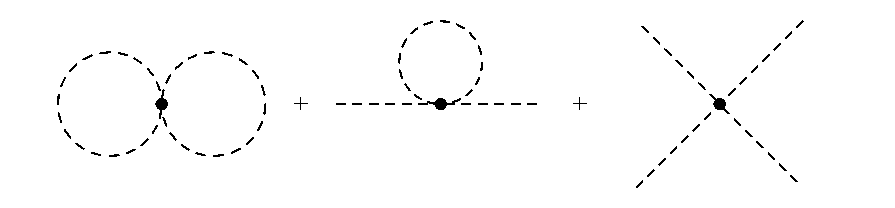
\includegraphics[scale=1]{图/phi4funcl.pdf}
	\caption{$\phi^4$相互作用一阶展开图}
\end{figure}
则生成泛函为：
% \begin{scriptsize}
	\begin{align}
	\mathscr{Z}[J]&=\frac{\displaystyle{1-\frac{ig}{4!}\int\mathrm{d}x\Big(3K(0)^2-6K(0)\Big[\int\mathrm{d}x'K(x-x')J(x')\Big]^2+\Big[\int\mathrm{d}x'K(x-x')J(x')\Big]^4\Big)+\cdots}}{\displaystyle {1-\frac{ig}{4!}\int\mathrm{d}x(3K(0)^2)+\mathcal{O}(g^2)+\cdots}}\notag\\
	&\times\exp\Big[-\frac{1}{2}\int J(x)K(x-x')J(x')\mathrm{d}x\mathrm{d}x'\Big]
	\end{align}
% \end{scriptsize}

若我们需要求解2点Green函数，则只需对上式生成泛函求2阶泛函导数：
\begin{align}
\mathscr{G}(x_1,x_2)&=\frac{\delta^2 \mathscr{Z}[J]}{i^2\delta J(x_1) J(x_2)}\Big|_{J=0}\notag\\
&=K(x_1-x_2)-\frac{ig}{4!}12K(0)\int\mathrm{d}x K(x_1-x)K(x-x_2)+\mathcal{O}(g^2)+\cdots
\label{eq:G2}
\end{align}
其首阶即为场的Feynman传播子，$g$的一次方项则表示为两个传播子中间加入一个内线圈图，更高阶图则对应于含有耦合常数更高次幂的项。对于生成泛函中的$g$的一次方项中的三项，真空项利用无真空项Green函数定义消去，而源的四次方项在2点Green函数求解中由于仍有多余的外源项化为0，但该项则会出现在4点Green函数中：
% \begin{footnotesize}
	\begin{align}
	\mathscr{G}(x_1,x_2,x_3,x_4)&=K(x_1-x_2)K(x_3-x_4)+K(x_1-x_3)K(x_2-x_4)+K(x_1-x_4)K(x_2-x_3)\notag\\
	&-\frac{ig}{4!}12\left(K(x_1-x_2)K(0)\int\mathrm{d}xK(x_3-x)K(x_4-x)+\text{5 permut.}\right)\notag\\
	&-\frac{ig}{4!}24\int\mathrm{d}x K(x_1-x)K(x_2-x)K(x_3-x)K(x_4-x)+\mathcal{O}(g^2)+\cdots
	\end{align}
% \end{footnotesize}
对于4点Green函数的首阶三项，其表示为两条互不相连的传播子。对于一阶项，其中6项由一条传播子和一条2点Green函数一阶项构成，且同样相互间不连接。这类图我们称为非连接图，是可以由一些其它连接的图组合而成。因此我们定义连接Green函数$G_{\text{c}}(x_1,\cdots,x_n)$，对于原Green函数，则有：
\begin{equation}
\mathscr{G}_n(x_1,\cdots,x_n)=\sum_{k=1}^{n}\sum_{n_k}(G_{\text{c}}(x_{i_1}\cdots, x_{i_{n_1}})\cdots G_{\text{c}}(x_{j_1}\cdots,x_{j_{n_k}})+\text{permut.})
\end{equation}
例如对于4点Green函数：
\begin{equation}
\mathscr{G}(x_1,x_2,x_3,x_4)=\Big(G_{\text{c}}(x_1,x_2)G_{\text{c}}(x_3,x_4)+\text{2 permut.}\Big)+G_{\text{c}}(x_1,x_2,x_3,x_4)+\cdots
\end{equation}
而4点连通Green函数则为：
% \begin{scriptsize}
\begin{align}
	&G_{\text{c}}(x_1,x_2,x_3,x_4)=\frac{-ig}{4!}\left(24\int\mathrm{d}x K(x_1-x)K(x_2-x)K(x_3-x)K(x_4-x)\right)\notag\\
	&+\frac{(-ig)^2}{(4!)^2}\left(288K(0)\int\mathrm{d}x\mathrm{d}x'K(x-x')K(x'-x_1)K(x-x_2)K(x-x_3)K(x-x_4)+\text{3 permut.}\right)\notag\\
	&+\frac{(-ig)^2}{(4!)^2}\Big(288\int\mathrm{d}x\mathrm{d}x'K(x-x_1)K(x-x_2)K(x-x')K(x'-x)K(x'-x_3)K(x'-x_4)\notag\\
	&\hspace{7.3cm}+\text{2 permut.}\Big)+\mathcal{O}(g^3)+\cdots
	\label{eq:G4}
	\end{align}
% \end{scriptsize}

同样我们可以有连通Green函数的生成泛函：
\begin{equation}
{W}[J]=\sum_{n}^{\infty}\frac{i^n}{n!}\int\mathrm{d}x_1\cdots\mathrm{d}x_n G_{\text{c}}(x_1\cdots x_n)J(x_1)\cdots J(x_n)
\end{equation}
因此我们可以利用上式连通Green函数求和定义式，将其与无真空项Green函数生成泛函$\mathscr{Z}[J]$相联系：
\begin{equation}
\mathscr{Z}[J]=e^{{W}[J]}
\end{equation}
则有：
\begin{equation}
{W}[J]=\ln\mathscr{Z}[J]=\ln \mathcal{Z}_0[J]+\ln\Big(1+\mathcal{O}(g)+\cdots\Big)+\text{const.}
\end{equation}
连通Green函数即表为：
\begin{align}
G_c(x_1,\cdots,x_n)&=\frac{\delta}{i\delta J(x_1)}\cdots\frac{\delta}{i\delta J(x_n)}\ln\mathscr{Z}[J]\Big|_{J=0}\notag\\
&=\frac{\delta^n W[J]}{i^n\delta J^n(x)}\Big|_{J=0}
\end{align}

\section{有效作用量}
\label{sc:effact}
对于连通Green函数的生成泛函$W[J]$，我们对源和场作勒让德变换：
\begin{align}
&\Gamma[\phi]+\int\mathrm{d}^4xJ(x)\phi(x)=\frac{1}{i}W[J]\notag\\
&\Gamma[\phi]=\frac{1}{i}W[J]-\int\mathrm{d}^4xJ(x)\phi(x)
\label{eq:effact}
\end{align}
得到关于场的泛函$\Gamma[\phi]$。则我们可得如下关系：
\begin{equation}
\frac{\delta W[J]}{i\delta J(x)}=\phi(x),\qquad\frac{\delta\Gamma[\phi]}{\delta\phi(x)}=-J(x)
\end{equation}
此时，由于理论的洛伦兹不变性，$\phi$场实际可以看成是静止场，由外源$J$与其产生相互作用。
\begin{itemize}
	\item 考虑Boson场：
\end{itemize}
由于对于自由场的$W[J]$，由\eqref{eq:zrbos}式我们可以有：
\begin{equation}
W[J]=-\frac{1}{2}\int J(x)\Delta(x-x')J(x')\mathrm{d}x\mathrm{d}x' + \text{const.}\label{eq:congreen}
\end{equation}
我们可得：
\begin{align}
\phi(x)&=\frac{\delta W[J]}{i\delta J(x)}=i\int \Delta(x-x')J(x')\mathrm{d}x'\\
J(x)&=\int\mathrm{d}x'\Delta^{-1}(x'-x)\phi(x')
\end{align}
由此可看出，该场可看成有外源时的经典场，满足方程$(\partial^\mu\partial_\mu+m^2)\phi(x)=J(x)$。此时，将上式入勒让德变换，泛涵$\Gamma[\phi]$则为：
\begin{equation}
\Gamma[\phi]=\int\left(-\frac{1}{2}\int\mathrm{d}x'\phi(x)\Delta^{-1}(x'-x)\phi(x')\right)\mathrm{d}x+\text{const.}
\end{equation}
\begin{itemize}
\item 对于Fermion场：
\end{itemize}
\begin{equation}
\Gamma[\phi]=\frac{1}{i}W[\eta,\bar{\eta}]-\int\mathrm{d}x \Big(\bar{\eta}(x)\psi(x)+\bar{\psi}(x)\eta(x)\Big)
\end{equation}
考虑在自由的情况下，由\eqref{eq:zfer}式，我们可得：
\begin{equation}
W[\bar{\eta},\eta]=-\int\bar{\eta}(x)S(x-x')\eta(x')\mathrm{d}x\mathrm{d}x'+\text{const.}
\end{equation}
那么我们则有：
\begin{align}
\psi(x)&=\frac{\delta W}{i\delta\bar{\eta}(x)}=i\int S(x-x')\eta(x')\mathrm{d}x',&\eta(x)&=-\int S^{-1}(x-x')\psi(x')\mathrm{d}x'\notag\\
\bar{\psi}(x)&=\frac{\delta W}{i\delta{\eta}(x)}=i\int \bar{\eta}(x')S(x-x')\mathrm{d}x',&\bar{\eta}(x)&=-\int \bar{\psi}(x')S^{-1}(x-x')\mathrm{d}x'
\end{align}
其中Dirac传播子的逆满足$\int\mathrm{d}z\,S^{-1}(x-z)S(z-y)=i\delta(x-y)$，与Boson场的形式并不相同。最终可解得泛函$\Gamma[\bar{\psi},{\psi}]$的形式为：
\begin{equation}
\Gamma[\bar{\psi},{\psi}]=\int\left(\int\mathrm{d}x'\bar{\psi}(x)S^{-1}(x-x')\psi(x')\right)\mathrm{d}x
\end{equation}
可以看出，在考虑自由场时泛涵$\Gamma[\phi]$具有自由作用量的形式，但是若引入相互作用之后，则会增加有效势项，因此也称为有效作用量。

我们可以对生成泛涵$W[J]$和有效作用量再作一阶泛函求导，可得2点连通Green函数以及函数$\bar{\Gamma}(x)$：
\begin{gather}
G_c(x_1,x_2)=\frac{\delta^2W}{i\delta J(x_1)i\delta J(x_2)}=\frac{\delta\phi(x_1)}{i\delta J(x_2)}\\
\bar{\Gamma}(x_1,x_2)=\frac{\delta^2\Gamma[\phi]}{\delta\phi(x_1)\delta\phi(x_2)}=-\frac{\delta J(x_1)}{\delta\phi(x_2)}
\end{gather}
由此可得函数$\bar{\Gamma}(x)$为连通Green函数的逆：
\begin{equation}
\int\mathrm{d}z G_c(x_1,z)\bar{\Gamma}(z,x_2)=i\delta(x_1-x_2)
\end{equation}

对于非自由的情况，则会产生更高阶的泛函导数项，现在考虑3点函数，则对下式两边同时求泛涵导数$\frac{\delta}{i\delta J(y)}$
\begin{equation}
\int\mathrm{d}z \;i\frac{\delta\phi(x_1)}{\delta J(z)}\frac{\delta J(z)}{\delta\phi(x_2)}=i\delta(x_1-x_2)
\end{equation}
可得：
\begin{equation}
\int\mathrm{d}z\left( \frac{\delta^2\phi(x_1)}{\delta J(y)\delta J(z)}\frac{\delta J(z)}{\delta\phi(x_2)}+\int\mathrm{d}x_3\frac{\delta\phi(x_1)}{\delta J(z)}\frac{\delta\phi(x_3)}{\delta J(y)}\frac{\delta^2J(z)}{\delta\phi(x_3)\delta\phi(x_2)} \right)=0
\end{equation}
将前式代入，则有：
% \begin{small}
	\begin{equation}
	\int\mathrm{d}z\left(\frac{\delta^3W[J]}{i^3\delta J(z)\delta J(y)\delta J(x_1)}\bar{\Gamma}(z,x_2)+\int\mathrm{d}x_3 \;G_c(x_1,z)G_c(x_3,y)\frac{\delta^3\Gamma[\phi]}{\delta\phi(x_3)\delta\phi(x_2)\delta\phi(z)}\right)=0
	\end{equation}
% \end{small}
再两边同乘$G_c(x_4,x_2)$，并对$x_2$积分，并替换变量名称，则最终得：
% \begin{footnotesize}
	\begin{equation}
	\frac{\delta^3W[J]}{i^3\delta J(z_3)\delta J(z_2)\delta J(z_1)}=\frac{1}{i}\int\mathrm{d}x_1\mathrm{d}x_2\mathrm{d}x_3 G_c(z_1,x_1)G_c(z_2,x_2)G_c(x_3,z_3)\frac{\delta^3\Gamma[\phi]}{\delta\phi(x_3)\delta\phi(x_2)\delta\phi(x_1)}
	\end{equation}
% \end{footnotesize}
即3点Green函数可表示为：
\begin{equation}
G_c(z_1,z_2,z_3)=\frac{1}{i}\int\mathrm{d}x_1\mathrm{d}x_2\mathrm{d}x_3 G_c(x_1,z_1)G_c(x_2,z_2)G_c(z_3,x_3)\bar{\Gamma}(x_1,x_2,x_3)
\end{equation}
\begin{figure}[H]
	\centering
 % \begin{fmffile}{3pvert}
 %       \begin{fmfgraph*}(100,100)
 %    \fmfbottom{x2,x1}
 %    \fmftop{x3}
 %    \fmf{plain,t=1}{x3,v3,v}
 %    \fmf{plain}{x2,v1}
 %    \fmf{plain,t=1}{v1,v,v2}
 %    \fmf{plain}{v2,x1}
 %    \fmfblob{100}{v1}
 %    \fmfblob{100}{v}
 %    \fmfblob{100}{v2}
 %    \fmfblob{100}{v3}
 %    \fmfv{d.sh=circle,d.f=1,d.si=5pt}{x1}
 %    \fmfv{d.sh=circle,d.f=1,d.si=5pt}{x2}
 %    \fmfv{d.sh=circle,d.f=1,d.si=5pt}{x3}
 %    \end{fmfgraph*}
 % \end{fmffile}
	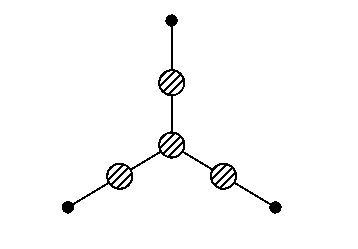
\includegraphics[scale=1]{图/3pvert.pdf}
	\caption{3点连通Green函数}
\end{figure}
而同样我们可利用互逆关系推导函数$\bar{\Gamma}(x_1,x_2,x_3)$：
\begin{equation}
\bar{\Gamma}(x_1,x_2,x_3)=-\int\mathrm{d}z_1\mathrm{d}z_2\mathrm{d}z_3 \bar{\Gamma}(z_1,x_1)\bar{\Gamma}(z_2,x_2)\bar{\Gamma}(z_3,x_3)G_c(z_1,z_2,z_3)
\end{equation}
对于3点Green函数，则可看成由3条外线传播子和内部结构组成，而函数$\bar{\Gamma}(x_1,x_2,x_3)$则表示了3点Green函数的内部结构。我们因此称之为3点单粒子不可约顶点函数。对于单粒子不可约图，指不能通过切开任意一条内线传播子而拆分成非连接图。

由此递推，我们可以推广到任意多外点，则有$n$点单粒子不可约顶点函数，简称$n$点顶点函数：
\begin{equation}
\bar{\Gamma}_n(x_1,\cdots x_n)=\frac{\delta^n\Gamma[\phi]}{\delta\phi_i(x_1)\cdots\delta\phi_j(x_n)}
\end{equation}
单粒子不可约可以按照阶次展开，首阶为数图不包含圈图，而每一阶对应了内部有多少个圈。而有效作用量$\Gamma[\phi]$则为其生成泛函：
\begin{equation}
\Gamma[\phi]=\sum_{n}\int\mathrm{d}x_1\cdots\mathrm{d}x_n\bar{\Gamma}_n(x_1\cdots x_n)\phi_i(x_1)\cdots\phi_j(x_n)
\end{equation}
若其中某一个顶点函数有$k$个全同性外线，则还需加上$\frac{1}{k!}$的因子。考虑只保留低阶展开项，而舍去高阶的多点函数项，则有效作用量可写成展开式的形式：
\begin{equation}
\Gamma[\phi]=\int\mathrm{d}x_1\mathrm{d}x_2\;\phi_i(x_1)\bar{\Gamma}_{ij}(x_1,x_2)\phi_j(x_2)+\int\mathrm{d}x_1\mathrm{d}x_2\mathrm{d}x_3\;\phi_i(x_1)\phi_j(x_2)\bar{\Gamma}_{ijk}(x_1,x_2,x_3)\phi_k(x_3)+\cdots
\end{equation}
\section{有效势能与Feynman规则}
当我们在有效作用量$\Gamma[\phi]$的框架下讨论时，由于我们考虑为静止场而忽略了场的运动学效应，相当于没有动能项，因此有效作用量也可以表示为有效势能的形式：
\begin{equation}
    \Gamma[\phi]=-\int\mathrm{d}^4x\,\mathscr{V}_\mathrm{eff}(\phi)\label{eq:veff0}
\end{equation}
我们可以定义动量空间中的单粒子不可约函数$\tilde{\Gamma}(p_1,\cdots,p_n)$，即为单粒子不可约函数$\bar{\Gamma}(x_1,\cdots x_n)$的动量空间变换:
\begin{equation}
(2\pi)^4\delta(p_1+\cdots+p_n)\tilde{\Gamma}(p)=\int\mathrm{d}x_1\cdots\mathrm{d}x_n\bar{\Gamma}(x_1,\cdots,x_n)e^{ip_1x_1+\cdots+p_nx_n}\label{eq:effvert}
\end{equation}
其中$(2\pi)^4\delta(p_1+\cdots+p_n)$是为了确保动量守恒。
当我们考虑静止场外线动量都为0时，带入上式则可以得到有效势能
\begin{equation}
    \mathscr{V}_\mathrm{eff}(\phi) = -\sum_n^\infty \frac{\phi^n}{n!} \bar{\Gamma}_{(n)}(p_{1,\cdots i}=0) \label{eq:effpot}
\end{equation}
此时，$\bar{\Gamma}_{(n)}(p_{1,\cdots i}=0) $包含了所有阶次项的n点函数，对于给定的n点函数，更多的内部动量$p_i$意味着更高阶的修正项。对于一个$\phi^4$理论，它的原始势能最高次项就是4次项，但是有效势能则可以包含更高次$\phi^n$。

当我们最终可以计算散射矩阵的时候，我们则需要以此计算可观测物理量。由于散射矩阵被定义在散射态上，而我们的散射态是用Fock空间的基表示，在Fock空间中，基矢即为能量本征态，也为动量本征态。因此如果我们的Green函数是定义在位形空间中的，这样计算起来将会非常不便。所以我们就考虑在动量空间中的Green函数。从前面的讨论我们已经知道，$n$点Green函数由更基础的2点Green函数及顶点函数所构成，因此我们只需要讨论基础的传播子和顶点函数的形式，便可用其推导任意点Green函数。



\subsection{粒子传播子}
我们考虑以$\phi^4$理论的实标量场为例。且考虑动量空间中的连通Green函数，则对连通Green函数作Fourier变换。对于2点Green函数：
\begin{multline}
G_{\text{c}}(p_1,p_2)=\int\mathrm{d}x_1\mathrm{d}x_2 e^{ip_1x_1+ip_2x_2}K(x_1-x_2)\\
-\frac{ig}{2}K(0)\int\mathrm{d}x_1\mathrm{d}x_2 e^{ip_1x_1+ip_2x_2}\int\mathrm{d}x K(x_1-x)K(x-x_2)+\mathcal{O}(g^2)+\cdots
\end{multline}
由于$K(x_1-x_2)$里包含对动量的积分
\begin{equation}
G_{\text{c}}(p_1,p_2)=\int\mathrm{d}x_1\mathrm{d}x_2 e^{ip_1x_1+ip_2x_2}\int\frac{\mathrm{d}p}{(2\pi)^4}e^{ip(x_1-x_2)}K(p)+\mathcal{O}(g)+\cdots
\end{equation}
则我们改变积分次序，先将关于位形变量进行积分，便可得动量空间中的2点连通Green函数：
% \begin{small}
	\begin{align}
	G_{\text{c}}(p_1,p_2)&=(2\pi)^4\delta(p_1+p_2)\Big(K(p_1)+K(p_1)\frac{gK(0)}{i2}K(p_1)+\cdots\Big)\notag\\
	&=(2\pi)^4\delta(p_1+p_2)\Big(\frac{i}{p_1^2-m^2+i\epsilon}+\frac{i}{p_1^2-m^2+i\epsilon}\frac{gK(0)}{i2}\frac{i}{p_1^2-m^2+i\epsilon}+\cdots	\Big)
	\end{align}
% \end{small}
对于2点Green函数，可以改写为级数求和形式：
\begin{align}
G_{\text{c}}(p_1,p_2)&=(2\pi)^4\delta(p_1+p_2)\frac{i}{p_1^2-m^2+i\epsilon}\Big(\sum_{n}(\frac{gK(0)}{i2}\frac{i}{p^2-m^2+i\epsilon})^n\Big)\notag\\
&=(2\pi)^4\delta(p_1+p_2)\frac{i}{p_1^2-m^2+i\epsilon}\Big(\frac{1}{1-\frac{gK(0)}{2}\frac{1}{p^2-m^2+i\epsilon}}\Big)\notag\\
&=(2\pi)^4\delta(p_1+p_2)\frac{i}{p_1^2-m^2-\frac{gK(0)}{2}+i\epsilon}
\end{align}
由此可看出，$\frac{gK(0)}{2}$可以作为传播子中粒子质量的修正项，而$\frac{gK(0)}{2}$则称之为粒子自能$\Sigma(p^2)$：
\begin{equation}
\Sigma(p^2)=\frac{g}{2}K(0)=\frac{g}{2}\int\frac{\mathrm{d}q}{(2\pi)^4}\frac{i}{q^2-m^2+i\epsilon}
\end{equation}
因此动量空间中的2点连通Green函数最终表示为：
\begin{equation}
G_{\text{c}}(p_1,p_2)=(2\pi)^4\delta(p_1+p_2)\frac{i}{p_1^2-m^2-\Sigma(p^2)+i\epsilon}
\end{equation}
其中$\delta(p_1+p_2)$表示粒子传播遵守动量守恒。因此我们也可以得知，对于任意动量空间中的$n$点Green函数，都会有$\delta(p_1+\cdots+p_n)$来满足动量守恒。由此我们可简化Green函数，定义$\tilde{G}_c(p)$有：
\begin{equation}
G_c(p_1,\cdots,p_n)=(2\pi)^4\delta(p_1+\cdots+p_n)\tilde{G}_c(p)
\end{equation}
则有：
\begin{equation}
\tilde{G}_c(p)=\frac{i}{p^2-m^2-\Sigma(p^2)+i\epsilon}
\end{equation}
对于Feynman规则，由于高阶修正项可以由首阶项作为基本形式来组合而成，因此我们选取2点连通Green函数的首阶项$\tilde{G}^{(0)}_{\text{c}}(p)$作为传播子的Feynman规则。

\subsection{相互作用顶点}
对于$\phi^4$理论的4点顶点函数，由于理论没有3相互作用顶点，因此我们通过\ref{sc:effact}节的递推关系可得：
\begin{equation}
\bar{\Gamma}(x_1,x_2,x_3,x_4)=\int\mathrm{d}z_1\mathrm{d}z_2\mathrm{d}z_3\mathrm{d}z_4\bar{\Gamma}(z_1,x_1)\bar{\Gamma}(z_2,x_2)\bar{\Gamma}(z_3,x_3)\bar{\Gamma}(z_4,x_4)G_{\text{c}}(z_1,z_2,z_3,z_4)
\end{equation}
结合\ref{eq:G4}式的结果，我们可计算得：
\begin{align}
&\bar{\Gamma}(x_1,x_2,x_3,x_4)\notag\\
&=-ig\int\mathrm{d}x\Big(\delta(x_1-x)\delta(x_2-x)\delta(x_3-x)\delta(x_4-x)\Big) \notag\\
&-\frac{g^2}{2}\int\mathrm{d}x\mathrm{d}x'K(x-x')K(x'-x)\Big(\delta(x_1-x)\delta(x_2-x)\delta(x_3-x')\delta(x_4-x')\notag\\
&\hspace{6.3cm}+\text{2 permut.}\Big)+\mathcal{O}(g^3)+\cdots
\end{align}
同样，我们可以对其作傅里叶变换：
\begin{align}
&\bar{\Gamma}(p_1,p_2,p_3,p_4)=\int\mathrm{d}x_1\mathrm{d}x_2\mathrm{d}x_3\mathrm{d}x_4 \bar{\Gamma}(x_1,x_2,x_3,x_4)e^{ip_1x_1+p_2x_2+p_3x_3+p_4x_4}\notag\\
=&-ig\int\mathrm{d}x e^{i(p_1+p_2+p_3+p_4)x}\notag\\
&-\frac{g^2}{2}\int\mathrm{d}x\mathrm{d}x'K(x-x')K(x'-x)\Big(e^{i(p_1+p_2)x}e^{i(p_3+p_4)x'}+\text{2 permut.}\Big)+\cdots
\end{align}
对于首阶项，积分直接化为$\delta(p_1+p_2+p_3+p_4)$。而对于二阶项，同样利用内线传播子$K(x-x')$的傅里叶展开式可得：
\begin{align}
&K(x-x')K(x'-x)e^{i(p_1+p_2)x}e^{i(p_3+p_4)x'}\notag\\
=&\int\frac{\mathrm{d}q}{(2\pi)^4}\frac{\mathrm{d}q'}{(2\pi)^4}K(q)K(q')e^{i(p_1+p_2+q'-q)x}e^{i(p_3+p_4+q-q')}
\end{align}
再对$x,x'$积分得到$\delta(p_1+p_2+q'-q)$和$\delta(p_3+p_4+q-q')$，再对$q'$积分便可得：
\begin{multline}
\bar{\Gamma}(p_1,p_2,p_3,p_4)=-ig(2\pi)^4\delta(p_1+p_2+p_3+p_4)\\
-\frac{g^2}{2}\int\mathrm{d}q\Big(K(q)K(q-p_1-p_2)+\text{2 permut.}\Big)\delta(p_1+p_2+p_3+p_4)+\cdots
\end{multline}
其中的$\delta(p_1+p_2+p_3+p_4)$同样是出于对动量守恒的要求。
那么对于$\phi^4$有：
\begin{equation}
\tilde{\Gamma}(p)=-ig-\frac{g^2}{2}\int\frac{\mathrm{d}q}{(2\pi)^4}\Big(K(q)K(q-\sqrt{s})+K(q)K(q-\sqrt{t})+K(q)K(q-\sqrt{u})\Big)+\mathcal{O}(g^3)+\cdots
\end{equation}
其中$s,t,u$为Mandelstam变量，即为\ref{eq:mdstv}式。以上即为顶点项及其修正。对于一般情况，顶点项为：
\begin{equation}
\tilde{\Gamma}(p)=\Gamma_{(0)}(g;p)+\Gamma_{(1)}(g^2;p)+\Gamma_{(2)}(g^3;p)+\cdots
\end{equation}
对于顶点修正项$\Gamma_{(1)}(g^2;p)+\mathcal{O}(g^3)$，在QED中我们一般称为辐射修正项。

同样对于Feynman规则而言，我们也只取顶点函数的首阶项作为基本形式。则$\Gamma_{(0)}(g;p)$即为顶点Feynman规则。
\subsection{外线}
由于散射矩阵并非完整的Green函数，而是截腿的Green函数，因此对于完整Green函数的外腿，需要进行修改才能作为散射矩阵的一部分进行计算。截腿Green函数即为所有的外线传播子都将被挖去Feynman传播子的部分，而只保留其自旋相关的部分，这样的Green函数部分称为外线。

对于一般的场而言，我们之前已知通用的形式为：
\begin{equation}
\phi_i(x)=\int\frac{\mathrm{d}\boldsymbol{p}}{(2\pi)^{3/2}\sqrt{2E(\boldsymbol{p})}}\left(R_i(\boldsymbol{p})a(\boldsymbol{p})e^{-ipx} +R_i^*(\boldsymbol{p})a^\dagger(\boldsymbol{p})e^{ipx} \right)
\end{equation}
而考虑动量空间的散射矩阵：
\begin{align}
S_{\beta\alpha}=&\left(\prod_{m}^{j=1} R^*(\boldsymbol{q}_j)i\Delta^{-1}(q_j)\right)\left(\prod_{n}^{i=1}R(\boldsymbol{p}_i)i\Delta^{-1}(p_i)\right)G_n(p_1\cdots p_n;q_1\cdots q_m)
\end{align}
由散射矩阵的形式我们可以看出，外线传播子中Feynman传播子部分相互抵消，剩下的部分变为外线函数。
\begin{itemize}
	\item 对于入射动量$\boldsymbol{p}$，外线表示为：
	\begin{equation}
	R(\boldsymbol{p})_i 
	\end{equation}
	\item 对于出射动量$\boldsymbol{q}$，外线表示为：
	\begin{equation}
	R^*(\boldsymbol{q})_i 
	\end{equation}
\end{itemize}

对于标量场而言，$R(\boldsymbol{p})$为1，因此外线也为1。

通过组合外线、传播子、顶点，我们便可以完整的计算散射矩阵，这种组合的方法便是Feynman图。而外线、传播子、顶点在散射矩阵中的具体形式则构成了基本的Feynman规则。


\section{散射理论}
上述部分我们讨论了散射矩阵以及散射矩阵的求解方法，及将散射矩阵转化为Green函数并进行求解。我们可以看到，体系的总Green函数中包含有非连通项，若具体的散射矩阵时，这些非连通项则对应为散射过程中未发生相互作用的过程。然而对于这些过程我们并不感兴趣，这也是我们定义连通Green函数的原因，因此我们对于散射矩阵同样也要单独考虑发生相互作用的部分。

我们可以直接地将散射矩阵分为两部分：
\begin{equation}
S=\mathbbm{1}+i\mathcal{T}
\end{equation}
实部的单位矩阵即描述未发生相互作用的非连通过程。而虚部的矩阵$\mathcal{T}$则描述了真正发生相互作用的散射过程。

对于散射矩阵我们有：
\begin{equation}
\langle \psi_f|S|\psi_i\rangle=\langle \psi_f|\psi_i\rangle+i\langle\psi_f|\mathcal{T}|\psi_i\rangle
\end{equation}
在前面的讨论中，我们可以明显的看到，在散射矩阵，也就是Green函数中存在着$\delta(p_1+\cdots+p_n)$函数，来确保动量守恒。那么对于散射矩阵而言，由此可得这样的$\delta$函数在存在于虚部中。则可以描述为：
\begin{equation}
i\langle\psi_f|\mathcal{T}|\psi_i\rangle=i(2\pi)^4\delta(p_f-p_i)\mathcal{M}_{fi}
\label{eq:scattT}
\end{equation}
$\mathcal{M}_{fi}$称之为散射振幅。因此我们可以定义跃迁几率为：
\begin{equation}
W_{fi}=\frac{|\langle\psi_f|\mathcal{T}|\psi_i\rangle|^2}{\langle\psi_f|\psi_f\rangle\langle\psi_i|\psi_i\rangle}
\end{equation}
跃迁几率统计了所有发生非平庸过程的概率。其中分母为归一化系数，对于散射态，我们有\footnote{利用箱归一化}：
\begin{equation}
\langle\psi_\alpha|\psi_\alpha\rangle=\langle \boldsymbol{p}_1,\cdots,\boldsymbol{p}_n|\boldsymbol{p}_1,\cdots,\boldsymbol{p}_n\rangle=n!2E(\boldsymbol{p}_1)\cdots 2E(\boldsymbol{p}_n)V^n
\end{equation}
而对于跃迁几率的分子部分，有：
\begin{align}
[\delta(p_f-p_i)]^2&=\delta(p_f-p_i)\int\frac{\mathrm{d}^4x}{(2\pi)^4}e^{i(p_f-p_i)}\notag\\
&=\frac{\delta(p_f-p_i)}{(2\pi)^4}\int\mathrm{d}^4x=\delta(p_f-p_i)\frac{VT}{(2\pi)^4}
\end{align}
我们可以看出，分子部分有时间依赖性，为了研究单位时间的跃迁几率，我们便定义了跃迁速率：
\begin{equation}
w_{fi}=\frac{W_{fi}}{T}=(2\pi)^4\delta(p_f-p_i)|\mathcal{M}_{fi}|^2 V\left(\frac{1}{n!}\prod_{i}^{n}\frac{1}{2E(\boldsymbol{p}_i)V}\right)\left(\frac{1}{m!}\prod_{j}^{m}\frac{1}{2E(\boldsymbol{q}_j)V}\right)
\end{equation}
此时我们讨论的跃迁速率是基于确定的初态和确定的末态定义的，一般情况下，我们研究具体问题的时候，初态往往是确定的，然而末态却是不定的，往往是在相空间中形成分布的。为了使我们能对整个相空间中的所有跃迁速率进行统计，我们定义单位相体积元的跃迁速率：
\begin{equation}
\mathrm{d}w_{fi}=w_{fi}\prod_{j}^m g_j\frac{V\mathrm{d}^3\boldsymbol{p}_j}{(2\pi)^3}
\end{equation}
我们将$n!$，$m!$和$g_j$整合起来，组成一个统计因子：
\begin{equation}
\textbf{s}=\frac{1}{n!m!}\prod_j^m g_j
\end{equation}
则：
\begin{align}
\mathrm{d}w_{fi}&=\textbf{s}(2\pi)^4\delta(p_f-p_i)|\mathcal{M}_{fi}|^2V\left(\prod_{i}^{n}\frac{1}{2E(\boldsymbol{p}_i)V}\right)\left(\prod_{j}^{m}\frac{\mathrm{d}^3\boldsymbol{q}_j}{(2\pi)^3 2E(\boldsymbol{q}_j)}\right)\notag\\
&=\textbf{s}|\mathcal{M}_{fi}|^2V\left(\prod_{\text{initial}}\frac{1}{2E(\boldsymbol{p})V}\right)\left((2\pi)^4\delta(p_f-p_i)\prod_{\text{final}}\frac{\mathrm{d}^3\boldsymbol{q}}{(2\pi)^3 2E(\boldsymbol{q})}\right)
\end{align}
其中：
\begin{equation}
\mathrm{d}Q_{\text{LIPS}}=(2\pi)^4\delta(p_f-p_i)\prod_{\text{final}}\frac{\mathrm{d}^3\boldsymbol{p}}{(2\pi)^3 2E(\boldsymbol{p})}
\label{eq:dlips}
\end{equation}
称之为末态Lorentz不变相空间测度。
\subsection{衰变宽度}
当我们考虑单粒子衰变的时候，初态只有一个粒子。则我们的单位相空间的跃迁速率即为：
\begin{equation}
\mathrm{d}w_{fi}(p\rightarrow q_1+\cdots+q_n)=\frac{\textbf{s}|\mathcal{M}_{fi}|^2}{2E(\boldsymbol{p})}\mathrm{d}Q_{\text{LIPS}}
\end{equation}
对于衰变过程中单位时间的衰变概率，即跃迁速率，我们称之为衰变宽度$\Gamma$。通常对于数量为$N$的粒子衰变，我们可以定义粒子寿命$\tau$：
\begin{equation}
N=N_0 e^{-\Gamma t},\qquad \tau=\frac{1}{\Gamma}
\end{equation}
而此时对于衰变过程而言，我们一般考虑衰变粒子静止，因此$E(\boldsymbol{p})=m$。我们单位相空间的微分衰变宽度可以写为：
\begin{equation}
\mathrm{d}\Gamma=\frac{\textbf{s}|\mathcal{M}_{fi}|^2}{2m}\mathrm{d}Q_{\text{LIPS}}
\end{equation}
\subsection{散射截面}
通常在对撞机物理中，我们将两个初态粒子相撞，发生散射。因此我们的初态粒子就只考虑2个，即考虑跃迁速率$\mathrm{d}w_{fi}(p_1+p_2\rightarrow q_1+\cdots+q_n)$。

对于入射的初态粒子，在实验上我们可以给出其亮度$L$，即单位时间穿过单位面积的粒子个数。若我们给定特定截面$\sigma$，则我们可以求得在特定体积内单位时间出现的粒子数$N=\sigma L$。然而对于我们的散射过程来说，这样的粒子数则取决于跃迁速率，则我们可以以此定义单位相空间的微分散射截面：
\begin{equation}
\mathrm{d}\sigma=\frac{\mathrm{d}w_{fi}}{L}
\end{equation}

而对于亮度我们则可考虑在实验室坐标系中表示，即粒子1轰击靶粒子2，其相对速度为$v_{12}$，则亮度为：
\begin{equation}
L=v_{12}\rho_1\rho_2 V
\end{equation}
那么对于这两个粒子的四动量内积，由于粒子而静止，我们有：
\begin{align}
p_1 \cdot p_2&=p_1^0 p_2^0-\boldsymbol{p}_1\cdot\boldsymbol{p}_2=p_1^0 p_2^0\notag\\
&=\frac{m_1}{\sqrt{1-v_{12}^2}}m_2
\end{align}
由于四动量内积具有Lorentz不变性，因此我们可得速度：
\begin{equation}
v_{12}=\frac{\sqrt{(p_1p_2)^2-m_1^2m_2^2}}{p_1p_2}
\end{equation}
而对于粒子密度，其具有Lorentz协变性，即$\rho=\frac{\rho_0}{\sqrt{1-v^2}}=\rho_0\frac{E}{m}$，则
\begin{equation}
\rho_1\rho_2=\frac{{\rho_1}_0{\rho_2}_0}{\sqrt{1-v_{12}^2}}=\frac{p_1p_2}{m_1m_2}{\rho_1}_0{\rho_2}_0=\frac{p_1p_2}{E_1E_2}\rho_1\rho_2
\end{equation}
对于Lorentz协变形式的粒子密度，即为$\rho=1/V$，则我们可得亮度为：
\begin{equation}
L=V\sqrt{(p_1p_2)^2-m_1^2m_2^2}\frac{1}{E_1 V E_2 V}
\end{equation}
将二体初态的跃迁速率带入，便可得单位相空间的微分散射截面：
\begin{equation}
\mathrm{d}\sigma=\frac{\textbf{s} |\mathcal{M}_{fi}|^2}{4\sqrt{(p_1p_2)^2-m_1^2m_2^2}}\mathrm{d}Q_{\text{LIPS}}
\label{eq:2bxs}
\end{equation}
\subsection{质心系与末态相空间}
当考虑具体动力学过程的时候，我们需要选取一个特定的参考系进行计算。一般情况我们选取质心系作为我们的参考系，即总动量为0，则$\boldsymbol{p}_i=\boldsymbol{p}_f=0$。若我们要计算最后总的散射截面或者衰变宽度等等可观测量，那么我们就要考虑对相空间积分。而考虑相空间积分时，就需要考虑末态动量的积分。
\subsubsection*{二体相空间}
若我们考虑最简单的末态形式，即末态只有两个粒子，由\eqref{eq:dlips}式我们的Lorentz不变相空间测度为：
\begin{equation}
\mathrm{d}Q_{\text{LIPS}}=(2\pi)^4\delta(q_1+q_2-p_i)\frac{\mathrm{d}^3\boldsymbol{q}_1}{(2\pi)^3 2E(\boldsymbol{q_1})}\frac{\mathrm{d}^3\boldsymbol{q_2}}{(2\pi)^3 2E(\boldsymbol{q}_2)}
\end{equation}
对于其中的$\delta$函数，我们可以分解为：
\begin{align}
\delta^4(q_1+q_2-p_i)&=\delta(E_1+E_2-E_i)\delta^3(\boldsymbol{q}_1+\boldsymbol{q}_2)\notag\\
&=\delta(\sqrt{m_3^2+\boldsymbol{q}_1^2}+\sqrt{m_4^2+\boldsymbol{q}_2^2}-E_i)\delta^3(\boldsymbol{q}_1+\boldsymbol{q}_2)
\end{align}
我们可以利用质心系的性质和动量守恒，使得我们考虑的所有可能的末态动量大小都一样，仅仅只有方向上的差别，这样我们便可以将对相空间的积分转化为对角度的积分上去。而对于Lorentz不变相空间测度，我们便可以先对$\boldsymbol{q}_2$进行积分:
\begin{equation}
\int\mathrm{d}Q_{\text{LIPS}}=\frac{\delta(\sqrt{m_3^2+\boldsymbol{q}_1^2}+\sqrt{m_4^2+\boldsymbol{q}_1^2}-E_i)}{(2\pi)^2}\frac{\mathrm{d}^3\boldsymbol{q_1}}{4E(\boldsymbol{q}_1)E(-\boldsymbol{q}_1)}
\end{equation}
由$\delta$函数的性质$\delta(f(x))=\underset{\text{root}}{\sum}\frac{\delta(x-x_0)}{|f'(x_0)|}$，我们可得：
\begin{equation}
\delta(\sqrt{m_3^2+\boldsymbol{q}_1^2}+\sqrt{m_4^2+\boldsymbol{q}_1^2}-E_i)=\frac{\delta(\boldsymbol{q}_1-\boldsymbol{p}^*_f)}{|\boldsymbol{p}^*_f|\frac{E_1(\boldsymbol{p}^*_f)+E_2(\boldsymbol{p}^*_f)}{E_1(\boldsymbol{p}^*_f)E_2(\boldsymbol{p}^*_f)}}
\end{equation}
\vspace{-1pt}
此处的根$\boldsymbol{p}^*_f$我们定义为：
\begin{equation}
|\boldsymbol{p}^*_f|=\frac{1}{2E_i}\sqrt{(E_i^2-(m_3+m_4)^2)(E_i^2-(m_3-m_4)^2)}
\end{equation}
这时我们在将$\boldsymbol{q}_1$在球坐标中展开$\mathrm{d}^3\boldsymbol{q}_1=|\boldsymbol{q}_1|^2\mathrm{d}|\boldsymbol{q}_1|\mathrm{d}\Omega$，然后对$|\boldsymbol{q}_1|$积分，得：
\begin{equation}
\int\mathrm{d}Q_{\text{LIPS}}=\frac{1}{4(2\pi)^2}\frac{|\boldsymbol{p}^*_f|}{E_i}\mathrm{d}\Omega
\end{equation}
\begin{itemize}
	\item 那么对于二体衰变过程，其衰变宽度可以表示为：
\end{itemize}
\begin{equation}
\Gamma=\int\frac{|\mathcal{M}_{fi}|^2|\boldsymbol{p}^*_f|}{32\pi^2m^2}\mathrm{d}\Omega
\end{equation}
\begin{itemize}
	\item 对于二体散射过程，我们可以得到其微分散射截面：
	\begin{equation}
	\frac{\mathrm{d}\sigma}{\mathrm{d}\Omega}=\frac{ |\mathcal{M}_{fi}|^2}{64\pi^2\sqrt{(p_1p_2)^2-m_1^2m_2^2}}\frac{|\boldsymbol{p}^*_f|}{E_1+E_2}
	\label{eq:difxsec}
	\end{equation}
\end{itemize}
为了进一步简化计算，考虑入射动量$p_1,p_2$和出射动量$q_1,q_2$，利用四动量守恒我们可以定义Mandelstam变量：
\begin{align}
s&=(p_1+p_2)^2=(q_1+q_2)^2\notag\\
t&=(p_1-q_1)^2=(q_2-p_2)^2\notag\\
u&=(p_1-q_2)^2=(q_1-p_2)^2
\label{eq:mdstv}
\end{align}
除此之外我们还有恒等式：
\begin{equation}
s+t+u=\sum_{\text{all}}m_i^2
\label{eq:madsum}
\end{equation}
由于这三个变量都为Lorentz不变量，因此我们可以在任意参考系中用其进行计算。通常我们将入射的总能量记为$\sqrt{s}$。
因此二体散射的微分散射截面可以表示为：
\begin{equation}
\frac{\mathrm{d}\sigma}{\mathrm{d}\Omega}=\frac{|\mathcal{M}_{fi}|^2}{64\pi^2 s}\frac{|\boldsymbol{p}_f^*|}{|\boldsymbol{p}_\mathrm{cm}|}%\sqrt{\frac{s^2-2s(m_3^2+m_4^2)+(m_3^2-m_4^2)^2}{s^2-2s(m_1^2+m_2^2)+(m_1^2-m_2^2)^2}}
\label{eq:difxsec2}
\end{equation}
其中$|\boldsymbol{p}_\mathrm{cm}|=|\boldsymbol{p}_1|=|\boldsymbol{p}_2|$为初态质心系动量
\subsection{光学定理}
根据量子力学的概率守恒定律，散射矩阵为幺正变换，具有幺正性：
\begin{equation}
    S^\dagger S =\mathbbm{1}
\end{equation}
由于$S=\mathbbm{1} + i\mathcal{T}$，则矩阵$\mathcal{T}$满足：
\begin{equation}
\mathcal{T}^\dagger \mathcal{T}=i(\mathcal{T}^\dagger-\mathcal{T})
\end{equation}
考虑将以上等式作用到初态和末态，可得：
\begin{equation}
    \langle \psi_f| \mathcal{T}^\dagger \mathcal{T} |\psi_i\rangle=i\langle \psi_f| \mathcal{T}^\dagger-\mathcal{T} |\psi_i\rangle
\end{equation}
对于等式左边，可以在算符中间插入完备集$\sum_n|n\rangle\langle n|$，得：
\begin{gather}
    \sum_n \langle \psi_f| \mathcal{T}^\dagger|n\rangle \langle n| \mathcal{T} |\psi_i\rangle=i\langle \psi_f| \mathcal{T}^\dagger|\psi_i\rangle-i\langle \psi_f|\mathcal{T} |\psi_i\rangle\\
        \sum_n\left( \prod_{j=1}^n\int\frac{d^3 \boldsymbol{k}_j}{(2\pi)^3}\frac{1}{2E_j} \right) \langle \psi_f| \mathcal{T}^\dagger|\{\boldsymbol{k}_j\}\rangle \langle \{\boldsymbol{k}_j\}| \mathcal{T} |\psi_i\rangle=i\langle \psi_f| \mathcal{T}^\dagger|\psi_i\rangle-i\langle \psi_f|\mathcal{T} |\psi_i\rangle
\end{gather}
且由\eqref{eq:scattT}式，可得散射振幅之间的关系：
\begin{equation}
    \sum_n \int\mathrm{d}Q_n \mathcal{M}^*(\psi_f\rightarrow n) \mathcal{M}(\psi_i\rightarrow n) = i[\mathcal{M}^*(\psi_f\rightarrow\psi_i) - \mathcal{M}(\psi_i\rightarrow\psi_f)]
    \label{eq:optthe1}
\end{equation}
如果考虑弹性前向散射，即出射动量等于入射动量$p_f=p_i$，\eqref{eq:optthe1}式可化简为：
\begin{equation}
    \sum_n \int\mathrm{d}Q_n |\mathcal{M}(\psi_i\rightarrow n)|^2=2\operatorname{Im}\mathcal{M}(\psi_i\rightarrow\psi_i)
\end{equation}
进一步，我们可以考虑二体散射，即$|\psi_i\rangle = |p_1 p_2\rangle$，则可以引用\eqref{eq:2bxs}式中的二体散射截面，可得：
\begin{equation}
    2\sqrt{s} |\boldsymbol{p}_\mathrm{cm}| ~\sigma(p_1,p_2\rightarrow n) = \operatorname{Im}\mathcal{M}(p_1 p_2 \rightarrow p_1 p_2)
    \label{eq:optth}
\end{equation}
因此产生所以可能末态的二体散射的总散射截面可以通过前向散射的散射振幅虚部求得，此定理即为光学定理。

对于散射振幅而言，我们可以将其进行分波展开：
\begin{equation}
    \mathcal{M}_{if} = \sum_{\ell=0}^{\infty}(2\ell + 1 )a_\ell P_\ell(\cos\theta)
\end{equation}
则带入到二体散射截面\eqref{eq:difxsec2}式中，我们可以得到\footnote{对Legendre多项式，有：\[
\int P_n (x) P_m(x) \mathrm{d}x = \frac{2}{2n + 1}\delta_{n m}
\]}：
\begin{equation}
    \sigma_{if} = \frac{1}{32\pi s} \frac{|\boldsymbol{p}_f^*|}{|\boldsymbol{p}_\mathrm{cm}|}\int|\mathcal{M}_{if}(\cos\theta)|^2 \mathrm{d}\cos\theta = \frac{1}{16\pi s}\frac{|\boldsymbol{p}_f^*|}{|\boldsymbol{p}_\mathrm{cm}|} \sum_{\ell=0}^{\infty}(2\ell + 1 )|a_\ell|^2
\end{equation}
考虑二体弹性前向散射，则有$|\boldsymbol{p}_f^*| = |\boldsymbol{p}_\mathrm{cm}| = \frac{\sqrt{s}}{2}$， 且$\theta=0$，则由光学定理\eqref{eq:optth}式得：
\begin{align}
    \sigma_{ii} &= \frac{1}{s}\operatorname{Im}{\mathcal{M}_{ii}}\notag\\
    \frac{1}{16\pi s}\sum_\ell (2\ell + 1) |a_\ell|^2 &= \frac{1}{s}\sum_\ell (2\ell +1 )\operatorname{Im}(a_\ell)\notag\\
    \operatorname{Re}(a_\ell) ^2 + \operatorname{Im}(a_\ell) ^2 &= 16\pi \operatorname{Im}(a_\ell)
\end{align}
此时我们得到一个关于$\operatorname{Im}(a_\ell)$的二次函数，其中可以得到$\operatorname{Re}(a_\ell)$的极大值：
\begin{equation}
    \operatorname{Re}(a_\ell) \leq 8\pi
\end{equation}
因此对于二体弹性前向散射的振幅，其中的0阶振幅存在上限值，这样的约束条件即为幺正性条件：
\begin{equation}
    |\mathcal{M}_{ii}(\theta = 0, \ell = 0)| \leq 8\pi
\end{equation}


\chapter{重整化理论}
在之前动力学过程的讨论中，我们已经知道Green函数中的高阶项中会出现对内线动量积分项，即可以用Feynman图中的圈图来表示。我们之前并没直接求解这些积分项，并认为这些项由于耦合常数的高级次因子而使其大大压低，为高阶小量。然而我们实际去计算这些所谓的高阶小量时，却发现这些项由于是对所有可能的内线动量积分，且进行全域积分，因此这些项或多或少的会出现积分不收敛的情况，这显然与微扰展开的初衷相互矛盾。由此为了使理论自洽，我们则要具体讨论如何处理这些发散的积分项，并且得到这些项中真正对物理观测有实际效应的结果。
\section{量纲分析及表观发散度}
通常情况下内线动量积分项的发散往往来自于被积函数的形式，不同形式的被积函数也会呈现不同形式不同位置的发散。当我们分析内线动量积分项的发散形式以及发散程度，由于积分元为动量，因此我们分析被积函数的动量量纲，便可粗糙的推测积分项总体关于动量的量纲，由此即可得出积分项的发散形式。

如果我们考虑一个任意的Feynman图中，有$I$条内线传播子，同时有$V$个顶点。那么我们由动量守恒可知，$V$个顶点及$I$条内线传播子中只有$I-V+1$个独立动量，以此独立内线动量个数$L$可以表示为：
\begin{equation}
L=I-V+1
\end{equation}
这时我们考虑积分项，那么我们便需要对所有的独立内线动量进行积分，假设我们考虑在$d$维时空中，那么积分测度的量纲便为$[dL]$\footnote{此处的量纲为指数量纲，即动量的几次方的量纲即为其指数幂，而量纲之间的相乘则变为指数幂的相加。}。考虑被积函数的量纲，被积函数通常为内线传播子及顶点函数的乘积。而对于任意一个传播子，Boson传播子的量纲则为[-2]，Fermion传播子的量纲则为[-1]。而顶点函数，我们设其依赖于动量的$n$次方。那么被积函数的总量纲便可表示为$[nV-2I_{\text{B}}-I_{\text{F}}]$。最后综合上述结果，我们可以得到内线动量积分项的量纲为：
\begin{equation}
D=dL-2I_{\text{B}}-I_{\text{F}}+nV
\end{equation}
$D$即称为\emph{表观发散度}。我们可以用$D$来粗略地描述内线动量积分项的发散形式：
\begin{itemize}
	\item $D>0$时，积分项具有$\displaystyle{\int^\Lambda_0\frac{(\mathrm{d}^d p)^L}{p^{2I_{\text{B}}+I_{\text{F}}-V}}\sim \Lambda^D}$的形式。
	\item \(D=0\)时，积分项具有\(\displaystyle{\int^\Lambda_0\frac{(\mathrm{d}^d p)^L}{p^{2I_{\text{B}}+I_{\text{F}}-V}}\propto\int^\Lambda_0\frac{\mathrm{d}p}{p}\sim \ln\Lambda}\)的形式。
	\item \(D<0\)时，积分项具有$\displaystyle{\int^\Lambda_0\frac{(\mathrm{d}^d p)^L}{p^{2I_{\text{B}}+I_{\text{F}}-V}}\sim \frac{1}{\Lambda^D}}$的形式。
\end{itemize}

然而很多时候，这样的估算并不完全正确。有时候当整个Feynman图中有内部发散子图的结构，则对整体Feynman图的表观发散度就并非实际的发散度。又例如当我们计算得Feynman图表观发散度时，实际的Feynman图又可能因为对称性而将发散项消去了。

但是表观发散度这个物理量并非没有用处，我们可以进一步推导上述关系式。
\begin{equation}
D=(d-2)I_\text{B}+(d-1)I_\text{F}-dV+nV+d
\end{equation}
考虑有$E$条外线传播子，而对于每个相互作用顶点而言，其连接的Boson个数为\(N_\text{B}\)，连接的Fermion个数为\(N_{\text{F}}\)（必为偶数）。那么我们可以有关系：
\begin{equation}
N_\text{B}V=2I_\text{B}+E_\text{B},\qquad N_\text{F}V=2I_\text{F}+E_\text{F}
\end{equation}
反解出$I_\text{B}$和$I_{\text{F}}$，带入到表观发散度中：
\begin{equation}
D=d-\frac{d-2}{2}E_\text{B}-\frac{d-1}{2}E_\text{F}-\left(d-\frac{d-2}{2}N_\text{B}-\frac{d-1}{2}N_\text{F}-n\right)V
\end{equation}
对于顶点个数前的因子，我们可以探讨其具体意义。当我们考虑量子场理论在$d$维时空中的量纲分析，由于作用量为无量纲量，则Lagrangian的量纲为$[\mathscr{L}]=d$。那么Boson场函数的量纲为$[\phi]=\frac{d-2}{2}$，而Fermion场函数的量纲则为$[\psi]=\frac{d-1}{2}$。那么当我们考虑相互作用项时，势函数$V(\phi,\psi)$包含$N_\text{B}$个Boson场函数和$N_\text{F}$个Fermion场函数，以及还可能包含动量的$n$次方。由于势函数的量纲$[V]=d$，那么最后剩下的耦合常数的量纲则恰好为：
\begin{equation}
[g]=d-\frac{d-2}{2}N_\text{B}-\frac{d-1}{2}N_\text{F}-n
\end{equation}
则表观发散度可以表为：
\begin{equation}
D=d-\frac{d-2}{2}E_\text{B}-\frac{d-1}{2}E_\text{F}-[g]V
\end{equation}
可以看出，表观发散度除了依赖于时空维度$d$和外线个数$E$，这些外部给定的条件以外，还依赖于耦合常数的量纲，这样的理论本身的参数。因此我们可知，当耦合常数量纲为非0值时，表观发散度便会依赖于Feynman图中的顶点个数，即不同顶点个数的图会有不同的发散程度。我们可以总结得：
\begin{itemize}
	\item \([g]<0\)，表观发散度随着顶点个数增加而增加，意味着越高级次的Feynman图具有更高的发散程度，并且有无限多个发散Feynman图。那么理论上难以完整的处理所有发散图。
	\item \([g]>0\)，表观发散度随顶点个数增加而减少，意味着级次高到一定程度时Feynman图就不会发散。那么就只会有有限个数的发散Feynman图。
	\item \([g]=0\)，表观发散度完全不依赖于顶点个数，那么同一Green函数下的所有级次都具有同一种发散度，那么我们可以进行普适化处理，用同一种方法处理所有的发散项。满足这样条件的理论便称为\emph{可重整化理论}。
\end{itemize}

对于$[g]=0$的理论，若表观发散度$D\geqslant0$，存在发散。为了处理这些发散项，让我们得到有限的可观测量，我们便引入一些额外的抵消项，将发散消去。同时因为发散程度不依赖于级次，我们可以对所有级次引入相同形式的抵消项。这样的处理过程称之为\emph{重整化}。
\section{正规化及重整化方案}
对于圈积分，通常由于其发散的存在，我们难以直接对其求定积分结果。然而，我们可以通过一定的数学上的处理，使得我们可以求得积分的形式上的结果。即称为\emph{正规化}过程。

而在得到圈积分的形式解之后，我们便需要考虑如何将发散项分离，并且抵消。我们之所以要对我们的计算结果进行重整化，是因为虽然我们的圈积分形式解为无穷大，但是其仍然保留了我们需要的物理信息，能够对我们测量的可观测量有实在的贡献。然而因为我们的理论计算过程中会不可避免的引入真空项的贡献，才导致了这些发散项的存在。因此我们对理论进行再次的归一化操作，即保留圈积分中实在物理贡献，然后将圈积分“等比例缩放”。这便是重整化的意义所在。

由于重整化实质上是人为的引入抵消项消去发散，因此对于可重整化的理论而言，重整化的方法往往是不唯一的。换言之就是人为引入的抵消项存在多种可能的形式，而这是因为我们可以有不同的方法将理论中的发散项抵消掉，即会导致用于消去发散项的抵消项形式不同。因此我们会有多种可行的\emph{重整化方案}。
\subsection*{截断方案与正规化因子}
最简单直接的正规化方法，便是直接将对动量的无穷积分的上限作截断：
\begin{equation}
I(p)=\int_0^\infty\frac{\mathrm{d}k}{(k+p)^\alpha}\rightarrow\int_0^\Lambda\frac{\mathrm{d}k}{(k+p)^\alpha}
\end{equation}
这样我们便将形式上的无穷积分改为形式上的定积分，便可得到该积分的形式上的结果$I(p,\Lambda)$。这样的积分结果将用截断动量$\Lambda$来参数化，而我们最终的物理结果便是取$\Lambda$的无穷极限便可:
\begin{equation}
I(p)=\lim_{\Lambda\rightarrow\infty}I(p,\Lambda)
\end{equation}

在上述得到积分形式解的过程中，我们把将某些量进行参数化，而这样的参数便称为\emph{正规化因子}。例如截断中的截断能标$\Lambda$。对于任意一种正规化方法，都会有对应的正规化因子。但是物理的可观测量应该不依赖于人为设定的正规化因子，因此在重整化完成后，仍保留着的正规化因子可以通过取极限的方法取作特定值，便可得最终的具有物理意义的结果。

然而，截断并不是一种理想的正规化方法。因为当我们将极高速动量对积分的贡献人为忽略的时候，意味着高速动量和低速动量直接的Lorentz对称性遭到了破坏，这样显然与理论本身矛盾。

不仅如此，有些正规化方法虽然可以保留Lorentz对称性，但是却会破坏场的规范对称性。因此选择正规化重整化方案的时候我们需要谨慎考虑其对于理论的各种对称性的影响。

\section{单圈修正及重整化}
\subsection*{维数正规化}
对于单圈图的计算，最常用的正规化方法则是维数正规化。维数正规化方法最大的优势便是可以不破坏Lorentz对称性和规范对称性，因此这样的方法成为了最常用的方法。

维数正规化，即是考虑对于圈积分中的4维积分测度，我们将其推广到一般情况的$d$维，在计算完成之后，再将其回归到4维情况。考虑一般形式的单圈积分：
\begin{gather}
I^{\mu_1\cdots\mu_m}(p_1\cdots p_n,d)=\int\frac{\mathrm{d}^d k}{(2\pi)^d}\frac{k^{\mu_1}\cdots k^{\mu_m}}{((k+p_1)^2-m_1^2)^{\alpha_1}\cdots((k+p_n)^2-m_n^2)^{\alpha_n}}\notag\\
\label{eq:loopint}
\end{gather}
其中考虑$n$个外线动量$p$以及一个内线动量的积分，而圈中的包含任意一外线动量$p_i$的传播子出现了$\alpha_i$次。而分子上的动量项则表示为传播子的Lorentz结构。

先考虑包含单一外线动量的单圈积分，且暂时不考虑该传播子的Lorentz结构，那么我们有单圈积分最基础的形式：
\begin{align}
I(p,d)&=\int\frac{\mathrm{d}^d k}{((k+p)^2-m^2)^\alpha}\notag\\
&=\int\frac{\mathrm{d}^d k}{(k^2+2k\cdot p-\omega^2)^\alpha}
\end{align}
其中我们将与积分无关的项视为常数$\omega^2=m^2-p^2$。

那么我们可以考虑对内线动量作平移$k\rightarrow k-p$，积分测度保持不变。由于该积分是定义在Minkowski空间中，并不方便进行处理，所以我们对$k^0$分量作Wick转动$k^0\rightarrow ik^0$，使积分变为欧几里得空间的积分：
\begin{equation}
I(d)=\int\frac{\mathrm{d}^d k}{(k^2-m^2)^\alpha}=i(-1)^\alpha\int\frac{\mathrm{d}^d k}{(k^2+m^2)^\alpha}
\label{eq:int1}
\end{equation}
我们考虑$d$维球坐标，测度可以表为：
\begin{equation}
\mathrm{d}^dk=k^{d-1}\mathrm{d}k\,\mathrm{d}\phi\prod_{i=1}^{d-2}\sin^i\theta\mathrm{d}\theta
\end{equation}
带入积分中，可以直接将$\phi$角积分得到$2\pi$。而对$\theta$角的积分则得
\begin{equation}
\prod_{i=1}^{d-2}\int_0^\pi\sin^i\theta\mathrm{d}\theta=\frac{\pi^\frac{d-2}{2}}{\Gamma(\frac{d}{2})}
\end{equation}
这样我们可得：
\begin{equation}
I(d)=(-1)^\alpha i\frac{2\pi^{\frac{d}{2}}}{\Gamma(\frac{d}{2})}\int_0^\infty\frac{k^{d-1}\mathrm{d}k}{(k^2+m^2)^\alpha}
\end{equation}
我们将内线动量换元$t=k/m$，则可得：
\begin{equation}
I(d)=(-1)^\alpha i\frac{2\pi^{\frac{d}{2}}m^{d-2\alpha}}{\Gamma(\frac{d}{2})}\int_0^\infty\mathrm{d}t\; t^{d-1}(1+t^2)^{-\alpha}
\end{equation}
引用Euler积分\footnote{\begin{itemize}
		\item 第一类Euler积分（Euler-Beta函数）：\[\mathrm{B}(x,y)=\int_0^\infty\mathrm{d}t\;t^{x-1}(1+t)^{-x-y}\]
		\item 第二类Euler积分（Gamma函数）：\[\Gamma(x)=\int_0^\infty\mathrm{d}t\;t^{x-1}e^{-t}\]
	\end{itemize}
	且有\vspace{-8pt}\[\mathrm{B}(x,y)=\frac{\Gamma(x)\Gamma(y)}{\Gamma(x+y)}\]}
可得最终积分结果：
\begin{align}
I(d)=&(-1)^\alpha i\frac{\pi^{\frac{d}{2}}m^{d-2\alpha}}{\Gamma(\frac{d}{2})}\mathrm{B}\left(\frac{d}{2},\alpha-\frac{d}{2}\right)\notag\\
&=(-1)^\alpha i\pi^{\frac{d}{2}}m^{d-2\alpha}\frac{\Gamma(\alpha-\frac{d}{2})}{\Gamma(\alpha)}
\label{eq:int1re}
\end{align}

然而对于一般形式的单圈积分，即包含多种不同外线动量的传播子相乘的形式，情况则会有所不同。同样我们先不考虑分子的Lorentz结构，有：
\begin{equation}
I_n(d)=\int\frac{\mathrm{d}^dk}{(2\pi)^d}\frac{1}{(\Delta_1^{-1})^{\alpha_1}\cdots(\Delta_n^{-1})^{\alpha_n}},\qquad (\Delta^{-1}_n)^{\alpha_n}=(k^2+2k\cdot p_n-\omega_n^2)^{\alpha_n}
\end{equation}
对于两项不同传播子项之积，我们可以引入辅助量将其转化为和的形式\footnote{\[\frac{1}{ab}=\int_0^1\frac{\mathrm{d}x}{[ax+b(1-x)]^2}\]}。而对于$n$项传播子之积，则有：
% \begin{small}
	\begin{equation}
	\frac{1}{(\Delta_1^{-1})^{\alpha_1}\cdots(\Delta_n^{-1})^{\alpha_n}}=\frac{1}{\prod_i\Gamma(\alpha_i)}\int_0^1\mathrm{d}x_2\cdots\mathrm{d}x_n\prod_{i=1}^n x_i^{\alpha_i-1}\int_0^\infty\mathrm{d}t\;t^{\sum\alpha_i-1}e^{-(\Delta^{-1}_ix_i)t}
	\end{equation}
% \end{small}
其中辅助量$x_i$有条件$\sum_i x_i=1$。再将辅助量$t$进行变换$t\rightarrow t/(\Delta^{-1}_ix_i)$，可得：
% \begin{small}
	\begin{align}
	\frac{1}{(\Delta_1^{-1})^{\alpha_1}\cdots(\Delta_n^{-1})^{\alpha_n}}=\frac{1}{\prod_i\Gamma(\alpha_i)}\int_0^1\frac{\mathrm{d}x_2\cdots\mathrm{d}x_n}{(\sum_j \Delta_j^{-1}x_j)^{\sum\alpha_i}}\prod_{i=1}^n x_i^{\alpha_i-1}\int_0^\infty\mathrm{d}t\;t^{\sum\alpha_i-1}e^{-t}\notag\\
	\end{align}
% \end{small}
将$\sum_i x_i=1$约束条件放入式子中，并整理可得：
\begin{equation}
I_n(d)=\int\frac{\mathrm{d}^dk}{(2\pi)^d}\Big(\frac{\Gamma(\sum_i\alpha_i)}{\prod_i\Gamma(\alpha_i)}\int_0^1\frac{\prod_{i=1}^n(\mathrm{d}x_i x_i^{\alpha_i-1})\delta(\sum_i x_i-1)}{[k^2+2k\cdot(\sum x_ip_i)-\sum_i x_i\omega_i^2]^{\alpha_1+\cdots+\alpha_n}}\Big)
\end{equation}
即称为Feynman圈积分公式。

若考虑传播子不同的Lorentz结构，鉴于\eqref{eq:loopint}式，我们可以定义一个辅助的圈积分生成函数：
\begin{equation}
I^m_n(\ell,d)=\int\frac{\mathrm{d}^d k}{(2\pi)^d}(k\cdot\ell)^m\prod_{i=1}^n\frac{1}{(k^2+2k\cdot p_i-\omega_i^2)^{\alpha_i}}
\end{equation}
这样一般形式的圈积分分子中的Lorentz结构便可以由其求导生成：
\begin{equation}
I^{\mu_1\cdots\mu_m}_n=\frac{1}{m!}\frac{\partial^m I^m_n(\ell)}{\partial\ell_{\mu_1}\cdots\partial\ell_{\mu_m}}
\end{equation}

我们可以直接求解圈积分生成函数，实际上即为无分子动量项圈积分乘上$(k\cdot\ell)^m$。由上述Feynman圈积分公式结果，我们改变积分次序，可以化为：
% \begin{footnotesize}
	\begin{equation}
	I^m_n(\ell,d)=\frac{\Gamma(\sum_i\alpha_i)}{\prod_i\Gamma(\alpha_i)}\int_0^1\prod_{i=1}^n(\mathrm{d}x_i x_i^{\alpha_i-1})\delta(\sum_i x_i-1)\Big(\int\frac{\mathrm{d}^dk}{(2\pi)^d}\frac{(k\cdot\ell)^m}{[(k+\sum x_ip_i)^2-\Omega]^{\sum_i\alpha_i}}\Big),
	\end{equation}
% \end{footnotesize}
\begin{equation}
\Omega\equiv\sum x_i\omega_i^2+(\sum x_i p_i)^2
\end{equation}
仿照之前的单外线动量圈积分，我们对内线动量作平移变换$k\rightarrow k-\sum x_ip_i$，可得：
% \begin{small}
	\begin{align}
	I^m_n(\ell,d)=&\frac{\Gamma(\sum_i\alpha_i)}{\prod_i\Gamma(\alpha_i)}\int_0^1\prod_{i=1}^n(\mathrm{d}x_i x_i^{\alpha_i-1})\delta(\sum_i x_i-1)\Big(\int\frac{\mathrm{d}^dk}{(2\pi)^d}\frac{(k\cdot\ell-(\sum x_ip_i)\cdot\ell)^m}{[k^2-\Omega]^{\sum_i\alpha_i}}\Big)\notag\\
	=&\frac{\Gamma(\sum_i\alpha_i)}{\prod_i\Gamma(\alpha_i)}\int_0^1\prod_{i=1}^n(\mathrm{d}x_i x_i^{\alpha_i-1})\delta(\sum_i x_i-1)\notag\\
	&\times\sum_{r=0}^{m}(-1)^{m-r}C_m^r(\sum x_ip_i\cdot\ell)^{m-r}\Big(\int\frac{\mathrm{d}^dk}{(2\pi)^d}\frac{(k\cdot\ell)^r}{[k^2-\Omega]^{\sum_i\alpha_i}}\Big)
	\end{align}
% \end{small}
由于当$r$为奇数时，被积函数为奇函数，这时我们对全空间的积分就会变为0。所以只有$r$为偶数时才有非0结果。所以我们改写为：
\begin{multline}
I^m_n(\ell,d)=\frac{\Gamma(\sum_i\alpha_i)}{\prod_i\Gamma(\alpha_i)}\int_0^1\prod_{i=1}^n(\mathrm{d}x_i x_i^{\alpha_i-1})\delta(\sum_i x_i-1)\\\times\sum_{r=0}^{[\frac{m}{2}]}(-1)^{m-2r}C_m^{2r}(\sum x_ip_i\cdot\ell)^{m-2r}\Big(\int\frac{\mathrm{d}^dk}{(2\pi)^d}\frac{(k\cdot\ell)^{2r}}{[k^2-\Omega]^{\sum_i\alpha_i}}\Big)
\end{multline}
对于积分部分，形式上与\eqref{eq:int1}式类似，但是分子形式不同。此时我们可将分子部分化为：
\begin{equation}
(k\cdot\ell)^{2r}=\frac{(\ell^2)^r(k^2)^r}{d(d+2)\cdots(d+2(r-1))}\frac{(2r)!}{2^r r!}
\end{equation}
便可将式子化为：
\begin{align}
I^m_n(\ell,d)&=\frac{\Gamma(\sum_i\alpha_i)}{\prod_i\Gamma(\alpha_i)}\int_0^1\prod_{i=1}^n(\mathrm{d}x_i x_i^{\alpha_i-1})\delta(\sum_i x_i-1)\notag\\
&\times\sum_{r=0}^{[\frac{m}{2}]}\frac{(-1)^{m-2r}C_m^{2r}(\sum x_ip_i\cdot\ell)^{m-2r}(\ell^2)^r(2r)!}{d(d+2)\cdots(d+2(r-1))2^r r!}\Big(\int\frac{\mathrm{d}^dk}{(2\pi)^d}\frac{(k^2)^{r}}{[k^2-\Omega]^{\sum_i\alpha_i}}\Big)
\end{align}
这样我们就能得到相似于\eqref{eq:int1}式的积分形式。和得到\eqref{eq:int1re}式结果的过程一样，我们用相同的方法得到该积分的结果：
\begin{equation}
\int\frac{\mathrm{d}^dk(k^2)^{r}}{[k^2-\Omega]^{\sum_i\alpha_i}}=i(-1)^{r+\sum_i\alpha_i}\pi^{\frac{d}{2}}\frac{\Gamma(\sum_i\alpha_i-r-\frac{d}{2})\Gamma(r+\frac{d}{2})}{\Gamma(\frac{d}{2})\Gamma(\sum_i\alpha_i)}\Omega^{r+\frac{d}{2}-\sum_i\alpha_i}
\end{equation}
代入回原式，最终我们整理可得：
%\begin{small}
\begin{multline}
	I^m_n(\ell,d)=\frac{i(-1)^{m+\sum_i\alpha_i}}{(4\pi)^{\frac{d}{2}}\prod_i\Gamma(\alpha_i)}\int_0^1\prod_{i=1}^{n}(\mathrm{d}x_i\;x_i^{\alpha_i-1})\delta(\sum_i x_i-1)\Omega^{\frac{d}{2}-\sum_i\alpha_i}\\\times\sum_{r=0}^{[\frac{m}{2}]}(-1)^r\frac{(2r)!}{4^r r!}C^{2r}_m(\sum x_ip_i\cdot\ell)^{m-2r}\Gamma(\sum_i\alpha_i-r-\frac{d}{2})(\ell^2)^r\Omega^{r}
	\label{eq:feyint}
\end{multline}
%\end{small}
此时圈积分依然是维数$d$的函数，那么现在我们让维数回归到我们的4维时空，即取极限$d=\lim_{\epsilon\rightarrow 0} 4-\epsilon$，我们得：
%\begin{small}
\begin{multline}
	I^m_n(\ell)=\frac{i(-1)^{m+\sum_i\alpha_i}}{(4\pi)^{\sum_i\alpha_i}\prod_i\Gamma(\alpha_i)}\int_0^1\prod_{i=1}^{n}(\mathrm{d}x_i\;x_i^{\alpha_i-1})\delta(\sum_i x_i-1)\left(\frac{\Omega}{4\pi}\right)^{2-\sum_i\alpha_i-\frac{\epsilon}{2}}\\\times\sum_{r=0}^{[\frac{m}{2}]}(-1)^r\frac{(2r)!}{4^r r!}C^{2r}_m(\sum x_ip_i\cdot\ell)^{m-2r}\Gamma(\sum_i\alpha_i-r-2+\frac{\epsilon}{2})(\ell^2)^r\Omega^{r}
\end{multline}
%\end{small}
这时在$\Gamma$函数内，取$\epsilon\rightarrow0$并不一定的得到收敛的函数值。这时我们需要考虑具体的$\alpha_i$取值，才能讨论$\Gamma$函数的收敛发散。但是现在我们已经得到了圈积分的形式上的结果，并将圈积分中动量无穷大的发散项完全化为关于参数$\epsilon$取0时候的发散，这样的形式积分及分离发散项的过程即为维数正规化。

那么我们选取特定的$m, n, \alpha_i$，便可得如下常见的单圈积分结果：
\begin{itemize}
	\item $m=0, n=1,\alpha_1=1$：\begin{equation}
	I_1=-\frac{i}{4\pi}\Gamma(-1+\frac{\epsilon}{2})\Big(\frac{\Omega}{4\pi}\Big)^{1-\frac{\epsilon}{2}}
	\end{equation}
	\item $m=0,n=2,\alpha_1=\alpha_2=1$：\begin{equation}
	I_{1,1}=\frac{i}{(4\pi)^{2}}\Gamma(\frac{\epsilon}{2})\int_0^1\mathrm{d}x\Big(\frac{\Omega(x)}{4\pi}\Big)^{-\frac{\epsilon}{2}}
	\end{equation}
	\item $m=1,n=2,\alpha_1=\alpha_2=1$：\begin{equation}
	I_{1,1}^\mu=-\frac{ip^\mu}{(4\pi)^2}\Gamma(\frac{\epsilon}{2})\int_0^1\mathrm{d}x\;x\Big(\frac{\Omega(x)}{4\pi}\Big)^{-\frac{\epsilon}{2}}
	\end{equation}
	\item $m=0,n=2,\alpha_1=1,\alpha_2=2$：\begin{equation}
	I_{1,2}=-\frac{i}{(4\pi)^2}\int_0^1\mathrm{d}x\;\frac{x}{\Omega(x)}
	\end{equation}
	\item $m=1,n=2,\alpha_1=1, \alpha_2=2$：\begin{equation}
	I_{1,2}^\mu=\frac{i p^\mu}{(4\pi)^2}\int_0^1\mathrm{d}x\;\frac{x^2}{\Omega(x)}
	\end{equation}
	\item $m=2,n=2,\alpha_1=1, \alpha_2=1$：\begin{equation}
	I_{1,1}^{\mu\nu}=\frac{i}{(4\pi)^2}\int_0^1\mathrm{d}x\Big(\frac{\Omega(x)}{4\pi}\Big)^{-\frac{\epsilon}{2}}\Big[x^2\Gamma(\frac{\epsilon}{2})p^\mu p^\nu-\frac{1}{2}\Omega(x)\Gamma(-1+\frac{\epsilon}{2})\eta^{\mu\nu}\Big]
\end{equation}
	\item $m=2,n=2,\alpha_1=1, \alpha_2=2$：\begin{equation}
	I_{1,2}^{\mu\nu}=-p^\mu p^\nu\frac{i}{(4\pi)^2}\int_0^1\mathrm{d}x\;\frac{x^3}{\Omega(x)}+\eta^{\mu\nu}\frac{i}{2(4\pi)^2}\Gamma(\frac{\epsilon}{2})\int_0^1\mathrm{d}x\;x\Big(\frac{\Omega(x)}{4\pi}\Big)^{-\frac{\epsilon}{2}}
	\end{equation}
\end{itemize}
以上的某些结果中，由于$\Gamma$函数在$\epsilon\rightarrow0$时并不发散，因此整个积分项收敛。
\subsection{最小差值方案}
现在我们已经通过维数正规化过程得到了圈积分的形式解，之后我们便需要考虑如何将提取发散项，并将发散项消去。

这时，我们考虑圈积分的耦合常数项。在我们之前的量纲分析中，我们得知对于可重整化的理论而言，耦合常数的量纲$[g]=0$。但是在维数正规化中，由于时空的维数为$d$，耦合常数的量纲$[g]$也会因此依赖于维数$d$。

我们再次以$\phi^4$实标量场为例。对于整个理论的重整化，我们先引入裸的Lagrangian$\mathcal{L}$以及裸的物理量$\phi_0$，$m_0$以及裸耦合常数$g_0$：
\begin{equation}
\mathscr{L}=\frac{1}{2}\partial_\mu\phi_0\partial^\mu\phi_0-\frac{1}{2}m_0^2\phi_0^2-\frac{g_0}{4!}\phi_0^4
\end{equation}
此时场的量纲为$[\phi_0]=\frac{d}{2}-1$，那么通过相互作用项则可推得裸耦合常数的量纲为$[g_0]=4-d$，为了保留理论原始的耦合常数为无量纲量，同时我们将能量量纲参数化，即定义能标$\mu$，而能标的量纲为$[\mu]=1$。那么我们的裸耦合常数$g_0$和无量纲耦合常数$g$的关系便可以表示为：
\begin{equation}
g_0=g\mu^{4-d}=g\mu^{\epsilon}
\end{equation}

那么此时我们再去考虑裸的$\phi^4$理论中的自能单圈图：
\begin{center}
% \begin{fmffile}{phi4selfe}
%     \begin{fmfgraph*}(100,80)
%        \fmfleft{i}
%        \fmfright{o}
%        \fmftop{m}
%         \fmflabel{$q$}{m}
%        \fmf{dashes,tension=1,label=$p$}{i,v1}
%        \fmf{dashes,tension=1,label=$p$}{v1,o}
%        \fmf{dashes,left,tension=0}{v1,m,v1}
%     \end{fmfgraph*}
% \end{fmffile}
	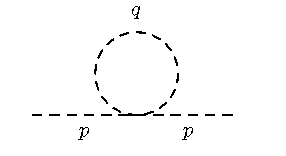
\includegraphics[scale=1]{图/phi4selfe.pdf}
\end{center}
根据上图我们可计算单圈积分：
\begin{align}
\Sigma_0&=\frac{g_0}{2}K_0(0)=\frac{ig_0}{2}\int\frac{\mathrm{d}^dq}{2(2\pi)^d(q^2-m_0^2+i\epsilon)}=\frac{ig_0}{2} I_1\notag\\
&=\frac{g\mu^\epsilon}{8\pi}\Gamma(-1+\frac{\epsilon}{2})\left(\frac{m_0^2}{4\pi}\right)^{1-\frac{\epsilon}{2}}\notag\\
&=\frac{gm_0^2}{32\pi^2}\Gamma(-1+\frac{\epsilon}{2})\left(\frac{4\pi\mu^2}{m_0^2}\right)^{\frac{\epsilon}{2}}
\end{align}
此时，我们对$\Gamma$函数作洛朗级数展开\footnote{$\Gamma$函数绕$x=0$领域洛朗级数展开：\[\Gamma(-n+x)=\frac{(-1)^n}{n!}\left(\frac{1}{x}+1+\cdots+\frac{1}{n}-\gamma+\mathcal{O}(x)\right)\]其中$\gamma\approx0.577$为Euler-马斯刻若尼常数}，得：
\begin{equation}
\Gamma(-1+\frac{\epsilon}{2})=-\left(\frac{2}{\epsilon}+1-\gamma+\mathcal{O}(\epsilon)\right)
\end{equation}
而对于圈积分中包含无穷小量幂指数的另一部分，我们可以处理为：
\begin{align}
\left(\frac{4\pi\mu^2}{m_0^2}\right)^{\frac{\epsilon}{2}}&=\exp\Big[\frac{\epsilon}{2}\ln\left(\frac{4\pi\mu^2}{m_0^2}\right)\Big]\notag\\
&\approx1+ \frac{\epsilon}{2}\ln\left(\frac{4\pi\mu^2}{m_0^2}\right)+\mathcal{O}(\epsilon^2)
\end{align}
代回到自能单圈积分内，得：
\begin{equation}
\Sigma_0=-\frac{gm_0^2}{32\pi^2}\left(\frac{2}{\epsilon}+1-\gamma+\mathcal{O}(\epsilon)\right)\left(1+\frac{\epsilon}{2}\ln\left(\frac{4\pi\mu^2}{m_0^2}\right)+\mathcal{O}(\epsilon^2)\right)
\end{equation}
展开之后，再将$\epsilon$取0，这样略去高阶项$\mathcal{O}(\epsilon)$，可得：
\begin{align}
\Sigma_0&=-\frac{gm_0^2}{32\pi^2}\left(\frac{2}{\epsilon}+1-\gamma+\ln\left(\frac{4\pi\mu^2}{m_0^2}\right)\right)\notag\\
&=-\frac{gm_0^2}{32\pi^2}\left(\frac{2}{\epsilon}+\ln\left(\frac{\mu^2}{m_0^2}\right)+\ln(4\pi e^{1-\gamma})\right)
\end{align}
代入二点Green函数中，我们可得单圈自能修正后的结果：
\begin{align}
i\tilde{G}^{-1}(p^2,\mu)&=p^2-m_0^2-\Sigma_0(\mu^2)\notag\\
&=p^2-m_0^2\Big( 1-\frac{g}{16\pi^2\epsilon}-\frac{g}{32\pi^2}\left(\ln\left(\frac{\mu^2}{m_0^2}\right)+\ln(4\pi e^{1-\gamma})\right)\Big)
\label{eq:1Lm}
\end{align}

而对于顶点修正，我们有单圈图：
\begin{center}
% \begin{fmffile}{phi4loopint}
%       \begin{fmfgraph*}(120,80)
%     \fmfleft{i1,i2}
%     \fmfright{o1,o2}
%     \fmflabel{${p}_1$}{i1}
%     \fmflabel{${p}_2$}{i2}
%     \fmflabel{${p}_3$}{o1}
%     \fmflabel{${p}_4$}{o2}
%     \fmf{dashes}{i1,v1}
%     \fmf{dashes}{v1,i2}
%     \fmf{dashes}{o2,v2}
%     \fmf{dashes}{v2,o1}
%     \fmf{dashes,left,label=\(p_1+p_2-q\)}{v1,v2}
%     \fmf{dashes,right,label=\(q\)}{v1,v2}
%   \end{fmfgraph*}
% \end{fmffile}
	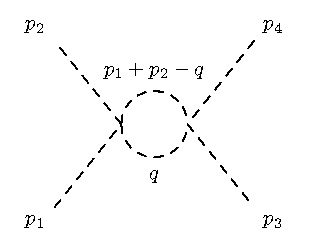
\includegraphics[scale=1]{图/phi4loopint.pdf}
\end{center}
由于我们不去人为区分四个顶点的动量，因此内线动量一共有三种不同的组合，可以用三个Mandelstam变量描述。其中一项的圈积分可表为：
\begin{align}
\tilde{\Gamma}^{(1)}(s)&=-\frac{g_0^2}{2}\int\frac{\mathrm{d}^d k}{(2\pi)^d}\frac{-1}{(k^2-m_0^2)((k-\sqrt{s})^2-m^0)}\notag\\
&=\frac{g_0^2}{2}I_{1,1}(s)=\frac{ig_0^2}{2(4\pi)^{2}}\Gamma(\frac{\epsilon}{2})\int_0^1\mathrm{d}x\Big(\frac{\Omega(x,s)}{4\pi}\Big)^{-\frac{\epsilon}{2}}\notag\\
&=\frac{ig^2\mu^\epsilon}{2(4\pi)^{2}}\Gamma(\frac{\epsilon}{2})\int_0^1\mathrm{d}x\Big(\frac{\Omega(x,s)}{4\pi\mu^2}\Big)^{-\frac{\epsilon}{2}}\\
\Omega(x,s)&=m_0^2+sx(x+1)
\end{align}
则我们可得：
\begin{align}
&\tilde{\Gamma}^{(1)}(p)=\frac{ig^2\mu^\epsilon}{2(4\pi)^{2}}\Gamma(\frac{\epsilon}{2})\int_0^1\mathrm{d}x\left(\Big(\frac{\Omega(x,s)}{4\pi\mu^2}\Big)^{-\frac{\epsilon}{2}}+\Big(\frac{\Omega(x,t)}{4\pi\mu^2}\Big)^{-\frac{\epsilon}{2}}+\Big(\frac{\Omega(x,u)}{4\pi\mu^2}\Big)^{-\frac{\epsilon}{2}}\right)\notag\\
&\approx\frac{ig^2\mu^\epsilon}{32\pi^2}\left(\frac{6}{\epsilon}-\int_0^1\mathrm{d}x\Big[\ln\Big(\frac{\Omega(x,s)}{4\pi e^{-\gamma}\mu^2}\Big)+\ln\Big(\frac{\Omega(x,t)}{4\pi e^{-\gamma}\mu^2}\Big)+\ln\Big(\frac{\Omega(x,u)}{4\pi e^{-\gamma}\mu^2}\Big)\Big]\right)
\end{align}
我们记积分项为：
\begin{equation}
F(s,m_0,\mu)=\int_0^1\mathrm{d}x\ln\Big(\frac{m_0^2+sx(x+1)}{4\pi e^{-\gamma}\mu^2}\Big)
\end{equation}
代入4点函数，我们可得其单圈修正后的结果：
\begin{equation}
\tilde{\Gamma}(g,\mu;p)=-ig\mu^\epsilon\left(1-\frac{3g}{16\pi^2\epsilon}+\frac{g}{32\pi^2}(F(s,m_0,\mu)+F(t,m_0,\mu)+F(u,m_0,\mu))\right)
\label{eq:1Lg}
\end{equation}

此时我们已经计算出了具体Green函数的单圈修正，并且已经将发散项提取了出来。为了抵消Green函数中的发散项，我们可以认为裸质量及裸耦合常数本身即为无穷大量，即
\begin{align}
&m_0^2=m_r^2 Z_m=m_r^2(1+\delta m)\notag\\
&g_0=g_r\mu^\epsilon Z_g=g_r\mu^\epsilon(1+\delta g)
\end{align}
其中$\delta m$和$\delta g$即为无穷大的抵消项。而$m_r$和$g_r$为重整化的质量及耦合常数。

若我们考虑完全修正的Green函数，即包含无穷多项高阶修正项，那么我们需要无穷多项抵消项，即为：
\begin{align}
&m_0^2=m_r^2\left(1+\sum_{k=1}^{\infty}\frac{\mathscr{M}_k(g,\mu^2)}{\epsilon^k}\right)\notag\\
&g_0=g\mu^\epsilon\left(1+\sum_{k=1}^{\infty}\frac{\mathscr{G}_k(g,\mu^2)}{\epsilon^k}\right)
\label{eq:bare}
\end{align}
然而实际计算中，我们不可能计算所有的Green函数展开项，因此我们必然只能计算到某一阶展开项为止。这样的话，裸物理量的抵消项就不需要无穷多项，只需要到我们计算的那一级次便可以抵消掉所有的发散。若我们考虑只有单圈修正，那么抵消项也只需要一级，就足够。
\begin{align}
&m_0^2=m_r^2\left(1+\frac{\mathscr{M}_1(g)}{\epsilon}\right)\notag\\
&g_0=g_r\mu^\epsilon\left(1+\frac{\mathscr{G}_1(g)}{\epsilon}\right)
\end{align}
分别代入到\eqref{eq:1Lm}式和\eqref{eq:1Lg}式中，我们可得：
\begin{align}
i\tilde{G}^{-1}(p^2,\mu)&=p^2-m_r^2\left(1+\frac{\mathscr{M}_1}{\epsilon}\right)\left[1-\frac{g}{16\pi^2\epsilon}-\frac{g}{32\pi^2}\ln\left(\frac{4\pi\mu^2 e^{1-\gamma}}{m_r^2(1+\frac{\mathscr{M}_1}{\epsilon})}\right)\right]\notag\\
&=p^2-m_r^2\left[1+\frac{\mathscr{M}_1g}{\epsilon}-\frac{g}{16\pi^2\epsilon}-\frac{g}{32\pi^2}\ln\left(\frac{4\pi\mu^2 e^{1-\gamma}}{m_r^2}\right)\right]
\end{align}
\begin{align}
\tilde{\Gamma}(g,\mu;p)&=-ig_r\mu^\epsilon\left(1+\frac{\mathscr{G}_1}{\epsilon}\right)\left(1-\frac{3g_r}{16\pi^2\epsilon}+\frac{g_r}{32\pi^2}(F(s)+F(t)+F(u))\right)\notag\\
&=-ig_r\mu^\epsilon\left(1+\frac{\mathscr{G}_1}{\epsilon}-\frac{3g_r}{16\pi^2\epsilon}+\frac{g_r}{32\pi^2}(F(s)+F(t)+F(u))\right)
\end{align}
这里对于2点函数的修正，我们略去$\mathcal{O}(g^2)$项。对于4点函数的修正，我们略去$\mathcal{O}(g^3)$项。然而我们注意到这些关于耦合常数的高阶项中是包含了更高级次的发散项的。但我们这里将其忽略，是因为我们只截取到了一级修正项。而那些更高级次的发散项则需要我们引入下一级次的修正项和重整化抵消项才能被完全消去。但同时，我们也会引入再高一级的发散。如此往复，只有我们计算出全部的修正项，才能完全抵消掉所有的发散。但显然我们做不到，因此我们对于特定级次的修正项，其发散项也只能被一级一级地消去。

那么对于最小差值方案来说，我们应该用尽可能简短的抵消项来抵消发散项，由上式解得：
\begin{equation}
\mathscr{M}_1=\frac{g}{16\pi^2},\qquad\mathscr{G}_1=\frac{3g_r}{16\pi^2}
\end{equation}
即得裸质量及裸耦合常数：
\begin{align}
&m_0^2=m^2\left(1+\frac{g}{16\pi^2\epsilon}\right)\notag\\
&g_0=g_r\mu^\epsilon\left(1+\frac{3g_r}{16\pi^2\epsilon}\right)
\end{align}

然而这种最小差值方案计算得出的物理量中往往包含一些有限的常数项，例如$\ln(4\pi e^{\gamma})$。为了使得物理结果更加简洁，我们又有另一种最小差值方案。即将这些有限常数项也放到裸物理量中，称为$\overline{\text{MS}}$方案。其裸质量和裸耦合常数为：
\begin{align}
&m_0^2=m_{\overline{\text{MS}}}^2\left(1+\frac{g}{16\pi^2\epsilon}+\frac{g}{32\pi^2}\ln(4\pi e^{1-\gamma})\right)\notag\\
&g_0=g_r\mu^\epsilon\left(1+\frac{3g_r}{16\pi^2\epsilon}+\frac{3g_r}{32\pi^2}\ln(4\pi e^{-\gamma})\right)
\end{align}

这时再代入到单圈修正的自能中，抵消掉5无穷大项，并让正规化因子$\epsilon$回归到0，可得$\overline{\text{MS}}$重整化后的Green函数：
\begin{gather}
G(p^2,\mu)=\frac{i}{\displaystyle{p^2-m_{\overline{\text{MS}}}^2\left(1-\frac{g}{32\pi^2}\ln\left(\frac{\mu^2}{m_{\overline{\text{MS}}}^2}\right)\right)}}\\
\tilde{\Gamma}(g,\mu;p)=-ig_r\Big(1+\frac{g_r}{32\pi^2}\Big[3\ln\left(\frac{m^2}{\mu^2}\right)-6+f(m,s)+f(m,t)+f(m,u)\Big]\Big)\\
f(m,s)=2\sqrt{\frac{4m^2-s}{s}}\arctan\left(\sqrt{\frac{s}{4m^2-s}}\right)\notag
\end{gather}
由单圈修正后的2点Green函数我们可以看出，传播子中的质量项实际上变为了：
\begin{align}
    m^2&=m_{\overline{\text{MS}}}^2\left(1-\frac{g}{32\pi^2}\ln\left(\frac{\mu^2}{m_{\overline{\text{MS}}}^2}\right)\right)\notag\\
    &=m_{\overline{\text{MS}}}^2+\Sigma_r(\mu)
\end{align}
%这使得当我们使用MS或$\overline{\text{MS}}$方法时，我们实际上考虑的粒子质量是依赖于重整化能标的选择，而这样的质量则称之为跑动质量。
此时我们注意到，粒子的自能项依赖于能标的取值。然而实际情况中我们考虑的测量到的粒子质量应为粒子的静止质量，是不依赖于任何外部条件的，也称为物理质量。因此我们将粒子的物理质量定义为粒子传播子的极点，而当粒子动量恰好为传播子极点时，即处于在壳状态，也即静止状态。而在考虑传播子的重整化之后，粒子的质量项可以分为树图贡献以及自能部分，但是加起来的总和恒为传播子的极点，即物理质量。因此当自能部分依赖于能标时，树图质量也依赖于能标，则此时的树图质量$m_{\overline{\text{MS}}}$称为$\overline{\text{MS}}$质量。
\subsection{在壳重整化方案}
然而在实际计算当中，我们实际上无法通过计算得出粒子的$\overline{\text{MS}}$质量，只能通过用测量的物理质量及粒子自能计算反过来拟合出$\overline{\text{MS}}$质量。这样的计算方案非常不方便，而且也难以准确。因此我们考虑另一种重整化方案，使得树图层面的粒子质量就直接是物理质量，即粒子自能恰好消为0，称为\emph{在壳重整化方案}。

%我们希望将粒子质量当作常数。因此为了使粒子质量不受重整化能标影响，我们可以考虑另一种重整化方案

我们考虑粒子传播子存在极点$m_\text{pole}$，也称为极点质量。由于极点质量为粒子的静止质量，我们可以考虑能标在粒子静止质量时的粒子自能，则有：
\begin{equation}
    m^2_\text{pole}=m^2+\Sigma_r(m_\text{pole})
\end{equation}
%=m_0^2+\Sigma_0(m_\text{pole})
而同时，2点Green函数还处于复空间中的极点，则有留数定理：
\begin{equation}
    i=\lim_{p\rightarrow m_\text{pole}}(p^2-m^2_\text{pole})\frac{i}{p^2-m^2-\Sigma_r(m_\text{pole})-(p^2-m^2_\text{pole})\frac{\mathrm{d}\Sigma_r(p^2)}{\mathrm{d}p^2}|_{p^2=m^2_\text{pole}}+\cdots}
\end{equation}
%\begin{equation}
 %   i=\lim_{p\rightarrow m_\text{pole}}(\slashed{p}-m_\text{pole})\frac{i}{\slashed{p}-m_r-\Sigma_r(m_\text{pole})-(\slashed{p}-m_\text{pole})\frac{\mathrm{d}\Sigma_r(\slashed{p})}{\mathrm{d}\slashed{p}}|_{\slashed{p}=m_\text{pole}}+\cdots}
%\end{equation}
那么推导得：
\begin{equation}
    \frac{\mathrm{d}\Sigma_r(p^2)}{\mathrm{d}p^2}\Big|_{p^2=m^2_\text{pole}}=0
\end{equation}
%\begin{equation}
%    \frac{\mathrm{d}\Sigma_r(\slashed{p})}{\mathrm{d}\slashed{p}}\Big|_{\slashed{p}=m_\text{pole}}=0
%\end{equation}
由于我们希望最终的树图层面的质量被固定为极点质量$m=m_\text{pole}$，并结合上述关系，我们可得在壳重整化的两个条件：
\begin{equation}
    \Sigma_r(m_\text{pole})=0,\qquad\frac{\mathrm{d}\Sigma_r(p^2)}{\mathrm{d}p^2}\Big|_{p^2=m^2_\text{pole}}=0
\end{equation}
对于Fermion而言，则其在壳重整化的条件为：
\begin{equation}
    \Sigma_r(m_\text{pole})=0,\qquad\frac{\mathrm{d}\Sigma_r(\slashed{p})}{\mathrm{d}\slashed{p}}\Big|_{\slashed{p}=m_\text{pole}}=0
\end{equation}
因此在壳重整化方案的最终结果实际依赖于自能的形式。对于纯标量场而言，质量重整化并不会影响到耦合常数的重整化，此时可以对场和耦合常数使用不同的重整化方案。但是对于更加复杂的场及系统而言，当质量采用在壳重整化方案时，场及耦合常数的重整化也会受到影响，重整化方案的选用也要视具体情况决定。


\section{重整化群}
上一节中我们已经得到了重整化后的Green函数，即物理可观测量。虽然我们已经得到了具有物理意义的结果，然而我们可以看到，这些物理量结果都依赖于能标参数$\mu$。那么这意味着，实际上我们所认为的物理常量，质量$m$、耦合常数$g$是会随着能标的改变而变化的。

同时，这也隐含了我们的理论实际上具有一定的能标局域性，只能描述一个特定能标下的物理规律，而一旦能标发生巨大的变化，那么原来的理论很有可能则不再适用。然而我们并非完全无法通过现有能标下的理论来了解其它能标下的规律，这样一种将不同能标下的理论联系起来的方法则是建立起一个\emph{重整化群}。

对于一个可重整化的理论，我们知道有裸Lagrangian$\mathcal{L}_0$以及裸场$\phi_0$，裸质量$m_0$和裸耦合常数$g_0$，并且我们有裸物理量与重整化物理量的关系：
\begin{equation}
\phi_0=\phi Z^{\frac{1}{2}}_\phi,\qquad m^2_0=m^2 Z_m,\qquad g_0=g Z_g
\end{equation}
那么通过裸Lagrangian导出的裸Green函数与重整化后的物理Green函数之间便有关系：
\begin{equation}
G^{(n)}_0(p_i,g_0,m_0;\epsilon)=Z_\phi^{\frac{n}{2}}G^{(n)}(p_i,g,m,\mu;\epsilon)
\end{equation}
我们可以知道，实际上重整化的过程我们可以看成是将裸的物理量进行“等比例”放缩，而这个放缩的比例标度则是能标$\mu$。那么当这个能标$\mu$跑遍所有正实数，就可以得到一系列缩放比例不同的重整化Green函数。所有的这些重整化Green函数则构成了一个重整化群。

\subsection{重整化群方程}
那么我们可以对上式两侧对能标求导，左边的裸Green函数本身是独立于能标的量，求导结果则必然为0：
\begin{equation}
0=\mu\frac{\mathrm{d}}{\mathrm{d}\mu}G^{(n)}_0(p_i,g_0,m_0;\epsilon)=\mu\frac{\mathrm{d}}{\mathrm{d}\mu}\left[Z_\phi^{\frac{n}{2}}G^{(n)}(p_i,g,m,\mu;\epsilon)\right]
\end{equation}
而右边的物理Green函数则依赖于或隐含了能标，则利用链式法则可得：
\begin{equation}
\left[\mu\frac{\mathrm{d}}{\mathrm{d}\mu}+\mu\frac{\partial g}{\partial\mu}\frac{\partial}{\partial g}+\mu\frac{\partial m}{\partial\mu}\frac{\partial}{\partial m}+\frac{n}{2}\mu\frac{\partial\ln Z_\phi}{\partial\mu}\right]G^{(n)}(p_i,g,m,\mu;\epsilon)=0
\end{equation}
从上式中我们可以定义以下无量纲函数：
\begin{align}
\beta(g,m,\mu)&=\mu\frac{\partial g}{\partial\mu},\notag\\
\gamma_m(g,m,\mu)&=\frac{\mu}{m}\frac{\partial m}{\partial\mu},\notag\\
\gamma_\phi(g,m,\mu)&=\mu\frac{\partial\ln Z_\phi}{\partial\mu}
\end{align}
那么我们可以有：
\begin{equation}
\left[\mu\frac{\mathrm{d}}{\mathrm{d}\mu}+\beta\frac{\partial}{\partial g}+\gamma_m\frac{\partial}{\partial m}+\frac{n}{2}\gamma_\phi\right]G^{(n)}(p_i,g,m,\mu;\epsilon)=0
\end{equation}
即所谓\emph{重整化群方程}，或者也称为Callan-Symanzik方程。

该方程联系了重整化群中的所有元素，即各种不同能标的重整化Green函数之间的连接关系。而其中的函数$\beta(g)$和$\gamma_m(g)$则展示了耦合常数和质量是如何随能标变化而变化的。

\subsection{$\beta$-函数及反常量纲}
由裸耦合常数的定义\eqref{eq:bare}，我们可对裸耦合常数作全微分得：
\begin{equation}
0=\mu\frac{\mathrm{d} g_0}{\mathrm{d}\mu}=\mu\frac{\mathrm{d} g}{\mathrm{d}\mu}\left(1+\sum_k\frac{\mathscr{G}_k}{\epsilon^k}\right)+\epsilon g\left(1+\sum_k\frac{\mathscr{G}_k}{\epsilon^k}\right)+g\mu\frac{\mathrm{d} g}{\mathrm{d}\mu}\sum_k\frac{1}{\epsilon^k}\frac{\partial\mathscr{G}_k}{\partial g}
\label{eq:beta1}
\end{equation}
得：
\begin{equation}
\mu\frac{\mathrm{d} g}{\mathrm{d}\mu}=-\epsilon g\left(\frac{1+\sum_k\frac{\mathscr{G}_k}{\epsilon^k}}{1+\sum_k\frac{\mathscr{G}_k}{\epsilon^k}+g\sum_k\frac{1}{\epsilon^k}\frac{\partial\mathscr{G}_k}{\partial g}}\right)
\end{equation}
对右式分母以$g$为小量作展开，可得：
\begin{equation}
\mu\frac{\mathrm{d} g}{\mathrm{d}\mu}=-\epsilon g\left(1-g\sum_k\frac{1}{\epsilon^k}\frac{\partial\mathscr{G}_k}{\partial g}+\mathcal{O}(g^2)+\cdots\right)
\end{equation}
由于重整化中的发散项是以一级一级逐阶抵消，所以如果我们只考虑$g$的一阶项，略去二阶以上的项，我们就只考虑一级发散$k=1$，最后令$\epsilon\rightarrow0$，我们便可得此时的$\beta$-函数:
\begin{equation}
\beta(g)=g^2\frac{\partial\mathscr{G}_1}{\partial g}\label{eq:beta2}
\end{equation}
此时对耦合常数的全微分可以表示为：
\begin{equation}
\mu\frac{\mathrm{d} g}{\mathrm{d}\mu}=-\epsilon g+\beta(g)\label{eq:beta3}
\end{equation}
这时我们又可以将次全微分代回到\eqref{eq:beta1}式中，可得：
\begin{equation}
\beta+\beta\sum_k\frac{\mathscr{G}_k}{\epsilon^k}+\beta g\sum_k\frac{1}{\epsilon^k}\frac{\partial\mathscr{G}_k}{\partial g}=g^2\sum_k\frac{1}{\epsilon^{k-1}}\frac{\partial\mathscr{G}_k}{\partial g}
\end{equation}
由于不同$k$的\(\frac{1}{\epsilon^k}\)之间相互独立，因此在此式中当$k=1$时，我们必定得到\eqref{eq:beta2}。由此可见\eqref{eq:beta2}对于任意级次的发散都成立，即$\beta$-函数恒为裸耦合质量中单极点的留数。那么对于任意$k$，则需要满足关系：
\begin{equation}
g^2\frac{\partial\mathscr{G}_{k+1}}{\partial g}=\beta(g)\left(\mathscr{G}_k+g\frac{\partial\mathscr{G}_k}{\partial g}\right)
\end{equation}

同样，由\eqref{eq:bare}式中的裸质量，我们可以作全微分得：
\begin{equation}
0=\frac{\mu}{m}\frac{\mathrm{d}m_0^2}{\mathrm{d}\mu}=2\mu\frac{\mathrm{d}m}{\mathrm{d}\mu}+m\mu\frac{\mathrm{d}g}{\mathrm{d}\mu}\sum_k\frac{1}{\epsilon^k}\frac{\partial\mathscr{M}_k}{\partial g}
\end{equation}
其中代入\eqref{eq:beta3}式，可得：
\begin{equation}
2\mu\frac{\mathrm{d}m}{\mathrm{d}\mu}-mg\sum_k\frac{1}{\epsilon^{k-1}}\frac{\partial\mathscr{M}_k}{\partial g}+\beta(g)m\sum_k\frac{1}{\epsilon^k}\frac{\partial\mathscr{M}_k}{\partial g}=0
\end{equation}
由$k=1$次项，我们可得：
\begin{equation}
\gamma_m=\frac{\mu}{m}\frac{\partial m}{\partial\mu}=\frac{g}{2}\frac{\partial\mathscr{M}_1}{\partial g}
\end{equation}
$\gamma_m$即称为反常量纲。同时对任意次$k$我们也有关系：
\begin{equation}
\beta(g)\frac{\partial\mathscr{M}_k}{\partial g}=g\frac{\partial\mathscr{M}_{k+1}}{\partial g}
\end{equation}


对于之前作为例子的实标量$\phi^4$理论，我们可得单圈$\beta$-函数和反常量纲：
\begin{align}
\beta(g)=\frac{3g^2}{16\pi^2}\notag\\
\gamma_m(g)=\frac{g}{32\pi^2}
\end{align}
对于$\beta$-函数，我们可以考虑对其积分，先写为：
\begin{equation}
    \frac{\mathrm{d}g}{g^2}=\frac{3}{16\pi^2}\mathrm{d}\ln\mu
\end{equation}
作定积分得：
\begin{equation}
    \frac{1}{g}-\frac{1}{g_\Lambda}=-\frac{3}{16\pi^2}\ln\frac{\mu}{\Lambda}
\end{equation}
其中$\Lambda$为参考能标，而$g_\Lambda$为参考能标下的耦合常数。因此我们可得跑动耦合常数依赖于能标的关系：
\begin{equation}
    g(\mu)=\frac{g_\Lambda}{1-\frac{3g_\Lambda}{16\pi^2}\ln\frac{\mu}{\Lambda}}
\end{equation}

\subsubsection*{$\beta$-函数渐近性质}
我们已经知道$\beta$-函数描述了耦合常数随能标变化而变化的性质，但同时我们也知道，耦合常数在我们动力学微扰展开中至关重要。我们之所以能进行微扰展开，是因为我们的耦合常数一般小于1，这样才能保证越高阶的展开项越收敛。然而耦合常数会变化的这一性质意味着，存在着使得耦合常数变化到大于1的可能性。在这时，我们微扰展开的方法将不再适用，Feynman图等等计算手段也受到了限制。因此讨论$\beta$-函数在何时使得耦合常数大于1是十分重要的。
\begin{itemize}
	\item 当$\beta(g)>0$时，意味着耦合常数$g$则会随着能标$\mu$的增大而增大。最终某个能标极大的区域，耦合常数将会增大到超过1。此时微扰理论不再适用，而对应的能标即称为\emph{朗道极点}。
	\item 当$\beta(g)<0$时，则意味着耦合常数$g$随着能标降低而增大。这时则有可能在某个低能标的区域耦合常数会超过1。而另一方面，当能标极高的时候，则耦合常数变得极小，近乎于退耦合。这样的现象则称为\emph{渐近自由}。
\end{itemize}

除此之外，$\beta(g_{\star})=0$时则是另一种情况，称之为\emph{不动点}。那么$\beta$-函数则可以绕不动点领域展开：
\begin{equation}
\beta(g)=\mu\frac{\partial g}{\partial\mu}=(g-g_{\star})\beta'(g_{\star})+\cdots
\end{equation}
解微分方程可得：
\begin{equation}
g=g_{\star}+g_0e^{\beta'(g_{\star})\ln\frac{\mu}{\mu_0}}
\end{equation}
其中$\mu_0$为参考能标。

那么如果不动点处的$\beta$-函数的导数$\beta'(g_\star)<0$，则在能标$\mu\rightarrow\infty$处，耦合常数趋近于不动点。这样的不动点称之为紫外不动点。

而当$\beta'(g_\star)>0$时，耦合常数则在能标$\mu\rightarrow0$处趋近于不动点。即称之为红外不动点。
\epigraphhead[650]{}
\part{规范场论}
\section*{规范对称性-内禀局域对称性}
我们考虑场的内禀局域变换，即变换参数依赖于时空位置：
\begin{equation}
	\psi(x)\rightarrow U(x)\psi(x) \tag{P.2.1}
\end{equation}
此时Lagrangian$\mathscr{L}_0$无法在此变换下保持不变,即表现为场沿某方向$n^\mu$的时空平移同时引起了内禀对称变换的变化，使得其导数$n^\mu\partial_\mu\psi$不为简单的几何表述。为了获得简单几何表述的导数形式，我们在变换的流形上定义平行移动：
\begin{equation}
	\Gamma(n)^y_x : \psi(x)\rightarrow\psi(y) \tag{P.2.2}
\end{equation}
即可将场从$x$点平行移动到$y$点。我们则可以定义其协变导数：
\begin{equation}
	n^\mu D_\mu\psi=\lim_{\epsilon\rightarrow 0}\frac{\psi(x+\epsilon n)-\Gamma(n)^{x+\epsilon n}_x\psi(x)}{\epsilon}\tag{P.2.3}
	\label{co-d}
\end{equation}
此时我们在Lagrangian中修改微分算符$\partial_\mu$为协变导数$D_\mu$，使得：
\begin{equation}
	D_\mu\Big( U(x)\psi(x)\Big)=U(x)\Big(D_\mu \psi(x)\Big)\tag{P.2.4}
\end{equation}
即表为协变导数同时具有变换：
\begin{equation}
	D_\mu\rightarrow U(x)D_\mu U^\dagger(x)\tag{P.2.5}
\end{equation}
此时修改后的Lagrangian动能项才能在局域变换下保持不变，即具有局域对称性：
\begin{equation}
	\mathscr{L}_0=\bar{\psi}(x)i\gamma^\mu D_\mu\psi(x)\tag{P.2.6}
\end{equation}
考虑在极小时空位移下的平行移动，我们可以将其展开为：
\begin{equation}
	\Gamma(n)^{x+\epsilon n}_x = 1 + i g\,\epsilon\, n^\mu A_\mu(x) +\mathcal{O}(\epsilon^2)\tag{P.2.7}
\end{equation}
其中$A_\mu$为平行移动的联络，而无量纲参数$g$则反映了平行移动的变化强度。代入\eqref{co-d}中，我们可得：
\begin{equation}
	D_\mu=\partial_\mu-ig A_\mu(x)\tag{P.2.8}
\end{equation}
其中引入的联络$A_\mu(x)$同时也是一个矢量场
而协变导数满足Jacobi恒等式：
\begin{equation}
	[D_\mu,[D_\nu,D_\rho]]+[D_\nu,[D_\rho,D_\mu]]+[D_\rho,[D_\mu,D_\nu]]=0\tag{P.2.9}
\end{equation}
对于协变导数，我们定义为局域对称性变换下的伴随表示，有：
\begin{align}
	D'_\mu&=\partial_\mu-ig A'_\mu(x)\notag\\
	&=U(x)D_\mu U^\dagger(x)=U(x)\Big(\partial_\mu-ig A_\mu(x)\Big)U^\dagger(x)\notag\\
	&=\partial_\mu+U(x)\Big(\partial_\mu U^\dagger(x)\Big)-igU(x)A_\mu(x)U^\dagger(x)\tag{P.2.10}
\end{align}
由此我们可知矢量场$A_\mu(x)$在局域对称变换下有如下变换形式：
\begin{equation}
	A_\mu(x)\rightarrow A'_\mu(x)=U(x)A_\mu(x)U^\dagger(x)+\frac{i}{g}U(x)\Big(\partial_\mu U^\dagger(x)\Big)\tag{P.2.11}
	\label{eq:gaugetr}
\end{equation}
由于矢量场本身允许具有内禀的规范对称性，场在规范空间中变换不改变最终描述的场本身。因此$A_\mu(x)$的变换可以看成其规范对称性变换，而我们也将$A_\mu(x)$称为规范场。

对于场强张量$F_{\mu\nu}$，可构建为规范群流形上的曲率张量，即：
\begin{equation}
	[D_\mu,D_\nu]=-ig F_{\mu\nu}\tag{P.2.12}
\end{equation}
则我们可得：
\begin{equation}
	F_{\mu\nu}(x)=\partial_\mu A_\nu(x)-\partial_\nu A_\mu(x)-ig[A_\mu(x),A_\nu(x)]\tag{P.2.13}
\end{equation}
场强$F_{\mu\nu}$具有反对称性，并且满足Bianchi恒等式：
\begin{equation}
	D_{\mu}F_{\nu\rho}+D_\nu F_{\rho\mu}+D_\rho F_{\mu\nu}=0\tag{P.2.14}
\end{equation}
我们还可以定义，场强$F_{\mu\nu}$的对偶：
\begin{equation}
\tilde{F}_{\mu\nu}=\frac{1}{2}\epsilon_{\mu\nu\rho\sigma}F^{\rho\sigma}\tag{P.2.15}
\end{equation}
我们可以将Bianchi恒等式写为：
\begin{equation}
D^\mu\tilde{F}_{\mu\nu}=0\tag{P.2.16}
\end{equation}
\chapter{量子电动力学-Abliean规范场理论}
\section{电磁相互作用与其费曼规则}
对于电磁场而言，$A_\mu$并不具有更高的内禀自由度，则参与电磁相互作用的费米子场将会具有内禀局域U(1)对称性，即：
\begin{equation}
	U(x)=e^{i\alpha(x)}
\end{equation}
而对应的耦合常数$g=-e$。此时协变导数为：
\begin{equation}
	D_\mu=\partial_\mu+ieA_\mu
\end{equation}
电磁场的规范变换则为：
\begin{equation}
	A_\mu\rightarrow A_\mu-\frac{1}{e}\partial_\mu\alpha(x)
\end{equation}
同样，此时电磁场$A_\mu$之间相互对易，即代表电磁场之间互不相干，我们又称电磁场为Abliean规范场。由此可得电磁场张量：
\begin{equation}
	F_{\mu\nu}=\partial_\mu A_\nu-\partial_\mu A_\nu
\end{equation}
则我们可得电磁场以及参与电磁相互作用的费米子场的总Lagrangian:
\begin{align}
	\mathscr{L}_{\text{QED}}&=\bar{\psi}(i\slashed{D}-m)\psi-\frac{1}{4}F_{\mu\nu}F^{\mu\nu}\notag\\
	&=i\bar{\psi}\slashed{\partial}\psi-m\bar{\psi}\psi-\frac{1}{4}F_{\mu\nu}F^{\mu\nu}-e\bar{\psi}\slashed{A}\psi
\end{align}
其中$e\bar{\psi}\slashed{A}\psi$即为费米子与电磁场的相互作用项。
以此我们可得运动方程：
\begin{align}
(i\slashed{\partial}-m)\psi=e \slashed{A}\psi\notag\\
\partial_\mu F^{\mu\nu}=e\bar{\psi}\gamma^\nu\psi
\end{align}
由此我们可得守恒流$J^\mu$，也即电流密度：
\begin{equation}
J^\mu=e\bar{\psi}\gamma^\mu\psi
\end{equation}

同时我们可构造广义动量：
\begin{equation}
\pi=\frac{\partial\mathscr{L}}{\partial\dot{\psi}}=i\psi^\dagger,\qquad\pi^\mu=\frac{\partial\mathscr{L}}{\partial\dot{A}_\mu}=F^{\mu0}-\eta^{\mu0}(\partial^\nu A_\nu)
\end{equation}
其中电磁场引用费曼规范，则我们可得哈密顿量：
\begin{equation}
\mathscr{H}=\bar{\psi}(-i\gamma^i\partial_i+m)\psi+\frac{1}{2}(\partial_i A_\mu\partial^i A^\mu-\dot{A}_\mu\dot{A}^\mu)+e\bar{\psi}\gamma^\mu\psi A_\mu
\end{equation}
而对于时空平移对称性的守恒流，即为能动张量：
\begin{equation}
T^{\mu\nu}=i\bar{\psi}\gamma^\mu\partial^\nu\psi-F^{\mu\rho}\partial^\nu A_\rho-(\partial^\rho A_\rho)\partial^\nu A^\mu-\eta^{\mu\nu}\mathscr{L}
\end{equation}
而QED的格林函数生成泛函则为：
\begin{equation}
Z[J^\mu,\bar{\eta},\eta]=\int\mathcal{D}A_\mu\mathcal{D}\bar{\psi}\mathcal{D}\psi\;e^{i\int\mathrm{d}x(\mathscr{L}_{\text{QED}}+A_\mu J^\mu+\bar{\psi}\eta+\bar{\eta}\psi)}
\end{equation}
在洛伦兹规范下 从运动方程中我们可以分别求解得带电费米子场和电磁场：
\begin{equation}
\psi(x)=\int\frac{\mathrm{d}\boldsymbol{p}}{(2\pi)^{3/2}\sqrt{2E(\boldsymbol{p})}}\sum^2_{r=1}\Big(b_r(\boldsymbol{p})u^r(\boldsymbol{p})e^{-ipk}+d^\dagger_r(\boldsymbol{p})v^r(\boldsymbol{p})e^{ikx}\Big)
\end{equation}
\begin{equation}
A_\mu(x)=\int\frac{\mathrm{d}\boldsymbol{k}}{(2\pi)^{3/2}\sqrt{2\omega(\boldsymbol{k})}}\sum^2_{r=1}\Big(\varepsilon^r_\mu(\boldsymbol{k}) a_r(\boldsymbol{k})e^{-ik}+\varepsilon^r_\mu(\boldsymbol{k})a^\dagger_r(\boldsymbol{k})e^{ikx}\Big)
\end{equation}

因此对于量子电动力学，我们可以根据场论的动力学理论计算出其费曼规则为：
\begin{itemize}
\item 传播子
\begin{figure}[H]
	\begin{minipage}{.5\textwidth}
		\centering
		\caption*{费米子传播子}
		\begin{equation*}
			\wick{\c1{\psi}(x_1)\c1{\bar{\psi}}(x_2)}=\frac{i}{\slashed{p}-m+i\epsilon}
		\end{equation*}
		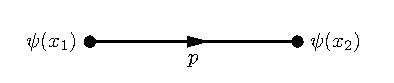
\includegraphics[width=.7\textwidth]{图/e-propa.pdf}
  %   \begin{fmffile}{e-propa}
  %             \begin{fmfgraph*}(100,40)
  %      \fmfleft{i}
  %      \fmfright{o}
  %      \fmflabel{$\psi(x_2)$}{o}
  %      \fmflabel{$\psi(x_1)$}{i}
  %      \fmfv{d.sh=circle,d.f=1,d.si=5pt}{i}
  %      \fmfv{d.sh=circle,d.f=1,d.si=5pt}{o}
  %      \fmf{fermion,tension=1,label=$k$}{i,o}
  %   \end{fmfgraph*}
  % \end{fmffile}
	\end{minipage}
	\begin{minipage}{.5\textwidth}
		\centering
				\caption*{光子传播子}
		\begin{equation*}
			\wick{\c1{A_\mu}(x_1)\c1{A_\nu}(x_2)}=\frac{-i\eta_{\mu\nu}}{k^2+i\epsilon}
		\end{equation*}
  % \begin{fmffile}{gam-propa}
  %             \begin{fmfgraph*}(100,40)
  %      \fmfleft{i}
  %      \fmfright{o}
  %      \fmflabel{$A_\nu(x_2)$}{o}
  %      \fmflabel{$A_\mu(x_1)$}{i}
  %      \fmfv{d.sh=circle,d.f=1,d.si=5pt}{i}
  %      \fmfv{d.sh=circle,d.f=1,d.si=5pt}{o}
  %      \fmf{boson,tension=1,label=$k$}{i,o}
  %   \end{fmfgraph*}
  % \end{fmffile}
		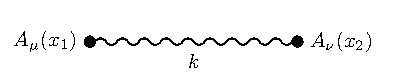
\includegraphics[width=.7\textwidth]{图/gam-propa.pdf}
	\end{minipage}
\end{figure}
\end{itemize}
\begin{itemize}
\item 顶点
\begin{figure}[H]
\begin{minipage}{.5\textwidth}
	\vspace{-20pt}
	\hspace{2cm}电磁相互作用顶点
\[\qquad\qquad\tilde{\Gamma}[A_\mu(x_1),\psi(x_2),\bar{\psi}(x_3)]\;=\;-ie\gamma^\mu\]
\end{minipage}
\begin{minipage}{.5\textwidth}
	\centering
%          \begin{fmffile}{qedint}
% \begin{fmfgraph*}(100,100)
%     \fmfleft{i1,i2}
%     \fmfright{i3}
%     \fmflabel{$\Bar{\psi} (x_3)$}{i2}
%     \fmflabel{$\psi (x_2)$}{i1}
%     \fmflabel{$A_\mu (x_1)$}{i3}
%     \fmf{fermion,label=$p$}{i1,v}
%     \fmf{fermion,label=$q$}{v,i2}
%     \fmf{boson,label=$k$}{v,i3}
%     \fmfv{d.sh=circle,d.f=1,d.si=5pt}{i1}
%     \fmfv{d.sh=circle,d.f=1,d.si=5pt}{i2}
%     \fmfv{d.sh=circle,d.f=1,d.si=5pt}{i3}
%   \end{fmfgraph*}
% \end{fmffile}
	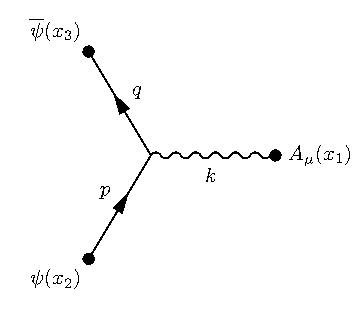
\includegraphics[width=.7\textwidth]{图/qedint.pdf}
\end{minipage}
\end{figure}
\item 外线
\subitem 入射费米子：\hspace{2cm}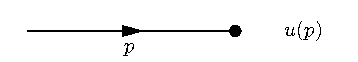
\includegraphics[scale=1]{图/in-e.pdf}%\hspace{1cm}\(u(\boldsymbol{p})\)
\vspace{5pt}
\subitem 出射费米子：\hspace{2cm}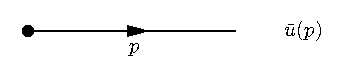
\includegraphics[scale=1]{图/out-e.pdf}%\hspace{1cm}\(\bar{u}(\boldsymbol{p})\)
\vspace{5pt}
\subitem 入射反费米子：\hspace{1.7cm}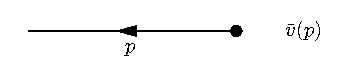
\includegraphics[scale=1]{图/in-pos.pdf}%\hspace{1cm}\(\bar{v}(\boldsymbol{p})\)
\vspace{5pt}
\subitem
出射反费米子：\hspace{1.7cm}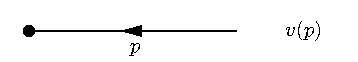
\includegraphics[scale=1]{图/out-pos.pdf}%\hspace{1cm}\(v(\boldsymbol{p})\)
\vspace{5pt}
\subitem 入射光子：\hspace{2.4cm}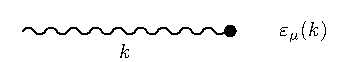
\includegraphics[scale=1]{图/in-gam.pdf}%\hspace{1cm}\(\varepsilon_\mu(\boldsymbol{k})\)
\vspace{5pt}
\subitem
出射光子：\hspace{2.4cm}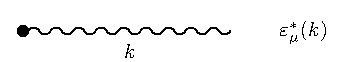
\includegraphics[scale=1]{图/out-gam.pdf}%\hspace{1cm}\(\varepsilon^*_\mu(\boldsymbol{k})\)
\end{itemize}
\section{Ward-高桥恒等式}
我们知道，对规范不变的QED系统来说，整个系统具有规范不变性，即各场在如下变换中保持运动方程不变：
\begin{equation}
	\begin{split}
		\delta A_\mu&=-\frac{1}{e}\partial_\mu\alpha(x)\\
		\delta \psi&=i\alpha(x)\psi\\
		\delta \bar{\psi}&=-i\alpha(x)\bar{\psi}
	\end{split}
\end{equation}
然而当我们考虑固定规范时，规范约束项则破坏了规范对称性。例如在$R_\xi$规范下，规范变换则会引起规范约束项产生额外的项。但是我们知道对于带电粒子的规范对称性而言，其不仅仅是一内禀的属性，更隐含了电荷守恒，因此在考虑电磁场与费米子场耦合时，不能简单的破坏掉规范对称性。

由此我们可以考虑有外源场情形下的QED，那么格林函数生成泛函则为：
\begin{equation}
	Z[J^\mu,\bar{\eta},\eta]=\int\mathcal{D}A_\mu\mathcal{D}\bar{\psi}\mathcal{D}\psi\exp\Big\{i\int\mathrm{d}x\Big(\bar{\psi}(i\slashed{D}-m)\psi-\frac{1}{4}F_{\mu\nu} F^{\mu\nu}-\frac{1}{2\xi}(\partial_\mu A^\mu)^2+A_\mu J^\mu+\bar{\psi}\eta+\bar{\eta}\psi\Big)\Big\}
\end{equation}
那么对于此时指数内的作用量，在规范变换下我们仍要保持其不变。不考虑前两项规范不变项，那么规范固定项及外源项在规范变换下产生的部分则需要为0，即：
\begin{equation}
	\int\mathrm{d}x\left[\frac{1}{\xi e}(\partial^\nu A_\nu)\partial^\mu\partial_\mu\alpha-\frac{1}{e}J^\mu\partial_\mu\alpha+i\alpha(\bar{\eta}\psi-\bar{\psi}\eta)\right]=0
\end{equation}
此时，我们需要考虑外源$J^\mu$在该系统下的表达形式，我们便可以考虑有效作用量。由\eqref{eq:effact}式，我们可得有效作用量：
\begin{equation}
	\Gamma[A_\mu,\psi,\bar{\psi}]=-i\ln Z[J^\mu,\bar{\eta},\eta]-\int\mathrm{d}x(A_\mu J^\mu+\bar{\eta}\psi+\bar{\psi}\eta)
\end{equation}
那么我们可得：
\begin{equation}
	\frac{\delta\Gamma}{\delta A_\mu}=-J^\mu,\qquad\frac{\delta\Gamma}{\delta\psi}=\bar{\eta},\qquad\frac{\delta\Gamma}{\delta\bar{\psi}}=-\eta
\end{equation}
那么将外源的表达式代入到对称性条件，即可的：
% \begin{small}
	\begin{equation}
		\int\mathrm{d}x\left[\frac{\delta\Gamma}{\delta A_\mu(x)}\partial_\mu\alpha(x)+\frac{\partial^\nu A_\nu(x)}{\xi }\partial^\mu\partial_\mu\alpha(x)+i\alpha(x)(\frac{\delta\Gamma}{\delta\psi(x)}\psi(x)+\bar{\psi}(x)\frac{\delta\Gamma}{\delta\bar{\psi(x)}})\right]=0
		\label{eq:wardori}
	\end{equation}
% \end{small}
这便是最原始形式的Ward-高桥恒等式。

由之前对有效作用量及外源场的讨论，有效作用量可表为：
\begin{multline}
	\Gamma=\int\mathrm{d}x\Big[\int\mathrm{d}y\Big(	\frac{1}{2}A_\mu(x)\bar{\Gamma}^{\mu\nu}_{A}(x,y)A_\nu(y)+\bar{\psi}(x)\bar{\Gamma}_{\psi}(x,y)\psi(y)\Big)	\\	+\int\mathrm{d}y\mathrm{d}z\;\bar{\psi}(x)A_\mu(y)\bar{\Gamma}^\mu_3(x,y,z)\psi(z)+\cdots\Big]
\end{multline}
我们易得有效作用量泛函导数：
\begin{align}
	\frac{\delta \Gamma}{\delta A_\mu(x)}&=\int\mathrm{d}y\; \bar{\Gamma}^{\mu\nu}_A(x,y)A_\nu(y)+\int\mathrm{d}y\mathrm{d}z\;\bar{\psi}(y)\bar{\Gamma}^\mu_3(x,y,z)\psi(z)+\cdots\\
	\frac{\delta \Gamma}{\delta \bar{\psi}(x)}&=\int\mathrm{d}y\;\bar{\Gamma}_\psi(x,y)\psi(y)+\int\mathrm{d}y\mathrm{d}z\;A_\mu(y)\bar{\Gamma}^\mu_3(x,y,z)\psi(z)+\cdots\\
	\frac{\delta \Gamma}{\delta {\psi}(x)}&=-\int\mathrm{d}y\;\bar{\psi}(y)\bar{\Gamma}_{\psi}(y,x)-\int\mathrm{d}y\mathrm{d}z\;\bar{\psi}(z)A_\mu(y)\bar{\Gamma}^\mu_3(z,y,x)+\cdots
\end{align}

若只考虑树图层面的Ward恒等式，将上式代入回\eqref{eq:wardori}式中，我们便发现包含费米子场的项与包含光子场的项实际线性独立。我们先考虑只包含光子场$A_\mu$的等式，即为：
\begin{equation}
	\int\mathrm{d}x\left[-\int\mathrm{d}y{D^{-1}}^{\mu\nu}(x-y)A_\nu(y) \partial_\mu\alpha(x)+\frac{\partial^\nu A_\nu(x)}{\xi}\partial^\mu\partial_\mu\alpha(x)\right]=0
\end{equation}
再对第二项中$\partial^\nu A_\nu$作分部积分，可得：
\begin{equation}
	\int\mathrm{d}x A_\nu(x)\Big[{D^{-1}}^{\mu\nu}\partial_\mu+\frac{1 }{\xi}\partial^\nu\partial_\mu\partial^\mu\Big]\alpha(x)=0
\end{equation}
作傅里叶变换，转移到动量空间，即可得：
\begin{equation}
	{D^{-1}}^{\mu\nu}k_\mu-\frac{1}{\xi}k^\nu k^2=0
\end{equation}
上式即为关于光子场的Ward-高桥恒等式。我们知道对于$R_\xi$规范下的光子传播子，有：
\begin{equation}
	D_{\mu\nu}=\frac{-i}{k^2}\left(\eta_{\mu\nu}-(1-\xi)\frac{k_\mu k_\nu}{k^2}\right),\qquad{D^{-1}}^{\mu\nu}=k^2\eta^{\mu\nu}+(\frac{1}{\xi}-1)k^\mu k^\nu
\end{equation}
完全满足Ward恒等式。而且此恒等式不仅仅对纯QED成立，还对多种相互作用共同参与的过程也成立。

而当我们取费曼规范$(\xi=1)$时，则有${D^{-1}}^{\mu\nu}k_\mu=0$。我们知道散射矩阵即为截腿格林函数，包含外线部分的传播子逆。因此对于一个有外线光子的过程，其散射振幅$\mathcal{M}=\varepsilon_\mu\mathcal{M}^\mu$，扣除掉对应外线光子的部分可得$\mathcal{M}^\mu$，即包含了对应光子的传播子逆，这样就有：
\begin{equation}
	k_\mu \mathcal{M}^\mu=0
\end{equation}

除此之外，我们可取$\frac{\delta\Gamma}{\delta A_\mu}$的次一级项以及$\frac{\delta\Gamma}{\delta\psi}$的首阶项，即可得出只包含费米子场的等式：
\begin{multline}
	\int\mathrm{d}x\Big[\int\mathrm{d}y\mathrm{d}z\,\bar{\psi}(y)\bar{\Gamma}^\mu_3(x,y,z)\psi(z)\partial_\mu\alpha(x)\\+i\alpha(x)\Big(\int\mathrm{d}z\bar{\psi}(x)\bar{\Gamma}_\psi(x,z)\psi(z)-\int\mathrm{d}y\bar{\psi}(y)\bar{\Gamma}_\psi(y,x)\psi(x)\Big)\Big]=0
\end{multline}
考虑树图层面的传播子，有$\bar{\Gamma}_\psi(x,y)=S^{-1}(x-y)$。对于第一项，我们对变量$x$作分部积分，化为对3点函数的导数形式，然后我们将上式后两项中的$x$变量用$\delta$函数替换为变量$y,z$，便可使整个等式两边夹同样的费米子场，并同时对三个变量积分，即可得：
\begin{equation}
	\bar{\psi}(y)\Big[i\frac{\partial}{\partial x^\mu}\bar{\Gamma}^\mu_3(x,y,z)+S^{-1}(y-z)\delta(x-y)-S^{-1}(y-z)\delta(x-z)\Big]\psi(z)=0
\end{equation}
则考虑动量空间，$x,y,z$三点分别依次对应光子动量$k$，费米子动量$q$和反费米子动量$p$（方向皆为入射顶点方向），可得：
\begin{equation}
	(2\pi)^4\delta(k+q+p)\Big(k_\mu\tilde{\Gamma}^\mu(k,q,p)+S^{-1}(p)-S^{-1}(-q)\Big)=0
\end{equation}
最终我们可得关于费米子场的Ward-高桥恒等式：
\begin{equation}
	k_\mu\tilde{\Gamma}^\mu(k,q,p)=S^{-1}(-q)-S^{-1}(p)
	\label{eq:wardf}
\end{equation}

若考虑树图层面的3点顶点函数，则$\tilde{\Gamma}^\mu(k,q,p)=\gamma^\mu$，代入传播子逆，即为：
\begin{equation}
\slashed{k}=-\slashed{q}-\slashed{p}
\end{equation}
恰好为动量守恒等式。
\section{QED散射过程}
\subsection*{非极化散射过程}
最简单基本的QED相互作用散射过程，便是正负电子对湮灭以及正负$\mu$子对产生：
\begin{equation}
e^- +e^+\longrightarrow \mu^- +\mu^+
\end{equation}
这样的一个散射的首阶相互作用过程有且仅有一个树图级别的费曼图来描述
\begin{center}
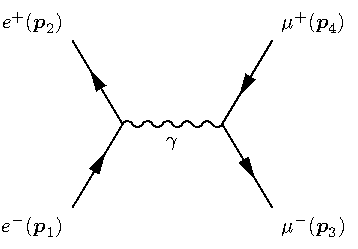
\includegraphics[width=.35\linewidth]{图/eemm.pdf}
%  \begin{fmffile}{eemumu}
%   \fmfframe(20,20)(20,20){\begin{fmfgraph*}(120,80)
%     \fmfleft{i1,i2}
%     \fmfright{o1,o2}
%     \fmflabel{$e^-(\boldsymbol{p}_1)$}{i1}
%     \fmflabel{$e^+(\boldsymbol{p}_2)$}{i2}
%     \fmflabel{$\mu^-(\boldsymbol{p}_3)$}{o1}
%     \fmflabel{$\mu^+(\boldsymbol{p}_4)$}{o2}
%     \fmf{fermion}{i1,v1}
%     \fmf{fermion}{v1,i2}
%     \fmf{fermion}{o2,v2}
%     \fmf{fermion}{v2,o1}
%     \fmf{boson,label=\(\gamma\)}{v1,v2}
%   \end{fmfgraph*}}
% \end{fmffile}
\end{center}
那么根据图中的动量以及费曼规则，我们可以得出其散射振幅：
\begin{equation}
-i\mathcal{M}=\bar{v}({p}_2)(-ie\gamma^\mu)u({p}_1)\frac{-i\eta_{\mu\nu}}{(p_1+p_2)^2}\bar{u}({p}_3)(-ie\gamma^\nu)v({p}_4)
\end{equation}
则我们可易得振幅的模方为：
% \begin{small}
	\begin{equation}
|\mathcal{M}|^2=\frac{e^4\eta_{\mu\nu}\eta_{\lambda\rho}}{(p_1+p_2)^4}\Big(\bar{u}(p_1)\gamma^\rho v(p_2)\Big)\Big(\bar{v}(p_2)\gamma^\mu u(p_1)\Big)\Big(\bar{u}(p_3)\gamma^\nu v(p_4)\Big)\Big(\bar{v}(p_4)\gamma^\lambda u(p_3)\Big)
\end{equation}
% \end{small}
那么当我们进一步计算散射过程可观测量时，则需要考虑极化的因素。对于非极化的散射过程，初态即为非极化粒子束，那么我们则需要对初态粒子的自旋求平均值。而对于末态，则粒子的可以为任意的极化状态，那么我们则要考虑所有可能的末态自旋，即对末态自旋求和。

对于非极化的初态电子，每个电子有2个自旋态，那么自旋态求平均则有一个$\frac{1}{4}$的因子。而对于费米子的自旋求和，则为对其螺旋度求和，即$\gamma^\mu$矩阵4分量求迹。那么最终我们对电子和$\mu$子分别进行自旋求和，然后再乘上初态平均的因子，且利用\eqref{eq:helsum}式的结果，我们可得：
\begin{equation}
\frac{1}{4}\sum_{\text{spin}}|\mathcal{M}|^2=\frac{e^4\eta_{\mu\nu}\eta_{\lambda\rho}}{4(p_1+p_2)^4}\mathrm{tr}\Big[(\slashed{p}_1+m_e)\gamma^\rho(\slashed{p}_2-m_e)\gamma^\mu\Big]\mathrm{tr}\Big[(\slashed{p}_3+m_\mu)\gamma^\nu(\slashed{p}_4-m_\mu)\gamma^\lambda\Big]
\end{equation}
由附录中\eqref{eq:gmtr}式，我们可得：
% \begin{small}
\begin{equation}
\overline{|\mathcal{M}|}^2=8e^4\frac{(p_1\cdot p_4)(p_2\cdot p_3)+(p_1\cdot p_3)(p_2\cdot p_4)+m_e^2(p_3\cdot p_4)+m_\mu^2(p_1\cdot p_2)+2m_e^2 m_\mu^2}{(p_1+p_2)^4}
\end{equation}
% \end{small}
利用四动量守恒及在壳条件，且由\eqref{eq:madsum}式，可将振幅模方化简为：
\begin{equation}
\begin{split}
\overline{|\mathcal{M}|}^2&=8e^4\frac{(p_1\cdot p_4)^2+(p_1\cdot p_3)^2+(m_e^2+m_\mu^2)(m_e^2+p_1\cdot p_2)}{(2p_1\cdot p_2+2m_e^2)^2}\\
&=8e^4\frac{(p_1\cdot p_3)^2+(\frac{s}{2}-p_1\cdot p_3)^2+\frac{s}{2}(m_e^2+m_\mu^2)}{s^2}
\end{split}
\end{equation}
%在通常的高能物理能区，电子的质量极其地微小

对于高能标下的该散射过程，由于电子质量和$\mu$子质量都非常小，所以可以忽略不记\(m_e\approx m_\mu\approx0\)。并且将所有四动量内积项转换为用Mandelstam表示的形式
%\footnote{粒子质量可忽略，且可考虑在质心系\[\begin{split}s&\approx2p_1\cdot p_2\approx2p_3\cdot p_4\\t&\approx-2p_1\cdot p_3\approx -2p_2\cdot p_4\\u&\approx-2p_1\cdot p_4\approx -2p_2\cdot p_3	\end{split}\]}
，那么结果可以写为：
\begin{equation}
\overline{|\mathcal{M}|}^2\approx2e^4\frac{u^2+t^2}{s^2}=2e^4\left(1+2\frac{t}{s}+2\frac{t^2}{s^2}\right)
\end{equation}
由于这一类过程的振幅模方反比于$s^2$，我们通常称之为$s$反应道。

此时我们已经可以计算具体的可观测量，即散射截面。由\eqref{eq:difxsec}式，我们可得二体散射的微分截面：
\begin{equation}
\begin{split}
\frac{\mathrm{d}\sigma}{\mathrm{d}\Omega}=\frac{\overline{|\mathcal{M}|}^2}{64\pi^2 s}\sqrt{\frac{1-\frac{4m_\mu^2}{s}}{1-\frac{4m_e^2}{s}}}
\end{split}
\end{equation}
其中$\alpha=\frac{e^2}{4\pi}$为精细结构常数。代入振幅模方可得：
\begin{equation}
\begin{split}
\frac{\mathrm{d}\sigma}{\mathrm{d}\Omega}&=\frac{\alpha^2}{2s}\left(1+2\frac{t}{s}+2\frac{t^2}{s^2}-4(m_e^2+m_\mu^2)(1+\frac{t}{s})+2(m_e^2+m_\mu^2)^2\right)\sqrt{\frac{s-{4m_\mu^2}}{s-{4m_e^2}}}\\&\approx\frac{\alpha^2}{2s}\left(1+2\frac{t}{s}+2\frac{t^2}{s^2}\right)
\end{split}
\end{equation}

考虑选取质心系作为我们的参考系，那么$\boldsymbol{p}_1$和$\boldsymbol{p}_2$等大反向，而$\boldsymbol{p}_1$和$\boldsymbol{p}_3$之间的夹角则为横向的散射角$\theta$。由于Mandelstam变量具有洛伦兹不变性，因此这三个变量在我们选取特定参考系时都不会发生改变。此时我们可计算出：
\begin{equation}
p_1\cdot p_3=\frac{s}{4}\left(1-\sqrt{(1-\frac{4m_\mu^2}{s})(1-\frac{4m_e^2}{s})}\cos\theta\right)=\frac{m_e^2+m_\mu^2-t}{2}
\end{equation}
而在极端相对论情形质心系中，则有Mandelstam变量和横向散射角$\theta$的关系：
\begin{equation}
t\approx-\frac{s}{2}(1-\cos\theta),\qquad u\approx-\frac{s}{2}(1+\cos\theta)
\end{equation}
微分截面则可表示为径向角$\theta$的函数：
\begin{equation}
\begin{split}
\frac{\mathrm{d}\sigma}{\mathrm{d}\Omega}(\theta)&=\frac{\alpha^2}{4s}\left(1+(1-\frac{4m_\mu^2}{s})(1-\frac{4m_e^2}{s})\cos^2\theta+\frac{4(m_e^2+m_\mu^2)}{s}\right)\sqrt{\frac{s-4m_\mu^2}{s-4m_e^2}}\\
&\approx\frac{\alpha^2}{4s}(1+\cos^2\theta)
\end{split}
\end{equation}
那么对立体角进行积分，我们则可得该过程的总散射截面为：
\begin{equation}
\sigma=\frac{4\pi\alpha^2}{3s}\left(1+\frac{2}{s}(m_e^2+m_\mu^2)+\frac{4}{s^2}m_e^2 m_\mu^2\right)\sqrt{\frac{s-4m_\mu^2}{s-4m_e^2}}\approx\frac{4\pi\alpha^2}{3 s}
\end{equation}

\begin{itemize}
\item 另外考虑电子和$\mu$子的外围散射过程：
\end{itemize}
\begin{equation}
e^- +\mu^-\longrightarrow e^-+\mu^-
\end{equation}
该过程的树图级别费曼图为：
% \newline
\begin{figure}[h]
\centering
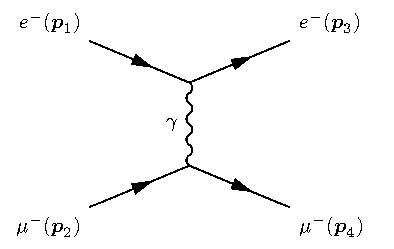
\includegraphics[width=0.33\textwidth]{图/emem.pdf}
% \begin{fmffile}{emu_emu}
%   \begin{fmfgraph*}(120,80)
%     \fmfleft{i1,i2}
%     \fmfright{o1,o2}
%     \fmflabel{$\mu^-(\boldsymbol{p}_2)$}{i1}
%     \fmflabel{$e^-(\boldsymbol{p}_1)$}{i2}
%     \fmflabel{$\mu^-(\boldsymbol{p}_3)$}{o1}
%     \fmflabel{$e^-(\boldsymbol{p}_4)$}{o2}
%     \fmf{fermion}{i1,v1,o1}
%     \fmf{fermion}{i2,v2,o2}
%     \fmf{photon,label=$\gamma$}{v1,v2}
%   \end{fmfgraph*}
% \end{fmffile}
\caption{}
\end{figure}
% \newline
则我们可得散射振幅为：
\begin{equation}
-i\mathcal{M}=\bar{u}({p}_3)(-ie\gamma^\mu)u({p}_1)\frac{-i\eta_{\mu\nu}}{(p_1-p_3)^2}\bar{u}({p}_4)(-ie\gamma^\nu)u({p}_2)
\end{equation}
则同理，并且我们考虑高能情形下的极端相对论极限，我们可计算的振幅模方为：
\begin{equation}
\overline{|\mathcal{M}|}^2\approx8e^4\frac{(p_1\cdot p_2)(p_3\cdot p_4)+(p_1\cdot p_4)(p_2\cdot p_3)}{(p_1-p_3)^2}\approx2e^4\frac{s^2+u^2}{t^2}
\end{equation}
我们通常将这种过程称为$t$反应道。

我们可得微分截面：
\begin{equation}
\frac{\mathrm{d}\sigma}{\mathrm{d}\Omega}(\theta)\approx\frac{\alpha^2}{2s}\frac{4+(1+\cos\theta)^2}{(1-\cos\theta)^2}
\end{equation}
我们可看到，这样的过程在$0\textdegree$角处极大地增幅。

\subparagraph{Bhabha散射}即为正负电子之间发生对撞，之后仍然产生一对正负电子的过程：
\begin{equation}
e^-+e^+\longrightarrow\; e^-+e^+
\end{equation}
对于这样的一个相互作用过程，我们可以用两个不同的费曼图来描述，分别对应$s$反应道和$t$反应道。由量子力学的相干叠加原理，实际的过程则是这两个反应道相干叠加的结果。
\begin{figure}[h]
\centering
	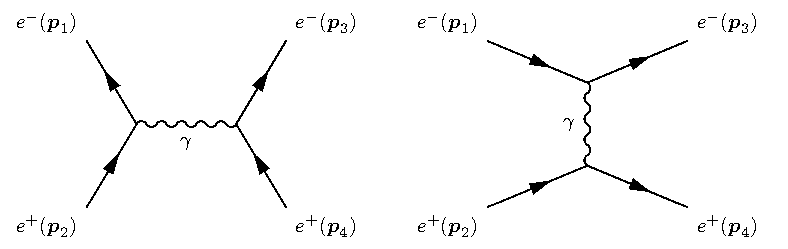
\includegraphics[width=.75\textwidth]{图/bhabha.pdf}
 % \vspace{20pt}
%  \begin{fmffile}{bhabha_s}
%   \begin{fmfgraph*}(120,80)
%     \fmfleft{i1,i2}
%     \fmfright{o1,o2}
%     \fmflabel{$e^-(\boldsymbol{p}_2)$}{i1}
%     \fmflabel{$e^-(\boldsymbol{p}_1)$}{i2}
%     \fmflabel{$e^-(\boldsymbol{p}_4)$}{o1}
%     \fmflabel{$e^-(\boldsymbol{p}_3)$}{o2}
%     \fmf{fermion}{i1,v1,i2}
%     \fmf{fermion}{o1,v2,o2}
%     \fmf{photon,label=$\gamma$}{v1,v2}
%   \end{fmfgraph*}
% \end{fmffile} \qquad\qquad \begin{fmffile}{bhabha_t}
%   \begin{fmfgraph*}(120,80)
%     \fmfleft{i1,i2}
%     \fmfright{o1,o2}
%     \fmflabel{$e^-(\boldsymbol{p}_2)$}{i1}
%     \fmflabel{$e^-(\boldsymbol{p}_1)$}{i2}
%     \fmflabel{$e^-(\boldsymbol{p}_4)$}{o1}
%     \fmflabel{$e^-(\boldsymbol{p}_3)$}{o2}
%     \fmf{fermion}{i1,v1,o1}
%     \fmf{fermion}{i2,v2,o2}
%     \fmf{photon,label=$\gamma$}{v1,v2}
%   \end{fmfgraph*}
% \end{fmffile}
 % \vspace{20pt}
 \caption{}
\end{figure}
根据费曼图我们可以得到具体的散射振幅，而总的散射振幅则为这两张费曼图对应的散射振幅之和：
\begin{equation}
\begin{split}
-i\mathcal{M}=&\bar{v}({p}_2)(-ie\gamma^\mu)u({p}_1)\frac{-i\eta_{\mu\nu}}{(p_1+p_2)^2}\bar{u}({p}_3)(-ie\gamma^\nu)v({p}_4)\\&+\bar{u}({p}_3)(-ie\gamma^\mu)u({p}_1)\frac{-i\eta_{\mu\nu}}{(p_1-p_3)^2}\bar{v}({p}_2)(ie\gamma^\nu)v({p}_4)
\end{split}
\end{equation}
那么振幅模方则是该散射振幅之和的模方，同样考虑极端相对论情形：
\begin{equation}
\overline{|\mathcal{M}|}^2=2e^4\left(\frac{u^2+t^2}{s^2}+\frac{s^2+u^2}{t^2}+\frac{2u^2}{s\cdot t}\right)
\end{equation}
微分截面为：
\begin{equation}
\frac{\mathrm{d}\sigma}{\mathrm{d}\Omega}(\theta)=\frac{\alpha^2}{2s}\left(\frac{1+\cos^2\theta}{2}+\frac{4+\cos\theta(1+\cos\theta)^2}{(1-\cos\theta)^2}\right)
\end{equation}


\subparagraph{M\o{}ller散射}即为电子和电子之间的散射：
\begin{equation}
e^-+e^-\longrightarrow\; e^-+e^-
\end{equation}
\begin{figure}[h]
\centering
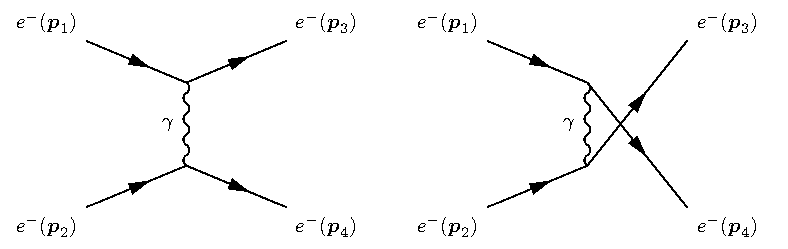
\includegraphics[width=0.75\textwidth]{图/moeller.pdf}
%  \vspace{20pt}
%  \begin{fmffile}{moeller_t}
%   \begin{fmfgraph*}(120,80)
%     \fmfleft{i1,i2}
%     \fmfright{o1,o2}
%     \fmflabel{$e^-(\boldsymbol{p}_2)$}{i1}
%     \fmflabel{$e^-(\boldsymbol{p}_1)$}{i2}
%     \fmflabel{$e^-(\boldsymbol{p}_4)$}{o1}
%     \fmflabel{$e^-(\boldsymbol{p}_3)$}{o2}
%     \fmf{fermion}{i1,v1,o1}
%     \fmf{fermion}{i2,v2,o2}
%     \fmf{photon,label=$\gamma$}{v1,v2}
%   \end{fmfgraph*}
% \end{fmffile} \qquad\qquad\qquad\begin{fmffile}{moeller_u}
%   \begin{fmfgraph*}(120,80)
%     \fmfleft{i1,i2}
%     \fmfright{o1,o2}
%     \fmflabel{$e^-(\boldsymbol{p}_2)$}{i1}
%     \fmflabel{$e^-(\boldsymbol{p}_1)$}{i2}
%     \fmflabel{$e^-(\boldsymbol{p}_4)$}{o1}
%     \fmflabel{$e^-(\boldsymbol{p}_3)$}{o2}
%     \fmf{fermion}{i1,v1}
%     \fmf{fermion}{i2,v2}
%     \fmf{phantom}{v1,o1}
%     \fmf{phantom}{v2,o2}
%     \fmf{fermion,tension=0}{v1,o2}
%     \fmf{fermion,tension=0}{v2,o1}
%     \fmf{photon,label=$\gamma$}{v1,v2}
%   \end{fmfgraph*}
% \end{fmffile}
%  \vspace{20pt}
\caption{}
\end{figure}
我们知道，如果$t$反应道的末态粒子为全同粒子，那么这两粒子则具有交换对称性不可分辨。因此则会有右图费曼图，即产生一个额外的反应道。这一个额外的反应道我们称之为$u$反应道。

对于这个散射过程，我们可以得到其散射振幅：
\begin{equation}
\begin{split}
-i\mathcal{M}=&\bar{u}({p}_3)(-ie\gamma^\mu)u({p}_1)\frac{-i\eta_{\mu\nu}}{(p_1-p_3)^2}\bar{u}({p}_4)(-ie\gamma^\nu)u({p}_2)\\
&+\bar{u}({p}_4)(-ie\gamma^\mu)u({p}_1)\frac{-i\eta_{\mu\nu}}{(p_1-p_4)^2}\bar{u}({p}_3)(-ie\gamma^\nu)u({p}_2)
\end{split}
\end{equation}

在极端相对论情形下，振幅模方为：
\begin{equation}
\overline{|\mathcal{M}|}^2=2e^4\left(\frac{s^2+u^2}{t^2}+\frac{s^2+t^2}{u^2}+\frac{2s^2}{t\cdot u}\right)
\end{equation}
微分截面为：
\begin{equation}
\frac{\mathrm{d}\sigma}{\mathrm{d}\Omega}(\theta)=\frac{\alpha^2}{2s}\left(\frac{4+(1+\cos\theta)^2}{(1-\cos\theta)^2}+\frac{4+(1-\cos\theta)^2}{(1+\cos\theta)^2}+\frac{1}{2(1-\cos^2\theta)}\right)
\end{equation}

\subparagraph{Compton散射} 即为光子与电子发生的散射。由于Compton散射发生在较高能区下，因此不同于电子光子的汤姆逊散射（弹性散射），此过程为非弹性散射。所以经典的电动力学并不能精确计算Compton散射，而需要用到量子电动力学进行计算。
\begin{equation}
e^-+\gamma\rightarrow e^-+\gamma
\end{equation}
\begin{figure}[h]
\centering
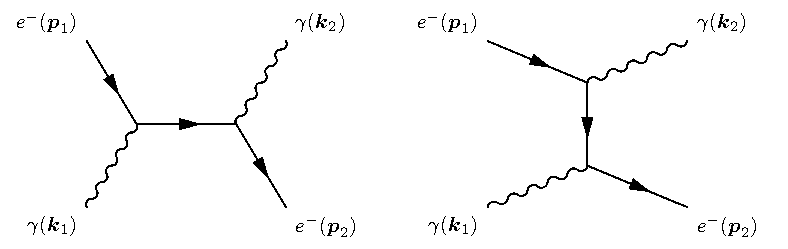
\includegraphics[width=.75\textwidth]{图/compton.pdf}
% \vspace{20pt}
%  \begin{fmffile}{compton_s}
%   \begin{fmfgraph*}(120,80)
%     \fmfleft{i1,i2}
%     \fmfright{o1,o2}
%     \fmflabel{$\gamma(\boldsymbol{k}_1)$}{i1}
%     \fmflabel{$e^-(\boldsymbol{p}_1)$}{i2}
%     \fmflabel{$e^-(\boldsymbol{p}_2)$}{o1}
%     \fmflabel{$\gamma(\boldsymbol{k}_2)$}{o2}
%     \fmf{boson}{i1,v1}
%     \fmf{fermion}{i2,v1}
%     \fmf{boson}{v2,o2}
%     \fmf{fermion}{v2,o1}
%     \fmf{fermion}{v1,v2}
%   \end{fmfgraph*}
% \end{fmffile} \qquad\qquad\qquad \begin{fmffile}{compton_t}
%   \begin{fmfgraph*}(120,80)
%     \fmfleft{i1,i2}
%     \fmfright{o1,o2}
%     \fmflabel{$\gamma(\boldsymbol{k}_1)$}{i1}
%     \fmflabel{$e^-(\boldsymbol{p}_1)$}{i2}
%     \fmflabel{$e^-(\boldsymbol{p}_2)$}{o1}
%     \fmflabel{$\gamma(\boldsymbol{k}_2)$}{o2}
%     \fmf{boson}{i1,v1}
%     \fmf{fermion}{v1,o1}
%     \fmf{fermion}{i2,v2}
%     \fmf{boson}{v2,o2}
%     \fmf{fermion}{v2,v1}
%   \end{fmfgraph*}
% \end{fmffile}
% \vspace{20pt}
\caption{}
\end{figure}
由费曼规则，我们可得：
\begin{equation}
\begin{split}
-i\mathcal{M}=&\bar{u}({p}_2)(-ie)\slashed{\varepsilon}^*({k}_2)\frac{i(\slashed{p}_1+\slashed{k}_1+m)}{(p_1+k_1)^2-m^2}\slashed{\varepsilon}({k}_1)(-ie)u({p}_1)\\&+\bar{u}({p}_2)(-ie)\slashed{\varepsilon}({k}_1)\frac{i(\slashed{p}_1-\slashed{k}_2+m)}{(p_1-k_2)^2-m^2}\slashed{\varepsilon}^*({k}_2)(-ie)u({p}_1)\\
&\hspace{-1.2cm}=-ie^2\bar{u}(p_2)\left[\frac{\slashed{\varepsilon}^*(k_2)(\slashed{p}_1+\slashed{k}_1+m)\slashed{\varepsilon}(k_1)}{(p_1+k_1)^2-m^2}+\frac{\slashed{\varepsilon}(k_1)(\slashed{p}_1-\slashed{k}_2+m)\slashed{\varepsilon}^*(k_2)}{(p_1-k_2)^2-m^2}\right]u(p_1)
\end{split}
\end{equation}
其中利用了$\gamma^\mu$矩阵的反对易关系以及各粒子的质量在壳条件。我们知道光子极化矢量必然正交与光子动量，则有$k_1\cdot\varepsilon_1=0,k_2\cdot\varepsilon_2=0$。此时我们还可以利用$u_1$的运动方程$(-\slashed{p}_1+m)u(p_1)=0$，则可得：
\begin{equation}
-i\mathcal{M}=-ie^2\bar{u}_2\Big(\frac{\slashed{\varepsilon}^*_2\slashed{k}_1\slashed{\varepsilon}_1+2\slashed{\varepsilon}^*_2p_1\cdot\varepsilon_1}{2p_1\cdot k_1}+\frac{\slashed{\varepsilon}_1\slashed{k}_2\slashed{\varepsilon}^*_2-2\slashed{\varepsilon}_1p_1\cdot\varepsilon^*_2}{2p_1\cdot k_2}\Big)u_1
\end{equation}

考虑非极化过程的自旋求和，对于电子而言我们已经在之前进行过讨论，而对于光子而言，我们则引用\eqref{eq:phopolsum}式可得光子极化矢量的求和条件$\sum_{r=1}^3\varepsilon^r_\mu{\varepsilon^*}^r_\nu=-\eta_{\mu\nu}$。且考虑初态粒子求平均，则有：
\begin{equation}
\begin{split}
\overline{|\mathcal{M}|}^2=\frac{e^4}{4}\eta_{\mu\rho}\eta_{\nu\sigma} \mathrm{tr}\Big[&\left(\frac{\gamma^\mu \slashed{k}_1\gamma^\nu+2\gamma^\mu p_1^\nu}{2p_1\cdot k_1}+\frac{\gamma^\nu \slashed{k}_2\gamma^\mu-2\gamma^\nu p_1^\mu}{2p_1\cdot k_2}\right)(\slashed{p}_1+m)\\
&\left(\frac{\gamma^\sigma \slashed{k}_1\gamma^\rho+2\gamma^\rho p_1^\sigma}{2p_1\cdot k_1}+\frac{\gamma^\rho \slashed{k}_2\gamma^\sigma-2\gamma^\sigma p_1^\rho}{2p_1\cdot k_2}\right)(\slashed{p}_2+m)\Big]
\end{split}
\end{equation}
我们利用四动量守恒可得如下关系：
\begin{align}
&p_2\cdot k_2=p_1\cdot k_1, &p_2\cdot k_1=p_1\cdot k_2 &\notag\\
&p_1\cdot p_2=m^2+p_1\cdot k_1-p_1\cdot k_2, &k_1\cdot k_2=p_1\cdot k_1&-p_1\cdot k_2
\end{align}
然后进行求迹并化简可得：
% \begin{small}
\begin{equation}
\overline{|\mathcal{M}|}^2=2e^4\left[\frac{p_1\cdot k_2}{p_1\cdot k_1}+\frac{p_1\cdot k_1}{p_1\cdot k_2}+2m^2\left(\frac{1}{p_1\cdot k_1}-\frac{1}{p_1\cdot k_2}\right)+m^4\left(\frac{1}{p_1\cdot k_1}-\frac{1}{p_1\cdot k_2}\right)^2\right]
\end{equation}
% \end{small}

对于Compton散射，我们通常考虑的实验室坐标系为初态电子的静止坐标系，即高能光子射击静止的靶电子。那么初态电子的四动量就可以表示为$p^\mu_1=(m,0,0,0)$，因此$p_1\cdot k=m\omega$，$\omega=k^0$为光子动量的类时分量，即光的角频率。而由靶心系中的四动量守恒我们可得Compton散射公式：
\begin{equation}
\omega_2=\frac{\omega_1}{1+\frac{\omega_1}{m}(1-\cos\theta)},\qquad \lambda'=\lambda+\lambda_\text{c}(1-\cos\theta)
\end{equation}
其中$\lambda_\text{c}=\frac{2\pi}{m}$为Compton波长，而$\lambda$为入射光波长，$\theta$则为入射光子与出射光子的夹角$\cos\theta=\frac{\boldsymbol{k}_1\cdot\boldsymbol{k}_2}{|\boldsymbol{k}_1||\boldsymbol{k}_2|}$。

而对于靶心系中的末态相空间，由\eqref{eq:dlips}式可得：
\begin{equation}
\begin{split}
\mathrm{d}Q_\text{LIPS}=&\frac{1}{4(2\pi)^2}\frac{\delta(|\boldsymbol{k}_2|-k_2^0){|\boldsymbol{k}_2|}^2\mathrm{d}|\boldsymbol{k}_2|\mathrm{d}\Omega}{\left|1-\frac{(\boldsymbol{k}_1-\boldsymbol{k}_2)\cdot\boldsymbol{k}_2}{p_2^0|\boldsymbol{k}_2|}\right|_{\boldsymbol{k}_2=k_2^0}\;k_2^0 p_2^0}=\frac{{k_2^0}^2\mathrm{d}\Omega}{4(2\pi)^2 \frac{p_2\cdot k_2}{k_2^0 p_2^0} k_2^0 p_2^0}\\
=&\frac{{k_2^0}^2\mathrm{d}\Omega}{16\pi^2mk_1^0}
\end{split}
\end{equation}
加上散射初态粒子的部分，我们可得微分截面为：
\begin{equation}
\frac{\mathrm{d}\sigma}{\mathrm{d}\Omega}=\frac{\overline{|\mathcal{M}|}^2{k_2^0}^2}{64\pi^2(p_1\cdot k_1)mk_1^0}
\end{equation}

利用Compton散射公式，并将振幅模方代入到微分截面中，我们可得：
\begin{equation}
\frac{\mathrm{d}\sigma}{\mathrm{d}\Omega}=\frac{\alpha^2}{2m^2}\left(\frac{\omega_2}{\omega_1}\right)^2\left(\frac{\omega_2}{\omega_1}+\frac{\omega_1}{\omega_2}-\sin^2\theta\right)
\end{equation}
上式即为光子的Compton散射微分截面，称为Klein-仁科公式。

我们知道电子经典半径为$r_e=\frac{\alpha}{m}$。则微分截面可写为仅关于入射光波长$\lambda$和散射角$\theta$的形式：
\begin{equation}
\frac{\mathrm{d}\sigma}{\mathrm{d}\Omega}=\frac{r_e^2}{2}\left[\frac{1+\cos^2\theta}{\left(1+\frac{\lambda_\text{c}}{\lambda}(1-\cos\theta)\right)^2}+\frac{\left(\frac{\lambda_\text{c}}{\lambda}(1-\cos\theta)\right)^2}{\left(1+\frac{\lambda_\text{c}}{\lambda}(1-\cos\theta)\right)^3}\right]
\end{equation}
那么对散射立体角积分即可得总的Compton散射截面：
\begin{equation}
\begin{split}
\sigma=&\pi r_e^2\left[\frac{4}{\left(\frac{\lambda_\text{c}}{\lambda}\right)^2}+\frac{2(1+\frac{\lambda_\text{c}}{\lambda})}{\left(1+2\frac{\lambda_\text{c}}{\lambda}\right)^2}-\frac{2+(2-\frac{\lambda_\text{c}}{\lambda})\frac{\lambda_\text{c}}{\lambda}}{\left(\frac{\lambda_\text{c}}{\lambda}\right)^3}\ln\left(1+2\frac{\lambda_\text{c}}{\lambda}\right)\right]
\end{split}
\end{equation}
如果当入射波波长相较于Compton波长极大时，$\frac{\lambda_\text{c}}{\lambda}\rightarrow0$，总截面则近似为：
\begin{equation}
\begin{split}
\sigma&\approx\pi r_e^2\left[\frac{8}{3}-\frac{16}{3}\frac{\lambda_\text{c}}{\lambda}+\frac{208}{15}\left(\frac{\lambda_\text{c}}{\lambda}\right)^2+\cdots\right]\\
&\approx\frac{8}{3}\pi r_e^2
\end{split}
\end{equation}
即在长波极限下，则Compton散射截面回归到经典的汤姆逊散射截面，符合量子力学的经典极限。

\subparagraph{正负电子对生成}
我们知道只要当两束光子的能量大于2个电子质量的时候，就可以相互作用从真空中产生一对正负电子对。该过程即为：
\[\gamma+\gamma\rightarrow e^+ + e^-\]
\begin{figure}[h]
\centering
	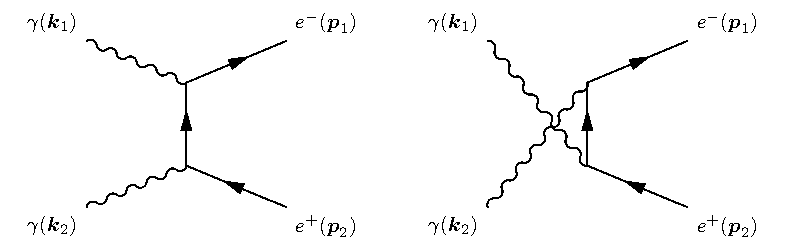
\includegraphics[width=.75\textwidth]{图/pair.pdf}
%  \vspace{20pt}
%  \begin{fmffile}{pair_t}
%   \begin{fmfgraph*}(120,80)
%     \fmfleft{i1,i2}
%     \fmfright{o1,o2}
%     \fmflabel{$\gamma(\boldsymbol{k}_2)$}{i1}
%     \fmflabel{$\gamma(\boldsymbol{k}_1)$}{i2}
%     \fmflabel{$e^+(\boldsymbol{p}_2)$}{o1}
%     \fmflabel{$e^-(\boldsymbol{p}_1)$}{o2}
%     \fmf{boson}{i1,v1}
%     \fmf{fermion}{o1,v1}
%     \fmf{boson}{i2,v2}
%     \fmf{fermion}{v2,o2}
%     \fmf{fermion}{v1,v2}
%   \end{fmfgraph*}
% \end{fmffile} \qquad\qquad\qquad\begin{fmffile}{pair_u}
%   \begin{fmfgraph*}(120,80)
%     \fmfleft{i1,i2}
%     \fmfright{o1,o2}
%     \fmflabel{$\gamma(\boldsymbol{k}_2)$}{i1}
%     \fmflabel{$\gamma(\boldsymbol{k}_1)$}{i2}
%     \fmflabel{$e^+(\boldsymbol{p}_2)$}{o1}
%     \fmflabel{$e^-(\boldsymbol{p}_1)$}{o2}
%     \fmf{boson,tension=0}{i1,v2}
%     \fmf{boson,tension=0}{i2,v1}
%     \fmf{phantom}{v1,i1}
%     \fmf{phantom}{v2,i2}
%     \fmf{fermion}{o1,v1}
%     \fmf{fermion}{v2,o2}
%     \fmf{fermion}{v1,v2}
%   \end{fmfgraph*}
% \end{fmffile}
% \vspace{20pt}
 \caption{}
\end{figure}
那么其散射振幅即为：
\begin{equation}
\begin{split}
-i\mathcal{M}=\bar{u}(p_1)(-ie)\slashed{\varepsilon}(k_1)\frac{i(\slashed{k}_1-\slashed{p}_1+m)}{(k_1-p_1)^2-m^2}\slashed{\varepsilon}(k_2)(-ie)v(p_2)\\
+\bar{u}(p_1)(-ie)\slashed{\varepsilon}(k_2)\frac{i(\slashed{k}_2-\slashed{p}_1+m)}{(k_2-p_1)^2-m^2}\slashed{\varepsilon}(k_1)(-ie)v(p_2)\\
=-ie^2\bar{u}_1\left(\frac{2\varepsilon_1\cdot p_1-\slashed{\varepsilon}_1\slashed{k}_1}{2k_1\cdot p_1}\slashed{\varepsilon}_2+\frac{2\varepsilon_2\cdot p_1-\slashed{\varepsilon}_2\slashed{k}_2}{2k_2\cdot p_1}\slashed{\varepsilon}_1\right)v_2
\end{split}
\end{equation}
与Compton散射的计算过程同理，我们可得非极化的振幅模方：
% \begin{small}
\begin{equation}
\overline{|\mathcal{M}|}^2=2e^2\left[\frac{p_1\cdot k_2}{p_1\cdot k_1}+\frac{p_1\cdot k_1}{p_1\cdot k_2}+2m^2\left(\frac{1}{p_1\cdot k_1}+\frac{1}{p_1\cdot k_2}\right)-m^4\left(\frac{1}{p_1\cdot k_1}+\frac{1}{p_1\cdot k_2}\right)^2\right]
\end{equation}
% \end{small}
可以看出，该振幅模方实际等同于将Compton散射振幅模方中的动量替换为$p_1\rightarrow-p_1$和$k_2\rightarrow-k_2$，且对$m^4$项加额外的负号。

对于该过程，我们则可选取质心系，那么我们可得动量的内积：
\begin{equation}
p_1\cdot k_1=m^2\frac{1-\beta\cos\theta}{1-\beta^2},\qquad p_1\cdot k_2=m^2\frac{1+\beta\cos\theta}{1-\beta^2}
\end{equation}
$\theta$角即为动量中心系的横向散射角，而$\beta=v$则为出射电子的相对论速度。由于选取的是质心系，因此两电子的速度相等，都可以用$\beta$来描述。由此我们可得末态相空间为：
\begin{equation}
\mathrm{d}Q_\text{LIPS}=\frac{\beta}{32\pi^2}\mathrm{d}\Omega
\end{equation}
因此微分截面可表为：
\begin{equation}
\frac{\mathrm{d}\sigma}{\mathrm{d}\Omega}=\frac{\overline{|\mathcal{M}|}^2(1-\beta^2)\beta}{256\pi^2m^2}
\end{equation}
代入振幅模方，可得正负电子对生成过程的微分截面：
\begin{equation}
\frac{\mathrm{d}\sigma}{\mathrm{d}\Omega}=\frac{\alpha^2(1-\beta^2)\beta}{4m^2}\left(\frac{1+\beta^2\cos^2\theta+2(1-\beta^2)}{1-\beta^2\cos^2\theta}-\frac{2(1-\beta^2)^2}{(1-\beta^2\cos^2\theta)^2}\right)
\end{equation}
对其积分，则可得正负电子对生成过程的总散射截面：
\begin{equation}
\sigma=\frac{\pi r_e^2}{2}(1-\beta^2)\left(2\beta(\beta^2-2)-(\beta^4-3)\ln\Big(\frac{1+\beta}{1-\beta}\Big)\right)
\end{equation}

\subparagraph{正负电子对湮灭} 而当一对正负电子对相遇时，则会相互湮灭，并将能量转化为光子。该过程即为：
\[e^+ + e^-\rightarrow \gamma+\gamma\]
\begin{figure}[h]
\centering
	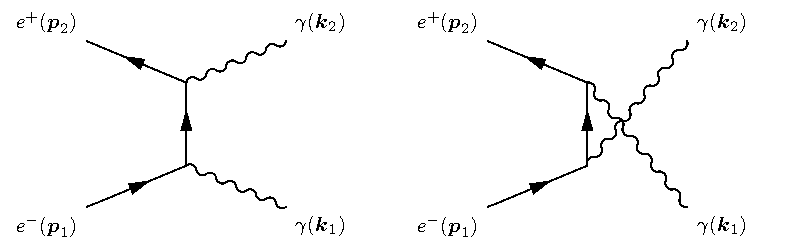
\includegraphics[width=.75\textwidth]{图/annihilation.pdf}
%  \vspace{20pt}
%  \begin{fmffile}{annihilation_t}
%   \begin{fmfgraph*}(120,80)
%     \fmfleft{i2,i1}
%     \fmfright{o2,o1}
%     \fmflabel{$\gamma(\boldsymbol{k}_1)$}{o1}
%     \fmflabel{$\gamma(\boldsymbol{k}_2)$}{o2}
%     \fmflabel{$e^-(\boldsymbol{p}_1)$}{i1}
%     \fmflabel{$e^+(\boldsymbol{p}_2)$}{i2}
%     \fmf{fermion}{i1,v1}
%     \fmf{boson}{o1,v1}
%     \fmf{fermion}{v2,i2}
%     \fmf{boson}{v2,o2}
%     \fmf{fermion}{v1,v2}
%   \end{fmfgraph*}
% \end{fmffile} \qquad\qquad\qquad\begin{fmffile}{annihilation_u}
%   \begin{fmfgraph*}(120,80)
%     \fmfleft{i2,i1}
%     \fmfright{o2,o1}
%     \fmflabel{$\gamma(\boldsymbol{k}_1)$}{o1}
%     \fmflabel{$\gamma(\boldsymbol{k}_2)$}{o2}
%     \fmflabel{$e^-(\boldsymbol{p}_1)$}{i1}
%     \fmflabel{$e^+(\boldsymbol{p}_2)$}{i2}
%     \fmf{boson,tension=0}{o1,v2}
%     \fmf{boson,tension=0}{o2,v1}
%     \fmf{phantom}{v1,o1}
%     \fmf{phantom}{v2,o2}
%     \fmf{fermion}{i1,v1}
%     \fmf{fermion}{v2,i2}
%     \fmf{fermion}{v1,v2}
%   \end{fmfgraph*}
% \end{fmffile}
% \vspace{20pt}
 \caption{}
\end{figure}
由于该过程实际上为正负电子对生成的逆过程，所以非极化振幅模方与此仅差一负号：
% \begin{small}
	\begin{equation}
	\overline{|\mathcal{M}|}^2=-2e^2\left[\frac{p_1\cdot k_2}{p_1\cdot k_1}+\frac{p_1\cdot k_1}{p_1\cdot k_2}+2m^2\left(\frac{1}{p_1\cdot k_1}+\frac{1}{p_1\cdot k_2}\right)-m^4\left(\frac{1}{p_1\cdot k_1}+\frac{1}{p_1\cdot k_2}\right)^2\right]
	\end{equation}
% \end{small}
同样我们选取质心系作为参考系。然而过程的初末态并不相同，则实际的散射截面关于入射粒子及末态相空间的部分则会不同：
\begin{equation}
\frac{\mathrm{d}\sigma}{\mathrm{d}\Omega}=\frac{\overline{|\mathcal{M}|}^2}{256\pi^2m^2\gamma\sqrt{\gamma^2-1}}
\end{equation}
其中$\gamma=\frac{\omega}{m}$为出射光频率与电子质量之比，也为初态电子的洛伦兹因子。且我们有：
\begin{equation}
p_1\cdot k_1=m^2(\gamma^2-\gamma\sqrt{\gamma^2-1}\cos\theta),\quad p_1\cdot k_2=m^2(\gamma^2+\gamma\sqrt{\gamma^2-1}\cos\theta)
\end{equation}
可得正负电子湮灭的微分截面为：
\begin{equation}
\frac{\mathrm{d}\sigma}{\mathrm{d}\Omega}=\frac{\alpha^2}{4m^2\gamma\sqrt{\gamma^2-1}}\left(\frac{2}{(\gamma^2-(\gamma^2-1)\cos^2\theta)^2}-\frac{\gamma^2+(\gamma^2-1)\cos^2\theta+2}{\gamma^2-(\gamma^2-1)\cos^2\theta}\right)
\end{equation}
那么总的散射截面为：
\begin{equation}
\sigma={\pi r_e^2}\left(\frac{1-2\gamma^2-2\gamma^4}{\gamma^4(\gamma^2-1)}\ln\left(\gamma+\sqrt{\gamma^2-1}\right)+\frac{1+\gamma^2}{\gamma^3\sqrt{\gamma^2-1}}\right)
\end{equation}
%\subsection*{极化散射过程与螺旋度结构}
%\subsubsection{极化费米子}
%\subsubsection{极化光子}


\section{QED辐射修正}
\subsection{QED单圈重整化}
当我们考虑QED的圈图修正时，则需要讨论重整化QED理论。那么我们可以定义裸的QED理论，同时有裸场、裸物理量与重整化场、重整化物理量的关系：
\begin{equation}
\psi_0=\sqrt{Z_\psi}\psi_r,\quad A_0^\mu=\sqrt{Z_A}A^\mu_r,\quad m_0=Z_m m_r,\quad e_0=Z_e e_r
\end{equation}
则重整化QED Lagrangian可以写为：
\begin{equation}
\mathscr{L}_\text{QED}=iZ_\psi\bar{\psi}_r\slashed{\partial}\psi_r- Z_m Z_\psi m_r \bar{\psi}_r\psi_r-\frac{1}{4}Z_A F_{\mu\nu}^r {F^r}^{\mu\nu}-e_r \sqrt{Z_A}Z_\psi Z_e \bar{\psi}_r \slashed{A}_r \psi_r
\end{equation}
此时我们可从此Lagrangian中得到重整化的3点函数和费米子传播子逆：
\begin{equation}
S^{-1}_r(p)=Z_\psi(\slashed{p}-m_0),\qquad\tilde{\Gamma}_r^\mu=\sqrt{Z_A}Z_\psi Z_e \gamma^\mu
\end{equation}
代入\eqref{eq:wardf}式的Ward恒等式中，并与树图层面的等式比较，易得：
\begin{equation}
Z_\psi\sqrt{Z_A}Z_e = Z_\psi,\qquad Z_e=Z_A^{-\frac{1}{2}}
\end{equation}
则重整化QED Lagrangian可改写为：
\begin{equation}
	\mathscr{L}_\text{QED}=iZ_\psi\bar{\psi}_r\slashed{\partial}\psi_r- Z_m Z_\psi m_r \bar{\psi}_r\psi_r-\frac{1}{4}Z_A F_{\mu\nu}^r {F^r}^{\mu\nu}-e_r Z_\psi \bar{\psi}_r \slashed{A}_r \psi_r
\end{equation}
%而光子场和费米子场的质量量纲分别为：
%\begin{equation}
%[A_\mu]=\frac{d}{2}-1,\qquad [\psi]=\frac{d-1}{2}
%\end{equation}
\subparagraph{电子自能}
要想求解重整化QED的$Z_\psi, Z_m$，则需要计算费米子的自能，而其中电子作为几乎只参与电磁相互作用的粒子，其自能基本上源自于纯的QED贡献，因此我们则考虑以电子为例费米子的QED重整化。考虑电子的2点格林函数，在单圈层面有如下费曼图，即为电子的自能项：
\begin{figure}[h]
\centering
% \begin{fmffile}{self_electron}
%     \begin{fmfgraph*}(120,100)
%        \fmfleft{i}
%        \fmfright{o}
%        \fmf{fermion,tension=1,label=$p$}{i,v1} 
%        \fmf{fermion,tension=1,label=$p$}{v2,o}
%        \fmf{boson,left,tension=0,label=${k}$}{v1,v2
%        }
%        \fmf{fermion,label=${k-p}$}{v1,v2
%        }
%     \end{fmfgraph*}
% \end{fmffile}
    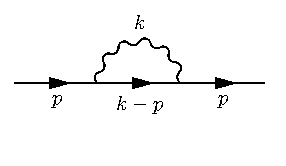
\includegraphics[scale=1.3]{图/self_electron.pdf}
\caption{}
\end{figure}
那么其单圈积分即为：
\begin{equation}
i\Sigma(p)=-e_0^2\int\frac{\mathrm{d}^dk}{(2\pi)^d}\frac{\gamma^\mu(\slashed{p}-\slashed{k}+m)\gamma^\nu}{(p-k)^2-m^2}\frac{(\eta_{\mu\nu}-(1-\xi)\frac{k_\mu k_\nu}{k^2})}{k^2}
\end{equation}
由费米子场量纲$[\psi]=\frac{d-1}{2}$及光子场量纲$[\phi]=\frac{d}{2}-1$可以推算得元电荷的量纲为$[e]=2-\frac{d}{2}$。当我们考虑$d$回归到4维时，我们可以将元电荷用能标参数化为$e_0=e\mu^{\frac{\epsilon}{2}}$。同时为了方便引用费曼积分公式，我们重新定义动量$k_\mu$的方向$k_\mu\rightarrow -k_\mu$，得：
% {\footnotesize 
\begin{equation}
	\begin{split}
i\Sigma(p)&=-e^2\mu^\epsilon\int\frac{\mathrm{d}^dk}{(2\pi)^d}\Big[\frac{\gamma^\mu(\slashed{p}+\slashed{k}+m)\gamma_\mu}{[(p+k)^2-m^2]k^2}-(1-\xi)\frac{\slashed{k}(\slashed{p}+\slashed{k}+m)\slashed{k}}{[(p+k)^2-m^2]k^4}\Big]\\
&=e^2\mu^\epsilon\int\frac{\mathrm{d}^dk}{(2\pi)^d}\Big[\frac{(d-\xi-1)\slashed{k}+(d+\xi-3)\slashed{p}+(1-d-\xi)m}{(k^2+2k\cdot p -m^2+p^2)k^2}+\frac{(1-\xi)2p\cdot k \slashed{k}}{(k^2+2k\cdot p -m^2+p^2)k^4}\Big]
	\end{split}
\end{equation}%}
由费曼积分公式\eqref{eq:loopint}式及其结果\eqref{eq:feyint}式可得：
\begin{equation}
i\Sigma(p)=e^2\mu^\epsilon \Big[I_{1,1}((d+\xi-3)\slashed{p}+(1-d-\xi)m)+(d-\xi-1)\gamma_\mu I^\mu_{1,1}+2(1-\xi)p_\mu\gamma_\nu I^{\mu\nu}_{1,2}\Big]
\end{equation}
进一步化简，可得电子自能：
%\begin{multline}
%\Sigma(p)=\frac{e^2}{16\pi^2}\Big[((1+\xi-\epsilon)\slashed{p}+(\epsilon-3-\xi)m)\Gamma(\frac{\epsilon}{2})\int_0^1\mathrm{d}x\left(\frac{4\pi\mu^2}{\Omega(x)}\right)^{\frac{\epsilon}{2}}\\-(3-\epsilon-\xi)\slashed{p}\Gamma(\frac{\epsilon}{2})\int_0^1\mathrm{d}x\,x\left(\frac{4\pi\mu^2}{\Omega(x)}\right)^{\frac{\epsilon}{2}}\\-(1-\xi)(2p^2 \slashed{p}\int_0^1\mathrm{d}x\frac{x^3}{\Omega}+{\slashed{p}}\Gamma(\frac{\epsilon}{2})\int_0^1\mathrm{d}x\,x\Big(\frac{4\pi\mu^2}{\Omega}\Big)^{\frac{\epsilon}{2}})\Big]
%\end{multline}
\begin{multline}
\Sigma(p)=\frac{e^2}{8\pi^2}\Big[\frac{(2\xi-1)\slashed{p}-(\xi+3)m}{\epsilon}-\frac{\slashed{p}}{2}+m+\Big((\xi-\frac{1}{2})\slashed{p}-\frac{\xi+3}{2}m\Big)\ln \frac{4\pi}{e^\gamma}\\+\int_0^1\mathrm{d}x\Big([(\xi-2)x+\frac{\xi+1}{2}]\slashed{p}-\frac{\xi+3}{2}m\Big)\ln\frac{\mu^2}{\Omega}-(1-\xi)p^2 \slashed{p}\int_0^1\mathrm{d}x\frac{x^3}{\Omega}\Big]
\end{multline}
其中：\begin{equation}
	\Omega=x[(x-1)p^2+m^2]
\end{equation}
\begin{itemize}
\item 当我们选取费曼规范时，即$\xi=1$，则电子自能为：
\end{itemize}
\begin{equation}
\Sigma(p)=\frac{e^2}{8\pi^2}\Big[\frac{\slashed{p}-4m}{\epsilon}+(\frac{\slashed{p}}{2}-2m)\ln 4\pi e^{-\gamma}+m-\frac{\slashed{p}}{2}+\int_0^1\mathrm{d}x[\slashed{p}(1-x)-2m]\ln\frac{\mu^2}{x[(x-1)p^2+m^2]}\Big]
\end{equation}

\begin{itemize}
	\item 当我们选取朗道规范时，即$\xi=0$，则电子自能为：
\end{itemize}
\begin{multline}
	\Sigma(p)=\frac{e^2}{8\pi^2}\Big[\frac{-\slashed{p}-3m}{\epsilon}-\frac{1}{2}\Big(\slashed{p}+3m\Big)\ln 4\pi e^{-\gamma}+m-\slashed{p}\Big(\frac{(p^2-m^2)^2}{p^4}\ln\frac{m^2}{p^2-m^2}\\-2\frac{m^2}{p^2}+\frac{7}{2}\Big)-\int_0^1\mathrm{d}x\Big([2x-\frac{1}{2}]\slashed{p}+\frac{3}{2}m\Big)\ln\frac{\mu^2}{x[(x-1)p^2+m^2]}\Big]
\end{multline}
当我们已经计算出电子自能时，我们则可以考虑对电子场的重整化。即考虑电子的裸2点格林函数\(G_0(x_1,x_2)\sim\langle0|{\psi_0}\bar{\psi}_0|0\rangle\)，代入重整化的电子场后，可得裸2点格林函数与重整化2点格林函数的关系\({G}_r=\frac{1}{Z_\psi}G_0\)，那么可得：
\begin{equation}
{\tilde{G}}_r=\frac{1}{Z_\psi}\Big[\frac{i}{\slashed{p}-Z_m m_r}+\frac{i}{\slashed{p}-m}i\Sigma(p)\frac{i}{\slashed{p}-m}+\mathcal{O}(e^4)+\cdots\Big]
\end{equation}
代入重整化系数\(Z_\psi=1+\delta_\psi, Z_m=1+\delta_m\)，可得：
\begin{equation}
\begin{split}
{\tilde{G}}_r&=\frac{1}{1+\delta_\psi}\Big[\frac{i}{\slashed{p}-m_r-\delta_m m_r}+\frac{i}{\slashed{p}-m_r}i\Sigma(p)\frac{i}{\slashed{p}-m_r}+\mathcal{O}(e^4)+\cdots\Big]\\
&=\frac{i}{\slashed{p}-m_r}+\frac{i}{\slashed{p}-m_r}i\Big(\Sigma(p)+\delta_\psi(\slashed{p}-m_r)-\delta_m m_r\Big)\frac{i}{\slashed{p}-m_r}+\mathcal{O}(e^4)+\cdots
\end{split}
\end{equation}
我们考虑选取费曼规范，并选择最小差值(MS)重整化方案，将自能中的发散项抵消掉，便可求解得：
\begin{equation}
\delta^\text{MS}_\psi=-\frac{e^2}{8\pi^2\epsilon}=-\frac{\alpha}{2\pi\epsilon},\qquad\delta_m^\text{MS}=-\frac{3e^2}{8\pi^2\epsilon}=-\frac{3\alpha}{2\pi\epsilon}
\label{eq:qedferren}
\end{equation}
则我们最终得到在费曼规范下的首一阶电子场重整化和电子质量重整化结果：
\begin{equation}
\psi_0=\psi_r\left(1-\frac{\alpha}{2\pi\epsilon}\right)^\frac{1}{2},\qquad m_0=m_r\left(1-\frac{3\alpha}{2\pi\epsilon}\right)
\end{equation}

带入回电子传播子中，我们可得：
\begin{equation}
    S(p)=\frac{i}{\slashed{p}-m+\Sigma_r(p)}
\end{equation}
其中的质量修正项$\Sigma_r(p)=\Sigma(p)+\delta_\psi(\slashed{p}-m_r)-\delta_m m_r$为消去了发散项的电子自能。在最小差值(MS)方案下为：
\begin{equation}
    \Sigma^\text{MS}_r(p)=\frac{\alpha}{2\pi}\Big[m-\frac{\slashed{p}}{2}+\int_0^1\mathrm{d}x[\slashed{p}(1-x)-2m]\ln\frac{4\pi\mu^2e^{-\gamma}}{x[(x-1)p^2+m^2]}\Big]
\end{equation}
而当我们考虑在壳重整化时，我们有：
\begin{equation}
    \Sigma^\text{OS}_r(m_\text{pole})=0,\qquad \frac{\mathrm{d}\Sigma^\text{OS}_r(\slashed{p})}{\mathrm{d}\slashed{p}}\Big|_{\slashed{p}=m_\text{pole}}=0
\end{equation}
%\Big[\Sigma(\slashed{p})+\delta^\text{OS}_\psi(\slashed{p}-m_\text{pole})-m_\text{pole}\delta^\text{OS}_m\Big]\Big|_{\slashed{p}=m_\text{pole}}=0
可得：
\begin{equation}
    \delta^\text{OS}_m=\frac{\Sigma(m_\text{pole})}{m_\text{pole}},\qquad \delta^\text{OS}_\psi=-\frac{\mathrm{d}\Sigma^\text{OS}(\slashed{p})}{\mathrm{d}\slashed{p}}\Big|_{\slashed{p}=m_\text{pole}}
\end{equation}
代入费曼规范下的电子自能，我们可得：
\begin{align}
    \delta^\text{OS}_m&=-\frac{\alpha}{2\pi}\Bigg[\frac{3}{\epsilon}+2+\frac{3}{2}(\ln{4\pi}-\gamma)+\frac{3}{2}\ln\left(\frac{\mu^2}{m_\text{pole}^2}\right)\Bigg]\notag\\
    \delta^\text{OS}_\psi&=-\frac{\alpha}{2\pi}\Bigg[\frac{1}{\epsilon}+2+\frac{1}{2}(\ln{4\pi}-\gamma)+\frac{1}{2}\ln\left(\frac{\mu^2}{m_\text{pole}^2}\right)+2\ln\delta\Bigg]
\end{align}
其中$\delta\rightarrow 0$为引入的无穷小量。那么此时在壳方案下，我们可得电子质量修正项：
\begin{equation}
     \Sigma^\text{OS}_r(p)=\frac{\alpha}{2\pi}\Bigg[5(m-\frac{\slashed{p}}{2})+\int_0^1\mathrm{d}x[\slashed{p}(1-x)-2m]\ln\frac{m^2_\text{pole}}{x[(x-1)p^2+m^2]} -2(\slashed{p}-m)\ln\delta \Bigg]
\end{equation}
我们看到质量修正项完全独立于能标$\mu$，虽然该修正项中有发散项，但是当$\slashed{p}=m$时，修正项恒为0，则确保了电子的质量固定在极点质量上。
若我们考虑对$\overline{\text{MS}}$方案的修正项在极点质量处的取值$m(\mu)=m_\text{pole}+\Sigma_r^{\overline{\text{MS}}}(m_\text{pole})$，则可得电子极点质量与跑动质量之间的关系：
\begin{equation}
    m(\mu)=m_\text{pole}\left[  1-\frac{\alpha}{4\pi}\left(4+3\ln\frac{\mu^2}{m_\text{pole}^2}\right) +\mathcal{O}(\alpha^2)+\cdots\right]
\end{equation}

\subparagraph{真空极化}
考虑光子场的重整化$Z_A$时，我们则需要计算光子的自能，则单圈层面的光子2点格林函数可表示为费曼图~\ref{self_photon}。
\begin{figure}[h]
\centering
% \begin{fmffile}{self_photon}
%     \begin{fmfgraph*}(120,80)
%        \fmfleft{i}
%        \fmfright{o}
%        \fmf{boson,tension=1,label=$k$}{i,v1} 
%        \fmf{boson,tension=1,label=$k$}{v2,o}
%        \fmf{fermion,left,tension=0.4,label=${p}$}{v1,v2
%        }
%        \fmf{fermion,left,tension=0.4,label=${p-k}$}{v2,v1
%        }
%     \end{fmfgraph*}
% \end{fmffile}
	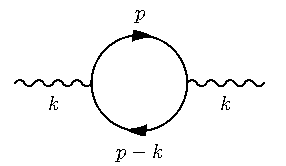
\includegraphics[scale=1.2]{图/self_photon.pdf}
 \caption{}
 \label{self_photon}
\end{figure}
此过程可看出光子将真空极化并使其生成一对正负费米子对，然后正负费米子对再湮灭产生能量相等的光子。此过程我们可以用自能表示为：
\begin{equation}
\Pi^{\mu\nu}(k)=-\int\frac{\mathrm{d}^d p}{(2\pi)^d}\sum_{\text{helicity}}(-ie_0\gamma^\mu)\frac{ i}{\slashed{p}-m}(-ie_0\gamma^\nu)\frac{ i}{\slashed{p}-\slashed{k}-m}
\end{equation}
对于内线费米子的螺旋度求和，即可以转换为旋量空间的求迹，则有：
\begin{equation}
	\Pi^{\mu\nu}(k)=-e_0^2\int\frac{\mathrm{d}^d p}{(2\pi)^d}\frac{\mathrm{tr}[\gamma^\mu(\slashed{p}+m)\gamma^\nu (\slashed{p}-\slashed{k}+m)]}{(p^2-m^2)((p-k)^2-m^2)}
\end{equation}
我们通过求迹公式，可得：
\begin{equation}
	\Pi^{\mu\nu}(k)=-4e_0^2\int\frac{\mathrm{d}^d p}{(2\pi)^d}\frac{2p^\mu p^\nu +p^\mu k^\nu+p^\nu k^\mu+(m^2-p^2-p\cdot k)\eta^{\mu\nu}}{(p^2-m^2)(p^2+2p\cdot k+k^2-m^2)}
\end{equation}
将内线动量反向\(p\rightarrow -p\)，则可利用费曼积分公式，求得：
% {\small
\begin{equation}
	\Pi^{\mu\nu}(k^2)=-4e_0^2\Big(2I^{\mu\nu}_{1,1}+k^\mu I^\nu_{1,1}+k^\nu I^\mu_{1,1}+\eta^{\mu\nu}(m^2I_{1,1}-{I^\alpha_\alpha}_{1,1}-k_\alpha I^\alpha_{1,1})\Big)
\end{equation}%}
其中
\begin{equation}
    \Omega=m^2+(x^2-x)k^2
\end{equation}
对于内部指标缩并的项${I^\alpha_\alpha}_{1,1}$，度规缩并为$\eta_{\mu\nu}\eta^{\mu\nu}=d=4-\epsilon$，再利用性质$x\Gamma(x)=\Gamma(x+1)$，可得其中一部分为：
\begin{equation}
    2I^{\mu\nu}_{1,1}-\eta^{\mu\nu}{I^\alpha_\alpha}_{1,1}=\frac{i}{(4\pi)^2}\int_0^1\mathrm{d}x\left(\frac{\Omega}{4\pi}\right)^{-\frac{\epsilon}{2}}\Gamma(\frac{\epsilon}{2})[x^2(2k^\mu k^\nu-\eta^{\mu\nu}k^2)-\eta^{\mu\nu}\Omega]
\end{equation}
然后可得另一部分：
\begin{equation}
    k^\mu I^\nu_{1,1}+k^\nu I^\mu_{1,1}-\eta^{\mu\nu}k_\alpha I^\alpha_{1,1} = -\frac{i}{(4\pi)^2}\Gamma(\frac{\epsilon}{2})\int_0^1\mathrm{d}x \;x \left(\frac{\Omega}{4\pi}\right)^{-\frac{\epsilon}{2}}(2k^\mu k^\nu-\eta^{\mu\nu}k^2)
\end{equation}
综合可得：
% {\small
\begin{equation}
    \Pi^{\mu\nu}(k)=-4e_0^2\frac{i}{(4\pi)^2}\Gamma(\frac{\epsilon}{2})\int_0^1\mathrm{d}x\left(\frac{\Omega}{4\pi}\right)^{-\frac{\epsilon}{2}}\Big[(x^2-x)(2k^\mu k^\nu-\eta^{\mu\nu}k^2)+\eta^{\mu\nu}(m^2-\Omega)\Big]
\end{equation}%}
代入$\Omega$以及$e_0=e\mu^\frac{\epsilon}{2}$，得光子自能：
\begin{equation}
    \Pi^{\mu\nu}(k)=\frac{ie^2}{2\pi^2}\left(\eta^{\mu\nu}-\frac{k^\mu k^\nu}{k^2}\right)\Gamma(\frac{\epsilon}{2})\int_0^1\mathrm{d}x\left(\frac{\Omega}{4\pi\mu^2}\right)^{-\frac{\epsilon}{2}}(\Omega-m^2)
\end{equation}
我们很容易看出，光子自能包含了横向投影的部分，因此有：
\begin{equation}
k_\mu \Pi^{\mu\nu}(k^2)=0
\end{equation}
这意味着即使考虑高阶修正光子也依然保持横向极化，使得光子并没有带上额外的质量。

再令$\epsilon$趋于0，可得：
% {\small
\begin{equation}
    \Pi^{\mu\nu}(k)={ie^2}k^2\left(\eta^{\mu\nu}-\frac{k^\mu k^\nu}{k^2}\right)\left(-\frac{1}{6\pi^2\epsilon}+\frac{1}{12\pi^2}\ln\frac{e^\gamma}{4\pi}-\frac{1}{2\pi^2}\int_0^1\mathrm{d}x(x-1)x\ln\frac{\Omega(x)}{\mu^2}\right)
\end{equation}%}

我们有裸光子场的2点格林函数\(D_{\mu\nu}\sim\langle0|{{A_0}_\mu}{A_0}_\nu|0\rangle\)，因此我们可得重整化2点光子场格林函数：
\begin{equation}
    D^r_{\mu\nu}(k)=\frac{1}{Z_A}\left[D_{\mu\nu}+D_{\mu\alpha}\Pi^{\alpha\beta}(k^2, e^2)D_{\beta\nu}+\mathcal{O}(e^4)+\cdots\right]
\end{equation}
由于光子自能可写成：
\begin{equation}
    \Pi^{\alpha\beta}(k^2, e^2)={ie^2}k^2\left(\eta^{\alpha\beta}-\frac{k^\alpha k^\beta}{k^2}\right)\Pi(k^2,\mu)
\end{equation}
那么我们可以使用朗道规范，光子传播子则为$D_{\mu\nu}=\frac{-i}{k^2}(\eta_{\mu\nu}-\frac{k_\mu k_\nu}{k^2})$。利用横向投影算符的性质，我们也可以将光子场格林函数也可写成几何级数形式：
\begin{align}
    D^r_{\mu\nu}(k)=&\frac{1}{Z_A}\frac{-i}{k^2}\left(\eta_{\mu\nu}-\frac{k_\mu k_\nu}{k^2}\right)\sum_{n=0}\left(e^2\Pi(k^2,\mu)\right)^n\notag\\
    &=\frac{1}{Z_A[1-e^2\Pi(k^2,\mu)]}\frac{-i}{k^2}\left(\eta_{\mu\nu}-\frac{k_\mu k_\nu}{k^2}\right)
\end{align}
令光子场重整化系数为$Z_A=1+\delta_A$，若使用最小差值方案重整化，那么我们可得：
\begin{equation}
    \delta_A=-\frac{e^2}{6\pi^2\epsilon}
\end{equation}
即：
\begin{equation}
    A_0^\mu=A^\mu\left(1-\frac{2\alpha}{3\pi\epsilon}\right)^\frac{1}{2}
\end{equation}
%带入回到光子传播子中
%\begin{equation}
%    D^r_{\mu\nu}(k)=\frac{-i}{k^2}\left(\eta_{\mu\nu}-\frac{k_\mu k_\nu}{k^2}\right)\left(1+\frac{e^2}{12\pi^2}\ln\frac{e^\gamma}{4\pi}-\frac{e^2}{2\pi^2}\int_0^1\mathrm{d}x(x-1)x\ln\frac{m^2+x(x-1)k^2}{\mu^2} \right)
%\end{equation}


%对于光子传播子，我们可以对其作傅里叶变换

\subparagraph{QED中的$\beta$函数}
由于我们已经得到了光子场重整化系数$Z_A$，我们可以通过Ward恒等式得到电荷重整化系数$Z_e=1/\sqrt{Z_A}$，最终我们解出QED中所有的重整化系数：
\begin{equation}
    Z_\psi=1-\frac{e^2}{8\pi^2\epsilon},\qquad Z_A=1-\frac{e^2}{6\pi^2\epsilon}, \qquad Z_m =1-\frac{3e^2}{8\pi^2\epsilon}, \qquad Z_e=1+\frac{e^2}{12\pi^2\epsilon}
\end{equation}

那么裸电荷表为：
\begin{equation}
    e_0= e\mu^{\frac{\epsilon}{2}}Z_e=e\mu^{\frac{\epsilon}{2}}\left(1+\frac{e^2}{12\pi^2\epsilon}\right)
\end{equation}
考虑：
\begin{equation}
    0=\mu\frac{\mathrm{d}}{\mathrm{d}\mu}e_0=\mu\frac{\mathrm{d}e}{\mathrm{d}\mu}\mu^{\frac{\epsilon}{2}}\left(1+\frac{e^2}{12\pi^2\epsilon}\right)+e\frac{\epsilon}{2}\mu^{\frac{\epsilon}{2}}\left(1+\frac{e^2}{12\pi^2\epsilon}\right)+\mu^{\frac{\epsilon}{2}}\frac{e^2}{6\pi^2\epsilon}\mu\frac{\mathrm{d}e}{\mathrm{d}\mu}
\end{equation}
那么最终另$\epsilon\rightarrow0$，我们可求解得QED的$\beta(e)$函数：
\begin{equation}
    \beta(e)=\mu\frac{\mathrm{d}e}{\mathrm{d}\mu}=\frac{e^3}{12\pi^2}
\end{equation}
则QED的跑动耦合常数即为：
\begin{equation}
    e^2(\mu)=\frac{e_\Lambda^2}{1-\frac{e_\Lambda^2}{6\pi^2}\ln\frac{\mu}{\Lambda}}
\end{equation}
或写为跑动精细结构常数：
\begin{equation}
    \alpha(\mu)=\frac{\alpha_\Lambda}{1-\frac{2\alpha_\Lambda}{3\pi}\ln\frac{\mu}{\Lambda}}
\end{equation}
由于QED的$\beta$-函数大于0，因此在低能标处QED不会出现渐近自由的现象，而在高能标时QED则会出现朗道极点。由我们现有的实验可知，在能标处于电子质量这个尺度的时候，精细结构常数大约是$\frac{1}{137}$。那么以此推算，我们可得QED朗道极点的能标大约为$\Lambda_\text{QED}\sim m_e e^{204\pi}\approx10^{283}$ eV。可以看出在目前实验观测范围内，所处的能标离$\Lambda_\text{QED}$还非常的遥远，因此在QED中使用微扰展开基本不会出现问题，同时该结果也符合我们对电磁相互作用的直觉。

%\subsection{QED红外发散}
\subparagraph{电子反常磁矩}
在之前的讨论中，我们已经对电磁相互作用的耦合常数进行了重整化。然而这并不代表电磁相互作用中的高阶效应已经考虑完备，实际上我们还需要考虑来自电子内部自旋的量子修正。那么我们知道电子参与相互作用时，其自旋的性质表现在磁矩上，因此电子的磁矩将会受到量子修正的影响。而有经典电动力学可知，磁矩由电流决定。则我们考虑如下电子流，中途外部电磁场于其发生相互作用的情形，而其单圈级别的作用过程可描述为费曼图~\ref{anomalous_mag}。
\begin{figure}[h]
\centering
% \begin{fmffile}{anomalous_mag}
%       \begin{fmfgraph*}(80,100)
%     \fmfleft{x2,x1}
%     \fmfright{x3}
%     \fmf{boson,t=1,label=$~~~~~~k$}{x3,v}
%     \fmf{fermion,label=$p_1$}{x2,v1}
%     \fmf{plain,t=1.3,label=$\!\!p_1-q$}{v1,v}
%         \fmf{plain,t=1.3,label=$\!\!p_2-q$}{v,v2}
%     \fmf{fermion,label=$p_2$}{v2,x1}
%         \fmffreeze
%     \fmf{boson,left=0.36,label=$q$,l.s=left}{v1,v2}
%   \end{fmfgraph*}
% \end{fmffile}
    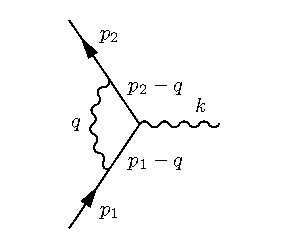
\includegraphics[scale=1.3]{图/anomalous_mag.pdf}
    \caption{}
    \label{anomalous_mag}
\end{figure}
那么该单圈电子流在费曼规范下可表示为：
% {\small
\begin{equation}
    J_{(1)}^\mu=\bar{u}(p_2)\Bigg[\int\frac{\mathrm{d}^4q}{(2\pi)^4}(-ie_0\gamma^\beta)\frac{i}{\slashed{p}_2-\slashed{q}-m}(-ie_0\gamma^\mu)\frac{i}{\slashed{p}_1-\slashed{q}-m}(-i_0e\gamma^\alpha)\frac{-i\eta_{\alpha\beta}}{q^2}\Bigg]u(p_1)
\end{equation}%}
此时考虑单圈级别的电流可以表示为$J_{(1)}^\mu=-ie_0\bar{u}(p_2)\Gamma_{(1)}^\mu u(p_1)$的普适形式，那么只考虑中间的顶点函数部分：
% {\small
\begin{align}
    \Gamma_{(1)}^\mu=&-ie_0^2\int\frac{\mathrm{d}^dq}{(2\pi)^d}\frac{\gamma_a(\slashed{p}_2-\slashed{q}+m)\gamma^\mu(\slashed{p}_1-\slashed{q}+m)\gamma^\alpha}{q^2[(p_2-q)^2-m^2][(p_1-q)^2-m^2]}\notag\\
    =&-ie_0^2\int\frac{\mathrm{d}^dq}{(2\pi)^d}\frac{[2(p_2-q)_\alpha-(\slashed{p}_2-m-\slashed{q})\gamma_\alpha]\gamma^\mu[2(p_1-q)^\alpha-\gamma^\alpha(\slashed{p}_1-m-\slashed{q})]}{q^2[(p_2-q)^2-m^2][(p_1-q)^2-m^2]}
\end{align}%}
由于考虑外线电子为是实的在壳电子，则有$\slashed{p}_2-m=0$，$\slashed{p}_1-m=0$，且考虑动量$q$反向，可得：
\begin{equation}
    \Gamma_{(1)}^\mu=-ie_0^2\int\frac{\mathrm{d}^dq}{(2\pi)^d}\frac{(2(p_2+q)_\alpha-\slashed{q}\gamma_\alpha)\gamma^\mu(2(p_1+q)^\alpha-\gamma^\alpha \slashed{q})}{q^2[q^2+2q\cdot p_2+p_2^2-m^2][q^2+2q\cdot p_1+p_1^2-m^2]}\notag\\
    %=e^2\int\frac{\mathrm{d}^dq}{(2\pi)^d}\frac{}{q^2[(p_2+q)^2-m^2][(p_1+q)^2-m^2]}
\end{equation}
对于分子部分，我们利用$\gamma_\alpha\gamma^\mu\gamma^\alpha=(2-d)\gamma^\mu$，且利用反对易关系，有：
% {\small
\begin{align}
&(2(p_2+q)_\alpha-\slashed{q}\gamma_\alpha)\gamma^\mu(2(p_1+q)^\alpha-\gamma^\alpha \slashed{q})\notag\\
    =&4\gamma^\mu(p_2+q)\cdot(p_1+q)-2\slashed{q}\gamma_\alpha\gamma^\mu(p_1+q)^\alpha-2(p_2+q)_\alpha\gamma^\mu\gamma^\alpha \slashed{q}+\slashed{q}\gamma_\alpha\gamma^\mu\gamma^\alpha \slashed{q}\notag\\
    =&4\gamma^\mu(p_2+q)\cdot(p_1+q)-4q^2\gamma^\mu-2\slashed{q} \slashed{p}_1\gamma^\mu-2\gamma^\mu \slashed{p}_2\slashed{q}+2(2-d)\slashed{q} q^\mu-(2-d)q^2 \gamma^\mu\notag\\
    =&\gamma^\mu [4(p_2\cdot p_1 + p_2\cdot q +q\cdot p_1)-(2-d)q^2]+2(2-d)\slashed{q} q^\mu-2\slashed{q} \slashed{p}_1\gamma^\mu-2\gamma^\mu \slashed{p}_2\slashed{q}\notag\\
    =&\gamma^\mu [4p_2\cdot p_1 + 4q\cdot(p_2 + p_1)-(2-d)q^2]+2(2-d)\slashed{q} q^\mu+4m q^\mu-4\slashed{q}(p_1+p_2)^\mu\notag\\
    =&4\gamma^\mu p_1\cdot p_2 + 4q^\nu[\gamma^\mu(p_1+p_2)_\nu-\gamma_\nu(p_1+p_2)^\mu+{m}\delta_\nu^\mu]+(2-d)q^\nu q^\rho[2\gamma_\rho\delta_\nu^\mu-\gamma^\mu\eta_{\nu\rho}] 
\end{align}%}
那么代入回积分中，我们可以引用费曼积分将其写为：
\begin{multline}
        \Gamma_{(1)}^\mu=-ie_0^2\Big[4\gamma^\mu p_1\cdot p_2 I_{1,1,1}+ 4I_{1,1,1}^\nu[\gamma^\mu(p_1+p_2)_\nu-\gamma_\nu(p_1+p_2)^\mu+{m}\delta_\nu^\mu]\\+(2-d)I_{1,1,1}^{\nu\rho}[2\gamma_\rho\delta_\nu^\mu-\gamma^\mu\eta_{\nu\rho}]    \Big]
\end{multline}
由于其中的单圈积分$I_{1,1,1}\sim \int\frac{\mathrm{d}q}{q^3}$，那么可以预见当内线动量$q\rightarrow0$时，圈积分则会出现发散。此时情况不同于内线动量$p\rightarrow\infty$时出现的发散，因此我们称之为\emph{红外发散}。

我们可以通过费曼积分公式，计算得：
% {\footnotesize
\begin{align}
I_{1,1,1}=&-\frac{i}{32\pi^2}\int_0^1\frac{\mathrm{d}x}{\Delta(x)}\ln\frac{\Delta(x)}{\epsilon^2}+\mathcal{O}(\epsilon),\qquad I_{1,1,1}^\mu=(p_1+p_2)^\mu\frac{i}{32\pi^2}\int_0^1\frac{\mathrm{d}x}{\Delta(x)}\\
I_{1,1,1}^{\mu\nu}=&\frac{i\eta^{\mu\nu}}{32\pi^2}\int_0^1 u\,\mathrm{d}u\int_0^1 x\,\mathrm{d}x\;\Gamma(\frac{\epsilon}{2})\left(\frac{u^2\Delta(x)}{4\pi}\right)^{-\frac{\epsilon}{2}}\notag\\&-\frac{i}{128\pi^2}\Big[(p_1+p_2)^\mu(p_1+p_2)^\nu\int_0^1\frac{\mathrm{d}x}{\Delta(x)}+(p_1-p_2)^\mu(p_1-p_2)^\nu\int_0^1\frac{x^2\mathrm{d}x}{\Delta(x)}\Big]
%\begin{split}
%
%\end{split}
\end{align}%}
%\frac{\eta^{\mu\nu}}{(d-2)^2\mu^\epsilon}\Big[\frac{i}{8\pi^2\epsilon}-\frac{i}{16\pi^2}\Big(\int_0^1\mathrm{d}x\ln\frac{\Omega(x)}{\mu^2}+\ln\frac{e^\gamma}{4\pi}\Big)+\mathcal{O}(\epsilon)\Big]
其中:
\begin{equation}
\Delta(x)=m^2-\frac{1}{4}(1-x^2)k^2,\qquad k^\mu=p^\mu_2-p^\mu_1
\end{equation}

此时对于两个外线电子而言，我们有狄拉克方程$(\slashed{p}_1-m)u(p_1)=0$，$\bar{u}(p_2)(\slashed{p}_2-m)=0$，可得：
\begin{align}
m\gamma^\mu u(p_1)=\gamma^\mu\gamma^\nu {p_1}_\nu u(p_1) =(p_1^\mu-i\sigma^{\mu\nu}{p_1}_\nu)u(p_1)\\
m \bar{u}(p_2)\gamma^\mu=\bar{u}(p_2){p_2}_\nu\gamma^\nu\gamma^\mu   =\bar{u}(p_2)(p_2^\mu+i\sigma^{\mu\nu}{p_2}_\nu)
\end{align}
然后在上式1式的左侧乘上$\bar{u}(p_2)$，在上式2式的右侧乘上$u(p_1)$，再将两式相加可得：
\begin{equation}
\bar{u}(p_2)\gamma^\mu u(p_1)=\bar{u}(p_2)\Big(\frac{(p_1+p_2)^\mu}{2m}-\frac{i\sigma^{\mu\nu}}{2m}(p_1-p_2)_\nu\Big) u(p_1)
\end{equation}
此式称为Gordon恒等式。通过此式我们可得：
\begin{equation}
(p_1+p_2)^\mu=2m\gamma^\mu +i\sigma^{\mu\nu}(p_1-p_2)_\nu
\end{equation}

综合以上结果，再带入回电流中的顶点函数项，我们可得：
\begin{multline}
\Gamma_{(1)}^\mu=e^2\Big[ \frac{i\sigma^{\mu\nu}}{16\pi^2}k_\nu\int_0^1\frac{\mathrm{d}x}{\Delta(x)}+\gamma^\mu\Big(\frac{1}{8\pi^2\epsilon}-\frac{p_1\cdot p_2}{8\pi^2}\int_0^1\frac{\mathrm{d}x}{\Delta(x)}\ln\frac{\Delta(x)}{\epsilon^2}\\
-\frac{1}{16\pi^2}\int_0^1\mathrm{d}x\ln\frac{\Delta(x)e^\gamma}{4\pi\mu^2}+\frac{p_1\cdot p_2}{32\pi^2}\int_0^1\frac{7+x^2}{\Delta(x)}\mathrm{d}x+\frac{m^2}{32\pi^2}\int_0^1\frac{x^2-3}{\Delta(x)}\mathrm{d}x\Big)
\Big]\label{eq:1lvertex}
\end{multline}
由上式的结果不难看出，顶点函数包含两个具有不同螺旋度结构的部分，因此对于电磁相互作用的顶点函数，可以表为：
\begin{equation}
    \Gamma^\mu=\gamma^\mu+\Gamma_{(1)}^\mu+\cdots=F_e\gamma^\mu+F_m\frac{i\sigma^{\mu\nu}}{2m}k_\nu
\end{equation}
其中$F_e$为电子的电形状因子，而$F_m$为电子的磁形状因子。
对于电形状因子部分，则需要进行重整化。由\eqref{eq:wardf}式Ward恒等式可知：
\begin{equation}
    \Gamma^\mu_r=Z_\psi\Gamma^\mu
\end{equation}
带入\eqref{eq:qedferren}的结果，可得：
\begin{align}
        \Gamma^\mu_r&=\Big(1-\frac{e^2}{8\pi^2\epsilon}\Big)(\gamma^\mu+F^{(1)}_e\gamma^\mu+\cdots)=\gamma^\mu+(F^{(1)}_e-\frac{e^2}{8\pi^2\epsilon})\gamma^\mu+\mathcal{O}(e^4)+\cdots
\end{align}
则可得重整化电形状因子：
\begin{multline}
            {F_e}_r=1+\frac{\alpha}{2\pi}\Big(\frac{p_1\cdot p_2}{4}\int_0^1\frac{7+x^2}{\Delta(x)}\mathrm{d}x+\frac{m^2}{4}\int_0^1\frac{x^2-3}{\Delta(x)}\mathrm{d}x-\frac{1}{2}\int_0^1\mathrm{d}x\ln\frac{\Delta(x)e^\gamma}{4\pi\mu^2}\\\hspace{1cm}-{p_1\cdot p_2}\int_0^1\frac{\mathrm{d}x}{\Delta(x)}\ln\frac{\Delta(x)}{\epsilon^2}\Big)+\mathcal{O}(\alpha^2)+\cdots
\end{multline}
我们注意到此时的重整化只能将电形状因子中的紫外发散部分消去，而其中红外发散项依然存在。实际上如果只单独考虑这样的过程，是无法将红外发散消除的。而在实际中当靠近红外能区时，电磁相互作用过程还会有轫制辐射过程，其也会产生红外发散。而最终，轫制辐射中的红外发散项与电形状因子中的红外发散项相互抵消，才使得相互作用过程的可观测量能保持有限。

而对于磁形状因子，我们可以考虑\eqref{eq:1lvertex}式的$\sigma^{\mu\nu}$项，其中积分项取近似$\int_0^1\frac{\mathrm{d}x}{\Omega(x)}\sim\frac{1}{m^2}$，则可得首阶的磁形状因子：
\begin{equation}
    F^{(0)}_m=\frac{\alpha}{2\pi}
\end{equation}

由于现在我们知道电磁相互作用顶点函数可以包含两种螺旋度结构，因此我们考虑将上述顶点函数带入\eqref{eq:effvert}式，则可得关于电磁相互作用部分的有效作用量：
\begin{multline}
    \bar{\Gamma}_\text{int}=\int\mathrm{d}x_1\mathrm{d}x_2\mathrm{d}x\int\mathrm{d}p_1\mathrm{d}p_2\mathrm{d}k\;\delta(p_1-p_2+k)e^{i(p_1x_1-p_2x_2+kx)}\\\times\Big[\bar{\psi}(x_2)\Big(F_e(k)\gamma^\mu+F_m(k)\frac{i\sigma^{\mu\nu}}{2m}k_\nu\Big)A_\mu(x)\psi(x_1)\Big]
\end{multline}
将$p_1$，$p_2$，$x_2$积分掉，可得：
\begin{equation}
    \bar{\Gamma}_\text{int}=\int\mathrm{d}x_1\mathrm{d}x\int\mathrm{d}k\;\Big[\bar{\psi}(x_1)\Big(F_e(k)\gamma^\mu+F_m(k)\frac{\sigma^{\mu\nu}}{2m}k_\nu\Big)e^{ik(x-x_1)}A_\mu(x)\psi(x_1)\Big]
\end{equation}
此时利用$e^{ikx}$可以将函数中的$ik_\mu$替换为对右侧$e^{ikx}$的导数$\partial_\mu$，可得：
\begin{align}
      \bar{\Gamma}_\text{int}&=\int\mathrm{d}x_1\mathrm{d}x\int\mathrm{d}k\;\Big[\bar{\psi}(x_1)\Big(F_e(\partial)\gamma^\mu+F_m(\partial)\frac{\sigma^{\mu\nu}}{2m}\partial_\nu\Big)e^{ik(x-x_1)}A_\mu(x)\psi(x_1)\Big]\notag\\
      &=\int\mathrm{d}x_1\mathrm{d}x\;\delta(x-x_1)\Big[\bar{\psi}(x_1)\Big(F_e(\partial)\gamma^\mu A_\mu(x)+F_m(\partial)\frac{\sigma^{\mu\nu}}{2m}\partial_\nu A_\mu(x)\Big)\psi(x_1)\Big]\notag\\
      &=\int\mathrm{d}x\;\bar{\psi}(x)\Big(F_e(\partial)\gamma^\mu A_\mu(x)-F_m(\partial)\frac{\sigma^{\mu\nu}}{4m}F_{\mu\nu}(x)\Big)\psi(x)
\end{align}
其中利用了$\sigma^{\mu\nu}$的反对称性质。

此时我们考虑树图层面的电形状因子以及单圈层面的磁形状因子，那么QED的有效作用量则可以表示为：
\begin{equation}
  \bar{\Gamma}_\text{QED}=\int\mathrm{d}x \Bigg[\bar{\psi}(i\slashed{\partial}-m)\psi-\frac{1}{4}F^{\mu\nu}F_{\mu\nu}-e\bar{\psi}\Big(\slashed{A}-\frac{\alpha}{8\pi m}\sigma^{\mu\nu}F_{\mu\nu}\Big)\psi\Bigg]  
\end{equation}
那么此时关于电子的运动方程则为：
\begin{equation}
    \Big(\gamma^\mu(i\partial_\mu-eA_\mu)-m+\frac{e^3}{32\pi^2 m}\sigma^{\mu\nu}F_{\mu\nu}\Big)\psi=0
\end{equation}
我们可将上式化成薛定谔方程的形式，则有：
\begin{equation}
    i\frac{\partial}{\partial t} \psi=\Bigg[\alpha_i\Big(i\partial_i-e A_i\Big)+eA_0+m\gamma^0 -\mu_\text{B}\frac{\alpha}{2\pi}(i\boldsymbol{\alpha}\cdot\boldsymbol{E}-\boldsymbol{\Sigma}\cdot\boldsymbol{B})\Bigg] \psi
\end{equation}
其中$\mu_\text{B}=\frac{e\hbar}{2mc}$为玻尔磁子。则此时可得哈密顿量为：
\begin{equation}
    \mathcal{H}=m\gamma^0+\boldsymbol{\alpha}\cdot(\boldsymbol{p}-e\boldsymbol{A})+eA_0 -\mu_\text{B}\frac{\alpha}{2\pi}(i\boldsymbol{\alpha}\cdot\boldsymbol{E}-\boldsymbol{\Sigma}\cdot\boldsymbol{B})
\end{equation}
此时的哈密顿算符存在非对角元，也就是说该表象并不为能量本征态，因此我们将哈密顿算符进行块对角化，并且考虑低能近似，便可使运动方程回归到量子力学中的泡利方程，则其中一块的哈密顿算符为：
\begin{equation}
    \hat{\mathcal{H}}=\frac{(\boldsymbol{p}-\frac{e}{c}\boldsymbol{A})^2-(1+\frac{\alpha}{2\pi})\frac{e\hbar}{c}\boldsymbol{\sigma}\cdot\boldsymbol{B}}{2m}+eA_0-(1+\frac{\alpha}{\pi})\frac{e\hbar}{4m^2c^2}\boldsymbol{\sigma}\cdot(\boldsymbol{E}\times\boldsymbol{p})+\mathcal{O}(\hbar^2)
\end{equation}
%\\-(1+\frac{\alpha}{\pi})\frac{ie\hbar^2}{8m^2c^2}\boldsymbol{\sigma}\cdot(\nabla\times\boldsymbol{E})-\frac{e\hbar^2}{8m^2c^2}\nabla\cdot\boldsymbol{E}+\mathcal{O}(\frac{1}{m^3})
当外磁场为匀强磁场时，则有$\boldsymbol{A}=\frac{1}{2}\boldsymbol{B}\times\boldsymbol{r}$，而同时没有涡旋电场，则$\nabla\times\boldsymbol{E}=0$，$\boldsymbol{E}=-\nabla A_0=-\frac{\boldsymbol{r}}{r}\frac{\mathrm{d}A_0}{\mathrm{d}r}$，可得：
\begin{gather}
    (\boldsymbol{p}-\frac{e}{c}\boldsymbol{A})^2= \boldsymbol{p}^2-\frac{e}{c}\boldsymbol{L}\cdot\boldsymbol{B}+\frac{e^2}{4c^2}(\boldsymbol{B}^2\boldsymbol{r}^2-(\boldsymbol{B}\cdot\boldsymbol{r})^2)\\
    \boldsymbol{\sigma}\cdot(\boldsymbol{E}\times\boldsymbol{p})=-\frac{1}{r}\frac{\mathrm{d}A_0}{\mathrm{d}r}\boldsymbol{\sigma}\cdot\boldsymbol{L}
\end{gather}
我们知道自旋角动量的定义为$\boldsymbol{s}=\frac{\hbar}{2}\boldsymbol{\sigma}$，综合上述结果，我们可得：
\begin{equation}
    \hat{\mathcal{H}}=\frac{p^2}{2m}+eA_0-\frac{e}{2mc}\left(\boldsymbol{L}+2\big(1+\frac{\alpha}{2\pi}\big)\boldsymbol{s} \right) \cdot\boldsymbol{B}-\frac{e}{2m^2c^2}\left(1+\frac{\alpha}{\pi}\right)\boldsymbol{s}\cdot\boldsymbol{L}
\end{equation}
我们可以从上式得出电子的自旋磁矩为：
\begin{equation}
    \boldsymbol{\mu}_s=g \frac{\mu_\text{B}}{\hbar}  \boldsymbol{s}=2\left(1+\frac{\alpha}{2\pi}\right)\frac{\mu_\text{B}}{\hbar}  \boldsymbol{s}
\end{equation}
此时朗德因子$g=2\left(1+\frac{\alpha}{2\pi}\right)\approx2.0023$，此结果与实验相符合。而上式最后一项即为自旋轨道耦合作用项。

对比量子力学中的结果不难看出，在不考虑单圈修正所带来的磁形状因子项的影响，朗德因子即为$g=2$。而自旋磁矩中$g=2$以外的部分则称为反常磁矩，其表示了场论的高阶修正对于电子自旋磁矩影响$a=\frac{g-2}{2}$。因此，量子电动力学的高阶修正项更加精确的描述了电子自旋磁矩以及电子的自旋轨道耦合项，使得理论计算更加地符合实验结果，同时这也成为了量子电动力学强有力的证据。

% \subparagraph{软光子轫制辐射}
% Pauli-Villars正规化

\chapter{杨-Mills场理论}
\section{Non-Abliean规范场}
考虑参与该相互作用的物质场满足内禀局域SU($N$)对称性，此时规范群元互不对易，则规范场$A_\mu$为Non-Abliean规范场，也称为杨-Mills场。此时：
\begin{equation}
	U(x)=e^{i\omega^a(x)\boldsymbol{T}^a}
\end{equation}
对于SU($N$)变换的无穷小表象$U(x)\approx1+i\omega^a(x)\boldsymbol{T}^a$，由式\eqref{eq:gaugetr}，矢量场$A_\mu$的规范变换为：
\begin{equation}
	A_\mu\rightarrow A_\mu+\frac{1}{g}\boldsymbol{T}^a\partial_\mu \omega^a(x)+i\omega^a(x)[\boldsymbol{T}^a,A_\mu]+\mathcal{O}(\omega^2)
\end{equation}
矢量场场$A_\mu$可表示为：
\begin{equation}
A_\mu(x)=A^a_\mu(x)\boldsymbol{T}^a
\end{equation}
而$\omega^a\boldsymbol{T}^a=\boldsymbol{\omega}$，则规范场$A_\mu$的无穷小变换可表示为\footnote{对$\boldsymbol{\omega}$的协变导数表示为：\[\begin{split}
	D_\mu\boldsymbol{\omega}&=\partial_\mu\omega^c\boldsymbol{T}^c-igA_\mu^a(if^{abc}\omega^b)\boldsymbol{T}^c\\&=\partial_\mu\omega^c\boldsymbol{T}^c-igA_\mu^a\omega^b[\boldsymbol{T}^a,\boldsymbol{T}^b]\\&=\partial_\mu\boldsymbol{\omega}-ig[A_\mu,\boldsymbol{\omega}]
	\end{split}\]即\[D_\mu\omega^a=\partial_\mu\omega^a-gf^{abc}\omega^b A_\mu^c\]}：
\begin{equation}
\begin{split}
\delta A_\mu&=\frac{1}{g}\partial_\mu\boldsymbol{\omega}-i[A_\mu,\boldsymbol{\omega}]\\
&=\frac{1}{g}D_\mu\boldsymbol{\omega}
\end{split}
\end{equation}
利用生成元$\boldsymbol{T}^a$的性质，并忽略高阶项，我们可得：
\begin{equation}
\begin{split}
	A^a_\mu\rightarrow& A^a_\mu+\frac{1}{g}\partial_\mu \omega^a(x)-f^{abc}\omega^b(x)A^c_\mu\\&=A^a_\mu+\frac{1}{g}D_\mu\omega^a(x)
\end{split}
\end{equation}
由于此时场$A_\mu$为Non-Abliean，即场之间不再对易。

对于场强张量$F_{\mu\nu}=F^a_{\mu\nu}\boldsymbol{T}^a$，我们有：
\begin{equation}
	F^a_{\mu\nu}=\partial_\mu A^a_\nu-\partial_\nu A^a_\mu+gf^{abc}A^b_\mu A^c_\nu
\end{equation}
则场强的规范变换为：
\begin{align}
F_{\mu\nu}\rightarrow F'_{\mu\nu}&= UF_{\mu\nu}U^\dagger\notag\\
&= F_{\mu\nu}-f^{abc}\omega^a F_{\mu\nu}^b \boldsymbol{T}^c
\end{align}

对于杨-Mills场，我们需要构造规范不变的Lagrangian动能项。因此可以利用求迹消去规范变换产生的额外项，则最终杨-Mills场动能项为\footnote{除以上表示方式外，规范场还有另一种表示，即将$i$和$g$分别缩并到规范群生成元和场函数中，两种表示的相互关系可以表为$\boldsymbol{T}^a\rightarrow i\boldsymbol{T}^a, A^a_\mu\rightarrow gA^a_\mu$，则可以将规范场表示为更规整的形式：
	\[\begin{split}
		&[\boldsymbol{T}^a,\boldsymbol{T}^b]=f^{abc}\boldsymbol{T}^c,\qquad\mathrm{tr}(\boldsymbol{T}^a\boldsymbol{T}^b)=-\frac{1}{2}\delta^{ab}\\
	&D_\mu=\partial_\mu+A_\mu,\qquad\qquad F_{\mu\nu}=[D_\mu,D_\nu]=\partial_\mu A_\nu-\partial_\nu A_\mu+[A_\mu,A_\nu]\\
	&\mathscr{L}_{\text{YM}}^{\text{kin}}=\frac{1}{g^2}\mathrm{tr}(F_{\mu\nu}F^{\mu\nu}),
	\end{split}\]	]}：
\begin{equation}
	\mathscr{L}_{\text{YM}}^{\text{kin}}=-\frac{1}{2}\mathrm{tr}(F_{\mu\nu}F^{\mu\nu})=-\frac{1}{4}F^a_{\mu\nu}{F^a}^{\mu\nu}
\end{equation}
这样的动能项即可以保证Lagrangian的洛伦兹不变性，也可以保证规范不变性。

考虑费米子参与相互作用，则Lagrangian为：
\begin{equation}
\mathscr{L}_{\text{YM}}=-\frac{1}{4}F^a_{\mu\nu}{F^a}^{\mu\nu}+\bar{\psi}(i\slashed{D}-m)\psi
\end{equation}
对矢量场取变分则可得运动方程：
\begin{equation}
\partial_\mu {F^a}^{\mu\nu}+gf^{abc}A^b_\mu {F^c}^{\mu\nu}=-g\bar{\psi}\gamma^\nu\boldsymbol{T}^a\psi
\end{equation}
\section{Faddeev-Popov量子化}
对于杨-Mills场的作用量而言，其必须具有规范对称性。因此对于规范群中的两个用规范变换联系的场函数，其描述的作用量必然是相同的。
\begin{equation}
	\mathcal{S}[A_\mu]=\mathcal{S}[A_\mu^U],\qquad A_\mu^U=U A_\mu U^\dagger+\frac{i}{g}U(\partial_\mu U)
\end{equation}
而当我们考虑路径积分$Z$时，往往会将整个规范空间的所有场都求了和，导致重复的计算了路径积分。因此我们在求格林函数生产泛函的时候，必须考虑扣除对规范空间的积分。

在之前对矢量场的讨论中，我们往往是固定了某个规范之后，再进行计算，实际上即为扣除多余规范空间自由度。因此，此时我们也需要固定一个规范条件，可以定义一系列广义的规范条件：
\begin{equation}
	\varphi^a(A_\mu)=0
\end{equation}
此时，为了扣除对规范空间的路径积分，我们可以定义一个测度上的抵消量$\Delta[A_\mu]$，其表示单独地对规范空间的路径积分：
\begin{equation}
	\frac{1}{\Delta[A_\mu]}=\int\mathcal{D}U\prod_a\delta(\varphi^a(A_\mu^U))
\end{equation}
其中还加上规范条件的约束，使得$\Delta[A_\mu]$整体规范不变。那么这时，路径积分可表为：
\begin{equation}
	\begin{split}
		Z=&\int\mathcal{D}A_\mu e^{i\mathcal{S}[A_\mu]}\\
		=&\int\mathcal{D}A_\mu\mathcal{D}U\prod_a\delta(\varphi^a(A_\mu^U))\Delta[A_\mu] e^{i\mathcal{S}[A_\mu]}\\
		=&\int\mathcal{D}U\prod_a\int\mathcal{D}A_\mu^a\delta(\varphi^a(A_\mu))\Delta[A_\mu] e^{i\mathcal{S}[A_\mu]}
	\end{split}
\end{equation}
通过交换积分次序，我们可以将对规范空间的路径积分分离出来，得到对于特定规范条件下的路径积分：
\begin{equation}
	Z=\int\mathcal{D}A_\mu^a\delta(\varphi^a(A_\mu))\Delta[A_\mu] e^{i\mathcal{S}[A_\mu]}
\end{equation}
这便是真正具有物理意义的规范场路径积分。

然而对于抵消量$\Delta[A_\mu]$，有：
\begin{equation}
	\frac{1}{\Delta[A_\mu]}=\int\mathcal{D}U\delta(\varphi(A_\mu))=\int\mathcal{D}\varphi\det\left|\frac{\delta U}{\delta \varphi}\right|\delta(\varphi(A_\mu))=\det\left|\frac{\delta U}{\delta\varphi}\right|_{\varphi=0}
\end{equation}
将规范变换$U=\exp(\omega^a\boldsymbol{T}^a)$代入，则可得：
\begin{equation}
	\Delta[A_\mu]^{ab}=\det\left|\frac{\delta\varphi(A_\mu)}{\delta U}\right|_{\varphi=0}=\det\left|\frac{\delta\varphi^a(A_\mu)}{\delta \omega^b}\right|_{\varphi^a=0}
\end{equation}
代入到路径积分中，可得：
\begin{equation}
	Z=\int\mathcal{D}A^a_\mu\delta(\varphi^a(A_\mu))\det\left|\frac{\delta\varphi^a(A_\mu)}{\delta \omega^b}\right|_{\varphi^a=0}e^{i\mathcal{S}[A_\mu]}
\end{equation}

对于规范条件$\varphi^a$，我们可以对其移位，而得到另一规范条件：
\begin{equation}
	{\varphi'}^a=\varphi^a-e^a
\end{equation}
那么对该规范条件的变分导数仍保持不变，但规范约束项改变。此时我们可得：
\begin{equation}
	Z=\int\mathcal{D}A^a_\mu\delta(\varphi^a(A_\mu)-e^a)\det\left|\frac{\delta\varphi^a(A_\mu)}{\delta \omega^b}\right|_{\varphi^a=0}e^{i\mathcal{S}[A_\mu]}
\end{equation}

由此，我们可得格林函数生成泛函：
\begin{equation}
	Z[J]=\int\mathcal{D}A^a_\mu\delta(\varphi^a(A_\mu)-e^a)\det\left|\frac{\delta\varphi^a(A_\mu)}{\delta \omega^b}\right|_{\varphi^a=0}e^{i\mathcal{S}[A_\mu]+i\int\mathrm{d}x {A^\mu}^aJ_\mu^a}
\end{equation}

对于规范空间的位移$e^a(x)$而言，我们可以构造路径积分：
\begin{equation}
	\int\mathcal{D}e^a\;\delta(\varphi^a-e^a)e^{-i\frac{\lambda}{2}\int\mathrm{d}x\,e^a e^a}=e^{-i\frac{\lambda}{2}\int\mathrm{d}x\,\varphi^a\varphi^a}
\end{equation}
将此额外的路径积分插入到格林函数生成泛函中仅相当于多乘一个常数，并不影响具体结果，同时这样可以帮助我们将规范条件写成作用量的约束项形式。
\begin{equation}
	Z[J]=\int\mathcal{D}A^a_\mu\det\left|\frac{\delta\varphi^a(A_\mu)}{\delta \omega^b}\right|_{\varphi^a=0}e^{i\mathcal{S}[A_\mu]-i\frac{\lambda}{2}\int\mathrm{d}x\,\varphi^a\varphi^a+i\int\mathrm{d}x {A^\mu}^aJ_\mu^a}
\end{equation}

对于规范空间的行列式项而言，我们则可由Grassmann变量的积分\eqref{eq:grassintegal}式，将此行列式项改也写为路径积分项：
\begin{equation}
	\det\left|\frac{\delta\varphi^a(A_\mu)}{\delta \omega^b}\right|=\int\mathcal{D}\bar{c}\mathcal{D}c \exp\left[{-i\int\mathrm{d}x\mathrm{d}y\;\bar{c}^a(x)\frac{\delta\varphi^a(A_\mu)}{\delta \omega^b}c^b(y)}\right]
\end{equation}
最终总的格林函数生成泛函可以写为：
\begin{gather}
	Z[J]=\int\mathcal{D}A^a_\mu\mathcal{D}\bar{c}\mathcal{D}c\;e^{i(\mathcal{S}_{\text{FP}}+\int\mathrm{d}x{A^\mu}^aJ_\mu^a)}\\
	\mathcal{S}_{\text{FP}}=\mathcal{S}[A_\mu]-\frac{\lambda}{2}\int\mathrm{d}x\;\varphi^a\varphi^a-\int\mathrm{d}x\mathrm{d}y\;\bar{ c}^a(x)\frac{\delta\varphi^a(A_\mu)}{\delta \omega^b} c^b(y)
\end{gather}
其中的Grassmann变量$ c,\bar{ c}$称为Faddeev-Popov鬼场。而$\mathcal{S}_{\text{FP}}$即为Faddeev-Popov作用量，即包含规范场的规范不变作用量和规范约束项，以及鬼场项。为了保证可观测量的厄密性，我们需要对于鬼场引入如下厄米共轭关系：
\begin{equation}
	(\bar{ c}^a)^\dagger=-\bar{ c}^a,\qquad( c^a)^\dagger= c^a
\end{equation}

若我们取洛伦兹规范，则规范条件为：
\begin{equation}
	\varphi^a=\partial^\mu A_\mu^a=0
\end{equation}
那么即有：
\begin{equation}
	\varphi^a=\partial^\mu(A_\mu^a+\frac{1}{g}D_\mu\omega^a)=0
\end{equation}
由此可计算得：
\begin{equation}
	\frac{\delta\varphi^a(A_\mu)}{\delta \omega^b}\Big|_{\varphi^a=0}=\frac{1}{g}\partial^\mu (\partial_\mu\delta^{ab}-gf^{abc}A_\mu^c)\delta(x-y)
\end{equation}
代入到作用量中，可得：
\begin{equation}
	\begin{split}
		\mathcal{S}_{\text{FP}}=&\mathcal{S}[A_\mu]-\frac{\lambda}{2}\int\mathrm{d}x\;(\partial^\mu A_\mu^a)^2-\frac{1}{g}\int\mathrm{d}x\;\bar{ c}^a\partial^\mu D_\mu c^a\\
		=&\mathcal{S}[A_\mu]-\frac{\lambda}{2}\int\mathrm{d}x\;(\partial^\mu A_\mu^a)^2-\frac{1}{g}\int\mathrm{d}x\;\Big(\bar{ c}^a\partial^\mu\partial_\mu c^a-gf^{abc}\partial^\mu A_\mu^c\bar{ c}^a  c^b\Big)
	\end{split}
\end{equation}
% 即得有效Lagrangian：
% \begin{equation}
% 	\mathscr{L}_{\text{FP}}=-\frac{1}{4}F^a_{\mu\nu}{F^a}^{\mu\nu}-\frac{\lambda}{2}(\partial^\mu A_\mu^a)^2+\frac{1}{g}\partial^\mu\bar{\theta}^a\partial_\mu\theta^a+f^{abc}\bar{\theta}^a \theta^bA_\mu^c
% \end{equation}
其中对于规范约束项而言，$\lambda=\frac{1}{\xi}$即为所谓的$R_\xi$规范。
而后两项即分别为鬼场的动能项和鬼场与杨-Mills场的相互作用项。可以看出鬼场并不具有内禀自旋结构，形式上类似于标量场，但是又具有反对易的统计属性，因此这样的粒子破坏了自旋统计定理。然而鬼场实际上并非为真实的可观测物理粒子，仅仅只是杨-Mills场规范自由度的一种体现。但另一方面，鬼场对于杨-Mills场的高阶圈图过程却有实在的贡献，因此我们也不能简单的将其忽略。

对于鬼场而言，Lagrangian可以在如下全局变换下爆出不变
\begin{equation}
    \bar{c}^a\rightarrow\bar{c}^a e^\alpha,~~~~c\rightarrow c\, e^{-\alpha}
\end{equation}
则我们可得该全局对称性对应的Nöther流
\begin{equation}
    J^\mu _\text{ghost} = \partial^\mu \bar{c}^a c^a-\bar{c}^aD^\mu c^a
\end{equation}
则其对应的守恒荷即为“鬼数”:
\begin{equation}
    N_\text{ghost} = \int\mathrm{d}^3\boldsymbol{x}(\partial_0 \bar{c}^a\, c^a - \bar{c}^a D_0c^a)
\end{equation}

我们考虑具体的规范场费曼规则。对于规范场的传播子，我们可以从生成泛函中的动能项获得：
\begin{align}
	Z_A[J]=&\int\mathcal{D}A_\mu\,\exp\Big( i\int\mathrm{d}x\Big[\frac{1}{2}A_\mu^a(\eta^{\mu\nu}\partial_\lambda \partial^\lambda-(1-\frac{1}{\xi})\partial^\mu\partial^\nu)A_\nu^b\delta^{ab}+A_\mu^a {J^a}^\mu\Big]	\Big)\notag\\
	=&\int\mathcal{D}A_\mu\,\exp\Big( i\int\mathrm{d}x\Big[\frac{1}{2}A_\mu^a {D^{\mu\nu}}^{ab} A_\nu^b+A_\mu^a {J^\mu}^a\Big]	\Big)\notag\\
	=&\exp\Big(-\frac{i}{2}\int\mathrm{d}x\mathrm{d}y {J(x)^\mu}^a D_{\mu\nu}^{ab}(x-y) {J(y)^\nu}^b\Big)
\end{align}
易得，规范场传播子在$R_\xi$规范下即为：
\begin{equation}
	D_{\mu\nu}^{ab}(p)=\frac{-i\delta^{ab}}{p^2+i\epsilon}\Big[\eta_{\mu\nu}-(1-{\xi})\frac{p_\mu p_\nu}{p^2} \Big]
\end{equation}
对于鬼场$c^a,\bar{c}^a$，我们则引入对应的外源函数$\eta^a,\bar{\eta}^a$，那么生成泛函的鬼场动能项则为：
\begin{align}
	Z[\eta,\bar{\eta}]=\int\mathcal{D}c\mathcal{D}\bar{c}\,\exp\Big(i\int\mathrm{d}x[\bar{c}^a \partial^\mu\partial_\mu c^a -\bar{\eta}^a c^a - \eta^a\bar{c}^a]\Big)
\end{align}
其中为了简便，我们将动能项的常数$1/g$吸收到场$c^a$里面。那么同理我们可得鬼场的传播子：
\begin{equation}
	\Delta^{ab}(k)=\frac{i\delta^{ab}}{k^2+i\epsilon}
\end{equation}




对于规范场的相互作用，其作用量为：
\begin{equation}
    \mathcal{S}_{\mathrm{int}}[A_\mu, \Bar{c}, c]=\int\mathrm{d}x\, [-gf^{abc} \partial_\mu A_\nu^a {A^\mu}^b{A^\nu}^c+\frac{1}{4}g^2f^{abc}f^{ade}A_\mu^b A_\nu^c {A^\mu}^d {A^\nu}^e-g f^{abc} (\partial^\mu\Bar{c}^a) c^b A_\mu^c]
    \end{equation}
则Faddeev-Popov有效拉氏量为：
\begin{equation}
\begin{split}
    \mathscr{L}_{\text{FP}} =& -\frac{1}{4}{F^a}_{\mu\nu}{F^a}^{\mu\nu} -\frac{1}{2\xi}(\partial^\mu A_\mu^a)^2 +\partial^\mu\bar{ c}^a\partial_\mu c^a-g f^{abc} (\partial^\mu\Bar{c}^a) c^b A_\mu^c\\
    =& - \frac{1}{2}(\partial_\mu A_\nu^a \partial^\mu {A^a}^\nu-\partial_\mu A_\nu^a \partial^\nu {A^a}^\mu) -gf^{abc} \partial_\mu A_\nu^a {A^\mu}^b{A^\nu}^c+\frac{1}{4}g^2f^{abc}f^{ade}A_\mu^b A_\nu^c {A^\mu}^d {A^\nu}^e\\&-\frac{1}{2\xi}(\partial^\mu A_\mu^a)^2 +\partial^\mu\bar{ c}^a\partial_\mu c^a-g f^{abc} (\partial^\mu\Bar{c}^a) c^b A_\mu^c
\end{split}
\end{equation}
从该拉氏量中，我们可以得到关于杨-Mills场的费曼规则：
\begin{center}
\centering
    \begin{minipage}{.45\linewidth}
    \centering
%         \begin{fmffile}{YM-propa}
%   \begin{fmfgraph*}(120,20)
%     \fmfipair{i,o}
%     \fmfiequ{i}{(0.2w,0.5h)}
%     \fmfiequ{o}{(0.8w,0.5h)}
%     \fmfiv{d.sh=circle,d.f=1,d.si=5pt,l=$A_\mu^a$,l.a=180}{i}
%     \fmfiv{d.sh=circle,d.f=1,d.si=5pt,l=$A_\nu^b$,l.a=0}{o}
%     \fmfi{gluon,l.s=left}{i--o}
%   \end{fmfgraph*}
% \end{fmffile}
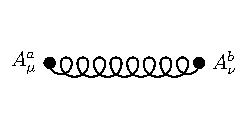
\includegraphics[width=.6\linewidth]{图/Ym-propa.pdf}
    \end{minipage} \begin{minipage}{.45\linewidth}
        \[i\Delta_{\mu\nu}^{ab} =\frac{-i\delta^{ab}}{k^2+i\epsilon}\left(\eta_{\mu\nu} - (1-\xi)\frac{k_\mu k_\nu}{k^2+i\epsilon} \right)\]
    \end{minipage}
    % \vspace{30pt}
\end{center}
\begin{center}
    \begin{minipage}{.5\linewidth}
\centering
%     \begin{fmffile}{YM-3vert}
%   \begin{fmfgraph*}(80,80)
%     \fmfleft{i1,i2}
%     \fmfright{i3}
%     \fmflabel{$A_\mu^a (p)$}{i1}
%     \fmflabel{$A_\nu^b (k)$}{i2}
%     \fmflabel{$A_\lambda^c (q)$}{i3}
%     \fmf{gluon}{i1,v,i2}
%     \fmf{gluon}{i3,v}
%   \end{fmfgraph*}
% \end{fmffile}
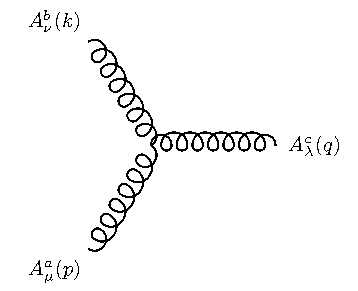
\includegraphics[width=.5\linewidth]{图/YM-3vert.pdf}
\end{minipage}\begin{minipage}{.5\linewidth}
        \[\Gamma_{\mu\nu\lambda}^{abc} = ig f^{abc}\Big( (p-k)_\lambda \eta_{\mu\nu} + (k-q)_\mu\eta_{\nu\lambda} + (q-p)_\nu\eta_{\mu\lambda} \Big)\]
    \end{minipage}
    % \vspace{30pt}
\end{center}
\begin{center}
    \begin{minipage}{.45\linewidth}
    \centering
%         \begin{fmffile}{Ym-4vert}
%   \begin{fmfgraph*}(70,70)
%     \fmfleft{i1,i2}
%     \fmfright{i3,i4}
%     \fmflabel{$A_\mu^a$}{i1}
%     \fmflabel{$A_\nu^b$}{i2}
%     \fmflabel{$A_\lambda^c$}{i3}
%     \fmflabel{$A_\rho^d$}{i4}
%     \fmf{gluon}{i1,v,i2}
%     \fmf{gluon}{i3,v,i4}
%   \end{fmfgraph*}
% \end{fmffile}
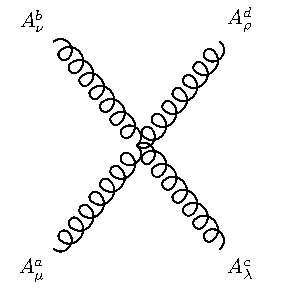
\includegraphics[width=.5\linewidth]{图/YM-4vert.pdf}
    \end{minipage}\begin{minipage}{.45\linewidth}
        \[\begin{split}
\Gamma^{abcd}_{\mu\nu\lambda\rho} = &-ig^2 \Big(f^{abe}f^{cde}(\eta_{\mu\lambda}\eta_{\nu\rho} - \eta_{\nu\lambda}\eta_{\mu\rho})\\ &+ f^{cbe}f^{ade}(\eta_{\mu\lambda}\eta_{\nu\rho}-\eta_{\mu\nu}\eta_{\lambda\rho})\\&+f^{dbe}f^{cae}(\eta_{\mu\nu}\eta_{\lambda\rho}-\eta_{\nu\lambda}\eta_{\mu\rho}) \Big)
        \end{split}\]
    \end{minipage}
        % \vspace{30pt}
\end{center}
\begin{center}
\centering
    \begin{minipage}{.45\linewidth}
    \centering
%         \begin{fmffile}{ghost-propa}
%   \begin{fmfgraph*}(120,20)
%     \fmfipair{i,o}
%     \fmfiequ{i}{(0.2w,0.5h)}
%     \fmfiequ{o}{(0.8w,0.5h)}
%     \fmfiv{d.sh=circle,d.f=1,d.si=2pt,l=$c^a$,l.a=180}{i}
%     \fmfiv{d.sh=circle,d.f=1,d.si=2pt,l=$c^b$,l.a=0}{o}
%     \fmfi{ghost,l.s=left}{i--o}
%   \end{fmfgraph*}
% \end{fmffile}
\vspace{10pt}
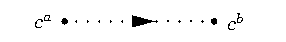
\includegraphics[width=.5\linewidth]{图/ghost-propa.pdf}
\vspace{10pt}
    \end{minipage} \begin{minipage}{.45\linewidth}
        \[i\Delta^{ab} =\frac{-i\delta^{ab}}{k^2+i\epsilon}\]
    \end{minipage}
    % \vspace{30pt}
\end{center}
\begin{center}
    \begin{minipage}{.45\linewidth}
\centering
%     \begin{fmffile}{ghost-YM-int}
%   \begin{fmfgraph*}(80,80)
%     \fmfleft{i1,i2}
%     \fmfright{i3}
%     \fmflabel{$c^a (p)$}{i1}
%     \fmflabel{$c^b (q)$}{i2}
%     \fmflabel{$A_\lambda^c (k)$}{i3}
%     \fmf{ghost}{i1,v,i2}
%     \fmf{gluon}{v,i3}
%   \end{fmfgraph*}
% \end{fmffile}
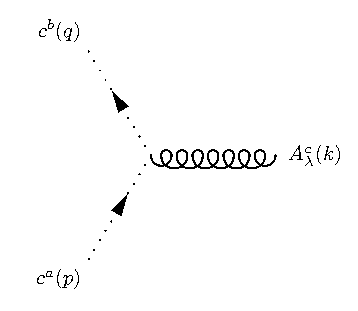
\includegraphics[width=.6\linewidth]{图/YM-ghost.pdf}
\end{minipage}\begin{minipage}{.45\linewidth}
        \[\Gamma_{\mu}^{abc} = -i\frac{g}{2} f^{abc} (k-p-q)_\mu \]
    \end{minipage}
    % \vspace{30pt}
\end{center}

\section{BRST(Becchi-Rouet-Stora-Tyutin)对称性}
现在考虑纯规范场的Lagrangian在洛伦兹规范下可表示为：
\begin{equation}
\mathscr{L}_\text{FP}=-\frac{1}{4}F^a_{\mu\nu}{F^a}^{\mu\nu}-\frac{\lambda}{2}(\partial^\mu A_\mu^a)^2+\partial^\mu\bar{c}^aD_\mu  c^a
\end{equation}
考虑对各场作如下变换：
\begin{equation}
\begin{split}
A^a_\mu&\rightarrow A^a_\mu+\epsilon D_\mu c^a\\
\bar{c}^a&\rightarrow\bar{c}^a-\epsilon \lambda\partial^\mu A_\mu^a\\
c^a&\rightarrow c^a+\epsilon 
\frac{g}{2} f^{abc} c^b c^c
\end{split}\label{eq:brsttrans}
\end{equation}
其中$\epsilon$为满足Grassmann代数的无穷小常量，和鬼场有反对易关系：
\begin{equation}
\{\epsilon,c\}=0,\qquad\{\epsilon,\bar{c}\}=0,\qquad[\epsilon,A_\mu^a]=0
\end{equation}
% 而$\tau$和$\rho$为待定常系数。
将变换带入Lagrangian，得到额外的项
\begin{equation}
    \delta\mathscr{L} = -\lambda\epsilon\partial^\mu D_\mu c^a\partial^\nu A^a_\nu -\lambda \epsilon\partial_\mu\partial^\nu A^a_\nu  D^\mu c^a + \frac{g}{2} \partial_\mu \bar{c}^a D^\mu( \epsilon f^{abc} c^b c^c)
\end{equation}
对第二项进行分部积分，可以将第一项抵消掉，得
\begin{equation}
    \delta\mathscr{L} =-\lambda\epsilon\partial_\mu(\partial^\nu A_\nu ^a D^\mu c^a) + \frac{g}{2} \partial_\mu \bar{c}^a D^\mu( \epsilon f^{abc} c^b c^c)
\end{equation}
对于最后一项，我们有
\begin{equation}
    \frac{g}{2}D^\mu( \epsilon f^{abc} c^b c^c) = -\frac{g^2}{2}(f^{acb}f^{bpq}-f^{apb}f^{bcq}-f^{aqb}f^{bpc})c^c c^p {A^\mu}^q \epsilon=0 
\end{equation}
因此Lagrangian只变化了一个全微分项
\begin{equation}
    \delta\mathscr{L} =-\lambda\epsilon\partial_\mu(\partial^\nu A_\nu ^a D^\mu c^a) = \epsilon\partial_\mu \Lambda^\mu,~~\Lambda^\mu = -\lambda\partial^\nu A^a_\nu D^\mu c^a\label{eq:brsttotd}
\end{equation}
则运动方程保持不变，则变换\eqref{eq:brsttrans}式即为BRST变换。

根据Nöther定理，我们可以通过下式计算守恒流
\begin{equation}
    J^\mu(\epsilon) = -\left( \frac{\partial \mathscr{L}_\text{FP}}{\partial(\partial_\mu A_\nu^a)}\delta A^a_\nu +\delta\bar{c}^a \frac{\partial \mathscr{L}_\text{FP}}{\partial(\partial_\mu\bar{c}^a)} + \frac{\partial \mathscr{L}_\text{FP}}{\partial (\partial_\mu c^a)}\delta c^a \right) + \epsilon \Lambda^\mu
\end{equation}
带入\eqref{eq:brsttrans}，\eqref{eq:brsttotd}式，可得
\begin{equation}
    J^\mu(\epsilon) =\epsilon J^\mu_\text{BRST} = \epsilon\left( -{F^{\mu\nu}}^aD_\nu c^a + \lambda\partial^\nu A_\nu^a D^\mu c^a + \frac{g}{2}f^{abc}\partial^\mu \bar{c}^a c^b c^c \right)
\end{equation}
最终我们可以得到BRST守恒荷
\begin{equation}
    Q_\text{BRST} = \int \mathrm{d}^3\boldsymbol{x} \left( -F^a_{0\nu}D^\nu c^a + \lambda\partial^\mu A_\mu ^a D_0 c^a + \frac{g}{2}f^{abc} \partial_0 \bar{c}^a c^b c^c\right)
    \end{equation}

    考虑我们存在杨-Mills场与Fermion场存在相互作用
    \begin{equation}
        \mathscr{L}=i\psi\slashed{D}\psi-m\bar{\psi}\psi-\frac{1}{4}F^a_{\mu\nu}{F^a}^{\mu\nu}-\frac{\lambda}{2}(\partial^\mu A_\mu^a)^2+\partial^\mu\bar{c}^aD_\mu  c^a
    \end{equation}
此时我们的BRST变换即为
\begin{equation}
\begin{split}
\delta A^a_\mu&= D_\mu c^a\\
\delta c^a&=-  \frac{g}{2} f^{abc} c^b c^c\\
\delta \bar{c}^a&=- \lambda\partial^\mu A_\mu^a\\
\delta \psi & = ig \,c^a \boldsymbol{T}^a \psi
\end{split}\label{eq:brsttrans_wf}
\end{equation}

\section{杨-Mills场单圈重整化}
对于杨-Mills场及参与规范相互作用的费米子场，其裸有效拉氏量为：
\begin{equation}
\begin{split}
    \mathscr{L}_0 = \bar{\psi}_0(i\slashed{\partial} - m_0-g_0 \slashed{A}^a_0\boldsymbol{T}^a)\psi_0 - \frac{1}{2}(\partial_\mu {A_0}_\nu^a \partial^\mu {{A_0}^a}^\nu-\partial_\mu {A_0}_\nu^a \partial^\nu {{A_0}^a}^\mu)-\frac{1}{2\xi_0}(\partial^\mu {A_0}_\mu^a)^2+\partial^\mu\bar{ c_0}^a\partial_\mu c_0^a \\
    -g'_0f^{abc} \partial_\mu {A_0}_\nu^a {{A_0}^\mu}^b{{A_0}^\nu}^c+\frac{1}{4}{g''_0}^2f^{abc}f^{ade}{A_0}_\mu^b {A_0}_\nu^c {{A_0}^\mu}^d {{A_0}^\nu}^e-g'''_0 f^{abc}(\partial^\mu\Bar{c_0}^a) c_0^b  {A_0}_\mu^c
\end{split}
\end{equation}
而重整化拉氏量即为拉氏量加上抵消项：
\begin{equation}
    \begin{split}
        \mathscr{L}_r =&(1+\delta_\psi)\bar{\psi}i\slashed{\partial}\psi  - m(1+\delta_m)\bar{\psi}\psi -(1+\delta_{g_1})g\mu^\epsilon \bar{\psi}\slashed{A}^a\boldsymbol{T}^a\psi - \frac{1+\delta_A}{2}(\partial_\mu {A}_\nu^a \partial^\mu {{A}^a}^\nu-\partial_\mu {A}_\nu^a \partial^\nu {{A}^a}^\mu)\\&-\frac{1+\delta_\xi}{2\xi}(\partial^\mu {A}_\mu^a)^2+(1+\delta_c)\partial^\mu\bar{ c}^a\partial_\mu c^a-g\mu^\epsilon(1+\delta_{g_2}) f^{abc} \partial_\mu {A}_\nu^a {{A}^\mu}^b{{A}^\nu}^c\\
        &+\frac{1+\delta_{g_3}}{4}{g}^2\mu^{2\epsilon}f^{abc}f^{ade}{A}_\mu^b {A}_\nu^c {{A}^\mu}^d {{A}^\nu}^e-g\mu^\epsilon(1+\delta_{g_4}) f^{abc}(\partial^\mu\Bar{c}^a) c^b  {A}_\mu^c
    \end{split}
\end{equation}
则我们有裸场与重整化场的关系：
\begin{equation}
    \psi_0 = \sqrt{1+\delta_\psi}\psi = \sqrt{Z_\psi}\psi,\quad{A_0}_\mu^a = \sqrt{1+\delta_A}A_\mu^a = \sqrt{Z_A}A_\mu^a,\quad c_0^a = \sqrt{1+\delta_c}c^a = \sqrt{Z_c}c^a
\end{equation}
对于裸耦合常数，裸质量及裸规范参数，我们则有：
\begin{align}
    m_0&= \frac{1+\delta_m}{1+\delta_\psi}m = \frac{Z_m}{Z_\psi}m\\
    g_0& = g\mu^\epsilon\frac{1+\delta_{g_1}}{(1+\delta_\psi)\sqrt{1+\delta_A}} = g\mu^\epsilon \frac{Z_1}{Z_\psi Z_A^{1/2}}\\
    g_0'& = g\mu^\epsilon \frac{1+\delta_{g_2}}{(1+\delta_A)^{3/2}}=g\mu^\epsilon\frac{Z_2}{Z_A^{3/2}}\\
    g_0''& = g\mu^\epsilon \frac{\sqrt{1+\delta_{g_3}}}{(1+\delta_A)^2} =g\mu^\epsilon\frac{Z_3^{1/2}}{Z_A^2}\\
    g_0'''&= g\mu^\epsilon \frac{1+\delta_{g_4}}{\sqrt{1+\delta_A}(1+\delta_c)}= g\mu^\epsilon\frac{Z_4}{Z_A^{1/2}Z_c}\\
    \xi_0& = \frac{1+\delta_A}{1+\delta_\xi}\xi=\frac{Z_A}{Z_\xi}\xi
\end{align}
此时，我们需要求解重整化参数$Z_\psi,~Z_A,~Z_c,~Z_m,~Z_\xi,~Z_{1-4}$，便可以对该理论进行重整化。而由于规范(BRST)对称性，这些裸耦合常数本为同一耦合常数$g_0=g'_0=g''_0=g'''_0$，因此有关系：
\begin{equation}
    Z_g= \frac{Z_1}{Z_\psi Z_A^{1/2}} = \frac{Z_2}{Z_A^{3/2}}=\frac{Z_3^{1/2}}{Z_A^{2}}=\frac{Z_4}{Z^{1/2}_AZ_c}
\end{equation}
此关系满足Slavnov–Taylor 恒等式，则我们并不需要求解所有的重整化参数，只需求解这6个独立的重整化参数$Z_\psi,~Z_A,~Z_c,~Z_m,~Z_\xi,~Z_{g}$。
\subsection{杨-Mills规范玻色子自能}
杨-Mills规范玻色子自能$\Pi^{ab}_{\mu\nu} =$包含了费米子圈，玻色子圈及鬼场圈的贡献：
\begin{center}
     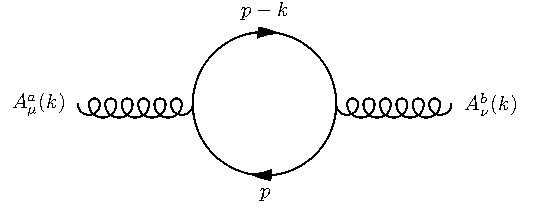
\includegraphics[width=.24\linewidth]{图/ymferloop.pdf}
% \begin{fmffile}{ymfermionloop}
%     \begin{fmfgraph*}(180,60)
%        \fmfleft{i}
%        \fmfright{o}
%        \fmfv{label=$A_\mu^a(k)$,l.a=180}{i}
%        \fmfv{label=$A_\nu^b(k)$,l.a=00}{o}
%        \fmf{gluon,tension=1}{i,v1} 
%        \fmf{gluon,tension=1}{v2,o}
%        \fmf{fermion,left,tension=0.4,label=$p$}{v2,v1}
%        \fmf{fermion,left,tension=0.4,label=$p-k$}{v1,v2}
%     \end{fmfgraph*}
% \end{fmffile}
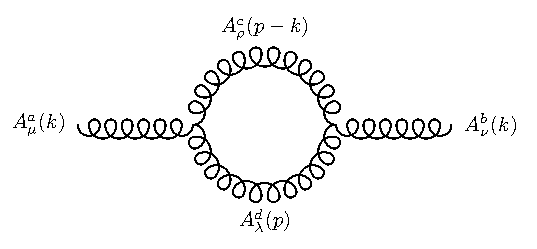
\includegraphics[width=.24\linewidth]{图/ymloop1.pdf}
% \begin{fmffile}{ymloop1}
%     \begin{fmfgraph*}(180,60)
%        \fmfleft{i}
%        \fmfright{o}
%        \fmfv{label=$A_\mu^a(k)$,l.a=180}{i}
%        \fmfv{label=$A_\nu^b(k)$,l.a=00}{o}
%        \fmf{gluon,tension=1}{i,v1} % ,label=H,label.side=left
%        \fmf{gluon,tension=1}{v2,o}
%        \fmf{gluon,left,tension=0.4,label=$A_{\lambda}^d(p)$}{v2,v1}
%        \fmf{gluon,left,tension=0.4,label=$A_{\rho}^c(p-k)$}{v1,v2}
%     \end{fmfgraph*}
% \end{fmffile}
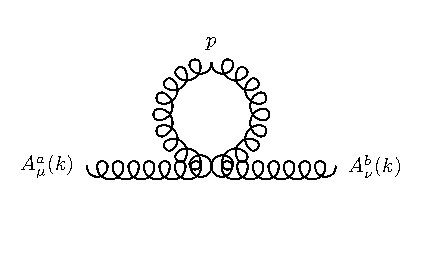
\includegraphics[width=.24\linewidth]{图/ymloop2.pdf}
% \begin{fmffile}{ymloop2}
% \begin{fmfgraph*}(120,100)
%        \fmfleft{i}
%        \fmfright{o}
%        \fmftop{m}
%        \fmfv{label=$A_\mu^a(k)$,l.a=180}{i}
%        \fmfv{label=$A_\nu^b(k)$,l.a=0}{o}
%        \fmflabel{$p$}{m}
%        \fmf{gluon,tension=1}{i,v1}
%        \fmf{gluon,tension=1}{v1,o}
%        \fmf{gluon,left,tension=0}{v1,m,v1}
%     \end{fmfgraph*}
% \end{fmffile}
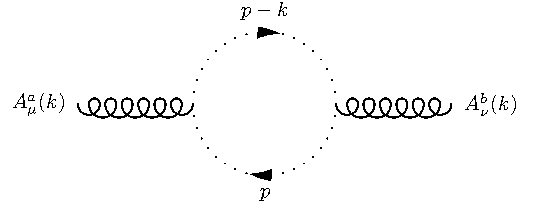
\includegraphics[width=.24\linewidth]{图/ymgholoop.pdf}
% \begin{fmffile}{ymghostloop}
%     \begin{fmfgraph*}(180,60)
%        \fmfleft{i}
%        \fmfright{o}
%        \fmfv{label=$A_\mu^a(k)$,l.a=180}{i}
%        \fmfv{label=$A_\nu^b(k)$,l.a=00}{o}
%        \fmf{gluon,tension=1}{i,v1} % ,label=H,label.side=left
%        \fmf{gluon,tension=1}{v2,o}
%        \fmf{ghost,left,tension=0.4,label=$p$}{v2,v1}
%        \fmf{ghost,left,tension=0.4,label=$p-k$}{v1,v2}
%     \end{fmfgraph*}
% \end{fmffile}
\end{center}
\paragraph{费米子圈}

根据费曼圈积分公示，规范玻色子的费米子圈图即为圈积分：

\begin{figure}[h]
    \centering
    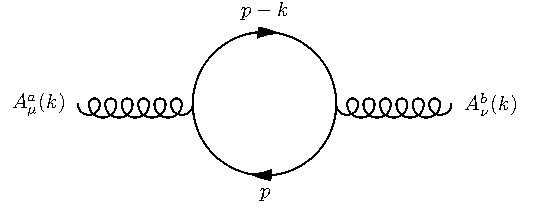
\includegraphics[width=.38\linewidth]{图/ymferloop.pdf}
    \caption{}
    \label{fig:ymferloop}
\end{figure}
\begin{equation}
\begin{split}
\Pi^{ab}_{\mu\nu}(k)&=-\int\frac{\mathrm{d}^{4-\epsilon} p}{(2\pi)^{4-\epsilon}}\operatorname{Tr}\Big[(-ig_0\boldsymbol{T}^a\gamma_\mu)\frac{ i}{\slashed{p}-m}(-ig_0\boldsymbol{T}^b\gamma_\nu)\frac{ i}{\slashed{p}-\slashed{k}-m}\Big]    \\
&=\frac{-i8g^2\mu^{2\epsilon}}{16\pi^2}\operatorname{Tr}(\boldsymbol{T}^a\boldsymbol{T}^b)(k_\mu k_\nu-\eta_{\mu\nu}k^2)\Gamma(\frac{\epsilon}{2})\int_0^1\mathrm{d}x\left(\frac{k^2 x(1-x)+m^2}{4\pi}\right)^{-\frac{\epsilon}{2}}\Big[(x-1)x\Big]
\end{split}
\end{equation}
可以求得：
\begin{equation}
   \Pi^{ab}_{\mu\nu}(k) = \frac{ig^2\delta^{ab}}{16\pi^2}(\eta_{\mu\nu}k^2 - k_\mu k_\nu)\Big[ -\frac{4}{3\epsilon} + 8\int_0^1 (1-x)x\ln\frac{k^2 x(1-x)+m^2}{\mu^2} +\text{finite.}\Big] 
   \label{eq:ymferloop}
\end{equation}


\section{规范对称性自发破缺与BEH机制}
对于杨-Mills场而言，场的质量项$mA_\mu A^\mu$显然破坏了规范对称性，因此杨-Mills场必须为无质量场。然而当我试图描述带质量的规范相互作用时，我们则需要引入额外的机制赋予规范场的质量项。这样的机制假定规范对称性存在于在高能标的情形，此时规范场不具有质量。而当系统自然地过渡到低能标时，规范场的质量项自发的产生，则规范对称性同时自发地被破坏，即称之为“规范对称性自发破缺”。

通常来说场的基态即为真空态，其真空期望值通常为零。然而我们假设拉格朗日中存在某个场，其真空期待值为非零值，那么该场的自由度将会在高于其它场基态的能标中冻结。如果该场还具有不同分量，其分量之间存在着规范对称性，那么如果该场不同分量之间的规范对称性在基态中被破坏的话，便可以在其它场仍能处于自由态的时候，自发的破坏规范对称性。

% 显性的对称性破缺意味着Lagrangian中存在某项，其在对称性变换下无法保持不变。而自发的对称性破缺则是Lagrangian在对称性变换下通常保持不变，但是当系统处于基态时，真空却不是唯一的。如果系统的真空态只有一个，则为对称群中的单态，那么自发对称性破缺则不会发生。而如果真空存在多个简并态，则这些真空态为对称群中的非单态，那么当系统能量最低时，必然只会成为一个物理真空态，此时该物理真空态相对于群中其它的简并真空态而言就是独特的，对称性因此而破缺。

% 我们在研究自然界的基本原理时，往往需要借助对称性来描述一类事物具有的共性。这样的理论虽然十分成功，但是在实际情况中，事物却并不总是表现为具有普遍的共性，而是往往表现为具有普遍的差异性。这就意味着，对称性的破缺现象才是在自然界中普遍存在的。



% 我们以标量场为例：
% \begin{equation}
%     \mathscr{L}=\frac{1}{2}\partial_\mu\phi\partial^\mu\phi-\frac{1}{2}\mu^2\phi^2-\frac{\lambda}{4}\phi^4
% \end{equation}
% 其中场具有内禀对称性$\phi\rightarrow e^{i\alpha}\phi$。此时Lagrangian中的标量势为$V=\frac{1}{2}\mu^2\phi^2+\frac{\lambda}{4}\phi^4$，那么对标量势求一阶导可以找出势能的极小值点，也即真空态：
% \begin{equation}
%     \frac{\partial V}{\partial\phi}=\mu^2\phi+\lambda\phi^3=0
% \end{equation}
% \begin{figure}[H]
%     \centering
% \begin{minipage}{.4\textwidth}
%     \centering
%     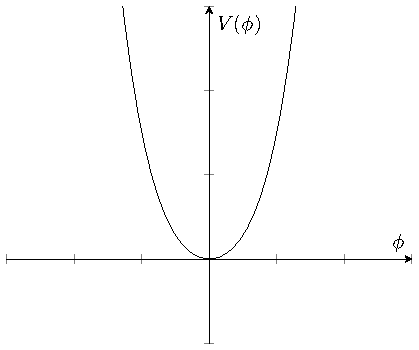
\includegraphics[width=\textwidth]{图/fig_pot_2.pdf}
%     \caption*{$\mu^2>0$}
% \end{minipage}\hfill
% \begin{minipage}{.4\textwidth}
%     \centering
% 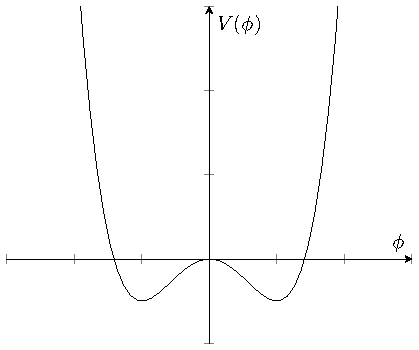
\includegraphics[width=\textwidth]{图/fig_pot_1.pdf}
%  \caption*{$\mu^2<0$}
% \end{minipage}
% \caption{}
% \end{figure}
% 此时当$\mu^2>0$时，标量场$\phi$有且只有一个实根，即标量场的真空期望值$\langle0|\phi|0\rangle=0$，那么真空态即为单态，不发生对称性自发破缺。\\
% 而当$\mu^2<0$时，标量场$\phi$则有非零实根：
% \begin{equation}
%     \langle0|\phi|0\rangle=v=\pm\sqrt{\frac{-\mu^2}{\lambda}}
% \end{equation}
% 此时存在两个简并的真空态，即对应真空期望值$v$为正或负的两个态，但是实际只能有一个物理的真空态。当我们考虑内禀对称性时，可以取参数$\alpha=\pi$，那么对称变换即为$\phi\rightarrow-\phi$，那我们将此对称性带入到真空态时，可得：
% \begin{equation}
%     v=\langle0|\phi|0\rangle\rightarrow \langle0|-\phi|0\rangle=-v
% \end{equation}
% 显然，只要当$v\neq0$时，该对称性在真空态中就不再成立。

% 考虑对称性自发破缺的情况，那么我们定义新的场函数：
% \begin{equation}
%     \phi\rightarrow v+\phi
% \end{equation}
% 带入回Lagrangian中便可得真空态的情形：
% \begin{align}
%     \mathscr{L}&=\frac{1}{2}\partial_\mu\phi\partial^\mu\phi-(\mu^2+\lambda v^2)v\phi-\frac{{\mu^2}+3\lambda v^2}{2}\phi^2-\lambda v\phi^3-\frac{\lambda}{4}\phi^4-\frac{v^2}{2}(\mu^2+\frac{\lambda v^2}{2})\notag\\
%     &=\frac{1}{2}\partial_\mu\phi\partial^\mu\phi-\lambda v^2\phi^2-\lambda v\phi^3-\frac{\lambda}{4}\phi^4+\frac{\lambda}{4}v^4
% \end{align}
% 其中利用了$\mu^2=-\lambda v^2$。此时标量子的质量则为$m=\sqrt{2\lambda}v$，且获得了额外的三相互作用顶点。
我们现在考虑一个复标量场$\phi$，该场具有自相互作用势能$V(\phi)$:
\begin{gather}
    \mathscr{L}=\partial^\mu\phi^\dagger\partial_\mu\phi-V(\phi)\\
    V(\phi)=\mu^2\phi^\dagger\phi+{\lambda}(\phi^\dagger\phi)^2
\end{gather}
同时该场具有SU($N$)规范对称性$\phi(x)\rightarrow e^{i\omega^a(x)\boldsymbol{T}^a}\phi(x)$，其分量为SU($N$)规范对称群的多重态。那么在场处于真空态时，有势能极小值条件：
\begin{equation}
    \frac{\partial V}{\partial\phi}=\Big(\mu^2+2\lambda(\phi^\dagger\phi)\Big)\phi^\dagger=0
\end{equation}
\begin{figure}[h]
    \centering
    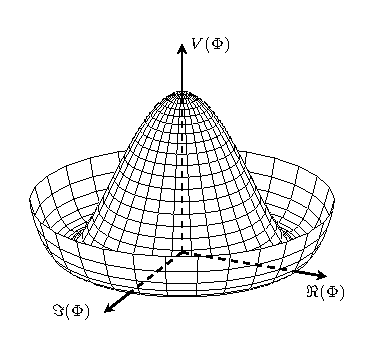
\includegraphics{图/higgspot.pdf}
    \caption{}
    \label{fig:higgspot}
\end{figure}
当$\mu^2>0$时，只有唯一真空态，其真空期望值为$\langle0|\phi|0\rangle=0$。而当$\mu^2<0$时，势能的形状则如图\ref{fig:higgspot}所示，存在非平庸真空期待值：
\begin{equation}
    \langle0|\phi^\dagger\phi|0\rangle=-{\frac{\mu^2}{2\lambda}}=\frac{v^2}{2}
\end{equation}
由于$\phi$为规范群多重态，所以$|\phi|^2=\sum^N_i \phi_i^*\phi_i=\sum^N_i(\Re(\phi_i)^2+\Im(\phi_i)^2)=\frac{v^2}{2}$。此时我们有无限多个简并的真空态，那么我们人为选定其中一个分量$\langle0|\Re(\phi_i)|0\rangle=v/\sqrt{2}$，其它所有分量的真空期待值为0，即：
\begin{equation}
    \langle0|\phi|0\rangle=\begin{pmatrix}
    0\\
    \vdots\\
    \frac{v}{\sqrt{2}}%\\
    %0&  \cdots& v
    \end{pmatrix}
\end{equation}
我们对场的真空态作对称变换：
\begin{align}
    \frac{v_i}{\sqrt{2}}=\langle0|\phi_i|0\rangle\rightarrow&\langle0|e^{i\omega^a\boldsymbol{T}^a}\phi_i|0\rangle=\langle0|(1+{i\omega^a\boldsymbol{T}^a_{ij}})\phi_i|0\rangle\notag\\
    &=\frac{v_i}{\sqrt{2}}+i\omega^a\langle0|\boldsymbol{T}^a_{ij}\phi_i|0\rangle
\end{align}
如果真空态在规范变换下不变，那么我们显然可得只有当$\langle0|\boldsymbol{T}_{ij}^a\phi_i|0\rangle=0$时，规范对称性在真空态中才能保存。然而这条件并不能对所有群生产元$\boldsymbol{T}^a$成立。因此由于非零真空期待值的存在，这些简并态之间本来存在的SU($N$)规范对称性便遭到破坏，即为规范对称性的自发破缺。

然而对于$\langle0|\boldsymbol{T}_{ij}^a\phi_i|0\rangle=0$的情况，实际上意味着在规范群$G$中，存在着不变子群$H\subset G$，使得即使在真空态中规范对称性被破坏时，该子群的元素依然保留着规范对称性。对于这种特殊情况，我们考虑真空态中的势$V(\phi)$，其具有规范对称性：
\begin{equation}
    \langle0|\delta V|0\rangle=\langle0|\frac{\partial V}{\partial \phi_i}\delta\phi_i|0\rangle = i\omega^a \langle0|\frac{\partial V}{\partial \phi_i}\boldsymbol{T}^a_{ij} \phi_j|0\rangle=0
\end{equation}
由于$\omega^a$为任意参数，因此有：
\begin{equation}
    \langle0|\frac{\partial V}{\partial \phi_i}\boldsymbol{T}^a_{ij} \phi_j|0\rangle=0
\end{equation}
然后在对此作一次微商：
\begin{equation}
       \frac{\partial^2 V}{\partial \phi_i\partial\phi_k}\Big|_{\phi = v/\sqrt{2}}\langle0|\boldsymbol{T}^a_{ij} \phi_j|0\rangle+\frac{\partial V}{\partial \phi_i} \Big|_{\phi = v/\sqrt{2}}\boldsymbol{T}^a_{ik}=0
\end{equation}
其中由于$\phi = v/\sqrt{2}$处为势的极小值点，所以有$\frac{\partial V}{\partial \phi_i} \Big|_{\phi = v/\sqrt{2}}=0$，则可得：
\begin{equation}
    \frac{\partial^2 V}{\partial \phi_i\partial\phi_k}\Big|_{\phi = v/\sqrt{2}}\langle0|\boldsymbol{T}^a_{ij} \phi_j|0\rangle=0
    \label{eq:gsth}
\end{equation}
如果我们将势围绕真空态展开，则有：
\begin{equation}
    V(\phi)=V(v) +\frac{1}{2}\frac{\partial^2 V}{\partial \phi_i\partial\phi_k}\Big|_{\phi = v/\sqrt{2}}(\phi_i-\frac{v}{\sqrt{2}})(\phi_k-\frac{v}{\sqrt{2}})+\cdots
\end{equation}
而势的二阶微商则为场的质量项，因此我们可以得到场的质量矩阵：
\begin{equation}
    M^2_{ij}=\frac{\partial^2 V}{\partial \phi_i\partial\phi_k}\Big|_{\phi = v/\sqrt{2}}
\end{equation}
从\eqref{eq:gsth}式中，我们容易看出，当$\langle0|\boldsymbol{T}^a_{ij} \phi_j|0\rangle\neq0$时，必然有$M^2_{ik}=0$。而当$\langle0|\boldsymbol{T}^a_{ij} \phi_j|0\rangle=0$时，则有可能存在非零质量项。综合之前的讨论，对于规范群$G$中的子群$H$以外的部分，其维度为$\mathrm{dim}(G/H)=\mathrm{dim}(G)-\mathrm{dim}(H)$，则总体系中至少存在$\mathrm{dim}(G/H)$个无质量标量场，我们称此场为Goldstone玻色子。%，该结论即为Goldstone定理。
因此，我们可得Goldstone定理：当一个自由度为$n$的连续对称型自发破缺之后，必然会产生$n$个Goldstone玻色子。

现在我们可以在围绕真空期望值的基础上定义无穷小的新场：
\begin{equation}
    \phi(x)=\frac{v+ H(x)}{\sqrt{2}}\exp\left(i\frac{\omega^a(x)\boldsymbol{T}^a}{v}\right)
    \label{eq:phiv}
\end{equation}
其中$H(x)$为实标量场，带入回Lagrangian中，得：
\begin{align}
    \mathscr{L}=&\frac{1}{2}\partial^\mu H\partial_\mu H+\frac{1}{2}\left(1+\frac{H}{v}\right)^2\partial^\mu\omega^a\partial_\mu\omega^a-\frac{1}{2}\mu^2(v+ H)^2-\frac{\lambda}{4}(v+ H)^4%\notag\\
    % \approx&\partial^\mu\rho\partial_\mu\rho+v^2\partial^\mu\omega^a\partial_\mu\omega^a-2\lambda v^2\rho^2-2\lambda v\rho^3-\frac{\lambda}{2}\rho^4+\cdots\notag\\
    % \approx&\partial^\mu\rho\partial_\mu\rho+v^2\partial^\mu\omega^a\partial_\mu\omega^a-2\lambda v^2\rho^2+\text{interactions}
\end{align}
同时将$\lambda=-\mu^2/v^2$带入，得
\begin{equation}
\begin{split}
    \mathscr{L}=&\frac{1}{2}\partial^\mu H\partial_\mu H+\mu^2 H^2  +\frac{\mu^2}{v} H^3+\frac{\mu^2}{4v^2} H^4+\frac{1}{2}\mu^2 v^2\\
    &+ \frac{1}{2} \partial^\mu\omega^a\partial_\mu\omega^a +\frac{H}{v} \partial^\mu\omega^a\partial_\mu\omega^a + \frac{H^2}{2v^2}\partial^\mu\omega^a\partial_\mu\omega^a
\end{split}
\end{equation}
可以看到，只有$ H$场获得了质量$m^2=-2\mu^2$，而所有其它的$\omega^a$场都为无质量的玻色子场。我们可得：
\begin{equation}
\begin{split}
    \mathscr{L}=&\frac{1}{2}\partial^\mu H\partial_\mu H-\frac{1}{2}m^2 H^2  -\frac{m^2}{2v} H^3-\frac{m^2}{8v^2} H^4-\frac{1}{4}m^2 v^2\\
    &+ \frac{1}{2} \partial^\mu\omega^a\partial_\mu\omega^a +\frac{H}{v} \partial^\mu\omega^a\partial_\mu\omega^a + \frac{1}{2v^2}H^2\partial^\mu\omega^a\partial_\mu\omega^a
\end{split}
\end{equation}

当我们考虑该场参与规范相互作用时，则有：
\begin{equation}
    \mathscr{L}=(D^\mu\phi)^\dagger D_\mu\phi-V(\phi),\qquad D_\mu = \partial_\mu -igQ A_\mu%^a \boldsymbol{T}^a
\end{equation}
我们得：
\begin{equation}
    \mathscr{L}=\partial^\mu\phi^\dagger\partial_\mu\phi+g^2Q^2A_\mu A^\mu \phi^\dagger\phi + igQA_\mu(\phi^\dagger\partial^\mu \phi - \partial^\mu\phi^\dagger \phi)-V(\phi)
\end{equation}
同理，我们带入真空态附近的场函数\eqref{eq:phiv}，我们可得：
\begin{equation}
\begin{split}
    \mathscr{L}=&\frac{1}{2}\partial^\mu H\partial_\mu H-\frac{1}{2}m^2 H^2  -\frac{m^2}{2v} H^3-\frac{m^2}{8v^2} H^4-\frac{1}{4}m^2 v^2\\
    &+  \frac{g^2Q^2v^2}{2}A_\mu A^\mu + g^2Q^2 v A_\mu A^\mu  H + \frac{g^2Q^2}{2}  H^2 A_\mu A^\mu\\
    &+ \left(1+\frac{H}{v}\right)^2\frac{1}{2}\partial^\mu\omega \partial_\mu\omega  -g v A_\mu \partial^\mu\omega \left(1+\frac{H}{v}\right)^2
\end{split}
\end{equation}
则规范场$A_\mu$获得了质量项$m_A^2=g^2 Q^2 v^2$，Lagrangian可以写为：
\begin{equation}
\begin{split}
    \mathscr{L}=&\frac{1}{2}\partial^\mu H\partial_\mu H-\frac{1}{2}m^2 H^2  -\frac{m^2}{2v} H^3-\frac{m^2}{8v^2} H^4-\frac{1}{4}m^2 v^2\\
    &+ \frac{1}{2}\partial^\mu\omega \partial_\mu\omega  +\frac{H}{v} \partial^\mu\omega \partial_\mu\omega  + \frac{1}{2v^2}H^2\partial^\mu\omega \partial_\mu\omega \\
    &+ \frac{1}{2}m_A^2 A_\mu A^\mu + \frac{m_A^2}{v} A_\mu A^\mu  H +\frac{m_A^2}{2v^2} H^2 A_\mu A^\mu\\
    &-m_A A_\mu \partial^\mu\omega - 2\frac{m_A}{v} H A_\mu\partial^\mu\omega - \frac{m_A}{v^2} H^2 A_\mu\partial^\mu\omega
\end{split}
\end{equation}
其中$-m_A A_\mu \partial^\mu\omega$项会带来$A_\mu$场和$\omega$场的混合，而由于$A_\mu$场的规范对称性，我们可以引入一个规范场的规范变换来消除掉该项，称之为幺正规范。此时新的规范场为：
\begin{equation}
    A_\mu \rightarrow e^{\frac{-i\omega(x)}{v}}A_\mu e^{\frac{i\omega(x)}{v}} - \frac{1}{m_A}\partial_\mu \omega(x)
\end{equation}
此时，我们可得：
\begin{equation}
    D_\mu \phi = \frac{1}{\sqrt{2}}e^{\frac{-i\omega(x)}{v}}(\partial_\mu H -igA'_\mu (v+H))
\end{equation}
则Lagrangian为：
\begin{equation}
\begin{split}
    \mathscr{L}=&\frac{1}{2}\partial^\mu H\partial_\mu H-\frac{1}{2}m^2 H^2  -\frac{m^2}{2v} H^3-\frac{m^2}{8v^2} H^4-\frac{1}{4}m^2 v^2\\
    &+ \frac{1}{2}m_A^2 A_\mu {A}^\mu + \frac{m_A^2}{v} A_\mu {A}^\mu  H +\frac{m_A^2}{2v^2} H^2 A_\mu {A}^\mu
\end{split}
\end{equation}

因此，我们可以看出，规范场$A_\mu$通过这样的规范对称性破缺机制获得了质量项，并同时将无质量的Goldestone玻色子场$\omega$“吃掉”，这样的机制即为Brout-Englert-Higgs机制，而标量场$\phi$即为Higgs场，产生的标量粒子即为Higgs玻色子。
% \section{基本粒子标准模型}

% 标准粒子物理模型包含了组成物质的费米子以及传递相互作用的规范玻色子，其中胶子作为SU(3)$_\text{C}$规范群的生成元传递了夸克间的强相互作用，而$W/Z$玻色子作为SU(2)$_\text{L}$群生成元传递弱相互作用。
而对于规范群中的费米子而言，我们考虑中其与Higgs场的相互作用：%在Weyl表象
\begin{equation}
    \mathscr{L}=i\bar{\psi}\slashed{D}\psi  - (Y_\text{f} \bar{\psi}_L \phi \psi_R+\mathrm{h.c.}) - V(\phi)
    \label{eq:Higgsfermions}
\end{equation}
其中$Y_f$称之为汤川耦合，即为汤川相互作用。当费米子和Higgs场都为规范SU(2)群的多重态时，Higgs场具有4个分量，因此Higgs势$V(\phi)$具有整体SO(4)对称性。由于SO(4)对称性同构于两个独立的SU(2)对称性，因此方程\eqref{eq:Higgsfermions}中的Lagrangian具有整体的SO(4)$=$SU($N)_L\otimes$SU($N)_R$对称性，即Lagrangian在以下变换中
\begin{gather}
    \phi\rightarrow e^{i\alpha_L^a\boldsymbol{T}^a }\phi~ e^{-i\alpha_R^a\boldsymbol{T}^a }\\
    \psi_L \rightarrow e^{i\alpha_L^a\boldsymbol{T}^a }\psi_L\\
    \psi_R \rightarrow e^{i\alpha_R^a\boldsymbol{T}^a }\psi_R
\end{gather}
保持不变。其中在Weyl表象中分别对应了左手费米子$\psi_L$的整体SU(2)$_L$对称性和右手费米子$\psi_R$的整体SU(2)$_R$对称性。
但是当规范对称性破缺时，该整体对称性也会发生破缺，此时Higgs势的整体对称性破缺为SO(3)对称性，同构于SU(2)对称性。在Weyl表象中则表为
\begin{equation}
    \mathrm{SU(2)}_L\otimes\mathrm{SU(2)}_R\rightarrow \mathrm{SU(2)}_V
\end{equation}
即费米子在发生规范对称性自发破缺以后，依然保留了SU(2)$_V$对称性，称之为看守对称性。

总而言之，我们可以将规范群中的费米子场和Higgs场，以及规范玻色子场综合起来，得到如下Lagrangian：
\begin{equation}
    \mathscr{L}=(D^\mu \phi)^\dagger (D_\mu \phi) + i\bar{\psi}\slashed{D}\,\psi -\frac{1}{4}{F^a}_{\mu\nu}{F^a}^{\mu\nu}  - (Y_\text{f} \,\bar{\psi}_L \phi\, \psi_R+\mathrm{h.c.}) - V(\phi)
    \label{eq:smlagrangian}
\end{equation}
即为粒子物理标准模型Lagrangian。

\epigraphhead[650]{}
\part{拓展理论}
\chapter{有效场论}
在物理学理论的发展过程中，人们对于物理学的理解是一个逐步认知的过程。比如，经典力学理论只能描述宏观尺度，且速度较低的运动。而当人们接触到接近光速的情形时，便发展出了相对论理论。同时当我们回过头研究低速情形时，可以对相对论的速度$\beta$做高阶展开$E=mc^2/\sqrt{1-\beta^2}\approx mc^2 + \frac{1}{2}mc^2 \beta^2+\mathcal{O}(\beta^4)+\cdots$。其中第二项则回归到经典力学情形$E=\frac{1}{2}mv^2$，同时增加了静止质量项$mc^2$。而当人们开始研究低速运动的微观粒子的规律，则构建了量子力学。同样对于量子力学中的路径积分$Z = e^{\frac{i}{\hbar}\mathcal{S}}$，我们可以对在宏观尺度下极小的普朗克常数$\hbar$做高阶展开$Z = \exp{\frac{i}{\hbar}(\mathcal{S}^{(0)} - i\hbar \mathcal{S}^{(1)} + \mathcal{O}((i\hbar)^2)+\cdots}$，即为WKB半经典近似，便可回归到经典的Hamliton-Jacobi方程。

% 从以上例子中我们发现，虽然物理理论会发展到更高尺度下更加普适的理论，但是对于某个特定尺度，更加的普适的理论反而更加难以计算结果。而我们对普适理论中的尺度参数做高阶展开后，其中的前几项便是该尺度下的有效理论。通常我们将这种通过对普适理论做高阶展开得到有效理论的方法，称之为``Top-down''。相反，如果我们实验数据发现，我们的目前使用的理论存在某些修正项，那么意味着这些修正项将会把我们指引到更高尺度的普适理论，这样的过程称之为``Bottom-up''。

% \begin{equation}
%     \mathscr{L} = \sum_n \epsilon^n \mathscr{L}^{(n)}= \mathscr{L}^{(0)} + \epsilon\mathscr{L}^{(1)} + \mathcal{O}(\epsilon^2)+\cdots
% \end{equation}

在量子场论中，实际上圈图的重整化预示着量子场论只能描述特定能标$\Lambda$下的物理，这恰好符合了有效理论的描述。而我们将量子场截断到某个能标下的表述形式便是有效场论。则我们可以将拉氏量对参数$\frac{1}{\Lambda}$做高阶展开：
\begin{equation}
    \mathscr{L}_\mathrm{eff} =\mathscr{L}_0^{(d=4)}+\frac{\mathcal{C}_1}{\Lambda} \mathscr{L}^{(d=5)}+\frac{\mathcal{C}_2}{\Lambda^2} \mathscr{L}^{(d=6)}+\mathcal{O}(\frac{1}{\Lambda^3})+\cdots
\end{equation}
% \section{有效拉格朗日量}
% \section{级次展开与Wilson系数}
% %\section{重整化群优化微扰论}
% \section{线性$\sigma$模型}
\section{重场展开}

我们考虑一个与外源相互作用的系统，考虑其作用量包含了较重背景场$\Phi$以及较轻外源场$\varphi$的动能项和相互作用项，则有
\begin{equation}
    \mathcal{S}[\Phi,\varphi] = \int\mathrm{d}x\, \Big(\Phi_i\Delta^{-1}(\Phi)_{ij} \Phi_j + g J(\varphi)_k\Phi_k  + \varphi_l D^{-1}(\varphi)_{lm}\varphi_m\Big)
\end{equation}
其连通Green函数生成泛函可表为（\eqref{eq:congreen}式）
\begin{equation}
    W[J] = \ln \mathscr{Z}[J] =  -{g^2}\int\mathrm{d}{x}\mathrm{d}{x}'\,  J^*(x) \Delta(x-x')J(x') = -{g^2}\int\mathrm{d}x\int{\mathrm{d}q}\, J^*(p) \Delta(p-q)\delta(p-q) J(q)
\end{equation}
则有效作用可以表示为
\begin{equation}
\begin{split}
        \Gamma[\varphi]&= -i\ln\mathscr{Z}[J(\varphi)]-g\int\mathrm{d}x\, J(\varphi)\Phi = \int\mathrm{d}x \,\Big[ -{g^2}J_i^*(\varphi) \frac{k_{ij}}{p^2 - M^2+i\epsilon} J_j(\varphi) -gJ(\varphi)\Phi  \Big]\\
        &= \int\mathrm{d}x\Big[ \varphi_l D^{-1}_{lm}\varphi_m  -{g^2}J_i^*(\varphi) \frac{k_{ij}}{p^2 - M^2+i\epsilon} J_j(\varphi)\Big]
\end{split}
\end{equation}
其中有效作用量的$J(\varphi)\Phi$的相互作用项可以用轻场的运动方程替换，则变为轻场的动能项。
此时重场表现为几乎静止，那么其质量项必然远远大于其动量$M^2\gg p^2$，则我们可以对重场的传播子$\Delta$围绕$\frac{p^2}{M^2}\sim0$作展开，得
\begin{equation}
\begin{split}
    \Gamma[\varphi] =& \int\mathrm{d}x \Big[\varphi_l D^{-1}_{lm}\varphi_m - g^2 J_i^*(\varphi)\frac{k_{ij}}{M^2}\left(\frac{1}{\frac{p^2}{M^2}-1} \right)J_j(\varphi)\Big] \\\approx&  \int\mathrm{d}x \Big[\varphi_l D^{-1}_{lm}\varphi_m + g^2 J_i^*(\varphi)\frac{k_{ij}}{M^2}\left(1 + \frac{p^2}{M^2} +\mathcal{O}\left( \frac{p^4}{M^4} \right)+\cdots \right)J_j(\varphi)\Big]\\
    \approx&\int\mathrm{d}x\Big[\varphi_l D^{-1}_{lm}\varphi_m +  \frac{g^2}{M^2}J^*_i(\varphi)  J_i(\varphi) \Big]
\end{split}
\end{equation}
则此时整个体系的作用量只保留轻场的动能项和运动，重场的自由度被忽略不计，而轻场与重场的之间参与相互作用表现形式则变为了两个轻场流之间直接相互作用，重场的自由度则贡献到了相互作用常数中
\begin{equation}
    \mathscr{L}_\mathrm{eff} (\varphi) = \varphi_l D^{-1}_{lm}\varphi_m +  GJ^*_i(\varphi)  J_i(\varphi),~~~~G = \frac{g^2}{M^2}\sim\frac{1}{\Lambda^2}
\end{equation}
最终，新的相互作用耦合常数$G$不再是无量纲常数，而是依赖于重场质量，且量纲为-2的耦合常数。而对于轻场相互作用项$J^*_i(\varphi)  J_i(\varphi)$，其量纲为6，大于可重整化的要求$d\leq4$，因此该项只能被算作有效算符，该理论只能在能标远低于重场质量的情形下适用，而不能作为完备的全能标普适理论。而此时如果实验上发现了$[G]\geq 2$的有效理论，则意味着该理论有可能存在一个更重的未被发现的场，贡献到了相互作用耦合常数上。

如果我们考虑轻场是费米子场，而重场是$W$玻色子场，则费米子与$W$相互作用的弱相互作用理论在低能标下可以转变为有效的四费米子理论
\begin{equation}
    \mathscr{L}_\mathrm{eff} \approx i\bar{\psi}(\partial\!\!\!/-m)\psi + \frac{G_F}{\sqrt{2}}(\bar{\psi}_R\gamma^\mu\psi_L)(\bar{\psi}_L\gamma_\mu\psi_R) + \mathrm{h.c.},~~~~\frac{G_F}{\sqrt{2}} = \frac{g_2^2}{8M_W^2}
\end{equation}

\section{单圈有效势能}

对于场$\phi$，我们可以考虑将场分解为静止的经典背景场$\phi_0$和较小的涨落场$\varphi$，即$\phi=\phi_0+\varphi$。那么我们可以对作用量围绕$\phi_0$进行展开
\begin{equation}
    % \mathscr{V}(\phi_0 + \varphi) = \mathscr{V}(\phi_0) + \mathscr{V}'(\phi_0)\,\varphi + \frac{1}{2!} \mathscr{V}''(\phi_0)\,\varphi^2 + \frac{1}{3!}\mathscr{V}'''(\phi_0)\,\varphi^3 + \frac{1}{4!} \mathscr{V}''''(\phi_0)\,\varphi^4 + \dots
    S[\phi_0 + \varphi] = S[\phi_0] + \int \mathrm{d}^4x \, \frac{\delta S}{\delta \phi(x)}\bigg|_{\phi_0} \varphi(x) + \frac{1}{2} \int \mathrm{d}^4x \mathrm{d}^4y \, \varphi(x) \frac{\delta^2 S}{\delta \phi(x)\delta \phi(y)}\bigg|_{\phi_0} \varphi(y) + \mathcal{O}(\varphi^3)+  \cdots
\end{equation}
其中不考虑外源的情况下，第一项展开式可以用运动方程$\frac{\delta\mathcal{S}}{\delta \phi}=0$代替，同时我们可以略去$\mathcal{O}(\varphi^3)$等更高阶小量，因此只保留两项。
当我们考虑路径积分时，我们则可以将小场$\varphi$贡献积分掉，即
\begin{equation}
\begin{split}
    \mathcal{Z} &= \int\mathcal{D}\phi_0\, e^{-\mathcal{S}[\phi_0]}\int\mathcal{D}\varphi\, \exp\Big( \frac{1}{2}\int \mathrm{d}^4x\frac{\delta^2\mathcal{S}}{\delta\phi(x)^2}\Big|_{\phi_0}\varphi(x)^2  \Big)\\
    &=\mathcal{Z}_0 \Big(\operatorname{det} \Big[\int \mathrm{d}^4x\frac{\delta^2\mathcal{S}}{\delta\phi(x)^2}\Big|_{\phi_0} \Big] \Big)^{-1/2}
    % =\mathcal{Z}_0 \Big(\operatorname{det} \Big[\int \mathrm{d}^4x(-\partial_\mu\partial^\mu - \mathscr{V}''(\phi_0))\Big] \Big)^{-1/2}
\end{split}
\end{equation}
因此有效作用量可以表示为
\begin{equation}
    \Gamma[\phi_0] = -\ln\mathcal{Z} = \mathcal{S}[\phi_0] + \frac{1}{2}\int \mathrm{d}^4x\,\operatorname{tr}\ln \left( \frac{\delta^2\mathcal{S}}{\delta\phi(x)^2}\Big|_{\phi_0}  \right)+\cdots
\end{equation}
其中有效作用量的第二项为理论的单圈修正项，而其中的求迹则是对四动量空间的求和。由于$\phi_0$场为几乎静止的背景场，其动能项几乎可以忽略不计，则$\mathcal{S}[\phi_0]$中只包含势能项，则我们可以根据\eqref{eq:veff0}式中的有效势能定义，可得有效势能为
\begin{equation}
    \mathscr{V}_\mathrm{eff}(\phi_0) = \mathscr{V}(\phi_0) - \frac{1}{2}\operatorname{tr}\ln\left( \frac{\delta^2\mathcal{S}}{\delta\phi(x)^2}\Big|_{\phi_0}  \right)+\cdots
\end{equation}

如果我们具体考虑带势能项的标量场
\begin{equation}
    \mathcal{S}[\phi] = \int \mathrm{d}^4x \Big[\frac{1}{2} (\partial_\mu \phi)(\partial^\mu \phi) - \mathscr{V}(\phi)\Big]
\end{equation}
那么可得展开式
% \begin{equation}
%     \begin{split}
%         \mathcal{S}[\phi_0,\varphi] = \int \mathrm{d}^4x \Big[& \frac{1}{2}(\partial_\mu \phi_0)^2 - \mathscr{V}(\phi_0)
%         -[\partial_\mu\partial^\mu\phi_0 +\mathscr{V}'(\phi_0)]\varphi
%         -\frac{1}{2}[\partial_\mu\partial^\mu + \mathscr{V}''(\phi_0)]\varphi^2\\
%         &-\frac{1}{3!}\mathscr{V}'''(\phi_0)\,\varphi^3 - \frac{1}{4!} \mathscr{V}''''(\phi_0)\,\varphi^4 - \dots\Big]
%     \end{split}
% \end{equation}
\begin{equation}
\begin{split}
        \mathcal{S}[\phi_0,\varphi]  = \int \mathrm{d}^4x \Big[ \frac{1}{2}(\partial_\mu \phi_0)^2- \mathscr{V}(\phi_0)+\frac{1}{2}(\partial_\mu \varphi)^2-\frac{1}{2}\mathscr{V}''(\phi_0)\varphi^2 - \dots\Big]
\end{split}
\end{equation}
那么有效作用量可以表示为
\begin{equation}
\begin{split}
       \Gamma[\phi_0] =& \int\mathrm{d}^4x \Big[ \frac{1}{2}(\partial_\mu \phi_0)^2- \mathscr{V}(\phi_0) +\frac{1}{2}\operatorname{tr}\ln\left( -\partial^2 -\mathscr{V}''(\phi_0) \right)+\cdots\Big] \\
       =&\int\mathrm{d}^4x \Big[ \frac{1}{2}(\partial_\mu \phi_0)^2- \mathscr{V}(\phi_0) +\frac{1}{2}\int\frac{\mathrm{d}^4p}{(2\pi)^4}\ln\left( p^2 -\mathscr{V}''(\phi_0) \right)+\cdots\Big]
\end{split}
\end{equation}
其中将求迹转化为对动量空间的积分。带入$\phi^4$理论，即$\mathscr{V}(\phi)  = \frac{1}{2}m^2\phi^2 + \frac{\lambda}{4!}\phi^4$可得
\begin{equation}
    \begin{split}
        \mathcal{S}[\phi_0,\varphi] = \int \mathrm{d}^4x \Big[&\frac{1}{2}(\partial_\mu \phi_0)^2-\frac{1}{2}m^2\phi_0^2-\frac{\lambda}{4!}\phi_0^4\\
        &+\frac{1}{2}(\partial_\mu \varphi)^2-\frac{1}{2}\Big(m^2+\frac{\lambda}{2}\phi_0^2\Big)\varphi^2 -\frac{\lambda}{6}\phi_0\varphi^3 - \frac{\lambda}{4!}\varphi^4\Big]
    \end{split}
\end{equation}
仅保留$\varphi^2$项，即首阶修正项，则可得有效作用量为
\begin{equation}
    \Gamma[\phi_0] = \int\mathrm{d}^4x \Big[ \frac{1}{2}(\partial_\mu \phi_0)^2- \frac{1}{2}m^2\phi_0^2 -\frac{\lambda}{4!}\phi_0^4 +\frac{1}{2}\int\frac{\mathrm{d}^4p}{(2\pi)^4}\ln\left( p^2 -m^2-\frac{\lambda}{2}\phi_0^2 \right)+\cdots\Big]
\end{equation}
由于$\phi_0$场为几乎静止的背景场，其动能项几乎可以忽略不计$\frac{1}{2}(\partial_\mu\phi_0)^2\approx 0$，则我们由此可得有效势能
\begin{align}
\mathscr{V}_\mathrm{eff}(\phi_0) &= \mathscr{V}(\phi_0) - \frac{1}{2}\int\frac{\mathrm{d}^4p}{(2\pi)^4}\ln\left( p^2 -\mathscr{V}''(\phi_0) \right)+\cdots \\
    \mathscr{V}_\mathrm{eff}(\phi_0) &= \frac{1}{2}m^2\phi_0^2 +\frac{\lambda}{4!}\phi_0^4 - \frac{1}{2}\int\frac{\mathrm{d}^4p}{(2\pi)^4}\ln\left( p^2 -m^2-\frac{\lambda}{2}\phi_0^2 \right)+\cdots
\end{align}

\chapter{有限温度场论}
在之前的讨论中，我们通常考虑的物理过程是瞬时的相互作用过程。然而，当我们考虑整个系统经历了足够长时间的内部相互作用后，达到了平衡态，那么此时系统的时间依赖性则会被积分掉，从而转化为系统的温度参数。我们考虑经历了足够长的时间$\beta$后达到热平衡态，则系统的温度为$T=\frac{1}{\beta}$。我们可以看出当系统经历的是瞬时过程，即$\beta\rightarrow0$，则温度$T\rightarrow\infty$趋于无穷大。而当时间足够长时，温度则为有限值，这种情形下的量子场论理论即为有限温度量子场论。也叫热量子场论。

考虑系统的路径积分$\mathcal{Z}=\int \mathcal{D}\phi\,\exp(i\int\mathrm{d}t\,\mathcal{L})$中的时间积分，根据柯西定理，我们有
\begin{equation}
    \int_{0}^{\infty} \mathrm{d}t ~\mathcal{L} + \int_{i\infty}^0\mathrm{d}t ~\mathcal{L} = 0
\end{equation}
对于虚轴上的积分，我们可以将时间参数$t$转化为虚时间$t=-i\tau$，即通过Wick转动将对时间$t$的积分转化为虚时间$\tau$的积分：
\begin{equation}
    i\int_{0}^{\infty} \mathrm{d}t ~\mathcal{L} = - \int_{i\infty}^0 i\mathrm{d}t ~\mathcal{L} =  \int_{\infty}^0\mathrm{d}\tau ~\mathcal{L}(-i\tau) = \int_0^\infty \mathrm{d}\tau ~ [-\mathcal{L}(-i\tau)]
\end{equation}
而此时对于时空度规，我们则有：
\begin{equation}
    \mathrm{d}s^2 = \mathrm{d}t^2 - \mathrm{d}\boldsymbol{x}^2 = -(\mathrm{d}\tau^2 + \mathrm{d}\boldsymbol{x}^2)
\end{equation}
此时在$x_\mu=(\tau,\boldsymbol{x})$的坐标系中，时空度规变为欧几里德度规，则我们Minkowski空间下的拉氏量转化为Euclidean Lagrangian：
\begin{equation}
    \mathcal{L}_{\mathbb{E}} (\tau)= -\mathcal{L}_{\mathbb{M}}(-i\tau)
\end{equation}
那么对拉氏量的时间从$0$到$\beta$积分，得到系统的作用量为：
\begin{equation}
    \mathcal{S}_{\mathbb{E}} = \int_0^{\beta} \mathrm{d} \tau \,\mathcal{L}_{\mathbb{E}}
\end{equation}
此时，系统的路径积分则为：
\begin{equation}
    \mathcal{Z}=\oint\mathcal{D}\phi\, e^{-S_{\mathbb{E}}}
\end{equation}
其中路径积分表为当系统经历一段时间后回到了初态，即系统处于平衡态。则路径积分是对有限空间进行的积分，因此有限温度场论类似于场在固定边界条件下的驻波解，而此时场的能谱则会变为一系列离散的能级，此时场的傅立叶展开则为对一系列特定频率的频谱求和。

根据路径积分的理论，实际上系统的路径积分就是系统的配分函数，通过计算路径积分，我们即可获得体系的配分函数，以此来获得系统的热力学信息，如热力学势（自由能）：
\begin{equation}
    F = -\frac{1}{\beta}\ln \mathcal{Z}
\end{equation}
当我们考虑一个开放系统，系统与外源存在相互作用物质交换，我们可以考虑把场分解为恒定的背景场$\phi_0$以及外源相互作用的场$\varphi$，即$\phi = \phi_0 + \varphi$，那么此时系统的配分函数（也即路径积分）可以写为
\begin{gather}
    \mathcal{Z}[J] = \int\mathcal{D}\phi\,e^{-\mathcal{S}_\mathbb{E}+\int \mathrm{d}^4x_\mathbb{E} J\varphi},\\\mathcal{W}[J]=-\ln \mathcal{Z}[J],~~~~\Gamma[\varphi] = \mathcal{W}[J]-i\int\mathrm{d}^4x\, J\varphi
\end{gather}
% 其中连通格林函数生产泛函$\mathcal{W}[J]$的定义为传统形式。
其中当我们将$\int\mathrm{d}^4x\, J\varphi$转化为欧氏空间积分，
而在有限温度场论下，我们可以将时间维度积分掉，转化为温度，
则有
\begin{equation}
    \Gamma[\varphi] = \mathcal{W}[J]+\beta\int\mathrm{d}^3\boldsymbol{x}\, J\varphi
\end{equation}
那我们可以在有限温度场论中的连通格林函数生产泛函，而其形式恰为为热力学中的亥姆霍兹自由能：
\begin{equation}
    F[J,\beta] = -\frac{1}{\beta}\ln\mathcal{Z} = \frac{1}{\beta}\mathcal{W}[J]
\end{equation}
此时我们再对自由能进行Legendre变换，得到有效作用量，则此时有效作用量恰好是热力学中的巨势
\begin{equation}
     \Omega[\varphi,\beta,V] = F[J,\beta,V]  +\int \mathrm{d}^3\boldsymbol{x} \,J\varphi =\frac{1}{\beta}\Gamma[\varphi]
\end{equation}
由于在量子场论的框架中，有效作用量可以表示成有效势能的形式，则在有限温度场论中的对有效势能的体积分即为有效作用量，而其在热力学中也称为巨势
\begin{equation}
    \Omega[\varphi,\beta,V] = \int\mathrm{d}^3\boldsymbol{x}\, \mathscr{V}_\mathrm{eff}(\varphi,T)
\end{equation}
对于封闭系统而言，没有外源参与相互作用，则Gibbs自由能$G[\varphi,\beta]$形式上等于热力学自由能$F[\beta]$，则有效势能为
\begin{equation}
    F[T,V] = \int\mathrm{d}^3\boldsymbol{x}\, \mathscr{V}_\mathrm{eff}(\varphi,T)
\end{equation}

% 其中$\varphi$为背景经典场。则有效作用量可按照圈图展开为
% \begin{equation}
%     \Gamma[\varphi] = \mathcal{S}[\varphi] +\frac{1}{2}\operatorname{tr}\Big[\ln(-\frac{\delta^2\mathcal{S}}{\delta\phi^2}[\varphi])\Big] +\cdots
% \end{equation}



\section{标量场的有限温度理论}
我们考虑实标量场，其欧式空间的Lagrangian为：
\begin{equation}
    \mathscr{L}_\mathbb{E} = \frac{1}{2}\left[\left( \frac{\partial \phi }{\partial\tau} \right)^2 +(\nabla\phi)^2 +m^2\phi^2 \right]\label{eq:lagEphi}
\end{equation}
此时，场的离散化傅立叶展开则为\footnote{%正交归一化条件：\[\int_0^\beta\mathrm{d}\tau\int_V\mathrm{d}^3x\, e^{i(\omega_n-\nu_m)\tau + i(\boldsymbol{k}-\boldsymbol{q})\cdot\boldsymbol{x}} = \beta V\delta(\omega_n-\nu_m)\delta^3(\boldsymbol{k}-\boldsymbol{q})\] 
完备性条件：\[\sum_{n=-\infty}^{\infty} e^{i\omega_n\tau}=\beta\sum_{n=-\infty}^{\infty}\delta(\tau-n\beta),\qquad\sum_{\boldsymbol{k}} e^{i\boldsymbol{k}\cdot\boldsymbol{x}}=V\delta^3(\boldsymbol{x})\]
\[\sum_{n=-\infty}^{\infty}\sum_{\boldsymbol{k}} e^{i\omega_n\tau +i\boldsymbol{k}\boldsymbol{x}} = \beta V \delta^3(\boldsymbol{x})\sum_{n=-\infty}^{\infty}\delta(\tau-n\beta)\]}：
\begin{equation}
    \phi(\tau, \boldsymbol{x}) = \frac{1}{\sqrt{\beta V}}\sum_{n=-\infty}^{\infty}\sum_{\boldsymbol{k}}\tilde{\phi}(\omega_n, \boldsymbol{k})e^{i\omega_n\tau + i\boldsymbol{k}\cdot\boldsymbol{x}}\label{eq:phiksum}
\end{equation}
其中$\frac{1}{\sqrt{\beta V}}$为归一化因子。

由于我们要求场在经历一段时间$\beta$后回到初始状态，即为周期性边界条件：
\begin{equation}
    \phi(0,\boldsymbol{x}) = \phi(\beta,\boldsymbol{x})
\end{equation}
带入到\eqref{eq:phiksum}式中，可得：
\begin{equation}
    e^{i\omega_n\beta} = 1
\end{equation}
则我们可以定出，场的频率只能取一系列的离散值，即为：
\begin{equation}
    \omega_n = \frac{2\pi n}{\beta}, \qquad n\in\mathbb{Z},\label{eq:mastubarab}
\end{equation}
该频率则称为（玻色子）松原频率。

对于配分函数，我们则可以计算路径积分：
\begin{equation}
    \mathcal{Z} = \oint\mathcal{D}\phi \exp\Big\{-\int_0^\beta\mathrm{d}\tau\int_V\mathrm{d}^3x\frac{1}{2}\left[\left( \frac{\partial \phi }{\partial\tau} \right)^2 +(\nabla\phi)^2 +m^2 \phi^2\right]\Big\}
\end{equation}
带入\eqref{eq:phiksum}式，可得：
\begin{equation}
    \mathcal{Z}=\int\mathcal{D}\phi \exp\Big\{ -\frac{1}{2}\sum_{n}\sum_{\boldsymbol{k}} \tilde{\phi}(\omega_n,\boldsymbol{k})(m^2 + \omega_n^2 +\boldsymbol{k}^2)\tilde{\phi}(-\omega_n,-\boldsymbol{k}) \Big\}
\end{equation}
由于对于实标量场有：
\begin{equation}
    \tilde{\phi}^*_k = \tilde{\phi}_{-k},\qquad \operatorname{Re}\tilde{\phi}_{-k}=\operatorname{Re}\tilde{\phi}_k,~\operatorname{Im}\tilde{\phi}_{-k}=-\operatorname{Im}\tilde{\phi}_k
\end{equation}
我们可以只需要考虑$(\omega_n,\boldsymbol{k})>0$的情况，并加上零模$\tilde{\phi}(0,0)$即可，则有：
\begin{equation}
    \mathcal{Z}\propto\int\mathrm{d}\frac{\tilde{\phi}_0}{\sqrt{\beta}} e^{-\frac{1}{2}m^2\tilde{\phi}_0^2}\prod_{n,k>0}\frac{1}{\beta}\int\mathrm{d}\operatorname{Re}\tilde{\phi}_k\mathrm{d}\operatorname{Im}\tilde{\phi}_k\exp\Big[ -\frac{1}{2}\Delta^{-1}(\omega_n,\boldsymbol{k}) ((\operatorname{Re}\tilde{\phi}_k)^2 + (\operatorname{Im}\tilde{\phi}_k)^2) \Big]
\end{equation}
其中$\Delta^{-1}(\omega_n,\boldsymbol{k})=\omega_n^2+\boldsymbol{k}^2+m^2=\omega_n^2+E_k^2$为热传播子，包含了所有可能的频率及动量的组合。最终可得：
\begin{equation}
    \mathcal{Z}\propto\prod_{n,k>0}[\beta^2\Delta^{-1}(\omega_n,\boldsymbol{k})]^{-\frac{1}{2}}=[\operatorname{det}(\beta^2\Delta^{-1})]^{-\frac{1}{2}}
\end{equation}
我们可以对配分函数取对数，则有：
\begin{equation}
    \ln\mathcal{Z}=-\frac{1}{2}\sum_{n>0,\,\boldsymbol{k}}\ln[\beta^2(\omega_n^2 +E_k^2)]+ \text{const.}
\end{equation}
带入松原频率\eqref{eq:mastubarab}式可得
\begin{align}
        \ln\mathcal{Z}&=%-\frac{1}{2}\sum_{\boldsymbol{k}} \Big( \ln(E_k^2) + \ln\Big[\prod_{n>0} (\omega_n^2 + E_k^2) \Big] \Big) + \text{const.}\notag
        -\frac{1}{2}\sum_{n,\boldsymbol{k}}\ln[(2\pi n )^2 +  \beta^2 E_k^2]+ \text{const.}\notag\\
        & = %-\frac{1}{2}\sum_{\boldsymbol{k}} \Big( \ln(E_k^2) + \ln\prod_{n>0}\omega_n^2 + \ln \Big[\prod_{n>0} (1 + \frac{E_k^2}{\omega_n^2}) \Big] 
        -\sum_{n,\boldsymbol{k}}\Big(\int_1^{\beta E_k} \frac{x\mathrm{d}x}{(2\pi n)^2 + x^2} + \ln[(2\pi n)^2 + 1]\Big)
        + \text{const.} \notag\\
         & =-\sum_{\boldsymbol{k}} \int_1^{\beta E_k} \Big(\sum_{n=-\infty}^{\infty}\frac{1}{(2\pi n)^2 + x^2} \Big) x\mathrm{d}x  + \text{const.}\notag
\end{align}   
我们可以利用以下关系：
\begin{equation}
    \sum_{n=-\infty}^{\infty}\frac{1}{(2\pi n)^2 + x^2} = \frac{1}{x}\left( \frac{1}{2} + \frac{1}{e^x -1} \right)
    % \prod_n^\infty \left(1+\frac{x^2}{\pi^2 n^2}\right) = \frac{\sinh x}{x}.\qquad \prod_n^\infty (2\pi n x) = 2\pi
\end{equation}
因此我们可得：
\begin{equation}
    \ln\mathcal{Z}=-\sum_{\boldsymbol{k}} \left[ \frac{\beta E_k}{2} + \ln(1-e^{-\beta E_k}) \right] + \text{const.}
\end{equation}
最终配分函数即为：
\begin{align}
    \mathcal{Z}=&\mathcal{N}\prod_{\boldsymbol{k}}\exp\left[ -\frac{\beta E_k}{2}-\ln(1-e^{-\beta E_k}) \right]%\notag\\
    % =&\mathcal{N}\prod_{\boldsymbol{k}}\exp\left[ -\frac{m^2 + \boldsymbol{k}^2}{2T}-\ln(1-e^{-\frac{m^2 + \boldsymbol{k^2}}{T^2}})\right]
\end{align}
其中$\mathcal{N}$为无穷大的归一系数项，不贡献物理效应。此时我们可以计算系统的自由能：
\begin{equation}
    F[T,V] = -T\ln\mathcal{Z} = \int\mathrm{d}^3\boldsymbol{x}\int\frac{\mathrm{d}^3 k}{(2\pi)^3}\left[ \frac{m^2+\boldsymbol{k}^2}{2} + T\ln(1-e^{-(m^2+\boldsymbol{k^2})/T}) \right]
\end{equation}
可以看出，对实标量场的路径积分回归到了Bose-Einstein统计给出的结果，只是将粒子动能项替换为相对论动能的形式。而如果我们将绝对零度的压强定义为0，则可将产生的额外项舍弃。

考虑带势能的标量场，即系统内部存在相互作用，则可表示为
\begin{equation}
    \mathscr{L}_\mathbb{E} = \frac{1}{2}\left[\left( \frac{\partial \phi }{\partial\tau} \right)^2 +(\nabla\phi)^2 +m^2\phi^2 \right] + \mathscr{V}(\phi)
\end{equation}
利用有效场论方法，则可将势能的贡献等效为对粒子质量的修正项
\begin{equation}
    \tilde{m}^2(\varphi) = m^2 + \mathscr{V}''(\varphi)
\end{equation}
则有\begin{equation}
    E_k = \boldsymbol{k}^2 + \tilde{m}^2(\varphi) = \boldsymbol{k}^2 +m^2 + \mathscr{V}''(\varphi)
\end{equation}
%我们考虑单圈贡献下的二点单粒子不可约函数构成的有效势能（\eqref{eq:effpot}式），可得
% \begin{equation}
%     V_\mathrm{eff} = V+\frac{T}{2}\int\frac{\mathrm{d}^3 \boldsymbol{k}}{(2\pi)^3}\sum_n^\infty\ln \Big(\boldsymbol{k}^2 + \omega_n^2 + m^2 + \frac{\partial^2 V}{\partial\phi^2}\Big|_{\phi=\varphi} \Big) 
% \end{equation}
% 其中我们可以定义背景场的有效质量为
% \begin{equation}
%     \tilde{m}^2(\varphi) = m^2+ \frac{\partial^2 V}{\partial\phi^2}\Big|_{\phi=\varphi}
% \end{equation}
% 则我们可得
那么此时自由能可以表示为
\begin{equation}
    F[T,V]  = \int\mathrm{d}^3\boldsymbol{x}\Big(\mathscr{V}(\varphi)T + \int\frac{\mathrm{d}^3 k}{(2\pi)^3}\left[ \frac{\tilde{m}^2(\varphi)+\boldsymbol{k}^2}{2} + T\ln(1-e^{-(\tilde{m}^2(\varphi)+\boldsymbol{k^2})/T}) \right]\Big)
\end{equation}
由此我们可以从热力学自由能得出有效势能
\begin{equation}
\begin{split}
       \mathscr{V}_\mathrm{eff} &=\mathscr{V}T+\int\frac{\mathrm{d}^3 \boldsymbol{k}}{(2\pi)^3} \Big( \frac{E_k}{2} + T\ln\Big[   1-e^{-E_k/T}\Big] \Big)\\&= \mathscr{V}T+\mathscr{V}^{(0)}_\mathrm{eff}+\mathscr{V}^{(T)}_\mathrm{eff}  
\end{split}
\end{equation}
此时我们考虑的即产生的单圈有效势能包含了不依赖温度的零温项$V_\mathrm{eff}^{(0)}$，还包含了温度依赖的有限温度项$V_\mathrm{eff}^{(T)}$，即
\begin{align}
    \mathscr{V}_\mathrm{eff}^{(0)} &= \int\frac{\mathrm{d}^3\boldsymbol{k}}{(2\pi)^3} \frac{(\boldsymbol{k^2}+\tilde{m}^2(\varphi))^{1/2}}{2}\\
    \mathscr{V}_\mathrm{eff}^{(T)} &= T\int\frac{\mathrm{d}^3\boldsymbol{k}}{(2\pi)^3} \, \ln\left( 1- \exp\Big[{-\sqrt{\frac{\boldsymbol{k}^2 + \tilde{m}^2(\varphi)}{T^2} }}\Big] \right)\notag\\
    &=\frac{T^4}{2\pi^2}\int_0^\infty \mathrm{d}\xi\, \xi^2\ln\left( 1- \exp\Big[{-\sqrt{\xi^2+\frac{\tilde{m}^2(\varphi)}{T^2}  }}\Big] \right)
\end{align}
对于零温项而言，我们可以考虑维数正规化及最小差值方案进行重整化，得到如下结果
\begin{equation}
    {\mathscr{V}_\mathrm{eff}^{(0)}}^{\overline{\text{MS}}} = \frac{\tilde{m}^4(\varphi)}{64\pi^2}\left( \ln \frac{\tilde{m}^2(\varphi)}{\mu^2}-\frac{3}{2} \right)
\end{equation}
而对于有限温度项，我们将积分定义为热函数$J_B(\tilde{m}(\varphi)^2)$
\begin{equation}
    J_B(x^2) = \int_0^\infty \mathrm{d}\xi\, \xi^2\ln\left( 1- \exp\Big[{-\sqrt{\xi^2+x^2}}\Big] \right)
\end{equation}
则有限温度项为
\begin{equation}
    \mathscr{V}_\mathrm{eff}^{(T)} = \frac{T^4}{2\pi^2}J_B\left(\frac{\tilde{m}^2(\varphi)}{T^2}\right)
\end{equation}
那么最终该系统的巨势，也即有效作用作用量，为
\begin{equation}
    \Omega[\varphi,T,V]=\int\mathrm{d}^3\boldsymbol{x}\Big [  \mathscr{V}(\varphi)T + \frac{\tilde{m}^4(\varphi)}{64\pi^2}\left( \ln \frac{\tilde{m}^2(\varphi)}{\mu^2}-\frac{3}{2} \right) +  \frac{T^4}{2\pi^2}J_B\left(\frac{\tilde{m}^2(\varphi)}{T^2}\right)  \Big]
\end{equation}
在考虑高温情形时，热函数$J_B(\tilde{m}(\varphi)^2)$可以围绕$\frac{\tilde{m}(\boldsymbol{\phi}_0)}{T}\sim0$对有限温度项做高温展开
\begin{equation}
\begin{split}
        J_B(x^2)= &-\frac{\pi^4}{45}+\frac{\pi^2}{12}x^2 - \frac{\pi}{6}x^3-\frac{x^4}{32}\left(\ln\frac{x^2}{16\pi^2} -\frac{3}{2} + 2\gamma_E\right)\\
    &-2\pi^{7/2}\sum_{\ell=1}^\infty (-1)^\ell \frac{\zeta(2\ell+1)}{(\ell+1)!}\Gamma(\ell+\frac{1}{2})(\frac{x^2}{4\pi^2})^{\ell+2}
\end{split}
\end{equation}
忽略一些在作用量中不对运动方程构成影响的项，我们发现其中高温展开的有限温度项中包含了零温项的贡献，因此在高温情形中，零温项可以被抵消而忽略不计。

\section{高温展开及三维有效理论}
对于我们的欧氏空间作用量，我们考虑$\phi^4$的标量场理论：
\begin{equation}
    \mathcal{S}_\mathbb{E} = \int_0^\beta \mathrm{d}\tau \int\mathrm{d}^3 \boldsymbol{x} \Big[ \frac{1}{2}\left(\left( \frac{\partial \phi }{\partial\tau} \right)^2 + (\boldsymbol{\nabla}\phi)^2+m^2 \phi^2\right) + \frac{\lambda}{4!}\phi^4 \Big]
\end{equation}
带入有限温度场的通解\eqref{eq:phiksum}式以及松原频率\eqref{eq:mastubarab}式
得
\begin{multline}
    \mathcal{S}_\mathbb{E} = \int_0^\beta \mathrm{d}\tau \int\mathrm{d}^3 \boldsymbol{x} \Big( \frac{1}{2\beta}\sum_{n,m}\Big[ \left(m^2-\omega_n\omega_m \right)\boldsymbol{\phi_n}\boldsymbol{\phi_m} + \boldsymbol{\nabla}\boldsymbol{\phi_n} \cdot\boldsymbol{\nabla}\boldsymbol{\phi_m} \Big]e^{i(\omega_n+\omega_m)\tau} \\+ \frac{\lambda}{4! \beta^2}\sum_{n_i}\boldsymbol{\phi}_{n_1}\boldsymbol{\phi}_{n_2}\boldsymbol{\phi}_{n_3}\boldsymbol{\phi}_{n_4} e^{i(\omega_{n_1}+\omega_{n_2}+\omega_{n_3}+\omega_{n_4})\tau}\Big)
\end{multline}
% \begin{gather}
%     \frac{1}{2}\dot{\phi} ^2 = \frac{1}{{\beta }}\sum_n \sum_m (i2\pi n)(i2\pi m) \boldsymbol{\phi}_n \boldsymbol{\phi}_m e^{i(\omega_n+\omega_m)\tau}\\
%     \boldsymbol{\nabla}\phi = {\beta} \sum_n \sum_m (\boldsymbol{\nabla\phi}_n)(\boldsymbol{\nabla\phi}_m)  e^{i(\omega_n+\omega_m)\tau}
% \end{gather}
其中我们将3维场函数$\boldsymbol{\phi}_n$标记为
\begin{equation}
    \boldsymbol{\phi}_n = \frac{1}{\sqrt{V}}\sum_{\boldsymbol{k} }\tilde{\phi}(\omega_n,\boldsymbol{k}) e^{i\boldsymbol{k}\cdot\boldsymbol{x}},~~\phi = \frac{1}{\sqrt{\beta}}\sum_n \boldsymbol{\phi_n}e^{i\omega_n\tau}
\end{equation}
我们利用$\int_0^\beta \mathrm{d}\tau e^{i\omega_n \tau} = \beta \delta_{n,0}$将时间维度积分掉，则可以得到
\begin{equation}
     \mathcal{S}_\mathbb{E} =\int\mathrm{d}^3 \boldsymbol{x} \Big[\frac{1}{2}\sum_n (\omega_n^2+\boldsymbol{\nabla}^2 + m^2)|\boldsymbol{\phi}_n|^2 + \frac{\lambda}{4! \beta}\sum_{n_i} \boldsymbol{\phi}_{n_1}\boldsymbol{\phi}_{n_2}\boldsymbol{\phi}_{n_3}\boldsymbol{\phi}_{n_4} \delta_{\sum_{n_i},0}\Big]
\end{equation}
我们可以将作用量中的频率求和分为零模态和非零模态$\boldsymbol{\phi}=\boldsymbol{\phi}_0+\boldsymbol{\phi}_n$，同时相互作用项还会产生零模态与非零模态的相干项，即
\begin{equation}
    {\mathcal{S}_\mathbb{E}}[\boldsymbol{\phi}_0,\boldsymbol{\phi}_n] = {\mathcal{S}^{(0)}_\mathbb{E}}[\boldsymbol{\phi}_0]  + {\mathcal{S}^{(\mathrm{int})}_\mathbb{E}}[\boldsymbol{\phi}_0,\boldsymbol{\phi}_n]+ {\mathcal{S}^{(n)}_\mathbb{E}}[\boldsymbol{\phi}_n]
\end{equation}
对于零模态，作用量即为
\begin{equation}
    {\mathcal{S}^{(0)}_\mathbb{E}} [\boldsymbol{\phi}_0] = \int\mathrm{d}^3 \boldsymbol{x} \Big[\frac{1}{2} (\boldsymbol{\nabla}^2 + m^2)\boldsymbol{\phi}_0^2 + \frac{\lambda T}{4!} \boldsymbol{\phi}^4_0\Big]
\end{equation}
对于相互作用项
\begin{equation}
    {\mathcal{S}^{(\mathrm{int})}_\mathbb{E}}  = \int\mathrm{d}^3 \boldsymbol{x} \sum_n\Big[ \frac{\lambda T}{4!} (\boldsymbol{\phi}_0+\boldsymbol{\phi}_n)^4\Big] = \int\mathrm{d}^3 \boldsymbol{x} \sum_n\Big[ \frac{\lambda T}{4!} (\boldsymbol{\phi}_0^4 + 4 \boldsymbol{\phi}_0^3\boldsymbol{\phi}_n + 6\boldsymbol{\phi}_0^2 \boldsymbol{\phi}_n^2 + 4\boldsymbol{\phi}_0 \boldsymbol{\phi}_n^3 +\boldsymbol{\phi}_n^4)\Big]
\end{equation}
由于时间积分产生的$\delta_{\sum_{n_i},0}$函数的限制，$ \boldsymbol{\phi}_n$一次项必然无法存在，因此可得
\begin{equation}
    {\mathcal{S}^{(\mathrm{int})}_\mathbb{E}}  = \int\mathrm{d}^3 \boldsymbol{x} \sum_n\Big[ \lambda T (\frac{\boldsymbol{\phi}_0^4}{4!}  + \frac{1}{4}\boldsymbol{\phi}_0^2 \boldsymbol{\phi}_n^2 + \frac{1}{3!}\boldsymbol{\phi}_0 \boldsymbol{\phi}_n^3 +\frac{1}{4!}\boldsymbol{\phi}_n^4)\Big]
\end{equation}

我们可以计算配分函数，也即路径积分
\begin{equation}
    \mathcal{Z}=\int\mathcal{D}\boldsymbol{\phi}_0\int \mathcal{D}\boldsymbol{\phi}_n \, e^{-\mathcal{S}_\mathbb{E}[\boldsymbol{\phi}_0,\boldsymbol{\phi}_n]} = \int\mathcal{D}\boldsymbol{\phi}_0\, e^{-\mathcal{S}^{(0)}_\mathbb{E}[\boldsymbol{\phi}_0]}\int\mathcal{D}\boldsymbol{\phi}_n \, e^{-\mathcal{S}^{(\mathrm{int})}_\mathbb{E}[\boldsymbol{\boldsymbol{\phi}_0,\phi}_n]-\mathcal{S}^{(n)}_\mathbb{E}[\boldsymbol{\phi}_n]}
\end{equation}
我们先计算$n$模态情形：
\begin{equation}
\begin{split}
        \int\mathcal{D}\boldsymbol{\phi}_n \, e^{-\mathcal{S}^{(\mathrm{int})}_\mathbb{E}[\boldsymbol{\boldsymbol{\phi}_0,\phi}_n]-\mathcal{S}^{(n)}_\mathbb{E}[\boldsymbol{\phi}_n]} &= \prod_{n\neq0} \left[ \operatorname{det}\Big(-\nabla^2 + m^2+\omega_n^2 + \frac{\lambda T}{2} \boldsymbol{\phi}_0^2\Big) \right]^{-1/2}\\&=\exp\left[ -\frac{1}{2}\sum_{n}\operatorname{tr}\Big[ \ln(-\nabla^2+m^2+\omega_n^2+\frac{\lambda T}{2}\boldsymbol{\phi}_0^2) \Big] \right]
\end{split}
\end{equation}
则我们可以构建有效作用量
\begin{equation}
     {\mathcal{S}^\mathrm{eff}_\mathbb{E}}[\boldsymbol{\phi}_0] = {\mathcal{S}^{(0)}_\mathbb{E}}[\boldsymbol{\phi}_0] +\frac{1}{2}\sum_{n}\operatorname{tr}\Big[ \ln(-\nabla^2+\omega_n^2+m^2+\frac{\lambda T}{2}\boldsymbol{\phi}_0^2) \Big] 
\end{equation}
考虑动量空间变换，其中求迹可以转化为对动量及坐标空间的积分
\begin{equation}
\begin{split}
 {\mathcal{L}^\mathrm{eff}_\mathbb{E}}[\boldsymbol{\phi}_0] &= {\mathcal{L}^{(0)}_\mathbb{E}}[\boldsymbol{\phi}_0] +\frac{1}{2}\int\frac{\mathrm{d}^3\boldsymbol{k}}{(2\pi)^3} \sum_{n}\Big[ \ln(\boldsymbol{k}^2+\omega_n^2+m^2+\frac{\lambda T}{2}\boldsymbol{\phi}_0^2) \Big] \\
 &=   {\mathcal{L}^{(0)}_\mathbb{E}}[\boldsymbol{\phi}_0] +\frac{1}{2}\int\frac{\mathrm{d}^3\boldsymbol{k}}{(2\pi)^3}\sum_{n}\Big[ \ln(\omega_n^2+E_k(\boldsymbol{\phi_0})^2) \Big]
\end{split}
\end{equation}
其中我们有$E_k(\boldsymbol{\phi_0})^2 = \boldsymbol{k}^2 +m^2 + \frac{\lambda T}{2}\boldsymbol{\phi_0}^2 $。
其中我们带入松原频率进行求和，再挖去零模项，即为：
\begin{align}
    \frac{1}{2}\sum_{n\neq0} \ln( \omega_n^2 + E_k^2 ) &= \int \mathrm{d}E_k \sum_n \frac{E_k}{(2\pi n T)^2 + E_k^2} - \ln E_k \notag\\
    % &=\frac{1}{2}\int \mathrm{d}\frac{E_k}{T} \coth\left(\frac{E_k}{2T}\right)\notag\\
    % & = \ln \left( \sinh \frac{E_k}{2T} \right)\notag\\
    &=\frac{E_k}{2T}+\ln(1-e^{-E_k/T})-\ln E_k + \mathrm{const.}
\end{align}
此时我们对该求和式进行动量空间积分
\begin{multline}
    \frac{1}{2}\int\frac{\mathrm{d}^3\boldsymbol{k}}{(2\pi)^3}\sum_{n\neq0}\Big[ \ln(\omega_n^2+E_k(\boldsymbol{\phi_0})^2) \Big] = \frac{T^3}{2\pi^2}\int \mathrm{d}\xi\, \xi^2\Big( 
    + \ln\Big[1-\exp\Big(-\sqrt{\xi^2 + \frac{\tilde{m}(\boldsymbol{\phi}_0)^2}{T^2}}\Big)\Big]\Big)\\
    +\int\frac{\mathrm{d}^3\boldsymbol{k}}{(2\pi)^3} \Big(\frac{(k^2 +\tilde{m}(\boldsymbol{\phi}_0)^2)^{-1/2}}{2T} -\frac{1}{2}\ln[ k^2 + {\tilde{m}(\boldsymbol{\phi}_0)^2} ]\Big)
\end{multline}
第一部分积分考虑高温展开，第二部分会产生紫外发散，通过维数正规化及最小差值重整化，得到
\begin{equation}
    \frac{1}{2}\int\frac{\mathrm{d}^3\boldsymbol{k}}{(2\pi)^3}\sum_{n\neq0}\Big[ \ln(\omega_n^2+E_k(\boldsymbol{\phi_0})^2) \Big]\approx \frac{\tilde{m}(\boldsymbol{\phi}_0)^2}{24}T-\frac{\pi^2}{90}T^3 + \mathcal{O}(\frac{\tilde{m}(\boldsymbol{\phi}_0)}{T}^6)+\cdots
\end{equation}
由于不包含$\boldsymbol{\phi_0}$场的项不对运动方程产生影响，因此舍弃这些项之后，首阶修正项只保留$V_\text{eff}\approx\frac{\lambda T^2\boldsymbol{\phi}_0^2}{24}$
% 在考虑温度较高的情形时，我们还可以对求和部分$\frac{1}{2}\sum_n \ln( \omega_n^2 + E_k^2 )$做高温展开，即$\frac{E_k}{T}\sim0$，则有
% \begin{equation}
%     \frac{1}{2}\sum_n \ln( \omega_n^2 + E_k^2 )=\ln \frac{E_k}{2T} + \frac{E_k^2}{24 T^2}-\frac{E_k^4}{2880 T^4} +\mathcal{O}(\frac{E_k^6}{T^6})+\cdots
% \end{equation}
% 此时零温项被抵消掉，意味着高温情形时零温项贡献可以忽略。除此之外，还包含了趋近于无穷大项$\ln(E_k/T)$
最终，我们可得保留首阶修正高温情形下的有效作用量
% 当我们考虑对整个动量空间积分时，会出现紫外发散项，需要进行重整化，\textcolor{purple}{this part need to be more concret...} 消去发散项后得到$-\frac{T^2}{12}$项，最终得到有效作用量
\begin{equation}
     {\mathcal{S}^\mathrm{eff}_\mathbb{E}}[\boldsymbol{\phi}_0] \approx\int\mathrm{d}^3 \boldsymbol{x}\Big [   \frac{1}{2}(\nabla\boldsymbol{\phi_0})^2 + \frac{1}{2}(m^2+\frac{\lambda T^2}{24})\boldsymbol{\phi_0}^2 + \frac{\lambda T}{4!} \boldsymbol{\phi_0}^4  \Big ]
\end{equation}
此时，$\boldsymbol{\phi_0}$为三维有效场，其量纲为$[\boldsymbol{\phi_0}]=\frac{1}{2}$，于四维理论的标量场量纲不同。其中有效热质量$m_T^2 = m^2 + \frac{\lambda T^2}{24} $，而有效热耦合常数则为$\lambda_T = \lambda T$，具有量纲$[\lambda_T] = 1$。

%--------------------------------


\chapter{拓扑场论}


\section{规范矢量场的拓扑不变量}

在非阿贝尔规范场论中，规范矢量场 \(A_\mu^a\)（其中 \(a\) 是伴随指标）允许具有拓扑非平庸的位形，这些位形由一个称为**庞特里亚金指标**或**绕数** \(Q\) 的拓扑不变量来表征。这个整数值的量对规范场位形的同伦类进行分类，并且与手征反常和瞬子物理密切相关。

\subsection*{拓扑荷的定义}

四维欧几里得空间中规范场的拓扑荷（庞特里亚金数）定义为
\begin{equation}
Q = \frac{g^2}{32\pi^2} \int d^4x \, \operatorname{Tr} \left( F_{\mu\nu} \tilde{F}^{\mu\nu} \right),
\label{eq:pontryagin}
\end{equation}
其中 \(g\) 是规范耦合常数，\(F_{\mu\nu} = \partial_\mu A_\nu - \partial_\nu A_\mu + ig [A_\mu, A_\nu]\) 是场强张量（用矩阵表示），对偶场强为
\begin{equation}
\tilde{F}^{\mu\nu} = \frac{1}{2} \epsilon^{\mu\nu\rho\sigma} F_{\rho\sigma}.
\end{equation}
这里 \(\operatorname{Tr}\) 表示对规范群生成元的基本表示（或伴随表示）求迹，归一化满足 \(\operatorname{Tr}(T^a T^b) = \frac{1}{2} \delta^{ab}\)（对于 \(SU(N)\)）。

对于 \(SU(2)\) 杨-米尔斯理论，通常采用伴随表示，记 \(A_\mu = A_\mu^a \frac{\sigma^a}{2}\)，其中 \(\sigma^a\) 是泡利矩阵。

\subsection*{拓扑流及其守恒}

方程 \eqref{eq:pontryagin} 中的被积函数可以写为一个全散度：
\begin{equation}
\operatorname{Tr} \left( F_{\mu\nu} \tilde{F}^{\mu\nu} \right) = \partial_\mu K^\mu,
\end{equation}
其中 Chern-Simons 流 \(K^\mu\) 为
\begin{equation}
K^\mu = 2 \operatorname{Tr} \left( A_\nu \tilde{F}^{\mu\nu} - \frac{2ig}{3} A_\nu A_\rho A_\sigma \epsilon^{\mu\nu\rho\sigma} \right).
\label{eq:cs_current}
\end{equation}
该恒等式可由 Bianchi 恒等式 \(\operatorname{D}_\mu \tilde{F}^{\mu\nu} = 0\) 以及直接代数运算推出。

因此，拓扑荷变为四维体积边界（通常是空间无穷远处的 \(S^3\)）上的面积分：
\begin{equation}
Q = \frac{g^2}{32\pi^2} \int_{S^3} dS_\mu \, K^\mu.
\label{eq:surface}
\end{equation}

\subsection*{Chern-Simons 形式的推导}

为推导关系 \(\operatorname{Tr}(F \tilde{F}) = \partial_\mu K^\mu\)，从场强的矩阵形式定义出发：
\[
F_{\mu\nu} = \partial_\mu A_\nu - \partial_\nu A_\mu + ig [A_\mu, A_\nu].
\]
对偶场强满足 \(\partial_\mu \tilde{F}^{\mu\nu} = 0\)（Bianchi 恒等式，在非阿贝尔情形下需用协变导数）。

考虑一般变分或直接展开。一种标准方法是利用恒等式：
\[
\operatorname{Tr}(F_{\mu\nu} \tilde{F}^{\mu\nu}) = 4 \operatorname{Tr} \left( \partial_\mu \left( A_\nu \tilde{F}^{\mu\nu} \right) \right) - \frac{4ig}{3} \operatorname{Tr} \left( \epsilon^{\mu\nu\rho\sigma} \partial_\mu (A_\nu A_\rho A_\sigma) \right) + \text{相互作用项}.
\]
合并所有项并利用迹的循环性质及 \(\epsilon^{\mu\nu\rho\sigma}\) 的反对称性，即可准确得到方程 \eqref{eq:cs_current}（除了常规归一化因子）。

对于无穷远处为纯规范位形的配置，\(A_\mu \to \frac{i}{g} U \partial_\mu U^\dagger\)，其中 \(U: S^3 \to SU(N)\) 属于非平凡同伦类 \(\pi_3(SU(N)) = \mathbb{Z}\) 的规范变换。

\subsection*{绕数解释}

对于在无穷远处趋于纯规范（\(F_{\mu\nu} \to 0\) 当 \(|x| \to \infty\)）的位形，拓扑荷 \(Q\) 约化为映射 \(U: S^3 \to SU(2)\)（或 \(SU(N)\)）的绕数：
\begin{equation}
Q = \frac{1}{24\pi^2} \int_{S^3} d^3\Omega \, \epsilon_{ijk} \operatorname{Tr} \left( U^\dagger \partial_i U \, U^\dagger \partial_j U \, U^\dagger \partial_k U \right),
\end{equation}
其中积分是在空间无穷远处的三维球面上进行。

这正是映射的度数，一个整数，计数了空间无穷远 \(S^3\) 覆盖规范群流形的次数。


\section{瞬子}
在量子场论中，传统的微扰方法只适用于处理小耦合常数下的物理过程，即围绕某个经典真空的量子涨落。然而，规范场论中存在一类重要的非微扰效应，它们不能通过微扰展开得到，却对理解真空结构、禁闭现象和手征对称性破缺等强耦合物理至关重要。这类效应的核心载体就是瞬子（instanton）。

瞬子是欧几里得时空中满足经典运动方程、且作用量有限的局域化解。与微扰论中处理的小涨落不同，瞬子具有非平凡的拓扑结构，它连接了规范场论中不同的经典真空，并描述了这些真空之间的量子隧穿过程。从几何角度看，瞬子对应着“最不弯曲”的规范联络，即杨-米尔斯泛函在给定拓扑扇区中的极小值点。

我们从下面的欧几里得作用量开始（此后省略下标 \(E\)）：
\begin{equation}
S = -\frac{1}{2cg^2}\int_{\mathbb{R}^4}\mathrm{d}^4 x\,\mathrm{tr}(F_{\mu \nu}F^{\mu \nu}). \label{eq:YMaction}
\end{equation}
回忆一下，
\begin{equation}
F_{\mu \nu} = [\nabla_{\mu},\nabla_{\nu}] = [\partial_{\mu} - A_{\mu},\partial_{\nu} - A_{\nu}] = \partial_{\nu}A_{\mu} - \partial_{\mu}A_{\nu} + [A_{\mu},A_{\nu}].
\end{equation}
在我们的设定中，\(F_{\mu \nu}\) 是反厄米矩阵，李代数的生成元 \(T^{a}\) 归一化为 \(\mathrm{tr}(T^{a}T^{b}) = -\frac{1}{2}\)。作用量是非负的，即对任何场构型它取正值或零。\(S\) 的全局最小值对应于场强处处为零 \(F_{\mu \nu} = 0\)。下面我们将建立 \(S\) 的一个下界，为此需要霍奇对偶的概念。

定义霍奇对偶张量：
\begin{equation}
\tilde{F}_{\mu \nu} = \frac{1}{2}\epsilon_{\mu \nu \rho \lambda}F^{\rho \lambda}. \label{eq:Hodge}
\end{equation}
在目前情况下指标的位置无关紧要，因为它们是借助欧几里得度量升降的。对霍奇对偶作用两次得到原张量：
\begin{equation}
\widetilde{(\tilde{F})}_{\mu \nu} = \frac{1}{4}\epsilon_{\mu \nu \rho \lambda}\epsilon^{\rho \lambda \tau \sigma}F_{\tau \sigma} = \frac{1}{4} \cdot 2(\delta_{\mu}^{\tau}\delta_{\nu}^{\sigma} - \delta_{\mu}^{\sigma}\delta_{\nu}^{\tau})F_{\tau \sigma} = F_{\mu \nu}.
\end{equation}

我们现在可以从下方估计作用量的值。由于 \(F\) 的反厄米性，我们有如下不等式：
\begin{equation}
0\leqslant -\int \mathrm{d}^4 x\,\mathrm{tr}(F\pm \tilde{F})^2 = -2\int \mathrm{d}^4 x\,\mathrm{tr}F^2\mp 2\int \mathrm{d}^4 x\,\tr F\tilde{F}\geqslant 0.
\end{equation}
由此可得
\begin{equation}
\pm \frac{1}{2cg^2}\int \mathrm{d}^4 x\,\mathrm{tr}F\tilde{F}\;\leqslant\; S = -\frac{1}{2cg^2}\int \mathrm{d}^4 x\,\mathrm{tr}F^2. \label{eq:bound1}
\end{equation}
右边的作用量是非负的，左边的符号 \(\pm\) 可以任意选择。为了得到一个有用的不等式，我们选择：如果 \(\mathrm{tr}F\tilde{F} > 0\) 则取 \(+\)，如果 \(\mathrm{tr}F\tilde{F}< 0\) 则取 \(-\)，使得左边也是非负的。两种情形可以合并为一个表达式：
\begin{equation}
\frac{1}{2cg^2}\Big|\int \mathrm{d}^4 x\,\mathrm{tr}F\tilde{F}\Big|\;\leqslant\; S. \label{eq:bound2}
\end{equation}
当 \(F = \pm \tilde{F}\) 时等号成立。\(F = \tilde{F}\) 的构型称为自对偶，\(F = - \tilde{F}\) 的构型称为反自对偶。可以看到这些构型自动满足运动方程。事实上，
\begin{equation}
\begin{aligned}
D_{\mu}F^{\mu \nu} &= \partial_{\mu}F^{\mu \nu} - [A_{\mu},F^{\mu \nu}] \\
&= \mp \frac{1}{2}\epsilon^{\nu \mu \rho \lambda}(\partial_{\mu}F_{\rho \lambda} - [A_{\mu},F_{\rho \lambda}]) \\
&= \mp \frac{1}{2}\epsilon^{\nu \mu \rho \lambda}\bigl(\partial_{\mu}\partial_{\lambda}A_{\rho} - \partial_{\mu}\partial_{\rho}A_{\lambda} + [\partial_{\mu}A_{\rho},A_{\lambda}] + [A_{\rho},\partial_{\mu}A_{\lambda}] \\
&\qquad - [A_{\mu},\partial_{\lambda}A_{\rho} - \partial_{\rho}A_{\lambda} + [A_{\rho},A_{\lambda}]]\bigr) \\
&= \mp \frac{1}{2}\epsilon^{\nu \mu \rho \lambda}\bigl([\partial_{\mu}A_{\rho},A_{\lambda}] - [\partial_{\mu}A_{\lambda},A_{\rho}] + [\partial_{\lambda}A_{\rho},A_{\mu}] - [\partial_{\rho}A_{\lambda},A_{\mu}] \\
&\qquad + [A_{\mu},[A_{\rho},A_{\lambda}]]\bigr) = 0,
\end{aligned}
\end{equation}
其中最后一行由于 Levi-Civita 张量的反对称性质而等于零。

现在我们来研究量 \(\mathrm{tr}F\tilde{F} = \frac{1}{2}\epsilon^{\mu \nu \rho \lambda}\mathrm{tr}(F_{\mu \nu}F_{\rho \lambda})\)，并证明它实际上是一个全导数。我们有
\begin{equation}
\begin{aligned}
\frac{1}{2}\epsilon^{\mu \nu \rho \lambda}\mathrm{tr}(F_{\mu \nu}F_{\rho \lambda}) &= 2\epsilon^{\mu \nu \rho \lambda}\mathrm{tr}(\partial_{\mu}A_{\nu} - A_{\mu}A_{\nu})(\partial_{\rho}A_{\lambda} - A_{\rho}A_{\lambda}) \\
&= 2\epsilon^{\mu \nu \rho \lambda}\mathrm{tr}(\partial_{\mu}A_{\nu}\partial_{\rho}A_{\lambda} - 2\partial_{\mu}A_{\nu}A_{\rho}A_{\lambda} + A_{\mu}A_{\nu}A_{\rho}A_{\lambda}).
\end{aligned}
\end{equation}
首先，最后一项是 \(A\) 的四次项，由于迹的循环性质而消失。其次，我们注意到
\begin{equation}
\begin{aligned}
\epsilon^{\mu \nu \rho \lambda}\partial_{\mu}(A_{\nu}A_{\rho}A_{\lambda}) &= \epsilon^{\mu \nu \rho \lambda}(\partial_{\mu}A_{\nu}A_{\rho}A_{\lambda} + A_{\nu}\partial_{\mu}A_{\rho}A_{\lambda} + A_{\nu}A_{\rho}\partial_{\mu}A_{\lambda}) \\
&= (\epsilon^{\mu \nu \rho \lambda} + \epsilon^{\mu \lambda \nu \rho} + \epsilon^{\mu \nu \rho \lambda})\partial_{\mu}A_{\nu}A_{\rho}A_{\lambda} \\
&= 3\epsilon^{\mu \nu \rho \lambda}\partial_{\mu}A_{\nu}A_{\rho}A_{\lambda},
\end{aligned}
\end{equation}
即
\begin{equation}
\epsilon^{\mu \nu \rho \lambda}\partial_{\mu}A_{\nu}A_{\rho}A_{\lambda} = \frac{1}{3}\epsilon^{\mu \nu \rho \lambda}\partial_{\mu}(A_{\nu}A_{\rho}A_{\lambda}).
\end{equation}
由此我们得到
\begin{equation}
\epsilon^{\mu \nu \rho \lambda}\mathrm{tr}(F_{\mu \nu}F_{\rho \lambda}) = \partial_{\mu}\left[4\epsilon^{\mu \nu \rho \lambda}\tr \Big(A_{\nu}\partial_{\rho}A_{\lambda} - \frac{2}{3} A_{\nu}A_{\rho}A_{\lambda}\Big)\right].
\end{equation}
四维欧几里得空间的边界是在半径 \(|x| = (x_{i}^{2})^{1/2}\) 趋于无穷大的三维球面 \(S^{3}\)。

接下来我们引入拓扑不变量：
\begin{equation}
Q = -\frac{1}{32\pi^2c}\int \mathrm{d}^4 x\,\epsilon^{\mu \nu \rho \lambda}\tr(F_{\mu \nu}F_{\rho \lambda}) = -\frac{1}{8\pi^2c}\int \mathrm{d}^4 x\,\partial_{\mu}K^{\mu} = -\frac{1}{8\pi^2c}\int_{S^3}K^{\mu}\mathrm{d}S_{\mu}, \label{eq:Pontryagin}
\end{equation}
其中 \(K\) 是如下矢量：
\begin{equation}
K^{\mu} = \epsilon^{\mu \nu \rho \lambda}\mathrm{tr}\Big(A_{\nu}\partial_{\rho}A_{\lambda} - \frac{2}{3} A_{\nu}A_{\rho}A_{\lambda}\Big). \label{eq:Kvec}
\end{equation}
量 \(Q\) 称为庞特里亚金指标（第二陈类）。由构造，\(Q\) 在规范变换下不变。用庞特里亚金指标来表示，下界 
\eqref{eq:bound2}变为
\begin{equation}
S\geqslant \frac{8\pi^2}{g^2} |Q|. \label{eq:boundQ}
\end{equation}

现在我们来证明 \(Q\) 是一个拓扑量——同伦指标。注意，为了具有有限作用量，张量 \(F\) 必须在无穷远处为零。一方面，这意味着在无穷远处 \(\epsilon^{\mu \nu \rho \lambda}\partial_{\rho}A_{\lambda} = \epsilon^{\mu \nu \rho \lambda}A_{\rho}A_{\lambda}\)，因此，在 \(S^3\) 的表面上，矢量 \(K^{\mu}\) 简化为
\begin{equation}
K^{\mu} = \frac{1}{3}\epsilon^{\mu \nu \rho \lambda}\mathrm{tr}A_{\nu}A_{\rho}A_{\lambda},
\end{equation}
从而庞特里亚金指标变为
\begin{equation}
Q = -\frac{1}{24\pi^2c}\int_{S^3}\mathrm{d}S_{\mu}\,\epsilon^{\mu \nu \rho \lambda}\mathrm{tr}A_{\nu}A_{\rho}A_{\lambda}. \label{eq:PontryaginS3}
\end{equation}
另一方面，无穷远处 \(F_{\mu \nu}=0\) 意味着 \(A_{\mu}\) 在那里是纯规范，即存在群元素 \(U\) 使得
\begin{equation}
A_{\mu}\xrightarrow{|x|\rightarrow\infty}\partial_{\mu}U\,U^{-1}.
\end{equation}
根据这一观察，庞特里亚金指标可以进一步具体化：
\begin{equation}
Q = -\frac{1}{24\pi^2c}\int_{S^3}\mathrm{d}S_{\mu}\,\epsilon^{\mu \nu \rho \lambda}\mathrm{tr}\big(\partial_{\nu}U\,U^{-1}\,\partial_{\rho}U\,U^{-1}\,\partial_{\lambda}U\,U^{-1}\big). \label{eq:PontryaginU}
\end{equation}

现在考虑规范群 \(G = \mathrm{SU}(2)\) 的具体且最简单的例子。拓扑上，\(\mathrm{SU}(2)\) 是一个三维球面 \(S^3\)，因此元素 \(U(x)\) 可以视为从空间球面 \(S^3\) 到群流形 \(S^3\) 的光滑映射：
\begin{equation}
U:\quad S^3\longrightarrow S^3. \label{eq:map}
\end{equation}
众所周知，所有这些映射被组织成同伦不等价类，由同伦群 \(\pi_3(S^3) = \mathbb{Z}\) 分类。换句话说，每个同伦类由一个整数参数化，这个整数正是数 \(Q\)。杨-米尔斯方程的自对偶解称为瞬子，反自对偶解称为反瞬子。在给定的 \(Q\) 扇形中，瞬子和反瞬子给出欧几里得作用量的绝对最小值。

一个非常有趣的特点是，在瞬子解上，应力-能量张量为零。事实上，应力-能量张量为
\begin{equation}
T_{\mu\nu} = \mathrm{tr}\left(F_{\mu\rho}F_{\nu}^{\ \rho} - \frac{1}{4}\delta_{\mu\nu}F_{\rho\lambda}F^{\rho\lambda}\right).
\end{equation}
在瞬子解上，我们有
\begin{equation}
\mathrm{tr}F_{\mu\rho}F_{\nu}^{\ \rho} = \frac{1}{4}\delta_{\mu\nu}\mathrm{tr}F^2,
\end{equation}
因此 \(T_{\mu\nu}=0\)。

现在我们考虑 \(G = \mathrm{SU}(2)\) 的瞬子解的显式例子。考虑如下的 \(\mathrm{SU}(2)\) 矩阵：
\begin{equation}
U = \frac{x_4 + i\vec{x}\cdot\vec{\sigma}}{|x|},
\end{equation}
其中 \(x_4 \equiv \tau\) 是欧几里得时间方向。我们使用这个矩阵来定义
\begin{equation}
A_{\mu} = \frac{x^2}{\lambda^2 + x^2}\,\partial_{\mu}U\,U^{-1}, \label{eq:BPST1}
\end{equation}
这里 \(\lambda\) 是任意实数。相应的场强为
\begin{equation}
F_{\mu\nu} = \tilde{F}_{\mu\nu} = \frac{4\lambda^2}{(\lambda^2 + x^2)^2}\,i\sigma_{\mu\nu}, \label{eq:BPST2}
\end{equation}
其中我们引入了厄米反对称矩阵 \(\sigma_{\mu\nu}\)，其分量为
\begin{equation}
\sigma_{ij} = \frac{1}{4i}[\sigma_i,\sigma_j] = \frac{1}{2}\epsilon_{ijk}\sigma_k,\quad
\sigma_{i4} = \frac{1}{2}\sigma_i,\quad
\sigma_{4i} = -\frac{1}{2}\sigma_i.
\end{equation}

在球坐标系中，
\begin{align*}
x_1 &= r \sin\phi_1 \sin\phi_2 \sin\phi_3,\\
x_2 &= r \sin\phi_1 \sin\phi_2 \cos\phi_3,\\
x_3 &= r \sin\phi_1 \cos\phi_2,\\
x_4 &= r \cos\phi_1,
\end{align*}
其中 \(0 \le \phi_1,\phi_2 < \pi\)，\(0 \le \phi_3 < 2\pi\)，\(r = |x|\)，量 \(n_\mu K^\mu\) 为
\begin{equation}
n_\mu K^\mu = -\frac{12r^3}{(\lambda^2 + r^2)^3}.
\end{equation}
这里 \(n_\mu = x_\mu/|x|\) 是半径为 \(r\) 的三维球面的单位法向量。由于该三维球面的体积元为 \(\mathrm{d}S(r) = r^3 \sin^2\phi_1 \sin\phi_2\, \mathrm{d}\phi_1\mathrm{d}\phi_2\mathrm{d}\phi_3\)，对于庞特里亚金指标我们得到
\begin{equation}
Q = -\frac{1}{24\pi^2} \lim_{r\to\infty} \int \mathrm{d}S(r)\, n_\mu K^\mu = \frac{1}{2\pi^2} \int \mathrm{d}\phi_1\mathrm{d}\phi_2\mathrm{d}\phi_3\, \sin^2\phi_1 \sin\phi_2 = 1.
\end{equation}
因此，我们构造了一个具有拓扑荷 \(Q=1\) 的杨-米尔斯方程的自对偶解。这就是所谓的单瞬子解，称为BPST瞬子（Belavin-Polyakov-Tyupkin-Schwarz 瞬子）。


\section{陈-Simons理论}
\subsection*{基本定义与拓扑来源}

设 $M$ 为三维定向闭流形，规范群 $G$ 为紧致李群（通常取 $SU(N)$），规范场为取值于李代数 $\mathfrak{g}$ 的1-形式 $A$。Chern-Simons作用量由纯Chern-Simons形式构成，不依赖于时空度规：
\begin{equation}
S_{\mathrm{CS}}[A] = \frac{k}{4\pi}\int_M \Tr\!\Big( A \wedge dA + \frac{2}{3} A \wedge A \wedge A \Big),
\end{equation}
其中 $k$ 称为Chern-Simons能级。在规范变换 $A \to U^{-1}AU + U^{-1}dU$ 下，
\begin{equation}
S_{\mathrm{CS}}[A^U] = S_{\mathrm{CS}}[A] + 2\pi k\, \mathcal{W}[U],
\end{equation}
$\mathcal{W}[U] \in \mathbb{Z}$ 为 $U: M \to G$ 的卷绕数。为保证 $e^{iS_{\mathrm{CS}}}$ 在“大规范变换”下不变，必须要求 $k \in \mathbb{Z}$，这就是Chern-Simons能级的量子化条件。

Chern-Simons形式 $\omega_3 = \Tr(A\wedge dA + \tfrac{2}{3}A^3)$ 满足 $d\omega_3 = \Tr(F\wedge F)$，因此它在数学上是第二陈特征类的边界项。在四维流形 $X$ 上，若 $\partial X = M$，则
\begin{equation}
\frac{1}{8\pi^2}\int_X \Tr(F\wedge F) = \frac{1}{8\pi^2}\int_M \omega_3 \equiv N_{\mathrm{CS}}[A|_M],
\end{equation}
右边的积分正是Chern-Simons数。这正是瞬子拓扑荷 $Q$ 与三维边界Chern-Simons不变量之间深刻联系的几何根源。

\subsection*{与瞬子的内在联系：真空分类与隧穿}

在非阿贝尔规范理论中，三维纯规范构型 $A_i = i\,U^{-1}\partial_i U$ 按映射 $U: S^3 \to G$ 的同伦类划分，其拓扑标签正是Chern-Simons数：
\begin{equation}
N_{\mathrm{CS}}[A] = \frac{1}{8\pi^2}\int_{\mathbb{R}^3} \omega_3 \in \mathbb{Z}.
\end{equation}
于是经典真空分解为一系列拓扑孤立的态 $|n\rangle$，$n = N_{\mathrm{CS}}$。四维欧氏时空中的瞬子对应连接这些真空的量子隧穿过程，其拓扑荷恰好实现Chern-Simons数的跃迁：
\begin{equation}
Q = N_{\mathrm{CS}}(\tau=+\infty) - N_{\mathrm{CS}}(\tau=-\infty).
\end{equation}
因此，**Chern-Simons泛函标记了规范场真空的静态拓扑扇区，而瞬子则是驱动这些扇区之间动态跃迁的“事件”**。真正的物理真空是所有这些 $|n\rangle$ 态的Bloch叠加——$\theta$ 真空，其构造直接依赖于Chern-Simons数作为拓扑序参量。

\subsection*{经典解与量子化}

对作用量变分立即得到运动方程：
\begin{equation}
F_{\mu\nu} = 0,
\end{equation}
即Chern-Simons理论的经典解全部为平坦联络。理论没有局部的传播自由度，是典型的拓扑量子场论。在量子层面，Hilbert空间对应于边界二维黎曼面 $\Sigma$ 上平坦联络模空间的全纯截面空间，从而与 $\Sigma$ 上的Wess-Zumino-Witten模型形成体-边对应。

%-------------------------------


\chapter{超对称}
粒子物理的标准模型（Standard Model, SM）是迄今为止最为成功的物理学理论之一，它精确地描述了电磁相互作用、弱相互作用和强相互作用，并预言了诸如希格斯玻色子等关键粒子的存在。然而，标准模型并非终极理论。它留下了诸多未解之谜：暗物质的本性、宇宙中物质-反物质的不对称性、等级问题（hierarchy problem）、以及引力在量子场论框架下的统一等。这些疑难强烈暗示着，在电弱能标之上存在更深刻的物理规律。

超对称（Supersymmetry, SUSY）是超越标准模型的最具吸引力的新物理候选者之一。它预言了自然界中一种全新的时空对称性——将玻色子与费米子联系起来的对称性。简单来说，对于每一个标准模型中的粒子，超对称理论都赋予一个自旋相差 $1/2$ 的“超伙伴”（superpartner）。例如，自旋为 $1/2$ 的电子（费米子）对应自旋为 $0$ 的选择子（selectron，标量玻色子）；自旋为 $1$ 的光子（规范玻色子）对应自旋为 $1/2$ 的光微子（photino，费米子）。若超对称是精确的，则粒子与其超伙伴应具有完全相同的质量。然而，实验上尚未发现任何超对称粒子，这意味着超对称必须在某个能标下发生自发破缺。

引入超对称的首要理论动机源于它对等级问题的优雅解决。标准模型中希格斯玻色子的质量受到来自费米子圈和玻色子圈的二次发散量子修正：
\begin{equation}
\delta m_H^2 \sim -\frac{|\lambda_f|^2}{8\pi^2} \Lambda_{\text{UV}}^2 + \frac{\lambda_s}{16\pi^2} \Lambda_{\text{UV}}^2 + \cdots,
\end{equation}
其中 $\Lambda_{\text{UV}}$ 是紫外截断能标（例如普朗克能标 $M_{\text{Pl}} \sim 10^{19}\,\text{GeV}$）。为了使电弱能标（$\sim 10^2\,\text{GeV}$）保持自然，这些巨大的二次发散本应需要精细调节。但若在标准模型费米子（如顶夸克）之外存在其玻色型超伙伴（如顶夸克），且耦合常数满足 $|\lambda_f|^2 = \lambda_s$，则圈图发散将精确抵消，从而将希格斯质量修正压低至超对称破缺能标 $\tilde{m}_{\text{SUSY}}$ 的量级：
\begin{equation}
\delta m_H^2 \sim \frac{|\lambda_f|^2}{4\pi^2} \left( \tilde{m}_{\text{SUSY}}^2 - m_f^2 \right).
\end{equation}
这意味着只要超对称破缺能标不太高（例如 TeV 量级），即可自然地将希格斯质量稳定在观测值附近。

从代数的角度看，超对称是庞加莱对称性（Poincaré symmetry）的最非平凡扩展，属于分次李代数（graded Lie algebra）。它引入了一组超对称生成元 $Q_\alpha$（以及其共轭 $\bar{Q}_{\dot{\alpha}}$），它们满足如下的反交换关系：
\begin{align}
\{ Q_\alpha, \bar{Q}_{\dot{\beta}} \} &= 2 \sigma^\mu_{\alpha\dot{\beta}} P_\mu, \\
\{ Q_\alpha, Q_\beta \} &= 0, \quad \{ \bar{Q}_{\dot{\alpha}}, \bar{Q}_{\dot{\beta}} \} = 0, \\
[ Q_\alpha, P_\mu ] &= 0, \quad [ \bar{Q}_{\dot{\alpha}}, P_\mu ] = 0,
\end{align}
其中 $P_\mu$ 是平移生成元，$\sigma^\mu$ 是泡利矩阵。这一代数结构将时空平移与费米型变换统一起来，其数学内涵可以通过超空间（superspace）和超场（superfield）形式得以清晰表述。在超空间中，坐标被扩展为 $(x^\mu, \theta_\alpha, \bar{\theta}^{\dot{\alpha}})$，其中 $\theta$ 是格拉斯曼数，使得超对称变换成为超空间中的纯粹平移。
\section{超对称代数及超对称表象}
\label{sec:susy_algebra}
% \begin{equation}
%     \{Q_\alpha, \bar{Q}_{\dot{\beta}}\} = 2 \sigma^\mu_{\alpha\dot{\beta}}P_\mu
% \end{equation}

% \begin{equation}
%     Q_\alpha = \frac{\partial}{\partial\theta^\alpha} - i\sigma^\mu_{\alpha\dot{\beta}}\Bar{\theta}^{\dot{\beta}}\partial_\mu,\qquad \bar{Q}_{\dot{\alpha}} = -\frac{\partial}{\partial\Bar{\theta}^{\dot{\alpha}}} + i{\theta}^{{\beta}}\sigma^\mu_{\beta\dot{\alpha}}\partial_\mu
% \end{equation}
超对称的核心是一个将玻色子与费米子联系起来的时空对称性。在量子场论中，对称性由李代数（Lie algebra）描述。为了统一自旋相差半整数的粒子，我们必须将普通的李代数推广为$\mathbb{Z}_2$分次李代数（graded Lie algebra），即超代数（superalgebra）。本章将详细阐述这一代数结构的数学形式、物理含义以及其表示论。

\subsection*{庞加莱代数的回顾}

四维闵可夫斯基时空中的庞加莱代数由平移生成元$P_\mu$和洛伦兹生成元$M_{\mu\nu}$（$\mu,\nu=0,1,2,3$）构成，满足以下对易关系：
\begin{align}
[P_\mu, P_\nu] &= 0, \\
[M_{\mu\nu}, P_\rho] &= i(\eta_{\mu\rho}P_\nu - \eta_{\nu\rho}P_\mu), \\
[M_{\mu\nu}, M_{\rho\sigma}] &= i(\eta_{\mu\rho}M_{\nu\sigma} - \eta_{\mu\sigma}M_{\nu\rho} - \eta_{\nu\rho}M_{\mu\sigma} + \eta_{\nu\sigma}M_{\mu\rho}),
\end{align}
其中$\eta_{\mu\nu}=\mathrm{diag}(1,-1,-1,-1)$是闵可夫斯基度规。

为了描述费米子，我们通常使用旋量表示。在韦尔（Weyl）表示下，洛伦兹群的生成元可以分解为自旋$(1/2,0)$和$(0,1/2)$的不可约表示，分别用左手二分量旋量$\psi_\alpha$（$\alpha=1,2$）和右手二分量旋量$\bar\psi^{\dot\alpha}$（$\dot\alpha=1,2$）表示。指标通过全反对称张量$\epsilon^{\alpha\beta}$和$\epsilon_{\dot\alpha\dot\beta}$升降。

\subsection*{超对称生成元的引入}

为了实现玻色子与费米子之间的变换，我们引入一组费米型生成元$Q_\alpha$（左手旋量）及其共轭$\bar Q_{\dot\alpha}$（右手旋量）。它们携带自旋$1/2$，因此是格拉斯曼（Grassmann）奇元素。超对称代数将$Q_\alpha$、$\bar Q_{\dot\alpha}$与庞加莱生成元$P_\mu$、$M_{\mu\nu}$组合成一个超代数，其基本（反）对易关系为：
\begin{align}
\{ Q_\alpha, \bar Q_{\dot\beta} \} &= 2 \sigma^\mu_{\alpha\dot\beta} P_\mu, \label{eq:q_qbar} \\
\{ Q_\alpha, Q_\beta \} &= 0, \quad \{ \bar Q_{\dot\alpha}, \bar Q_{\dot\beta} \} = 0, \label{eq:q_q} \\
[ Q_\alpha, P_\mu ] &= 0, \quad [ \bar Q_{\dot\alpha}, P_\mu ] = 0, \label{eq:q_p} \\
[ Q_\alpha, M_{\mu\nu} ] &= \frac12 (\sigma_{\mu\nu})_\alpha^{\ \beta} Q_\beta, \quad [ \bar Q^{\dot\alpha}, M_{\mu\nu} ] = \frac12 (\bar\sigma_{\mu\nu})^{\dot\alpha}_{\ \dot\beta} \bar Q^{\dot\beta}, \label{eq:q_m}
\end{align}
其中$\sigma^\mu = (1, \vec\sigma)$，$\bar\sigma^\mu = (1, -\vec\sigma)$，并且
\begin{equation}
\sigma_{\mu\nu} = \frac{i}{4}(\sigma_\mu\bar\sigma_\nu - \sigma_\nu\bar\sigma_\mu), \qquad
\bar\sigma_{\mu\nu} = \frac{i}{4}(\bar\sigma_\mu\sigma_\nu - \bar\sigma_\nu\sigma_\mu).
\end{equation}
这些关系构成了$N=1$超对称代数（在四维时空中，$N$表示独立的超对称生成元对数）。我们称其为$N=1$超庞加莱代数（Super-Poincaré algebra）。

\subsection*{超代数的一般结构}

更一般地，一个$\mathbb{Z}_2$分次李代数可以分解为偶部（玻色型）和奇部（费米型）：
\begin{equation}
\mathfrak{g} = \mathfrak{g}_0 \oplus \mathfrak{g}_1,
\end{equation}
其中$[ \mathfrak{g}_0, \mathfrak{g}_0 ] \subseteq \mathfrak{g}_0$，$[ \mathfrak{g}_0, \mathfrak{g}_1 ] \subseteq \mathfrak{g}_1$，而$\{ \mathfrak{g}_1, \mathfrak{g}_1 \} \subseteq \mathfrak{g}_0$。在超对称代数中，偶部包含庞加莱代数$\mathfrak{iso}(3,1)$（或更广义地包括内对称性代数），奇部由$Q_\alpha$和$\bar Q_{\dot\alpha}$张成。

一个非平凡的事实是，两个超对称变换的反对易子给出一个平移：
\begin{equation}
\{ Q_\alpha, \bar Q_{\dot\beta} \} = 2 (\sigma^\mu)_{\alpha\dot\beta} P_\mu,
\end{equation}
这意味着超对称是时空对称性的非平凡扩展。正是这一关系使得超对称有可能将不同自旋的粒子统一在同一多重态中。

\subsection*{中心荷与扩展超对称}

对于$N>1$的超对称，即存在多对生成元$Q_\alpha^I$（$I=1,\dots,N$）及其共轭$\bar Q_{\dot\alpha I}$，代数关系变为：
\begin{align}
\{ Q_\alpha^I, \bar Q_{\dot\beta J} \} &= 2 \sigma^\mu_{\alpha\dot\beta} P_\mu \delta^I_J, \\
\{ Q_\alpha^I, Q_\beta^J \} &= \epsilon_{\alpha\beta} Z^{IJ}, \\
\{\bar Q_{\dot\alpha I}, \bar Q_{\dot\beta J}\} &= \epsilon_{\dot\alpha\dot\beta} Z_{IJ},
\end{align}
其中$Z^{IJ} = -Z^{JI}$是中心荷（central charges），它们与所有生成元对易。中心荷的出现是扩展超对称的重要特征，在超弦理论和某些超对称规范理论中起着关键作用。此外，$N=2$和$N=4$超对称在四维时空中对应着具有更高自旋的粒子谱，并且是许多可解场论（如$\mathcal{N}=4$超对称杨-米尔斯理论）的基础。

\subsection*{超代数的表示：超多重态}

一个超对称表示（超多重态）包含同一超代数不可约表示中的一组粒子态。由于$Q_\alpha$改变自旋$1/2$，它可以连接不同自旋的态。我们通常从一个最低自旋态开始，称为“Clifford真空”，通过作用$Q_\alpha$提升到更高自旋态。

考虑$N=1$超对称。对于一个有质量表示（$P^2 = m^2 > 0$），我们可以转到静止系$P_\mu = (m, \vec 0)$。此时代数( \ref{eq:q_qbar} )成为：
\begin{equation}
\{ Q_\alpha, \bar Q_{\dot\beta} \} = 2 m \delta_{\alpha\dot\beta},
\end{equation}
这恰好是$2\times 2$的Clifford代数。因此$Q_\alpha$和$\bar Q_{\dot\beta}$可以视为产生和湮灭算符。定义
\begin{equation}
a_1 = \frac{1}{\sqrt{2m}} Q_1, \quad a_2 = \frac{1}{\sqrt{2m}} Q_2, \quad \text{以及它们的厄米共轭} a_1^\dagger, a_2^\dagger.
\end{equation}
对易关系为$\{a_i, a_j^\dagger\} = \delta_{ij}$。每个产生算符将自旋投影提高$1/2$。一个不可约表示由一个“最低权重态”$|\Omega\rangle$（满足$a_i|\Omega\rangle=0$）开始，作用$0,1,2$个产生算符得到以下态：
\begin{itemize}
\item $|\Omega\rangle$：自旋$j$（$j$可以是整数或半整数），$2j+1$个态。
\item $a_1^\dagger|\Omega\rangle$ 和 $a_2^\dagger|\Omega\rangle$：两个态，自旋$j+1/2$。
\item $a_1^\dagger a_2^\dagger|\Omega\rangle$：一个态，自旋$j$。
\end{itemize}
因此一个有质量超多重态包含的自旋内容为$(j) \oplus 2\times (j+1/2) \oplus (j)$。对于无质量表示（$P^2=0$），类似的分析会给出螺旋度（helicity）表示，通常用于构建规范超多重态和手征超多重态。

\subsection*{超场与超空间表示}

为了更系统地研究超对称表示并构造超对称不变Lagrangian，超空间形式是强有力的工具。我们在普通时空坐标$x^\mu$的基础上增加四个格拉斯曼坐标$\theta^\alpha$和$\bar\theta^{\dot\alpha}$，形成超空间$(x^\mu, \theta^\alpha, \bar\theta^{\dot\alpha})$。超对称变换在超空间中表现为纯粹的平移：
\begin{align}
x^\mu &\to x^\mu + i\theta\sigma^\mu\bar\epsilon - i\epsilon\sigma^\mu\bar\theta, \\
\theta^\alpha &\to \theta^\alpha + \epsilon^\alpha, \\
\bar\theta^{\dot\alpha} &\to \bar\theta^{\dot\alpha} + \bar\epsilon^{\dot\alpha},
\end{align}
其中$\epsilon^\alpha$是格拉斯曼常数的无穷小参数。超场是超空间上的函数，可以按$\theta$和$\bar\theta$做泰勒展开（由于格拉斯曼数的幂零性，展开只有有限项）。通过对超场施加约束（例如手征条件$\bar D_\alpha \Phi = 0$），可以得到不可约的超多重态，例如：
\begin{itemize}
\item \textbf{手征超场} $\Phi(y,\theta)$：包含一个复标量场$\phi$，一个左手韦尔费米子$\psi_\alpha$和一个辅助标量场$F$。它描述了有质量或无质量的手征超多重态。
\begin{equation}
    \Phi_L(x,\theta) = \phi(x) + \sqrt{2}\theta^\alpha \psi_\alpha(x) + \theta^\alpha\theta^\beta \epsilon_{\alpha\beta}F(x)
\end{equation}
\item \textbf{矢量超场} $V(x,\theta,\bar\theta)$：包含规范场$A_\mu$，一个马约拉纳费米子（高微子$\lambda$）和一个辅助场$D$。它描述了规范超多重态。
\begin{equation}
\begin{split}
    V(x,\theta,\bar{\theta}) =& (1+\frac{1}{4}\theta\theta\bar{\theta}\bar{\theta}\partial_\mu\partial^\mu)C(x) -\theta\sigma_\mu\bar{\theta}A^\mu(x)+\frac{1}{2}\theta\theta\bar{\theta}\bar{\theta}D(x) \\
    &+\frac{i}{2}\theta\theta[M(x) + iN(x)]
    -\frac{i}{2}\bar{\theta}\bar{\theta}[M(x) - iN(x)]\\
    &+ (i\theta + \frac{1}{2}\theta\theta\sigma^\mu\bar{\theta}\partial_\mu)\chi(x) +(-i\theta + \frac{1}{2}\bar{\theta}\bar{\theta}\sigma^\mu{\theta}\partial_\mu)\bar{\chi}(x)\\
    &+i\theta\theta\bar{\theta}\bar{\lambda}(x) - i\bar{\theta}\bar{\theta}\theta\lambda(x)
    \end{split}
\end{equation}
\end{itemize}
通过超场，我们可以以极其紧凑的方式写出超对称不变的Lagrangian，例如：
\begin{equation}
\mathcal{L} = \int d^4\theta \, \bar\Phi \Phi + \left[ \int d^2\theta \, W(\Phi) + \text{h.c.} \right] - \frac14 \int d^2\theta \, \mathrm{Tr}(W^\alpha W_\alpha) + \text{h.c.},
\end{equation}
其中$W(\Phi)$是超势（superpotential），$W_\alpha$是场强超场。


% \section{超场}
% \subsection{手征超场}

% \subsection{矢量超场}

\section{Wess-Zumino模型}
% \begin{equation}
%     \mathscr{L} = \int d^2\theta d^2\bar\theta \,\bar\Phi\Phi + \left[\int d^2\theta\, W(\Phi) + \mathrm{h.c.}\right]
% \end{equation}
Wess-Zumino（WZ）模型是由 Julius Wess 和 Bruno Zumino 在 1974 年提出的第一个四维超对称量子场论的具体实例。它展示了如何将超对称代数的抽象结构实现为相互作用的拉格朗日场论，并在量子层次上证明了超对称的紫外行为改善。本节将从手征超多重态出发，系统构建 WZ 模型的Lagrangian、超对称变换、辅助场机制以及超势的引入。

\subsection*{手征超多重态的内容}

根据第~\ref{sec:susy_algebra} 节对超对称表示的讨论，一个无质量 $N=1$ 手征超多重态（chiral supermultiplet）由以下组分场构成：
\begin{itemize}
\item 一个复标量场 $\phi(x)$（自旋 0），描述两个玻色子自由度；
\item 一个左手韦尔费米子 $\psi_\alpha(x)$（自旋 1/2），描述两个费米子自由度；
\item 一个复辅助标量场 $F(x)$（自旋 0），它不携带物理传播自由度，但用于闭合超对称代数。
\end{itemize}
在动量空间中，玻色子与费米子的自由度数目相等（$2_{\text{B}} = 2_{\text{F}}$），这是超对称表示的必要条件。

\subsection*{WZ 模型的Lagrangian：自由情形}

自由 WZ 模型的拉格朗日密度由标量场的动能项和费米子的 Dirac 型动能项构成，再加上辅助场的纯二次项：
\begin{equation}
\mathcal{L}_{\text{free}} = \partial_\mu \phi^\ast \partial^\mu \phi + i \bar\psi \bar\sigma^\mu \partial_\mu \psi + F^\ast F,
\label{eq:wz_free}
\end{equation}
其中 $\bar\psi = \psi^\dagger$，并且我们已经使用了两分量旋量记号。为避免混淆，通常约定 $\bar\psi \bar\sigma^\mu \partial_\mu \psi \equiv \bar\psi^{\dot\alpha} (\bar\sigma^\mu)_{\dot\alpha}^{\ \beta} \partial_\mu \psi_\beta$。

场上超对称变换（无穷小形式为 $\delta_\epsilon$，参数为格拉斯曼旋量 $\epsilon^\alpha$）作用为：
\begin{align}
\delta_\epsilon \phi &= \sqrt{2} \, \epsilon^\alpha \psi_\alpha, \label{eq:tr_phi} \\
\delta_\epsilon \psi_\alpha &= -i\sqrt{2} \, (\sigma^\mu \bar\epsilon)_\alpha \partial_\mu \phi + \sqrt{2} \, \epsilon_\alpha F, \label{eq:tr_psi} \\
\delta_\epsilon F &= -i\sqrt{2} \, \bar\epsilon^{\dot\alpha} (\bar\sigma^\mu)_{\dot\alpha}^{\ \beta} \partial_\mu \psi_\beta. \label{eq:tr_f}
\end{align}
可以验证，这些变换在壳上（即利用运动方程 $\partial^2\phi = 0$, $i\bar\sigma^\mu\partial_\mu\psi=0$, $F=0$）闭合成为超对称代数。而辅助场 $F$ 的存在使得变换代数离壳闭合（即不依赖运动方程），这是构造超对称相互作用的关键。

\subsection*{辅助场与离壳超对称}

辅助场 $F$ 的出现具有双重作用：
\begin{enumerate}
\item 使超对称变换代数在离壳情况下闭合。若没有 $F$，两个超对称变换的反对易子作用在 $\psi$ 上将产生一项正比于运动方程 $i\bar\sigma^\mu\partial_\mu\psi$，从而只能在壳封闭。
\item 在相互作用理论中，$F$ 可以通过其运动方程被消去，给出标量势项。
\end{enumerate}

代入变换后，自由Lagrangian的变化是一个全导数：
\begin{equation}
\delta_\epsilon \mathcal{L}_{\text{free}} = \partial_\mu \left( i \sqrt{2} \, \bar\psi \bar\sigma^\mu \epsilon \, \phi^\ast + \text{h.c.} \right),
\end{equation}
因而作用量 $\int d^4x \mathcal{L}_{\text{free}}$ 是超对称不变的。

\subsection*{相互作用：超势的引入}

为了构造相互作用，我们引入一个解析函数 $W(\phi)$，称为超势（superpotential），它是复标量场 $\phi$（而非 $\phi^\ast$）的全纯函数。对于可重整的相互作用，$W(\phi)$ 至多是 $\phi$ 的三次多项式：
\begin{equation}
W(\phi) = \frac12 m \phi^2 + \frac13 g \phi^3,
\end{equation}
其中 $m$ 是质量参数，$g$ 是汤川耦合常数。相应的相互作用Lagrangian为：
\begin{equation}
\mathcal{L}_{\text{int}} = \left. \left( \frac{\partial W}{\partial \phi} F + \text{h.c.} \right) \right|_{\text{holomorphic}} - \frac12 \left. \frac{\partial^2 W}{\partial \phi^2} \psi\psi + \text{h.c.} \right.
\end{equation}
更明确地，对于 $W = \frac12 m \phi^2 + \frac13 g \phi^3$，我们有：
\begin{align}
\mathcal{L}_{\text{int}} &= m \phi F + g \phi^2 F + \text{h.c.} \;-\; \frac12 (m + 2g\phi) \psi\psi + \text{h.c.}
\end{align}
其中 $\psi\psi \equiv \psi^\alpha \psi_\alpha$。

\subsection*{全 WZ 模型的Lagrangian}

将自由部分与相互作用部分相加，得到 WZ 模型的总Lagrangian：
\begin{align}
\mathcal{L}_{\text{WZ}} =& \ \partial_\mu \phi^\ast \partial^\mu \phi + i\bar\psi\bar\sigma^\mu\partial_\mu\psi + F^\ast F \nonumber\\
&+ \left( \frac{\partial W}{\partial\phi} F + \text{h.c.} \right) - \frac12 \left( \frac{\partial^2 W}{\partial\phi^2} \psi\psi + \text{h.c.} \right). \label{eq:wz_full}
\end{align}

辅助场 $F$ 没有动力学项，其运动方程为：
\begin{equation}
F^\ast = - \frac{\partial W}{\partial\phi}, \qquad F = - \frac{\partial W^\ast}{\partial\phi^\ast}.
\end{equation}
将这些代数方程代回Lagrangian，消去 $F$，得到 $\mathcal{L}_{\text{WZ}}$ 的 On-Shell 形式：
\begin{align}
\mathcal{L}_{\text{WZ}}^{\text{on-shell}} =& \ \partial_\mu \phi^\ast \partial^\mu \phi + i\bar\psi\bar\sigma^\mu\partial_\mu\psi \nonumber\\
&- \left| \frac{\partial W}{\partial\phi} \right|^2 - \frac12 \left( \frac{\partial^2 W}{\partial\phi^2} \psi\psi + \text{h.c.} \right). \label{eq:wz_onshell}
\end{align}

\subsection*{标量势与超对称破缺}

从 on-shell Lagrangian中读出标量势能：
\begin{equation}
V(\phi, \phi^\ast) = \left| \frac{\partial W}{\partial\phi} \right|^2.
\end{equation}
对于 $W = \frac12 m\phi^2 + \frac13 g\phi^3$，有：
\begin{equation}
V = |m\phi + g\phi^2|^2 = m^2 |\phi|^2 + mg(\phi^{\ast2}\phi + \phi^\ast\phi^2) + g^2|\phi|^4.
\end{equation}
这是典型的与超对称相伴的标量势，其最小值位于 $\partial W/\partial\phi = 0$。若存在一个 $\phi_0$ 使得 $\langle F \rangle = \langle \partial W/\partial\phi \rangle = 0$，则超对称保持未破缺。反之，若所有超对称真空均要求 $F=0$ 不可满足，则发生超对称自发破缺（例如通过 O'Raifeartaigh 机制）。

\subsection*{超场表述中的 WZ 模型}

WZ 模型最优雅的表述使用手征超场。在手征坐标 $(y^\mu = x^\mu + i\theta\sigma^\mu\bar\theta, \theta)$ 下，手征超场 $\Phi(y,\theta)$ 展开为：
\begin{equation}
\Phi(y,\theta) = \phi(y) + \sqrt{2}\theta\psi(y) + \theta\theta F(y),
\end{equation}
其中 $\theta\theta \equiv \theta^\alpha\theta_\alpha$。超共轭手征超场 $\bar\Phi(\bar y,\bar\theta)$ 则定义在反手征坐标上。

Lagrangian可以紧凑地写为：
\begin{equation}
\mathcal{L}_{\text{WZ}} = \int d^4\theta \, \bar\Phi\Phi + \left[ \int d^2\theta \, W(\Phi) + \text{h.c.} \right],
\end{equation}
其中 $d^2\theta = -\frac14 d\theta^\alpha d\theta_\alpha$，$d^4\theta = d^2\theta d^2\bar\theta$。第一部分称为 $D$ 项，给出动能项；第二部分称为 $F$ 项，给出超势及其相互作用。这种形式自动保证了超对称不变性，且便于进行量子修正计算。

\subsection*{WZ 模型的量子性质}

WZ 模型的非凡性质在于其量子修正的高度受限。通过超图微扰计算可以发现：
\begin{itemize}
\item 超势 $W(\Phi)$ 不受量子修正（非重整化定理）。即所有辐射修正只出现在 $D$ 项中，而 $F$ 项的系数在微扰论下是受保护的。
\item 辅助场的传播子不产生新的紫外发散，整体理论的可重整性是显而易见的。
\item $\beta$ 函数与反常维度的关系由超对称 Adler-Bardeen 定理所约束。
\end{itemize}
这些特征使得 WZ 模型成为研究超对称动力学（如 Seiberg 对偶、瞬子效应）的理想理论实验室。





\chapter{共形场论}
\section{共形对称性}
% 标度变换
% \begin{equation}
%     x'_\mu = \lambda x_\mu ,\qquad \phi'(x') = \lambda^{-\Delta}\phi(x)
% \end{equation}

% 共形变换
% \begin{equation}
%     g'_{\mu\nu}(x') = \frac{\partial x^\alpha}{\partial x'^\mu}\frac{\partial x^\beta}{\partial x'^\nu} g_{\alpha\beta}(x) = \Omega(x)^2 g_{\mu\nu}(x)
% \end{equation}


共形对称性是一类特殊的时空对称性，它比庞加莱对称性更为广泛。一个量子场论如果在其经典层面上具有共形不变性，并且在量子化后该对称性没有反常（或反常被适当抵消），则称该理论为共形场论。本节将系统阐述共形对称性的数学结构、代数实现以及在物理中的深刻影响。

\subsection*{共形变换的定义}

设 $(M,g_{\mu\nu})$ 是一个 $d$ 维（伪）黎曼流形，通常取闵可夫斯基时空 $\mathbb{R}^{1,d-1}$ 或欧几里得空间 $\mathbb{R}^d$。一个微分同胚 $\phi: M \to M$ 称为\textbf{共形变换}，如果它诱导的度规拉回与原度规之间仅差一个处处非零的标度因子 $\Omega(x)$：
\begin{equation}
\phi^* g_{\mu\nu}(x) = \Omega^2(x)\, g_{\mu\nu}(x).
\label{eq:conformal}
\end{equation}
换句话说，共形变换保持时空光锥结构不变，即任意两条曲线之间的交角保持不变，但允许局部拉伸或收缩。当 $\Omega(x) \equiv 1$ 时，$\phi$ 成为等距变换（庞加莱变换的特例）。

在物理中通常考虑流形为闵可夫斯基空间 $\mathbb{R}^{1,d-1}$（具有度规 $\eta_{\mu\nu} = \mathrm{diag}(-1,1,\dots,1)$）或欧几里得空间 $\mathbb{R}^d$（平坦正定度规）。此时共形变换构成一个李群，称为\textbf{共形群} $\mathrm{Conf}(\mathbb{R}^{1,d-1})$。

\subsection*{共形群的显式形式（$d>2$）}

对于 $d>2$ 维的平坦空间，共形群是有限维李群。除庞加莱群所含的\textbf{平移} $x^\mu \to x^\mu + a^\mu$ 和\textbf{洛伦兹变换} $x^\mu \to \Lambda^\mu_{\ \nu} x^\nu$（满足 $\Lambda^\mu_{\ \nu}\Lambda^\rho_{\ \sigma}\eta_{\mu\rho}=\eta_{\nu\sigma}$）之外，还包含两类新的变换：

\begin{enumerate}
    \item \textbf{伸缩变换（标度变换）}：
    \begin{equation}
    x^\mu \to \lambda\, x^\mu,\qquad \lambda \in \mathbb{R}^+.
    \end{equation}
    此时度规变为 $\eta_{\mu\nu} \to \lambda^{-2}\eta_{\mu\nu}$，因此 $\Omega(x)=\lambda^{-1}$。
    \item \textbf{特殊共形变换}：
    \begin{equation}
    x^\mu \to \frac{x^\mu + b^\mu x^2}{1+2b\cdot x + b^2 x^2},
    \end{equation}
    其中 $b^\mu$ 是一个常向量，$x^2 = x_\mu x^\mu$（欧几里得情形为 $x^2 = \sum_{i=1}^d x_i^2$）。该变换可理解为“反演＋平移＋反演”的复合：先做 $x^\mu \to x^\mu/x^2$，再平移 $+b^\mu$，最后再做一次反演。
\end{enumerate}

上述所有变换共同生成一个 $d(d+3)/2$ 维的李群。就局部同构意义下，当度规为闵可夫斯基号差时，共形群同构于 $\mathrm{SO}(d,2)$（对于欧几里得号差则为 $\mathrm{SO}(d+1,1)$）。例如，四维闵氏时空的共形群为 $\mathrm{SO}(4,2)$，其维数为 $6+4=10$（6 个洛伦兹生成元 + 4 个平移 + 1 个伸缩 + 4 个特殊共形生成元）。

\subsection*{无穷小共形变换与共形 Killing 方程}

为研究共形对称性的局部代数结构，引入无穷小变换：
\begin{equation}
x^\mu \to x^\mu + \epsilon^\mu(x),
\end{equation}
其中 $\epsilon^\mu(x)$ 为小参数。度规变化为
\begin{equation}
\delta g_{\mu\nu} = \partial_\mu \epsilon_\nu + \partial_\nu \epsilon_\mu = 2\omega(x) g_{\mu\nu},
\label{eq:conformal-killing}
\end{equation}
其中 $\omega(x)$ 由 $\epsilon^\mu$ 决定。方程 \eqref{eq:conformal-killing} 称为\textbf{共形 Killing 方程}。对平坦空间 $g_{\mu\nu}=\eta_{\mu\nu}$，该方程解出 $\epsilon^\mu$ 的一般形式最多包含上述四种变换的组合：
\begin{equation}
\epsilon^\mu = a^\mu + \omega^\mu_{\ \nu} x^\nu + \lambda x^\mu + (b^\mu x^2 - 2 x^\mu b\cdot x),
\label{eq:infinitesimal}
\end{equation}
其中 $a^\mu$（平移）、$\omega_{\mu\nu} = -\omega_{\nu\mu}$（洛伦兹）、$\lambda$（伸缩）、$b^\mu$（特殊共形）为无穷小参数。

\subsection*{共形代数（$d>2$）}

定义生成元：
\begin{itemize}
    \item 平移：$P_\mu = -i\partial_\mu$。
    \item 洛伦兹：$M_{\mu\nu} = i(x_\mu\partial_\nu - x_\nu\partial_\mu)$。
    \item 伸缩：$D = -i x^\mu \partial_\mu$。
    \item 特殊共形：$K_\mu = i(2x_\mu x^\nu\partial_\nu - x^2\partial_\mu)$。
\end{itemize}
它们满足如下对易关系（以 $[A,B]=AB-BA$ 为李括号）：
\begin{align}
[M_{\mu\nu}, M_{\rho\sigma}] &= i(\eta_{\mu\rho}M_{\nu\sigma} + \eta_{\nu\sigma}M_{\mu\rho} - \eta_{\mu\sigma}M_{\nu\rho} - \eta_{\nu\rho}M_{\mu\sigma}), \\
[M_{\mu\nu}, P_\rho] &= i(\eta_{\nu\rho} P_\mu - \eta_{\mu\rho} P_\nu), \\
[M_{\mu\nu}, K_\rho] &= i(\eta_{\nu\rho} K_\mu - \eta_{\mu\rho} K_\nu), \\
[D, P_\mu] &= -i P_\mu, \qquad [D, K_\mu] = i K_\mu, \\
[P_\mu, K_\nu] &= -2i(\eta_{\mu\nu} D + M_{\mu\nu}), \\
[P_\mu, P_\nu] &= 0, \qquad [K_\mu, K_\nu] = 0.
\end{align}
这组关系定义了 $\mathfrak{so}(d,2)$ 李代数（当 $g_{\mu\nu}=\eta_{\mu\nu}$ 时）。事实上，若令
\begin{equation}
J_{ab} \quad (a,b=0,1,\dots,d+1)
\end{equation}
为 $\mathrm{SO}(d,2)$ 的生成元，并取合适的光锥坐标，上述对易关系可映射为标准的洛伦兹代数。

\subsection*{二维特例：无穷维共形对称性}

当 $d=2$ 时，共形对称性发生质变。在二维欧几里得平面上（或等效地，二维闵氏时空），共形变换等价于\textbf{全纯（解析）坐标变换}。引入复坐标 $z = x^1 + i x^2,\ \bar{z} = x^1 - i x^2$，则共形条件要求 $g_{zz} = g_{\bar{z}\bar{z}} = 0$ 且 $g_{z\bar{z}} = \frac12 \Omega^2$。任意满足 $\det(\partial z'/\partial z) \neq 0$ 的解析映射 $z\to f(z)$ 和 $\bar{z}\to \bar{f}(\bar{z})$ 皆为共形变换。这些变换的集合是无穷维的，局域上由所有解析函数构成。

无穷小生成元：选取一组基 $l_n = -z^{n+1}\partial_z$（$n\in\mathbb{Z}$），它们满足\textbf{Virasoro 代数}（无中心项时为 Witt 代数）：
\begin{equation}
[l_m, l_n] = (m-n) l_{m+n}.
\end{equation}
在量子场论中，能量动量张量的真空期望值会引入中心扩展，得到真正的 Virasoro 代数：
\begin{equation}
[L_m, L_n] = (m-n)L_{m+n} + \frac{c}{12}(m^3-m)\delta_{m+n,0},
\end{equation}
以及类似的 $\bar{L}_m$ 代数（对反全纯部分）。中心荷 $c$ 是理论的重要参数，它标志着共形反常的大小。

\subsection*{共形对称性对关联函数的限制}

共形对称性对场论关联函数施加极其严格的约束。设 $\mathcal{O}_i(x)$ 为\textbf{原语场}（primary field），在标度变换 $x\to \lambda x$ 下其变换性质为
\begin{equation}
\mathcal{O}_i(x) \to \lambda^{-\Delta_i} \mathcal{O}_i(\lambda x),
\end{equation}
其中 $\Delta_i$ 称为\textbf{标度维度}。同时，特殊共形变换要求原语场的两点和三点函数形式被完全固定（至多一个常数）：

\begin{itemize}
    \item 两点函数：
    \begin{equation}
    \langle \mathcal{O}_i(x) \mathcal{O}_j(0) \rangle = \frac{C_{ij}}{|x|^{2\Delta_i}} \delta_{\Delta_i,\Delta_j},
    \label{eq:2pt}
    \end{equation}
    其中 $|x|$ 为欧几里得距离。
    \item 三点函数：
    \begin{equation}
    \langle \mathcal{O}_i(x) \mathcal{O}_j(y) \mathcal{O}_k(z) \rangle = \frac{C_{ijk}}{|x-y|^{\Delta_i+\Delta_j-\Delta_k} |y-z|^{\Delta_j+\Delta_k-\Delta_i} |z-x|^{\Delta_k+\Delta_i-\Delta_j}}.
    \label{eq:3pt}
    \end{equation}
\end{itemize}
四点及更高点函数可以通过算符乘积展开（OPE）和共形分波分解为二点和三点函数的组合，因此本质上由原语场谱（$\{\Delta_i\}$）和 OPE 系数 $\{C_{ijk}\}$ 决定。

% \section{二维共形场论}
\section{经典玻色子弦}
玻色子弦理论是最简单的弦理论模型，其激发谱仅包含玻色子。本节将系统阐述经典（即未量子化）玻色弦的动力学描述，包括作用量、对称性、运动方程、边界条件以及经典解与约束分析。这些内容是理解弦量子化及导出现实物理（如超弦）的基础。

\subsection*{弦的世界面}

在弦理论中，基本对象是一维的弦，它在时空中的运动扫出一个二维曲面，称为\textbf{世界面}（worldsheet）。设时空为 $d$ 维闵可夫斯基空间，度规为 $\eta_{\mu\nu} = \mathrm{diag}(-1,1,\dots,1)$。弦的世界面由嵌入映射
\begin{equation}
X^\mu(\sigma,\tau),\qquad \mu=0,1,\dots,d-1
\end{equation}
描述，其中 $(\sigma,\tau)$ 是世界面上的坐标：$\tau$ 是类时参数（类似于固有时间），$\sigma$ 是沿弦的空间参数。对于\textbf{开弦}，$\sigma$ 的取值范围通常取为 $[0,\pi]$；对于\textbf{闭弦}，$\sigma$ 是圆周坐标，即 $\sigma \sim \sigma+2\pi$。$\tau$ 通常取遍整个实轴。

世界面上诱导的度规为（拉回时空度规）：
\begin{equation}
h_{\alpha\beta} = \eta_{\mu\nu} \partial_\alpha X^\mu \partial_\beta X^\nu,\qquad \alpha,\beta = \tau,\sigma.
\end{equation}
世界面的面积元为 $\sqrt{-\det h}\, d\tau d\sigma$（在洛伦兹号差下，$\det h<0$）。

\subsection*{南部-后藤作用量}

弦的动力学由作用量决定。最直接的几何作用量是\textbf{Nambu–Goto 作用量}，它正比于世界面的总面积：
\begin{equation}
S_{\mathrm{NG}} = -T \int d\tau d\sigma \sqrt{-\det h},
\end{equation}
其中 $T$ 是弦的张力。通常引入\textbf{Regge 斜率} $\alpha'$ 与张力的关系：$T = \frac{1}{2\pi\alpha'}$。Nambu–Goto 作用量在几何上很自然，但由于根号的存在，量子化很不方便。为此引入辅助场 $h_{\alpha\beta}(\sigma,\tau)$（世界面度规），得到\textbf{Polyakov 作用量}：
\begin{equation}
S_{\mathrm{P}} = -\frac{T}{2} \int d\tau d\sigma \sqrt{-h}\, h^{\alpha\beta} \partial_\alpha X^\mu \partial_\beta X^\nu \eta_{\mu\nu},
\end{equation}
其中 $h = \det h_{\alpha\beta}$，$h^{\alpha\beta}$ 是 $h_{\alpha\beta}$ 的逆。Polyakov 作用量在经典水平等价于 Nambu–Goto 作用量：将 $h_{\alpha\beta}$ 视为独立变量，其运动方程给出 $h_{\alpha\beta} \propto \partial_\alpha X^\mu \partial_\beta X_\mu$，代入后回到 Nambu–Goto 作用量。

\subsection*{对称性}

Polyakov 作用量具有以下重要对称性：

\begin{enumerate}
    \item \textbf{庞加莱对称性}：时空上的平移和洛伦兹变换，$X^\mu \to \Lambda^\mu_{\ \nu} X^\nu + a^\mu$，$h_{\alpha\beta}$ 不变。
    \item \textbf{重参数化不变性（微分同胚）}：世界面坐标变换 $\sigma^\alpha \to \sigma'^\alpha(\sigma)$，同时 $X^\mu$ 作为标量变换，$h_{\alpha\beta}$ 作为张量变换。这是二维引力理论的规范对称性。
    \item \textbf{Weyl 对称性}：$h_{\alpha\beta} \to e^{2\phi(\sigma,\tau)} h_{\alpha\beta}$，$X^\mu$ 不变。该对称性仅存在于二维世界面，因为 $\sqrt{-h}\, h^{\alpha\beta}$ 在 Weyl 变换下不变（$\sqrt{-h}\to e^{2\phi}\sqrt{-h}$，$h^{\alpha\beta}\to e^{-2\phi}h^{\alpha\beta}$，乘积不变）。
\end{enumerate}

Weyl 对称性是二维特有的，它使得世界面上的度规只有两个物理自由度（与引力子不同），从而保证了弦理论的可解性。

\subsection*{运动方程与约束}

对 $X^\mu$ 变分，得到波动方程：
\begin{equation}
\partial_\alpha \left( \sqrt{-h}\, h^{\alpha\beta} \partial_\beta X^\mu \right) = 0.
\end{equation}
利用 Weyl 对称性，可以固定规范（共形规范）将世界面度规取为平直形式：
\begin{equation}
h_{\alpha\beta} = e^{2\phi} \eta_{\alpha\beta}, \quad \eta_{\alpha\beta} = \mathrm{diag}(-1,1).
\end{equation}
再使用重参数化不变性，可以进一步设 $\phi=0$，即 $h_{\alpha\beta} = \eta_{\alpha\beta}$。这称为\textbf{共形规范}。在该规范下，Polyakov 作用量简化为
\begin{equation}
S = -\frac{T}{2} \int d\tau d\sigma \left( \dot{X}^\mu \dot{X}_\mu - X'^\mu X'_\mu \right),
\end{equation}
其中 $\dot{X}^\mu = \partial_\tau X^\mu$，$X'^\mu = \partial_\sigma X^\mu$。此时运动方程为二维波动方程：
\begin{equation}
\left( \partial_\tau^2 - \partial_\sigma^2 \right) X^\mu = 0.
\end{equation}

然而，固定规范后，原来的对称性留下了残余约束：由 $h_{\alpha\beta}$ 的运动方程（即能量动量张量 $T_{\alpha\beta}=0$）产生的\textbf{Virasoro 约束}：
\begin{equation}
T_{01} = T_{10} = \dot{X}^\mu X'_\mu = 0,\qquad T_{00} = T_{11} = \frac12 \left( \dot{X}^\mu \dot{X}_\mu + X'^\mu X'_\mu \right) = 0.
\end{equation}
这些约束必须施加于解上，它们等同于世界面上的度规运动方程，保证了作用量中辅助场 $h_{\alpha\beta}$ 的动力学被消除。

\subsection*{边界条件}

波动方程要求边界项消失。对作用量变分时，边界项为
\begin{equation}
\delta S \supset -T \int d\tau \left[ X'^\mu \delta X_\mu \right]_{\sigma=0}^{\sigma=\pi}.
\end{equation}
为使其为零，需对每个端点施加边界条件。常见的有：

\begin{itemize}
    \item \textbf{开弦}：通常取\textbf{诺伊曼边界条件}，即端点在时空中的运动自由：
    \begin{equation}
    X'^\mu(\tau,0) = 0,\qquad X'^\mu(\tau,\pi) = 0.
    \end{equation}
    这对应于弦端点自由，动量不流出。也可以考虑\textbf{狄利克雷边界条件}，固定端点位置 $X^\mu(\tau,0)=$ 常数，此时端点黏在某个物理对象（D-膜）上。经典玻色弦通常讨论诺伊曼条件。
    \item \textbf{闭弦}：由于 $\sigma$ 是圆周，需要周期性条件：
    \begin{equation}
    X^\mu(\tau,\sigma+2\pi) = X^\mu(\tau,\sigma),\qquad X'^\mu(\tau,\sigma+2\pi) = X'^\mu(\tau,\sigma).
    \end{equation}
\end{itemize}

\subsection*{经典解与模展开}

在共形规范和平直世界面下，波动方程的通解可分解为左行波和右行波：
\begin{equation}
X^\mu(\tau,\sigma) = X^\mu_L(\tau+\sigma) + X^\mu_R(\tau-\sigma).
\end{equation}

\subsubsection*{开弦（诺伊曼边界条件）}
边界条件 $X'^\mu(\tau,0)=X'^\mu(\tau,\pi)=0$ 迫使左右行波反射合成驻波模式。展开式为：
\begin{equation}
X^\mu(\tau,\sigma) = x^\mu + \frac{p^\mu}{T} \tau + i \sqrt{\frac{1}{2\pi T}} \sum_{n\neq 0} \frac{1}{n} \alpha_n^\mu e^{-in\tau} \cos(n\sigma),
\end{equation}
其中 $x^\mu$ 是弦的质心位置，$p^\mu$ 是总动量（$\mu=0$ 分量给出能量）。振荡模式 $\alpha_n^\mu$ 满足 $\alpha_{-n}^\mu = (\alpha_n^\mu)^*$（若要求 $X^\mu$ 为实）。为了后面量子化方便，通常引入 $a_n^\mu = \frac{\alpha_n^\mu}{\sqrt{n}}$，但经典层面不需要。

\subsubsection*{闭弦}
周期性条件允许独立的左行和右行振荡：
\begin{equation}
X^\mu(\tau,\sigma) = x^\mu + \frac{p^\mu}{T} \tau + \frac{i}{2} \sqrt{\frac{1}{2\pi T}} \sum_{n\neq 0} \frac{1}{n} \left( \alpha_n^\mu e^{-2in(\tau-\sigma)} + \tilde{\alpha}_n^\mu e^{-2in(\tau+\sigma)} \right).
\end{equation}
此处 $\alpha_n^\mu$ 和 $\tilde{\alpha}_n^\mu$ 是两组独立的振荡模，分别对应右行波和左行波。动量 $p^\mu$ 仍为弦的总动量。

\subsection*{Virasoro 约束与质量公式}

Virasoro 约束 $T_{00}=T_{11}=0$ 和 $T_{01}=0$ 在经典理论中必须作为初始条件满足，并且随演化自动保持。用模展开后，这些约束等价于要求傅里叶分量为零。定义 Virasoro 生成元（开弦情形）：
\begin{equation}
L_m = \frac12 \sum_{n=-\infty}^{\infty} \alpha_{m-n} \cdot \alpha_n,\qquad m\in\mathbb{Z},
\end{equation}
其中 $\alpha_0^\mu = \sqrt{\frac{T}{2}} p^\mu$（此处的归一化取决于约定）。约束 $T_{\tau\tau}+T_{\sigma\sigma}=0$ 给出 $L_0=0$，而 $T_{\tau\sigma}=0$ 给出 $L_m=0$（$m\neq 0$）。特别地，$L_0$ 为：
\begin{equation}
L_0 = \frac{1}{2} \alpha_0^2 + \sum_{n=1}^{\infty} \alpha_{-n}\cdot \alpha_n.
\end{equation}
利用 $\alpha_0^2 = \frac{T}{2} p^\mu p_\mu = -\frac{T}{2} M^2$（因为 $p^0 = E = \sqrt{\mathbf{p}^2+M^2}$，在质心系中 $p^\mu=(M,\mathbf{0})$，故 $p^2 = -M^2$），约束 $L_0=0$ 给出经典质量公式：
\begin{equation}
-\frac{T}{2} M^2 + \sum_{n=1}^{\infty} \alpha_{-n}\cdot \alpha_n = 0 \quad\Longrightarrow\quad M^2 = \frac{2}{T} \sum_{n=1}^{\infty} \alpha_{-n}\cdot \alpha_n = \frac{4\pi}{\alpha'} \sum_{n=1}^{\infty} \alpha_{-n}\cdot \alpha_n.
\end{equation}
对于闭弦，类似地有 $L_0=\tilde{L}_0=0$，且总动量 $p^\mu$ 由左右模共同决定，质量公式为：
\begin{equation}
M^2 = \frac{2}{T} \left( \sum_{n=1}^{\infty} \alpha_{-n}\cdot \alpha_n + \sum_{n=1}^{\infty} \tilde{\alpha}_{-n}\cdot \tilde{\alpha}_n \right).
\end{equation}

经典地，振荡模式 $\alpha_n^\mu$ 是复数，且 $\alpha_{-n}^\mu = (\alpha_n^\mu)^*$。每个非零模式都可以被任意激发，因此经典弦的质量谱是连续的，并且可以取任意非负实数（包括零）。这对应于经典弦的振动幅度可以连续变化。

\subsection*{经典玻色弦的讨论}

从经典角度，玻色子弦理论在任意时空维度 $d$ 下都是自洽的：作用量和运动方程对于 $d$ 没有限制。然而，当我们尝试量子化时，会出现反常——共形反常必须消失，这要求 $d=26$（对于玻色弦）。此外，经典理论中存在类时振荡模式（$\mu=0$ 分量）将导致负范数态（鬼态），但在经典层面这些模式仍受 Virasoro 约束限制，只有当量子化后且满足临界维度时，鬼态才能被完全消除。

经典玻色弦还包含了著名的\textbf{塔赫利（tachyon）}：基态（所有振荡模为零）具有 $M^2 = -\frac{2}{T}\sum \cdots = 0$？实际上，经典基态质量由零点能决定——但在经典理论中，零点能不存在，故经典基态质量为零。塔赫隆出现于量子化后的零点能重整化，在经典层面没有不稳定性。因此经典玻色弦是一个良定义的经典系统。

\subsection*{经典对称性的残余}

在共形规范下，Polyakov 作用量仍然保留了一类特殊的对称性：共形规范下的\textbf{残余重参数化}，即保持度规 $\eta_{\alpha\beta}$ 不变的变换。在二维中，这些变换恰好是\textbf{共形变换}（全纯坐标变换）：
\begin{equation}
\sigma^+ = \tau+\sigma \to f(\sigma^+),\quad \sigma^- = \tau-\sigma \to g(\sigma^-).
\end{equation}
经典玻色弦的 Virasoro 约束生成这些共形变换，即 $L_m$ 是共形变换的生成元（满足 Witt 代数）。经典泊松括号下，$L_m$ 满足：
\begin{equation}
\{L_m, L_n\} = (m-n)L_{m+n}.
\end{equation}
这无穷维对称性正是二维共形场论在经典弦理论中的体现。量子化后，该代数出现中心扩展（Virasoro 代数），其中心荷 $c=d$（每个 $X^\mu$ 贡献 1）。要求量子理论无反常（即中心荷抵消）是导出临界维度的关键


% Polyakov作用量
% \begin{equation}
%     \mathcal{S} = \frac{T}{2} \int\mathrm{d}^2\sigma\, \sqrt{-h}\,h^{ab}  \partial_a X^\mu \partial_b X_\mu
% \end{equation}
% \subsection{费米子超弦}
% \begin{equation}
%     \mathcal{S} = -\frac{1}{8\pi} \int\mathrm{d}^2\sigma\, \sqrt{-h}\Big(h^{\alpha\beta}  \partial_\alpha X^\mu \partial_\beta X_\mu + 2i \bar{\psi}^\mu\rho^\alpha\partial_\alpha\psi_\mu -i\bar{\chi}_\alpha \rho^\beta\rho^\alpha\psi^\mu(\partial_\beta X_\mu-\frac{i}{4}\bar{\chi}_\beta\psi_\mu) \Big)
% \end{equation}
% \section{南部-后藤作用量}
% \section{Polyakov弦}
% \section{Virasoro代数及弦的量子化}
% \section{有限温度下的单圈修正有效理论}

\appendix
\chapter{李群及李代数}
\section{李群}
\paragraph{群的定义} 一个群$G$是一个具有元素$\{a,b,c,\cdots\}$的集合以及其相关的代数运算$f$，并具有如下性质
\begin{itemize}
    \item \textit{封闭性} ~如果$a,b\in G$，则$c=f(a,b)\in G$；
    \item \textit{结合律} ~如果$a,b,c\in G$，$f(a, f(b,c)) = f(f(a,b),c)$；
    \item \textit{单位元} ~必然存在$\mathbb{I}\in G $，使得$f(a,\mathbb{I}) = f(\mathbb{I},a) = a$，$\forall a\in G$；
    \item \textit{逆运算} ~$\forall a \in G$，必然存在$a^{-1}$使得$f(a,a^{-1}) = f(a^{-1}, a) = \mathbb{I}$。
\end{itemize}

\paragraph{李群的定义} 李群是一个具有连续光滑映射$f$的群，同时也是一个$n$维光滑流形。

\noindent 通常我们有如下李群：
\begin{itemize}
    \item 对于一个$n\times n$的可逆矩阵$A$：\begin{equation}
        A = a_i^j,\quad \operatorname{det}A\neq 0,\qquad\qquad i,j = 1,2,\cdots n
    \end{equation}
    则构成了\textit{广义线性群}$\mathrm{GL}(n)$。群元素之间的运算$C=AB$则为矩阵的乘法：
    \begin{equation}
        c_i^j = a_i^k b_k^j
    \end{equation}
    对于定义在实数空间或复数空间的广义线性群，其自由度分别为：
    \begin{equation}
        \operatorname{dim}[\mathrm{GL}(n,\mathbb{R})]=n^2,\qquad\qquad \operatorname{dim}[\mathrm{GL}(n,\mathbb{C})]=2n^2
    \end{equation}
    \item \textit{特殊线性群}~$\mathrm{SL}(n)$为一种线性群且满足：
    \begin{equation}
        \operatorname{det}A = 1,~\forall A\in \mathrm{SL}(n)
    \end{equation}
    特殊线性群的自由度为：
    \begin{equation}
                \operatorname{dim}[\mathrm{SL}(n,\mathbb{R})]=n^2-1,\qquad\qquad \operatorname{dim}[\mathrm{
SL}(n,\mathbb{C})]=2n^2-2
    \end{equation}
    \item \textit{正交群}$\mathrm{O}(n)$及\textit{特殊正交群}$\mathrm{SO}(n)$为一种实线性群且群元素为$n\times n$正交矩阵，即分别满足：
    \begin{gather}
    O^T O = \mathbbm{1},\qquad\forall O \in \mathrm{O}(n)\\
        O^T O = \mathbbm{1},~\operatorname{det}O=1,\qquad\forall O \in \mathrm{SO}(n)
    \end{gather}
    由于正交矩阵本身有行列式$(\operatorname{det}O)^2=1$，因此正交群和特殊正交群的自由度相同，只有行列式的符号不同。对于定义在实数域上的正交群而言，本身具有$n^2$个变量，由于正交性提供了额外$\frac{n(n+1)}{2}$个约束方程，因此其自由度为：
    \begin{equation}
\operatorname{dim}[\mathrm{O}(n)]=\operatorname{dim}[\mathrm{
SO}(n)]=\frac{n(n-1)}{2}
    \end{equation}
    \item \textit{幺正群}$\mathrm{U}(n)$及\textit{特殊幺正群}$\mathrm{SU}(n)$为一种复线性群且群元素为$n\times n$幺正矩阵，即分别满足：
    \begin{gather}
    U^\dagger U = \mathbbm{1},\qquad\forall U \in \mathrm{U}(n)\\
        U^\dagger U = \mathbbm{1},~\operatorname{det}U=1,\qquad\forall U \in \mathrm{SU}(n)
    \end{gather}
    对于定义在复数域上的幺正群而言，本身具有$2n^2$个变量，由于幺正性提供了额外$n+n(n-1) = n^2$个约束方程，因此其自由度为：
    \begin{equation}
\operatorname{dim}[\mathrm{U}(n)]=n^2,\qquad\qquad
\operatorname{dim}[\mathrm{
SU}(n)]=n^2-1
    \end{equation}
    \item \textit{赝正交群}$\mathrm{O}(p,q)$和\textit{赝幺正群}$\mathrm{U}(p,q)$ ~对于矩阵$\eta$
    \begin{equation}
        \eta = \mathrm{diag}(\underbrace{1,\cdots,1}_{p},\underbrace{-1,\cdots,-1}_{q})
    \end{equation}
    $\mathrm{O}(p,q)$和$\mathrm{U}(p,q)$ 分别满足：
    \begin{gather}
        O^T\eta O = \eta,\qquad \forall O \in \mathrm{O}(p,q)\\
        U^\dagger\eta U = \eta,\qquad \forall U \in \mathrm{U}(p,q)
    \end{gather}
\item \textit{辛群}$\mathrm{Sp}(2n)$满足
\begin{equation}
    A^T J A = J,\quad \forall A \in \mathrm{Sp}(2n),\qquad J = \begin{pmatrix}
        0& \mathbbm{1}\\
        -\mathbbm{1}&   0
    \end{pmatrix}
\end{equation}
对于定义在实数域上的辛群$\mathrm{Sp}(2n,\mathbb{R})$，其自由度为
\begin{equation}
    \operatorname{dim}[\mathrm{Sp}(n,\mathbb{R})]=n(2n+1)
\end{equation}
\end{itemize}
李群通常有矩阵表示和指数表示，矩阵表示即为线性映射$A$为$n\times n$矩阵，而指数表示则意味着线性映射$A$可以写为矩阵的指数形式。
\section{李代数}
对于李群而言，其在向量空间上的线性映射即为该群的表示。而对于李群表示的微分形式，则为李代数的表示。
\paragraph{李代数的无穷小表示} 
考虑李群的变换$A$，进行一个参数$\epsilon$为无穷小的变换：
\begin{equation}
    A = \mathbbm{1} + \epsilon \cdot a + \mathcal{O}(\epsilon^2)+\cdots\qquad \forall \epsilon \in \mathbb{R}
\end{equation}
则
\begin{equation}
    a=\frac{\delta A}{\delta \epsilon}\Big|_{\epsilon=0}
\end{equation}
即$a$为李代数的无穷小表示，同时也称之为李群的生成元，即意味着李群可以通过生成元生成任意参数的李群变换。

以SU($N$)群为例，我们有：
\begin{equation}
    U \approx \mathbbm{1} + i{\epsilon}^a \cdot \boldsymbol{T}^a
\end{equation}
则带入幺正性条件，得：
\begin{equation}
    U^\dagger U = (\mathbbm{1} - i\epsilon^a \cdot {\boldsymbol{T}^a}^\dagger)(\mathbbm{1} + i\epsilon^a \cdot {\boldsymbol{T}^a}) \approx \mathbbm{1} + i\epsilon^a\cdot (\boldsymbol{T}^a - {\boldsymbol{T}^a}^\dagger) = \mathbbm{1}
\end{equation}
则我们可得矩阵$\boldsymbol{T}^a$为Hermitian矩阵$\boldsymbol{T} = \boldsymbol{T}^\dagger$。
% ，满足条件：
% \begin{equation}
% U^\dagger U=\mathbbm{1},\qquad \mathrm{det}U=1
% \end{equation}
矩阵$\boldsymbol{T}^a$即为SU($N$)群的生成元，其中由于SU($N$)群具有$N^2-1$个自由度，则生成元个数也有$N^2-1$个，即$(a = 1,\cdots,N^2-1)$。我们有
\begin{equation}
\mathrm{tr}\,\boldsymbol{T}^a\boldsymbol{T}^b=\frac{1}{2}\delta^{ab}
\end{equation}
\paragraph{李代数的伴随表示} 
考虑李群为作用在$n$维矢量$\boldsymbol{X}$上的线性变换（$\boldsymbol{X}\mapsto \boldsymbol{X}' = A \boldsymbol{X}$），则对于$n\times n$矩阵$B$的矢量乘积$\boldsymbol{X}B\boldsymbol{X}^{-1}$，有变换：
\begin{equation}
    \boldsymbol{X}B\boldsymbol{X}^{-1} \mapsto \boldsymbol{X} AB A^{-1}\boldsymbol{X}^{-1}
\end{equation}
则映射$M =\operatorname{Ad}_A (B)$为群的伴随表示，即：
\begin{equation}
    \operatorname{Ad}_A (B): B\mapsto ABA^{-1}
\end{equation}
对于李群$G$，我们可以写为无穷小指数表示$G=e^{\epsilon A}$，则其伴随表示为：
\begin{equation}
    \operatorname{Ad}_G (B): B\mapsto e^{\epsilon A} B e^{-\epsilon A}
\end{equation}
根据Baker-Campbell-Hausdorff公式：
\begin{equation}
    e^A B e^{-A}= B + [A,B]+\frac{1}{2!}[A,[A,B]]+\frac{1}{3!}[A,[A,[A,B]]]+\cdots
\end{equation}
我们可得：
\begin{equation}
    \operatorname{Ad}_G (B) : B\mapsto B + \epsilon [A, B] + \mathcal{O}(\epsilon^2)+\cdots
\end{equation}
其中$[A,B]=AB-BA$为$A$和$B$的对易关系，即为李代数的伴随表示，可记为；
\begin{equation}
    \frac{\delta B}{\delta \epsilon}\Big|_{\epsilon=0} = \operatorname{ad}_A(B) = [A,B]
\end{equation}
当我们考虑$B$同时也是李群的变换矩阵时，由于$A$和$B$都为群元素，根据群的封闭性$A$和$B$作用产生另一个群元$C$，则我们有：
\begin{equation}
    \operatorname{ad}_A([B,C]) = [\operatorname{ad}_A (B), C] + [B,\operatorname{ad}_A(C)]
\end{equation}
可得Jacobi恒等式：
\begin{equation}
    [A, [B,C]] + [C, [A,B]] + [B, [C,A]] = 0
\end{equation}

考虑SU($N$)群，其生成元之间满足SU($N$)李代数：
\begin{equation}
[\boldsymbol{T}^a,\boldsymbol{T}^b]=iC^{ab}_c\boldsymbol{T}^c
\end{equation}
$C^{ab}_c$称之为群的结构常数。由于对易关系的性质，我们可以得到关于结构常数的Jacobi恒等式：
\begin{equation}
C^{ad}_e C^{bc}_d + C^{cd}_e C^{ab}_d +C^{bd}_e C^{ca}_d=0
    % f^{ade}f^{bcd} + f^{cde}f^{abd} + f^{bde}f^{cad}=0
\end{equation}
其三个指标$abc$具有全反对称性。%我们可得：

常见几种李群及其李代数：
\begin{itemize}
    \item \textbf{SO(2)群}描述了在二维平面的一维转动，只有一个自由度，其变换矩阵为：
    \begin{equation}
        O(\theta) = \begin{pmatrix}
            \cos\theta& \sin\theta\\
            -\sin\theta& \cos\theta
        \end{pmatrix}
    \end{equation}
    SO(2)群的基础表示为描述2维向量的变换，因此其基础表示的维度为2，而其伴随表示$O(\theta)$只有一个自由度，因此伴随表示的维度为1。
\item \textbf{U(1)群}描述了复平面的一维转动，其变换为：
    \begin{equation}
        U(\theta) = e^{i\theta}
    \end{equation}
    由于U(1)群和SO(2)群都具有一个自由度，且结构相似，因此U(1)群同构于SO(2)群。
    
    \item \textbf{SO(3)群}描述了三维空间中的转动，具有三个自由度，其变换矩阵为：
    \begin{equation}
        O(\theta_1, \theta_2, \theta_3) = \begin{pmatrix}
            \cos\theta_1& -\sin\theta_1& 0\\
            \sin\theta_1& \cos\theta_1& 0\\
            0& 0& 1
        \end{pmatrix}\begin{pmatrix}
            \cos\theta_2& 0& \sin\theta_2\\
            0& 1& 0\\
            -\sin\theta_2& 0& \cos\theta_2\\
        \end{pmatrix}\begin{pmatrix}
        1& 0& \\
           0& \cos\theta_3& -\sin\theta_3\\
           0& \sin\theta_3& \cos\theta_3\\
        \end{pmatrix}
    \end{equation}
    SO(3)群具有生成元：
    \begin{equation}
        L_1 = \begin{pmatrix}
            0& -1& 0\\
            1& 0& 0\\
            0& 0& 0
        \end{pmatrix},~L_2 = \begin{pmatrix}
            0& 0& 1\\
            0& 0& 0\\
            -1& 0& 0
        \end{pmatrix},~L_3 = \begin{pmatrix}
            0& 0& 0\\
            0& 0& -1\\
            0& 1& 0
        \end{pmatrix}
    \end{equation}
    这三个生产元满足SO(3)群的李代数：
    \begin{equation}
        [L_i, L_j]=\varepsilon_{ijk}L_k
    \end{equation}
    Levi-Civita全反对称张量$\varepsilon_{ijk}$即为SO(3)群的结构常数。SO(3)群的基础表示维度和伴随表示维度皆为3。
    \item\textbf{SU(2)群}描述了$2\times2$的复空间中的转动，具有三个自由度，其变换为：
        \begin{equation}
        U(\boldsymbol{\theta}) = e^{i\boldsymbol{\theta}\cdot\boldsymbol{\sigma}}
    \end{equation}
    其中泡利矩阵$\boldsymbol{\sigma}$即为SU(2)群的生成元，且满足SU(2)群李代数：
    \begin{equation}
        [\sigma_i, \sigma_j] = i\varepsilon_{ijk}\sigma_k
    \end{equation}
    由于SU(2)群和SO(3)群都具有相同的三个自由度，且具有相同结构常数，因此SU(2)群同构于SO(3)群。然而SU(2)的基础表示维度为2。
    \item\textbf{SU(3)}群具有8个自由度，其的生成元是Gell-Mann矩阵：
    \begin{align}
        \lambda_1&= \begin{pmatrix} 0 & 1 & 0 \\ 1 & 0 & 0 \\ 0 & 0 & 0 \end{pmatrix}& \lambda_2& = \begin{pmatrix} 0 & -i & 0 \\ i & 0 & 0 \\ 0 & 0 & 0 \end{pmatrix} &\lambda_3 &= \begin{pmatrix} 1 & 0 & 0 \\ 0 & -1 & 0 \\ 0 & 0 & 0 \end{pmatrix}&\lambda_4& = \begin{pmatrix} 0 & 0 & 1 \\ 0 & 0 & 0 \\ 1 & 0 & 0 \end{pmatrix}\\
        \lambda_5& = \begin{pmatrix} 0 & 0 & -i \\ 0 & 0 & 0 \\ i & 0 & 0 \end{pmatrix} &\lambda_6& = \begin{pmatrix} 0 & 0 & 0 \\ 0 & 0 & 1 \\ 0 & 1 & 0 \end{pmatrix} &\lambda_7& = \begin{pmatrix} 0 & 0 & 0 \\ 0 & 0 & -i \\ 0 & i & 0 \end{pmatrix} &\lambda_8& = \frac{1}{\sqrt{3}} \begin{pmatrix} 1 & 0 & 0 \\ 0 & 1 & 0 \\ 0 & 0 & -2 \end{pmatrix}
    \end{align}
    而这些生成元满足SU(3)群的李代数：
    \begin{equation}
        [\lambda_a, \lambda_b] = 2i f^{abc}\lambda_c,\qquad a,b,c = 1,\cdots,8
    \end{equation}
    其中SU(3)群的结构常数为：
    \begin{equation}
        f^{123} = 1, \quad f^{147} = f^{165} = f^{246} = f^{257} = f^{345} = f^{376} = \frac{1}{2} \ , \quad f^{458} = f^{678} = \frac{\sqrt{3}}{2}
    \end{equation}
    因此SU(3)的基础表示维度为3，伴随表示维度为8。
\end{itemize}


% 对于场（标量场或旋量场），其在SU($N$)变换下的无穷小变换表示为：
% \begin{equation}
% \delta\psi=i\omega^a \boldsymbol{T}^a\psi
% \end{equation}
% 即为SU($N$)群的基础表示。

% 而对于算符$\boldsymbol{M}$，考虑其为$N\times N$无迹矩阵，则其变换形式为：
% \begin{equation}
% \boldsymbol{M}\rightarrow U\boldsymbol{M}U^\dagger
% \end{equation}
% 则无穷小变换表示为：
% \begin{equation}
% \delta \boldsymbol{M}=i\omega^a[\boldsymbol{T}^a,\boldsymbol{M}]
% \end{equation}
% 即为SU($N$)群的伴随表示


\chapter{狄拉克矩阵\texorpdfstring{$\gamma^\mu$}{gamma}和Clifford代数}
狄拉克矩阵$\gamma^\mu$满足Clifford代数的反对易关系：
\begin{equation}
\{\gamma^\mu,\gamma^\nu\}=2\eta^{\mu\nu}
\end{equation}
具体而言，我们可以在狄拉克表象下讨论$\gamma^\mu$矩阵：
\begin{align}
&\gamma^0=\begin{pmatrix}
1& 	0&	0&	0\\
0&	1&	0&	0\\
0&	0&	-1&	0\\
0&	0&	0&	-1
\end{pmatrix},
&\gamma^1=\begin{pmatrix}
0&	0&	0&	1\\
0&	0&	1&	0\\
0&	-1&	0&	0\\
-1&	0&	0&	0
\end{pmatrix}\notag\\
&\gamma^2=\begin{pmatrix}
0&	0&	0&	-i\\
0&	0&	i&	0\\
0&	i&	0&	0\\
-i&	0&	0&	0
\end{pmatrix},
&\gamma^3=\begin{pmatrix}
0&	0&	1&	0\\
0&	0&	0&	-1\\
-1&	0&	0&	0\\
0&	1&	0&	0
\end{pmatrix}
\end{align}
在狄拉克表象下，$\gamma^0$为对角矩阵。

然而对于Clifford代数而言，这四个$\gamma^\mu$的矩阵并不构成代数的完备集，除此之外还有线性独立基：
\begin{align}
\gamma^5=i\gamma^0\gamma^1\gamma^2\gamma^3
%=\frac{i}{4!}\epsilon_{\mu\nu\rho\sigma}\gamma^\mu\gamma^\nu\gamma^\rho\gamma^\sigma\notag\\
=\begin{pmatrix}
0&	0&	1&	0\\
0&	0&	0&	1\\
1&	0&	0&	0\\
0&	1&	0&	0
\end{pmatrix}
\end{align}
还有另外4个矩阵：
\begin{equation}
\tau^\mu=\gamma^\mu\gamma^5
\end{equation}
以及张量：
\begin{equation}
\sigma^{\mu\nu}=\frac{i}{2}[\gamma^\mu,\gamma^\nu]
\end{equation}
加上$4\times4$的单位矩阵，这样最终我们用16个线性独立的矩阵构成Clifford代数的完备基：
\begin{equation}
\mathbbm{1},\qquad\gamma^5,\qquad\gamma^\mu,\qquad\tau^\mu,\qquad\sigma^{\mu\nu}
\end{equation}
并且这5种量分别对应了标量，赝标量，极矢量，轴矢量和张量。

除此之外，我们还有自旋角动量算符：
\begin{equation}
    \Sigma_k=\frac{i}{2}\gamma^i\gamma^j\epsilon_{ijk}
\end{equation}
对于$\gamma^\mu$矩阵，我们有：
\begin{equation}
{\gamma^\mu}^\dagger=\gamma^0\gamma^\mu\gamma^0
\end{equation}
即${\gamma^0}^\dagger=\gamma^0$和${\gamma^i}^\dagger=-\gamma^i$。而且${\gamma^0}^2=\mathbbm{1}$，${\gamma^i}^2=-\mathbbm{1}$。

而对于$\gamma^5$矩阵，则有：
\begin{equation}
(\gamma^5)^2=\mathbbm{1},\qquad{\gamma^5}^\dagger=\gamma^5
\end{equation}
即$\gamma^5$本身为厄密矩阵，且与4个狄拉克矩阵反对易$\{\gamma^5,\gamma^\mu\}=0$

同样，我们也可以定义$\gamma^\mu$矩阵的协变分量：
\begin{equation}
\gamma_\mu=\eta_{\mu\nu}\gamma^\nu
\end{equation}
这样我们有一系列等式：
\begin{align}
&\gamma^\mu\gamma_\mu=4\notag\\
&\gamma^\mu\gamma^\nu\gamma_\mu=-2\gamma^\nu\notag\\
&\gamma^\mu\gamma^\nu\gamma^\rho\gamma_\mu=4\eta^{\nu\rho}\notag\\
&\gamma^\mu\gamma^\nu\gamma^\rho\gamma^\sigma\gamma_\mu=-2\gamma^\sigma\gamma^\rho\gamma^\nu\notag\\
&\gamma^\mu\gamma^\nu\gamma^\rho=\eta^{\mu\nu}\gamma^\rho+\eta^{\nu\rho}\gamma^\mu-\eta^{\mu\rho}\gamma^\nu-i\epsilon^{\sigma\mu\nu\rho}\gamma_\sigma\gamma^5\notag\\
\end{align}
对狄拉克矩阵求迹，我们可得：
\begin{align}
&\operatorname {tr} \left(\gamma ^{\mu }\right)=0\notag\\
&\operatorname {tr} \left(\gamma ^{\mu }\gamma ^{\nu }\right)=4\eta ^{\mu \nu }\notag\\
&\operatorname {tr} \left(\gamma ^{\mu }\gamma ^{\nu }\gamma ^{\rho }\gamma ^{\sigma }\right)=4\left(\eta ^{\mu \nu }\eta ^{\rho \sigma }-\eta ^{\mu \rho }\eta ^{\nu \sigma }+\eta ^{\mu \sigma }\eta ^{\nu \rho }\right)\notag\\
&\operatorname {tr} \left(\gamma ^{5}\right)=\operatorname {tr} \left(\gamma ^{\mu }\gamma ^{\nu }\gamma ^{5}\right)=0\notag\\
&\operatorname {tr} \left(\gamma ^{\mu }\gamma ^{\nu }\gamma ^{\rho }\gamma ^{\sigma }\gamma ^{5}\right)=-4i\epsilon ^{\mu \nu \rho \sigma }
\label{eq:gmtr}
\end{align}
我们可以看出，奇数个$\gamma^\mu$矩阵求迹为0，而偶数个$\gamma^\mu$矩阵求迹可以有：
\begin{equation}
\operatorname{tr}(\gamma^{\mu_1}\gamma^{\mu_2}\cdots\gamma^{\mu_{2n}})=\operatorname{tr}(\gamma^{\mu_{2n}}\gamma^{\mu_{2n-1}}\cdots\gamma^{\mu_1})
\end{equation}
\chapter{Grassmann代数}
在量子理论中，由于费米子具有独特的反对易性质，因此我们并不能用一般的代数形式来直接描述费米子场函数。所以我们引入另一种代数结构，称为Grassmann代数，也叫外代数。

对于一组变量$\theta_i$，我们有其反对易关系：
\begin{equation}
\{\theta_i,\theta_j\}=0,\qquad i,j=1,\cdots,n
\end{equation}
那么我们易得\(\theta_i^2=0\)。同时，任意的以$\theta_i$为自变量的函数都可以展开为：
\begin{equation}
f(\theta_i)=a_0+a_i\theta_i+a_{ij}\theta_i \theta_j+a_{ijk}\theta_i\theta_j\theta_k+\cdots+a_{1\cdots n}\theta_1\cdots \theta_n
\end{equation}
而对于$\theta_i$的导数，我们可得反对易关系：
\begin{equation}
\Big\{\theta_i,\frac{\partial}{\partial \theta_j}\Big\}=\delta_{ij},\qquad\Big\{\frac{\partial}{\partial \theta_i},\frac{\partial}{\partial \theta_j}\Big\}=0
\end{equation}
之后，我们则可以定义对Grassmann变量的积分：
\begin{equation}
\int\mathrm{d}\theta_i=0,\qquad\int\mathrm{d}\theta_i\;\theta_i=1
\end{equation}

若我们在复空间中进行讨论，则有Grassmann变量$\theta$的复共轭$\bar{\theta}$，且为相互独立的变量。考虑1维情形，则我们有：
\begin{equation}
\int\mathrm{d}\theta=\int\mathrm{d}\bar{\theta}=0,\qquad\int\mathrm{d}\theta\;\theta=\int\mathrm{d}\bar{\theta}\;\bar{\theta}=1
\end{equation}
由于Grassmann变量的平方必然为0，即$\theta^2=\bar{\theta}^2=0$。则对于函数$e^{-\theta\bar{\theta}}$，我们可以展开为\(f(\theta,\bar{\theta})=e^{-\theta\bar{\theta}}=1-\theta\bar{\theta}\)。那么我们对其积分可得：
\begin{equation}
\int\mathrm{d}\theta\mathrm{d}\bar{\theta}\;e^{-\theta\bar{\theta}}=1
\end{equation}

对于一般情形，我们有$2n$个Grassmann变量$\theta_1,\cdots,\theta_n; \bar{\theta}_1,\cdots\bar{\theta}_n$。则以此为变量的函数对其积分得：
\begin{equation}
\int f(\theta_i,\bar{\theta}_i)\;\mathrm{d}\theta_1\mathrm{d}\bar{\theta}_1,\cdots\mathrm{d}\theta_n\mathrm{d}\bar{\theta}_n=a_{1\cdots n;n\cdots 1}
\end{equation}
即为函数的$n$阶展开系数。
\newpage

若函数的形式为类似于高斯函数的形式，我们可以展开为：
\begin{equation}
f(\theta_j,\bar{\theta}_i)=e^{-\bar{\theta}_iA_{ij}\theta_j}=\sum_k\frac{(-1)^k}{k!}\bar{\theta}_{i_1}A_{i_1 j_1}\theta_{j_1}\cdots \bar{\theta}_{i_k}A_{i_k j_k}\theta_{j_k}
\end{equation}
因此对此函数积分，我们可得：
\begin{equation}
\int\mathrm{d}\theta_j\mathrm{d}\bar{\theta}_i\;e^{-\bar{\theta}_iA_{ij}\theta_j}=\det A
\label{eq:grassintegal}
\end{equation}

\printglossaries
\nocite{Arutyunov:NQFT,Peskin:1995ev,Cheng:1984vwu}
\bibliography{参考}
\end{document}